% arara: makeindex

% Template for IEEE papers
%% bare_conf.tex
%% V1.4b
%% 2015/08/26
%% by Michael Shell
%% See:
%% http://www.michaelshell.org/
%% for current contact information.
%%
%% This is a skeleton file demonstrating the use of IEEEtran.cls
%% (requires IEEEtran.cls version 1.8b or later) with an IEEE
%% conference paper.
%%
%% Support sites:
%% http://www.michaelshell.org/tex/ieeetran/
%% http://www.ctan.org/pkg/ieeetran
%% and
%% http://www.ieee.org/

%%*************************************************************************
%% Legal Notice:
%% This code is offered as-is without any warranty either expressed or
%% implied; without even the implied warranty of MERCHANTABILITY or
%% FITNESS FOR A PARTICULAR PURPOSE!
%% User assumes all risk.
%% In no event shall the IEEE or any contributor to this code be liable for
%% any damages or losses, including, but not limited to, incidental,
%% consequential, or any other damages, resulting from the use or misuse
%% of any information contained here.
%%
%% All comments are the opinions of their respective authors and are not
%% necessarily endorsed by the IEEE.
%%
%% This work is distributed under the LaTeX Project Public License (LPPL)
%% ( http://www.latex-project.org/ ) version 1.3, and may be freely used,
%% distributed and modified. A copy of the LPPL, version 1.3, is included
%% in the base LaTeX documentation of all distributions of LaTeX released
%% 2003/12/01 or later.
%% Retain all contribution notices and credits.
%% ** Modified files should be clearly indicated as such, including  **
%% ** renaming them and changing author support contact information. **
%%*************************************************************************


% *** Authors should verify (and, if needed, correct) their LaTeX system  ***
% *** with the testflow diagnostic prior to trusting their LaTeX platform ***
% *** with production work. The IEEE's font choices and paper sizes can   ***
% *** trigger bugs that do not appear when using other class files.       ***                          ***
% The testflow support page is at:
% http://www.michaelshell.org/tex/testflow/

\documentclass{book}
\usepackage[quiet]{fontspec}
\usepackage[table,xcdraw,dvipsnames]{xcolor} % Used by spritegrid and others.
\usepackage[obeyspaces,spaces]{url}
\usepackage{longtable}
\usepackage{arydshln}
\usepackage{booktabs}
\usepackage{afterpage}
\usepackage{flushend}
\usepackage{titletoc}
\usepackage[toc]{appendix}
\usepackage{parskip}
\usepackage{graphicx,wrapfig}
\usepackage{float}
\usepackage{caption}
\usepackage{pdfpages}
\usepackage{tikzpagenodes}
\usepackage{imakeidx}
\usepackage[pagestyles,raggedright]{titlesec}
\usepackage[all]{nowidow}
\usepackage[bookmarks=true]{hyperref}
\usepackage{aeb-minitoc}
\usepackage{fix-cm}
\usepackage{textpos}
\usepackage{enumitem}
\usepackage{tcolorbox}
\tcbuselibrary{listings}
%\usepackage{wrapfig}
\usepackage{needspace}
\usepackage{verbatim}
\usepackage{ean13isbn}
\usepackage{setspace}

% Use CHAPTER-PAGE page numbering to make it easier to modify chapters
% later, without messing up page number of the rest of the book.
\usepackage[auto]{chappg}

% Allow cross-references between the various books to the big The MEGA65 Book
\usepackage{xr}
\usepackage{varioref}
\usepackage{xparse}
\externaldocument[M65Book-]{mega65-book}
% And a \ref alternative that checks if it needs to be a cross-reference to the
% MEGA65 Book instead.
\makeatletter
\newcommand{\bookref}[1]{%
    \@ifundefined{r@#1}{%
      {\em the MEGA65 Book}, \nameref{M65Book-#1} (\autoref{M65Book-#1})}{\autoref{#1}}%
}
\newcommand{\bookvref}[1]{%
    \@ifundefined{r@#1}{%
      {\em the MEGA65 Book}, \nameref{M65Book-#1} (\autoref{M65Book-#1})}{Chapter/Appendix \vref{#1}}%
}
\makeatother

% For fixed-width columns in register maps
\usepackage{array}

% Makes tables with double-ruled lines look better
\usepackage{hhline}

% Makes better use of space for reference tables in appendix
\usepackage{multicol}

% Shaded tables with alternate rows colored for better legibility
% Best used with larger tables rather than small tables
\usepackage{colortbl}
\usepackage{adjustbox}
\usepackage[strict]{changepage}

% \makecell command for forcing line breaks in table cells
\usepackage{makecell}

\newcolumntype{L}[1]{>{\raggedright\let\newline\\\arraybackslash\hspace{0pt}}m{#1}}
\newcolumntype{C}[1]{>{\centering\let\newline\\\arraybackslash\hspace{0pt}}m{#1}}
\newcolumntype{R}[1]{>{\raggedleft\let\newline\\\arraybackslash\hspace{0pt}}m{#1}}

% For displaying Letter keys and the MEGA key
% This is a `keys' element for displaying a Mega65 keyboard key
% using a black filled label with rounded edges.
% In order to display a key as a title, use:
%
%     \megakey[title]{Run/Stop}
%
% For displaying a key as a part of the normal document flow, simply use:
%
%    \megakey{Shift}
%
%
% If you get warnings on special characters, mathematical characters etc, use $, eg:
%
%    \megakey{$\leftarrow$}
%
% Other sizes are supported, as part of tcolorbox:
% http://mirror.aarnet.edu.au/pub/CTAN/macros/latex/contrib/tcolorbox/tcolorbox.pdf#subsubsection.4.7.5 however, only `title' and the default: `small' are proposed for use in this manual.
%
% The second macro available here is the megasymbolkey.
% This will display the MEGA symbol as white on a black key box. Simply use:
%
%		 \megasymbolkey
%

\usepackage{tcolorbox}

\newtcbox{\megakeyinner}[1][small]{colback=black, coltext=white, size=#1, fontupper=\bfseries, nobeforeafter,box align=bottom,baseline=3pt,text height=7pt}
\newcommand{\megakey}[2][small]{\megakeyinner[#1]{\uppercase{#2}}}

\newtcbox{\megasymbolkeyinner}{colback=black, coltext=white, clip title=false. fontupper=\symbolfont, box align=bottom,baseline=3pt,text height=7pt}
\newcommand{\megasymbolkey}{\megakeyinner{\megasymbol[white]}\ }


% For displaying print versions petscii character symbols
% This is a collection of symbol macros element for displaying a printed version of the
% MEGA65 graphic characters, as opposed to the bitmap versions in the mega40/80.ttf fonts files.
% You can display characters using the graphicsymbol macro:
%
%    \graphicsymbol{\textcolor{red}{qQ} wWUcbdhjI \textcolor{blue}{JK}}
%
% Or you can, simply use the font itself:
%
%    \begin{symbolfont}%
%	   qQwWeErRtTyYuUiIoOpP\\
%		 aAsSdDfFgGhHjJkKlL\\
%		 zZxXcCvVbBnNmM%
%		 \end{symbolfont}%
%
%
% You can display the MEGA symbol using:
%
%    \megasymbol
%
% This will display the symbol in black. Other colours can be specified by passing them in, for example:
%
% 	 \megasymbol[black]
%		 \megasymbol[white]
%		 \megasymbol[orange]
%		 \megasymbol[blue]
%
% NOTE:
% For using the MEGA symbol in a key, see the \megasymbolkey macro in the keys.txt file.

\usepackage{tcolorbox}

\newcommand{\graphicsymbol}[1]{%
\begin{symbolfont}%
#1
\end{symbolfont}%
}%

\newcommand{\megasymbol}[1][black]{%
\begin{symbolfont}%
\textcolor{#1}{`}%
\end{symbolfont}%
\
}%


% For Mega65 display of code, listings and screen activity
% This is an element for displaying output from the Mega65 screen.
% It can display program code or to show activity on the screen.
% Example of use:
%
%    \begin{screenoutput}
%    10 OPEN 1,8,0,"$0:*,P,R
%    20 : IF DS THEN PRINT DS$: GOTO 100
%    30 GET#1,X$,X$
%    40 DO
%    50 : GET#1,X$,X$: IF ST THEN EXIT
%    60 : GET#1,BL$,BH$
%    70 : LINE INPUT#1, F$
%    80 : PRINT LEFT$(F$,18)
%    90 LOOP
%    100 CLOSE 1
%
%    RUN
%    \end{screenoutput}

\usepackage{listings,color}

\lstnewenvironment{screenoutput}
   {
     \lstset{
               basicstyle=\codefont\color{white}\linespread{1.1}\normalsize,
               backgroundcolor=\color{black},fillcolor=\color{black},
               frame=lines,
               rulecolor=\color{white},
               framexleftmargin=2mm,
               framexrightmargin=2mm,
               framextopmargin=2mm,
               framexbottommargin=2mm,
               tabsize=4,
               xleftmargin=2mm,
               xrightmargin=2mm,
               basewidth={0.4em},
               escapeinside={\%*}{*\%},
               literate={\*}{*}1{\-}{-}1{\/}{/}1{{\ }}{{ }}1
            }
   }
   {  }


% For in-line screen text
\newcommand{\screentext}[1]{ {\codefont\color{black}\normalsize{#1}} }



% For MEGA65 screen shots with text flow
\newcommand{\screenshotwrap}[1]{{\begin{center}\includegraphics[width=0.80\linewidth]{#1}\end{center}}}
%\newcommand{\screenshotwrap}[1]{\needspace{8cm}\setlength{\intextsep}{0pt}\begin{wrapfigure}{i}{0.80\textwidth}\includegraphics[width=\linewidth]{#1}\end{wrapfigure}}


% For displaying sprite data in a grid
% This is an element for displaying a sprite in a grid, just like page 70 of the
% commodore manual. This version can be easily expanded. For now it will suffice.
% In order to display a hi-res mono sprite grid use:
%
%	\spritegrid{
%	\hline
%	\spritecells{---------ooooo----------}
%	\spritecells{-------ooooooooo--------}
%	\spritecells{------ooooooooooo-------}
%	\spritecells{------ooo--o---oo-------}
%	\spritecells{-----ooo-ooo-ooooo------}
%	\spritecells{-----ooo-ooo-ooooo------}
%	\spritecells{-----ooo---o---ooo------}
%	\spritecells{-----ooo-o-ooo-ooo------}
%	\spritecells{-----ooo-o-ooo-ooo------}
%	\spritecells{-----ooo---o--oooo------}
%	\spritecells{------ooooooooooo-------}
%	\spritecells{------ooooooooooo-------}
%	\spritecells{-------ooooooooo--------}
%	\spritecells{-------o-ooooo-o--------}
%	\spritecells{--------o-o-o-o---------}
%	\spritecells{--------o--o--o---------}
%	\spritecells{---------o-o-o----------}
%	\spritecells{---------o-o-o----------}
%	\spritecells{---------ooooo----------}
%	\spritecells{---------ooooo----------}
%	\spritecells{----------ooo-----------}
%	}
%
% For a multicolour sprite:
%
%	\spritegrid{
%	\hline
%	\spritecells{------------------------}
%	\spritecells{------------------------}
%	\spritecells{------------------------}
%	\spritecells{------------------------}
%	\spritecells{--------llllll----------}
%	\spritecells{------llllllggll--------}
%	\spritecells{------llllllllgg--------}
%	\spritecells{----llllllgggggggg------}
%	\spritecells{----llllggeeeellll------}
%	\spritecells{----lloollllllggee------}
%	\spritecells{----llooggggooggee------}
%	\spritecells{----llooggggooggee------}
%	\spritecells{----eeeeggggooeeee------}
%	\spritecells{----ggeeeeeeeeoo--------}
%	\spritecells{------ggooooooee--------}
%	\spritecells{------eeggeeeeee--------}
%	\spritecells{--------eeeeee----------}
%	\spritecells{------------------------}
%	\spritecells{------------------------}
%	\spritecells{------------------------}
%	\spritecells{------------------------}
%	}

\usepackage{tabulary} %Removes spacing from tabulars
\usepackage{xstring} % for string substitution
\usepackage{xparse} % used for unpacking the sprite characters
% \renewcommand{\familydefault}{\sfdefault} % default sans font

%\usepackage{graphicx} % for resizing the tabular used by spritegrid
\usepackage{subcaption} % used for the left hand subtable of row numbers
\usepackage{multirow} % used for the ``Row'' column
\usepackage{rotating} % used by the rotating ``Row'' word

\newcommand{\spritebytecolumn}[1]{
   %\framebox[4mm]{#1}
   \makebox[4mm]{#1}
}

\setlength\tabcolsep{0.3mm} % the indivdual cell width and height


% Cell colour list. Can be expanded for other colours in the sprite grid
\def\blk{\cellcolor{black}}
\def\wht{\cellcolor{white}}
\def\grn{\cellcolor{ForestGreen}}
\def\lgrn{\cellcolor{YellowGreen}}
\def\gry{\cellcolor{Gray}}

\newcounter{lettercounter} % counter for detecting the last cell

% Collect the spritecell list and send it to \ProcessSpriteCell for turning into cells
\NewDocumentCommand{\spritecells}{%
>{\SplitList{}} m }{%
  \ProcessList{#1}{\ProcessSpriteCell}%
}

\NewDocumentCommand{\ProcessSpriteCell}{m}{%
  \stepcounter{lettercounter}%
    \IfStrEqCase{#1}{
	{o}{\blk}
	{-}{\wht}
	{g}{\grn}
	{l}{\lgrn}
	{e}{\gry}
   }%
   \IfStrEq{\thelettercounter}{24}{\setcounter{lettercounter}{0} \\ \hline}{&}%
}

% Start of the actual spritegrid definition
\newcommand{\spritegrid}[1]{
\begin{table}[h!]
\centering
\begin{subtable}{28mm}
\vspace{8mm}
\scalebox{0.76}{
\begin{tabular}{p{25mm} p{4mm} c}
\multirow{21}{*}{ } &
\multirow{21}{*}{%
\begin{turn}{90}%
\bfseries\uppercase{Row}%
\end{turn}} &
 1\\
& & 2\\
& & 3\\
& & 4\\
& & 5\\
& & 6\\
& & 7\\
& & 8\\
& & 9\\
& & 10\\
& & 11\\
& & 12\\
& & 13\\
& & 14\\
& & 15\\
& & 16\\
& & 17\\
& & 18\\
& & 19\\
& & 20\\
& & 21
\end{tabular}
}
\end{subtable}%
\begin{subtable}{.8\textwidth}

\setlength{\arrayrulewidth}{1pt}
\scalebox{0.7}{
\begin{tabular}{  *{3}{p{30mm} }  }
  \center\uppercase{Series\\1} &
  \center\uppercase{Series\\2} &
  \center\uppercase{Series\\3}
\end{tabular}
}

\scalebox{0.7}{
\begin{tabular}{p{5.8mm} *{11}{C{7.3mm}}}
   128 & 32 & 8 & 2 & 128 & 32 & 8 & 2 & 128 & 32 & 8 & 2
\end{tabular}
}
\\[-1.5mm]
\scalebox{0.7}{
\begin{tabular}{p{1.7mm} *{12}{C{7.3mm}}}
  & 64 & 16 & 4 & 1 & 64 & 16 & 4 & 1 & 64 & 16 & 4 & 1
\end{tabular}
}

\scalebox{0.7}{
\begin{tabular}{ | *{24}{p{3mm} |}  }
#1
\end{tabular}
}

\scalebox{0.7}{
\begin{tabular}{ *{24}{p{3.35mm}}  }
	\spritebytecolumn{1} & & & &
	\spritebytecolumn{5} & & & & &
	\spritebytecolumn{10} & & & & &
	\spritebytecolumn{15} & & & & &
	\spritebytecolumn{20} & & & &
	\spritebytecolumn{24} \\
	\multicolumn{24}{c}{\bfseries\uppercase{Column}}
\end{tabular}
}
\end{subtable}
\end{table}
}

% End of the actual spritegrid definition



% Don't number sections
\setcounter{secnumdepth}{0}

\renewcommand{\indexname}{INDEX}
\renewcommand{\appendixtocname}{APPENDICES}
\renewcommand{\appendixpagename}{APPENDICES}
\renewcommand{\appendixpage}{%
  \clearpage\thispagestyle{empty}
    \pagecolor{blue}
     \begin{center}
       {
         \large
         % Put a nice amount of vertical space before the title
         \vspace*{2cm}
               {\large\Huge\textcolor{white}{\bf{APPENDICES}}}\\
             \vspace{\fill}
       }
     \end{center}
     \newpage\pagecolor{white}\clearpage
}

\makeatletter\chardef\pdf@shellescape=\@ne\makeatother

\setcounter{tocdepth}{5}

% 1.0 cm is the distance from left of page to bullet point.
% 2.8 cm is a fudge-factor to make multi-line section names be correctly lined up.
% \@B{〈length〉} is the amount to indent prior to〈sec-num >
% \@F{〈fmt〉} is the formatting for the title heading
% \@P{〈fmt〉} is the formatting for the page number (〈pg-num〉).

\TOCLevels{chapter}{section}
\begin{minitocfmt}{\chapmtoc}
\declaretocfmt{section}{\@F{\color{white}\hspace{1.0cm}\textbullet\hspace{0.25cm}\Large\bfseries}\@B{2.8cm}\@P{\mtocgobble}}
\declaretocfmt{section*}{\@F{\color{white}\hspace{1.0cm}\textbullet\hspace{0.25cm}\Large\bfseries}\@B{2.8cm}\@P{\mtocgobble}}
\end{minitocfmt}

\usepackage{fontspec}

\setmainfont[Path=fonts/, BoldFont=MegaGlacial-Bold.otf, ItalicFont=MegaGlacial-Italic.otf]{MegaGlacial-Regular.otf}
%\setmainfont[Path=fonts/, BoldFont=GlacialIndifference-Bold.otf, ItalicFont=GlacialIndifference-Italic.otf]{GlacialIndifference-Regular.otf}
\newfontfamily\serifed[Path=fonts/, BoldFont=xits-bold.otf, ItalicFont=xits-italic.otf]{xits-regular.otf}
\newfontface\codefont[Path=fonts/]{mega80.ttf}
\newfontface\symbolfont[Path=fonts/]{MEGA65GraphicSymbols.otf}


% Set margins for inner and outer pages in A5 book format
\ifdefined\printmanual
\usepackage[a5paper,nomarginpar,includemp,bottom=2cm,top=1cm,inner=1.8cm,outer=0.8cm, footskip = 1cm]{geometry}
\else
\usepackage[a5paper,nomarginpar,includemp,bottom=2cm,top=1cm,inner=1.0cm,outer=1.0cm, footskip = 1cm]{geometry}
\fi

% Some Computer Society conferences also require the compsoc mode option,
% but others use the standard conference format.
%
% If IEEEtran.cls has not been installed into the LaTeX system files,
% manually specify the path to it like:
% \documentclass[conference]{../sty/IEEEtran}

%% % Some very useful LaTeX packages include:

% *** MISC UTILITY PACKAGES ***
%
%\usepackage{ifpdf}
% Heiko Oberdiek's ifpdf.sty is very useful if you need conditional
% compilation based on whether the output is pdf or dvi.
% usage:
% \ifpdf
%   % pdf code
% \else
%   % dvi code
% \fi
% The latest version of ifpdf.sty can be obtained from:
% http://www.ctan.org/pkg/ifpdf
% Also, note that IEEEtran.cls V1.7 and later provides a builtin
% \ifCLASSINFOpdf conditional that works the same way.
% When switching from latex to pdflatex and vice-versa, the compiler may
% have to be run twice to clear warning/error messages.



\usepackage{csquotes}


% *** CITATION PACKAGES ***
%
\usepackage{cite}
% cite.sty was written by Donald Arseneau
% V1.6 and later of IEEEtran pre-defines the format of the cite.sty package
% \cite{} output to follow that of the IEEE. Loading the cite package will
% result in citation numbers being automatically sorted and properly
% "compressed/ranged". e.g., [1], [9], [2], [7], [5], [6] without using
% cite.sty will become [1], [2], [5]--[7], [9] using cite.sty. cite.sty's
% \cite will automatically add leading space, if needed. Use cite.sty's
% noadjust option (cite.sty V3.8 and later) if you want to turn this off
% such as if a citation ever needs to be enclosed in parenthesis.
% cite.sty is already installed on most LaTeX systems. Be sure and use
% version 5.0 (2009-03-20) and later if using hyperref.sty.
% The latest version can be obtained at:
% http://www.ctan.org/pkg/cite
% The documentation is contained in the cite.sty file itself.






% *** GRAPHICS RELATED PACKAGES ***
%
\ifCLASSINFOpdf
   \usepackage[pdftex]{graphicx}
  % declare the path(s) where your graphic files are
   \graphicspath{{../pdf/}{../jpeg/}}
  % and their extensions so you won't have to specify these with
  % every instance of \includegraphics
   \DeclareGraphicsExtensions{.pdf,.jpeg,.png}
\else
  % or other class option (dvipsone, dvipdf, if not using dvips). graphicx
  % will default to the driver specified in the system graphics.cfg if no
  % driver is specified.
   \usepackage[dvips]{graphicx}
  % declare the path(s) where your graphic files are
%   \graphicspath{{../eps/}}
  % and their extensions so you won't have to specify these with
  % every instance of \includegraphics
   \DeclareGraphicsExtensions{.eps}
\fi
% graphicx was written by David Carlisle and Sebastian Rahtz. It is
% required if you want graphics, photos, etc. graphicx.sty is already
% installed on most LaTeX systems. The latest version and documentation
% can be obtained at: 
% http://www.ctan.org/pkg/graphicx
% Another good source of documentation is "Using Imported Graphics in
% LaTeX2e" by Keith Reckdahl which can be found at:
% http://www.ctan.org/pkg/epslatex
%
% latex, and pdflatex in dvi mode, support graphics in encapsulated
% postscript (.eps) format. pdflatex in pdf mode supports graphics
% in .pdf, .jpeg, .png and .mps (metapost) formats. Users should ensure
% that all non-photo figures use a vector format (.eps, .pdf, .mps) and
% not a bitmapped formats (.jpeg, .png). The IEEE frowns on bitmapped formats
% which can result in "jaggedy"/blurry rendering of lines and letters as
% well as large increases in file sizes.
%
% You can find documentation about the pdfTeX application at:
% http://www.tug.org/applications/pdftex





% *** MATH PACKAGES ***
%
%\usepackage{amsmath}
% A popular package from the American Mathematical Society that provides
% many useful and powerful commands for dealing with mathematics.
%
% Note that the amsmath package sets \interdisplaylinepenalty to 10000
% thus preventing page breaks from occurring within multiline equations. Use:
%\interdisplaylinepenalty=2500
% after loading amsmath to restore such page breaks as IEEEtran.cls normally
% does. amsmath.sty is already installed on most LaTeX systems. The latest
% version and documentation can be obtained at:
% http://www.ctan.org/pkg/amsmath





% *** SPECIALIZED LIST PACKAGES ***
%
%\usepackage{algorithmic}
% algorithmic.sty was written by Peter Williams and Rogerio Brito.
% This package provides an algorithmic environment fo describing algorithms.
% You can use the algorithmic environment in-text or within a figure
% environment to provide for a floating algorithm. Do NOT use the algorithm
% floating environment provided by algorithm.sty (by the same authors) or
% algorithm2e.sty (by Christophe Fiorio) as the IEEE does not use dedicated
% algorithm float types and packages that provide these will not provide
% correct IEEE style captions. The latest version and documentation of
% algorithmic.sty can be obtained at:
% http://www.ctan.org/pkg/algorithms
% Also of interest may be the (relatively newer and more customizable)
% algorithmicx.sty package by Szasz Janos:
% http://www.ctan.org/pkg/algorithmicx




% *** ALIGNMENT PACKAGES ***
%
%\usepackage{array}
% Frank Mittelbach's and David Carlisle's array.sty patches and improves
% the standard LaTeX2e array and tabular environments to provide better
% appearance and additional user controls. As the default LaTeX2e table
% generation code is lacking to the point of almost being broken with
% respect to the quality of the end results, all users are strongly
% advised to use an enhanced (at the very least that provided by array.sty)
% set of table tools. array.sty is already installed on most systems. The
% latest version and documentation can be obtained at:
% http://www.ctan.org/pkg/array


% IEEEtran contains the IEEEeqnarray family of commands that can be used to
% generate multiline equations as well as matrices, tables, etc., of high
% quality.

%%%%%%%%%%%%%%%%%
\usepackage{multirow}
\usepackage[table]{xcolor}
\usepackage{tablefootnote}
\usepackage[bottom]{footmisc}

%%%%%%%%%%%%%%%%%%

% *** SUBFIGURE PACKAGES ***
\ifCLASSOPTIONcompsoc
  \usepackage[caption=false,font=normalsize,labelfont=sf,textfont=sf]{subfig}
\else
  \usepackage[caption=false,font=footnotesize]{subfig}
\fi
% subfig.sty, written by Steven Douglas Cochran, is the modern replacement
% for subfigure.sty, the latter of which is no longer maintained and is
% incompatible with some LaTeX packages including fixltx2e. However,
% subfig.sty requires and automatically loads Axel Sommerfeldt's caption.sty
% which will override IEEEtran.cls' handling of captions and this will result
% in non-IEEE style figure/table captions. To prevent this problem, be sure
% and invoke subfig.sty's "caption=false" package option (available since
% subfig.sty version 1.3, 2005/06/28) as this is will preserve IEEEtran.cls
% handling of captions.
% Note that the Computer Society format requires a larger sans serif font
% than the serif footnote size font used in traditional IEEE formatting
% and thus the need to invoke different subfig.sty package options depending
% on whether compsoc mode has been enabled.
%
% The latest version and documentation of subfig.sty can be obtained at:
% http://www.ctan.org/pkg/subfig




% *** FLOAT PACKAGES ***
%
%\usepackage{fixltx2e}
% fixltx2e, the successor to the earlier fix2col.sty, was written by
% Frank Mittelbach and David Carlisle. This package corrects a few problems
% in the LaTeX2e kernel, the most notable of which is that in current
% LaTeX2e releases, the ordering of single and double column floats is not
% guaranteed to be preserved. Thus, an unpatched LaTeX2e can allow a
% single column figure to be placed prior to an earlier double column
% figure.
% Be aware that LaTeX2e kernels dated 2015 and later have fixltx2e.sty's
% corrections already built into the system in which case a warning will
% be issued if an attempt is made to load fixltx2e.sty as it is no longer
% needed.
% The latest version and documentation can be found at:
% http://www.ctan.org/pkg/fixltx2e


%\usepackage{stfloats}
% stfloats.sty was written by Sigitas Tolusis. This package gives LaTeX2e
% the ability to do double column floats at the bottom of the page as well
% as the top. (e.g., "\begin{figure*}[!b]" is not normally possible in
% LaTeX2e). It also provides a command:
%\fnbelowfloat
% to enable the placement of footnotes below bottom floats (the standard
% LaTeX2e kernel puts them above bottom floats). This is an invasive package
% which rewrites many portions of the LaTeX2e float routines. It may not work
% with other packages that modify the LaTeX2e float routines. The latest
% version and documentation can be obtained at:
% http://www.ctan.org/pkg/stfloats
% Do not use the stfloats baselinefloat ability as the IEEE does not allow
% \baselineskip to stretch. Authors submitting work to the IEEE should note
% that the IEEE rarely uses double column equations and that authors should try
% to avoid such use. Do not be tempted to use the cuted.sty or midfloat.sty
% packages (also by Sigitas Tolusis) as the IEEE does not format its papers in
% such ways.
% Do not attempt to use stfloats with fixltx2e as they are incompatible.
% Instead, use Morten Hogholm'a dblfloatfix which combines the features
% of both fixltx2e and stfloats:
%
% \usepackage{dblfloatfix}
% The latest version can be found at:
% http://www.ctan.org/pkg/dblfloatfix


% *** PDF, URL AND HYPERLINK PACKAGES ***
%
\usepackage{url}
% url.sty was written by Donald Arseneau. It provides better support for
% handling and breaking URLs. url.sty is already installed on most LaTeX
% systems. The latest version and documentation can be obtained at:
% http://www.ctan.org/pkg/url
% Basically, \url{my_url_here}.


% *** Do not adjust lengths that control margins, column widths, etc. ***
% *** Do not use packages that alter fonts (such as pslatex).         ***
% There should be no need to do such things with IEEEtran.cls V1.6 and later.
% (Unless specifically asked to do so by the journal or conference you plan
% to submit to, of course. )


% *** Use glossaries for abbreviations ***
\usepackage[acronym, nowarn]{glossaries}
\makeglossaries
%!TEX root = pairing.tex
% ********************************************************************
% Definition of acronyms
% ********************************************************************
% Specify new acronyms using the following command:
% 	\newacronym{<label>}{<abbrv>}{<full>}
%
% Using acronyms in text is supported by using 
% 	\gls  	This command prints the term associated with <label>
% 	\glspr 	This command prints the plural of the defined term
% 	\Gls 	This command prints the singular form with the first character
%				converted to upper case.
% 	\Glspl Upercase, Plural

\newacronym{manet}{\textsc{MANET}}{mobile ad hoc networks}
\newacronym{tetra}{\textsc{TETRA}}{Terrestrial Trunked Radio}
\newacronym{hf}{\textsc{HF}}{High Frequency}
\newacronym{uhf}{\textsc{UHF}}{Ultra High Frequency}
\newacronym{vhf}{\textsc{VHF}}{Very High Frequency}
\newacronym{sbd}{\textsc{SBD}}{short-burst-data}

% *** Use SI Units
\usepackage[binary-units=true]{siunitx}
\sisetup{per-mode = symbol,
		 list-final-separator = {, and},
		 range-phrase = \ {;}\ ,
		 range-units  = brackets,
		 open-bracket = [,
	     close-bracket= ],}


% correct bad hyphenation here
\hyphenation{op-tical net-works semi-conduc-tor}

\makeindex[intoc]

\pagestyle{empty}

\begin{document}
\raggedbottom

% relax word wrapping with sloppy
\sloppy
% reduce overfull \hbox warnings
\hfuzz=5pt

% macro for changing the verbatim font
\makeatletter
\newcommand{\verbatimfont}[1]{\def\verbatim@font{#1}}%
\makeatother


%\pagecolor{blue}
%\clearpage\thispagestyle{empty}
%\begin{center}
%
\includegraphics[width=\textwidth]{frontcover/MEGA65_logo_shadow}
%
%{\textcolor{white}{\large\Huge{\bf{USER'S GUIDE}}}}
%
%\vspace{\fill}
%       {\textcolor{white}{\large\huge{Museum of Electronic Games and Art (M.E.G.A.)}}}
%\end{center}
%
\begin{tikzpicture}[remember picture,overlay,shift={(current page.north east)}]
\node[anchor=north east,xshift=0.2cm,yshift=0.1cm]{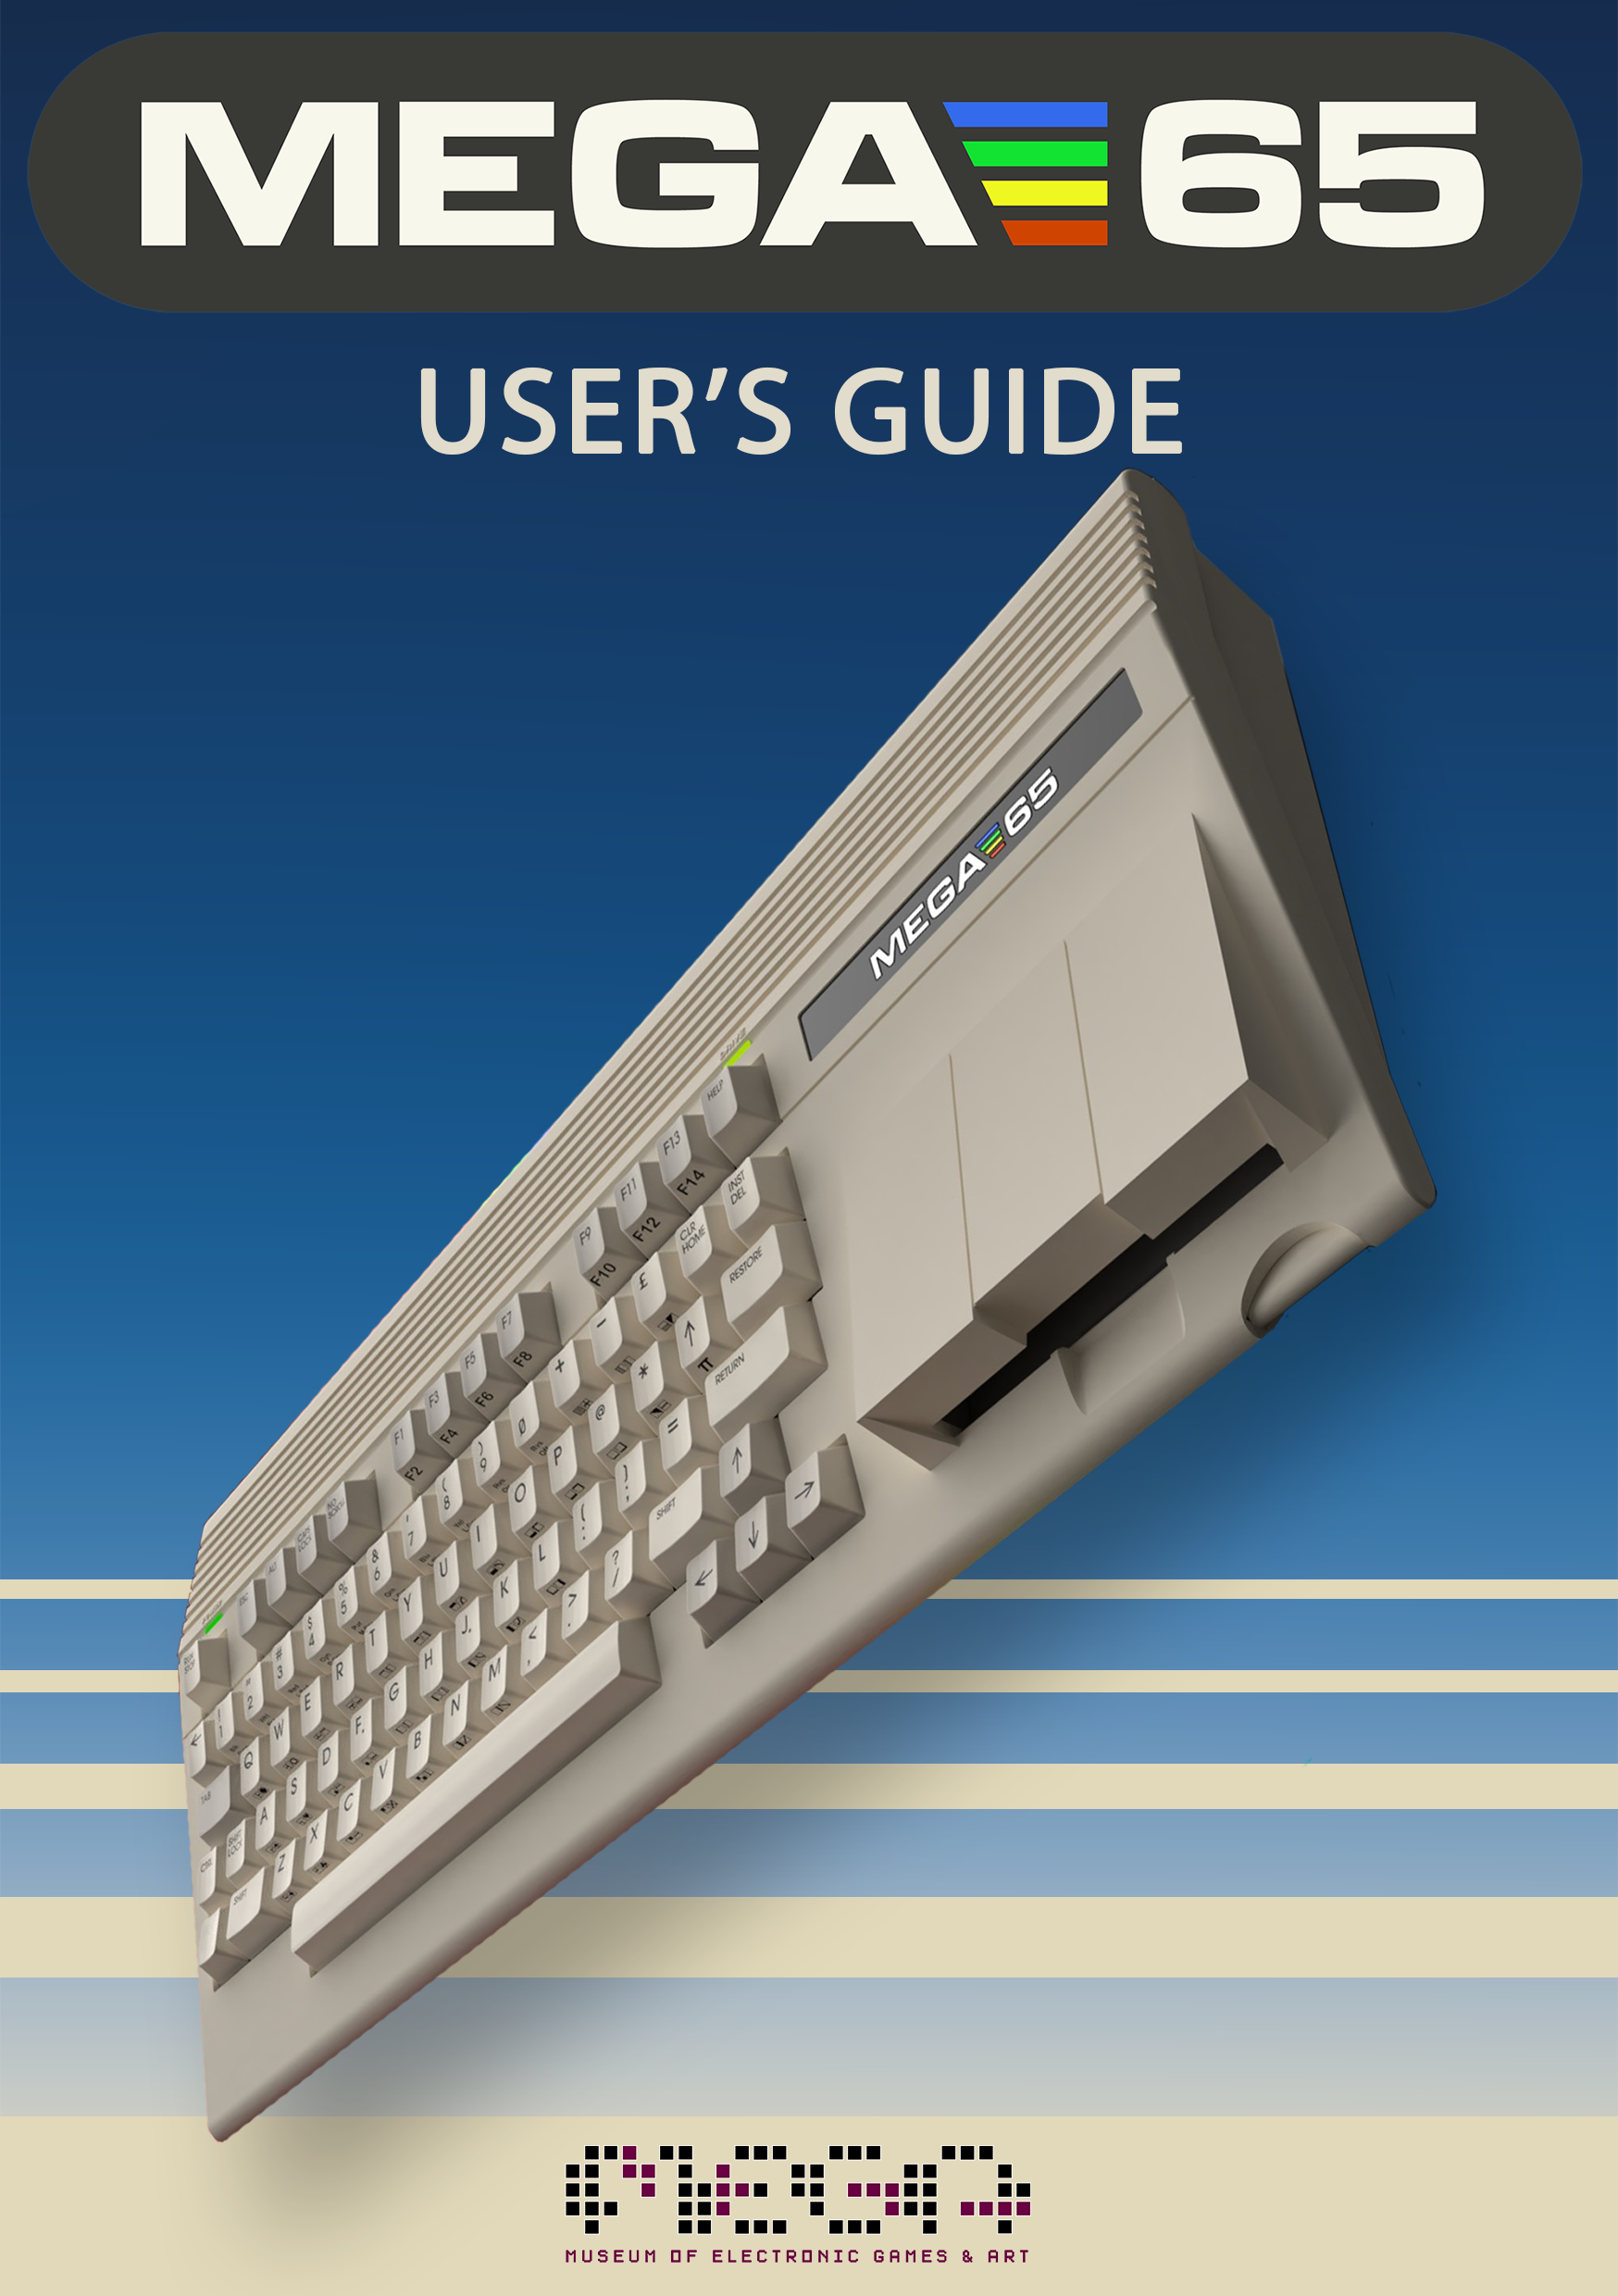
\includegraphics[height=210mm,width=149mm]{frontcover/manual_title}};
\end{tikzpicture}

%\newpage
%\pagecolor{white}

%\vspace*{-2cm}\chapter*{MEGA65 TEAM}
\newpage
{\huge MEGA65 TEAM}\vspace{1cm}

\setlength{\tabcolsep}{1mm}
\begin{tabular}{ll}

{\large\bf Dr. Paul Gardner-Stephen}    & {\large\bf Detlef Hastik} \\
\textit{(highlander)}                   & \textit{(deft)} \\
Founder                                 & Co-Founder \\
Software and Virtual Hardware Architect & General Manager \\
Spokesman and Lead Scientist            & Marketing \& Sales \\
& \\
{\large\bf Martin Streit}               & {\large\bf Anton Schneider-Michallek} \\
 \textit{(seriously)}                   & \textit{(adtbm)} \\
Video and Photo Production              & Hardware Pool Management \\
Tax and Organization                    & Soft-, Hard- and V-Hardware Testing \\
Social Media                            & Forum Administration \\
& \\
{\large\bf Falk Rehwagen}               & {\large\bf Antti Lukats} \\
 \textit{(bluewaysw)}                   & \textit{(antti-brain)} \\
Jenkins Build Automation                & Host Hardware Design and Production \\
GEOS, Hardware Quality Management       & \\
& \\
{\large\bf Dieter Penner}               & {\large\bf Dr. Edilbert Kirk} \\
 \textit{(doubleflash)}                 & \textit{(Bit Shifter)} \\
Host Hardware Review and Testing        & Manual and Tools \\
File Hosting                            & ROM Enhancements \\
& \\
{\large\bf Gábor Lénárt}                & {\large\bf Mirko H.} \\
 \textit{(LGB)}                         & \textit{(sy2002)} \\
Emulator                                & Additional Hardware and Platforms \\
& \\
{\large\bf Farai Aschwanden}            & {\large\bf Thomas Hertzler} \\
 \textit{(Tayger)}                      & \textit{(grumpyninja)} \\
File Base, Tools                        & USA Spokesman \\
Financial Advisory                      & Artist Relations \\
& \\
{\large\bf Andrew Owen}                 & {\large\bf Daniel England} \\
 \textit{(Cheveron)}                    & \textit{(Mew Pokémon)} \\
Keyboard Advisory, Sinclair Support     & Additional Code and Tools \\
& \\
{\large\bf Roman Standzikowski}         & {\large\bf Hernán Di Pietro} \\
 \textit{(FeralChild)}                  & \textit{(indiocolifa)} \\
Open ROMs                               & Additional Emulation \\
\end{tabular}


\chapter*{Reporting Errors and Omissions}

This book is a work-in-progress produced by and for the MEGA65 community.
The version of this edition is:

\input{gitinfo}

We want this book to be the best that it possibly can. So if you see any errors,
find anything that is missing, or would like more information,
please report them using the MEGA65 User's Guide issue tracker:

\url{https://github.com/mega65/mega65-user-guide/issues}

You can also check there to see if anyone else has reported a similar problem,
while you wait for this book to be updated.

Finally, you can always download the latest version of this book from:

\url{https://github.com/mega65/mega65-user-guide}




% paper title
% Titles are generally capitalised except for words such as a, an, and, as,
% at, but, by, for, in, nor, of, on, or, the, to and up, which are usually
% not capitalised unless they are the first or last word of the title.
% Linebreaks \\ can be used within to get better formatting as desired.
% Do not put math or special symbols in the title.

\cleardoublepage

\pagenumbering{roman}

\begin{titlepage}
    \pagecolor{blue}
     \begin{center}
       {
         \large
         % Put a nice amount of vertical space before the title
         \vspace*{2cm}
               {\Huge\textcolor{white}{\bf{MEGA65 REFERENCE GUIDE}}}\\
             \vspace{\fill}
                    {\textcolor{white}
                    {Published by \\ the MEGA Museum of Electronic Games \& Art e.V., Germany.}}
       }
     \end{center}
   \end{titlepage}

% Then the copyright notice page
  \pagecolor{white}\textcolor{black}
  \vfill
  WORK IN PROGRESS

  \index{copyright}Copyright \copyright 2019 -- 2021 by Paul Gardner-Stephen,
  the MEGA Museum of Electronic Games \& Art e.V.,
  and contributors.

  This reference guide is made available under the GNU Free Documentation
  License v1.3, or later, if desired. This means that you are free to
  modify, reproduce and redistribute this reference guide, subject to
  certain conditions. The full text of the GNU Free Documentation
  License v1.3 can be found at
  \url{https://www.gnu.org/licenses/fdl-1.3.en.html}.

  Implicit in this copyright license, is the permission to duplicate
  and/or redistribute this document in whole or in part for use in
  education environments. We want to support the education of future
  generations, so if you have any worries or concerns, please contact us.

   \par\today

\newpagestyle{onlynumber}{\setfoot[][{\bf\small\thepage}][]
                                  {} {\bf\small\thepage} {}}
\pagestyle{onlynumber}
\pagecolor{white}

\tableofcontents

%% XXX - big numbers are not in bold, because latex gets confused
\newcommand*{\justifyheading}{\raggedleft}
\definecolor{headingblue}{rgb}{0.5,0.5,1}

% \titleformat{command}[shape]
%   {format}
%   {label}
%   {sep}
%   {before}
%   [after]

% ***************
% PART title page
% ***************

\titleclass{\part}{top}
\titleformat{\part}[display]
   {\thispagestyle{empty}\pagecolor{blue}\normalfont\huge\bfseries\justifyheading}
   {\textcolor{white}{\fontsize{50}{65}\selectfont\bf{PART}\quad{\fontsize{100}{130}\selectfont \bf{\serifed\thepart}}}}
   {20pt}
   {\Huge\textcolor{white}}
   [\newpage\pagecolor{white}\textcolor{black}]

% ******************
% CHAPTER title page
% ******************

\titleformat{\chapter}[display]
   {\thispagestyle{empty}\pagecolor{blue}\normalfont\huge\bfseries\justifyheading}
   {\textcolor{white}{\MakeUppercase{\chaptertitlename}\quad{\fontsize{100}{130}\selectfont \bf\thechapter}}}
   {20pt}
   {\Huge\textcolor{white}}
   [{\chapmtoc\insertminitoc}\newpage\pagecolor{white}\textcolor{black}\cleardoublepage]

% ******************
% SECTION title page
% ******************

\titleformat{\section}[display]
   {\raggedright}
   {\thesection}
   {20pt}
   {\huge\bf\color{headingblue}\uppercase}
   [\color{black}]

\part{PREFACE}

\chapter{Introduction}

Congratulations on your purchase of one of the most long-awaited computers in the history of computing. The MEGA65 is a community designed computer, based on the never-released Commodore{\textregistered} 65\footnote{Commodore is a trademark of C= Holdings} computer; a computer designed in 1989 and intended for public release in 1990. Decades have passed, and the MEGA 65 invokes an earlier time when computers were simple and friendly. They were not only simple to operate and understand how they work, but friendly and approachable for new users.

These 1980s computers inspired an entire generation of professionals to choose the exciting and rewarding technology careers they have today. Just imagine the joy of these individuals as they learned they could use their new computer to solve problems, write a letter, prepare taxes, invent new things, or even discover how the universe works. We want to recreate that level of excitement not found in modern computing, so we made the {\bf MEGA65}.

The MEGA65 team believes that owning a computer is like owning a home; you don't just use a home; you change things big and small to make it your own custom living space. After a while, when you settle in, you may decide to renovate or expand your home to make it more comfortable or provide more utility. Think of the MEGA65 as a "computing home."

This guide will teach you how to do more than just hang pictures on a wall, it will ask you to build your dream home. While you read this user's guide, you will learn how to operate the MEGA65, code programs, add additional software, and extend hardware capabilities. What won't be immediately obvious is that along the journey, you will also learn about the history of computing as you explore Commodore BASIC version 10 and operating system commands.

Computer graphics and music make computing more fun; and we designed the MEGA65 for fun! In this user's guide, you will learn to code using the MEGA65's built-in {\bf graphics} and {\bf sound} capabilities. But you don't need to be a coder to have fun with the MEGA65. Because the MEGA65 includes a complete Commodore{\textregistered} 64{\texttrademark}\footnote{Commodore 64 is a trademark of C= Holdings, }, it can also run thousands of games, utilities, and business software from the past and new programs being written today by Commodore enthusiasts. Excitement for the MEGA65 will grow as we discover what programmers as they learn about the power and features of this modern Commodore computer recreation. Together, we will create a whole new "home-brew" community to do things that even we didn't think were possible when creating the MEGA65.

We welcome you on this journey! Thank you for becoming a part of the {\bf MEGA65}community of  users, coders, and enthusiasts! Get involved, learn more about your MEGA65, and join us online at:

% I thought a call to action to join the community would be good to add early on. Where will the final online community call home?


\cleardoublepage
\pagenumbering{bychapter}

\part{GETTING TO KNOW YOUR MEGA65}

\chapter{SETUP}
\phantomsection
\section{Unpacking and connecting the MEGA65}

Time to set up your MEGA65 home computer.
The box contains the following:
\begin{itemize}
\setlength\itemsep{-0.75mm}
\item MEGA65 computer.
\item Power supply (black box with socket for mains supply).
\item This book, the MEGA65 User's Guide.
\end{itemize}

In addition, to be able to use your MEGA65 computer you may need:
\begin{itemize}
	\item A television or computer monitor with a VGA or digital video input, that is capable of displaying an image with 480p or 576p (720x480 or 720x576 pixel resolution at 50Hz or 60Hz).
\item A VGA video cable, or;
\item A digital video cable.
\end{itemize}

These items are not included with the MEGA65.

You may also like to use the following to get the most out of your MEGA65:
\begin{itemize}
\item 3.5mm mini-jack audio cable and suitable speakers or hifi system, so that you can enjoy the sound capabilities of your MEGA65.
\item RJ45 Ethernet cable (regular network cable) and a network router or switch. This allows the usage of the high-speed networking capabilities of your MEGA65.
\end{itemize}

\section{Rear Connections}

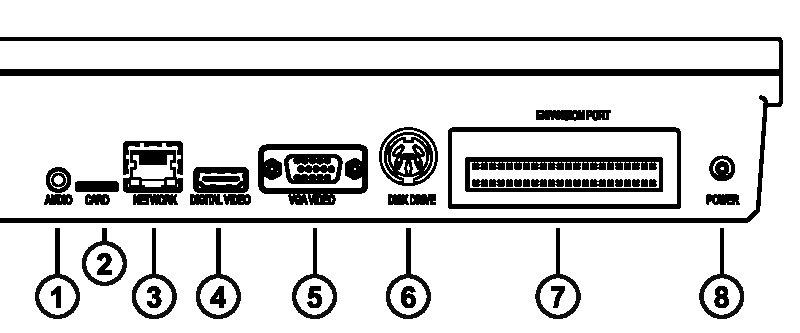
\includegraphics[width=\linewidth]{images/illustrations/mega65-rear.pdf}

\begin{center}
\setlength{\def\arraystretch{1.5}\tabcolsep}{6pt}
\begin{longtable}{ c | l}

	1	& 	3.5mm Audio Mini-Jack \\
	2	& 	SD Card Slot\\
	3	& 	Network LAN Port \\
	4	& 	Digital Video Connector \\
	5	& 	VGA Video Connector \\
	6	& 	External Floppy Disk Drive Connector \\
	7	& 	Cartridge Expansion Port \\
	8	& 	DC Power-In Socket \\

\end{longtable}
\end{center}

\newpage

\section{Side Connections}

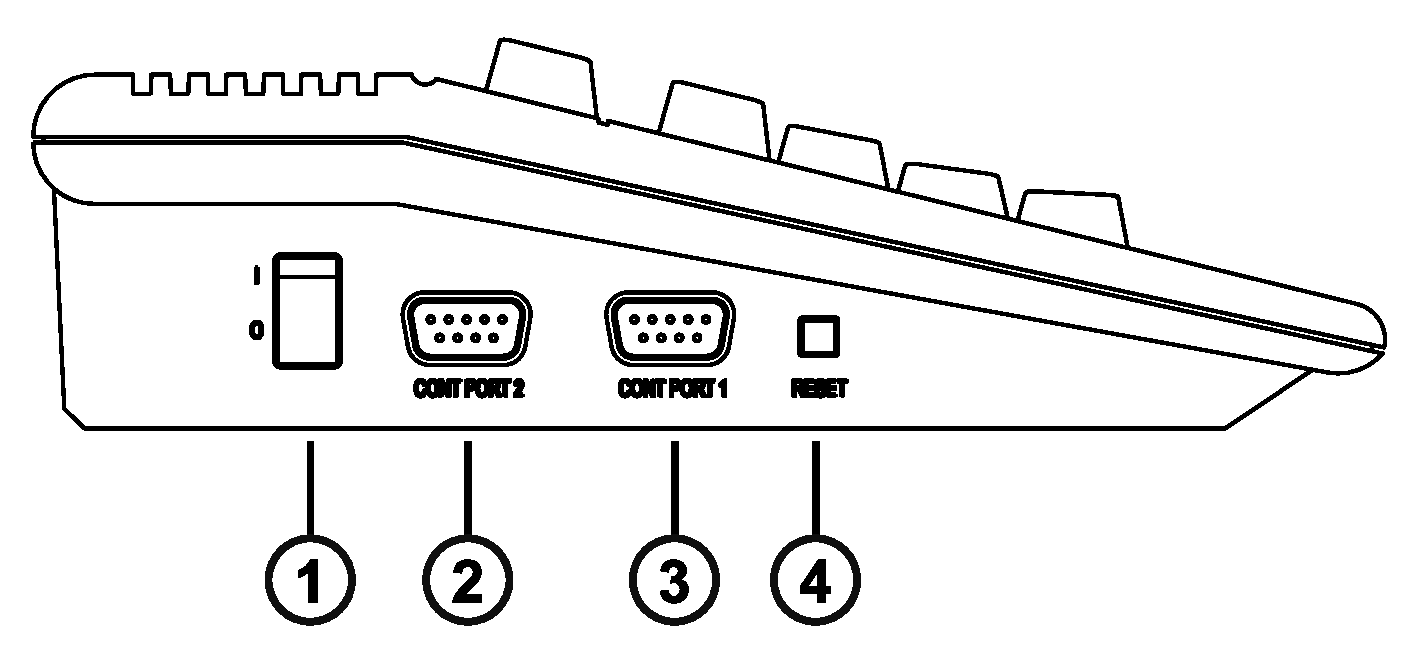
\includegraphics[width=\linewidth]{images/illustrations/mega65-side.pdf}

\begin{center}
\setlength{\def\arraystretch{1.5}\tabcolsep}{6pt}
\begin{longtable}{ c | l}

	1	& 	Power Switch \\
	2	& 	Controller Port 2 \\
	3	& 	Controller Port 1 \\
	4	& 	Reset Button \\

\end{longtable}
\end{center}

Various peripherals can be connected to Controller Ports 1 and 2 such as joysticks or paddles.

\newpage

\section{Installation}

\subsection{Connecting your MEGA65 to a screen and peripherals}

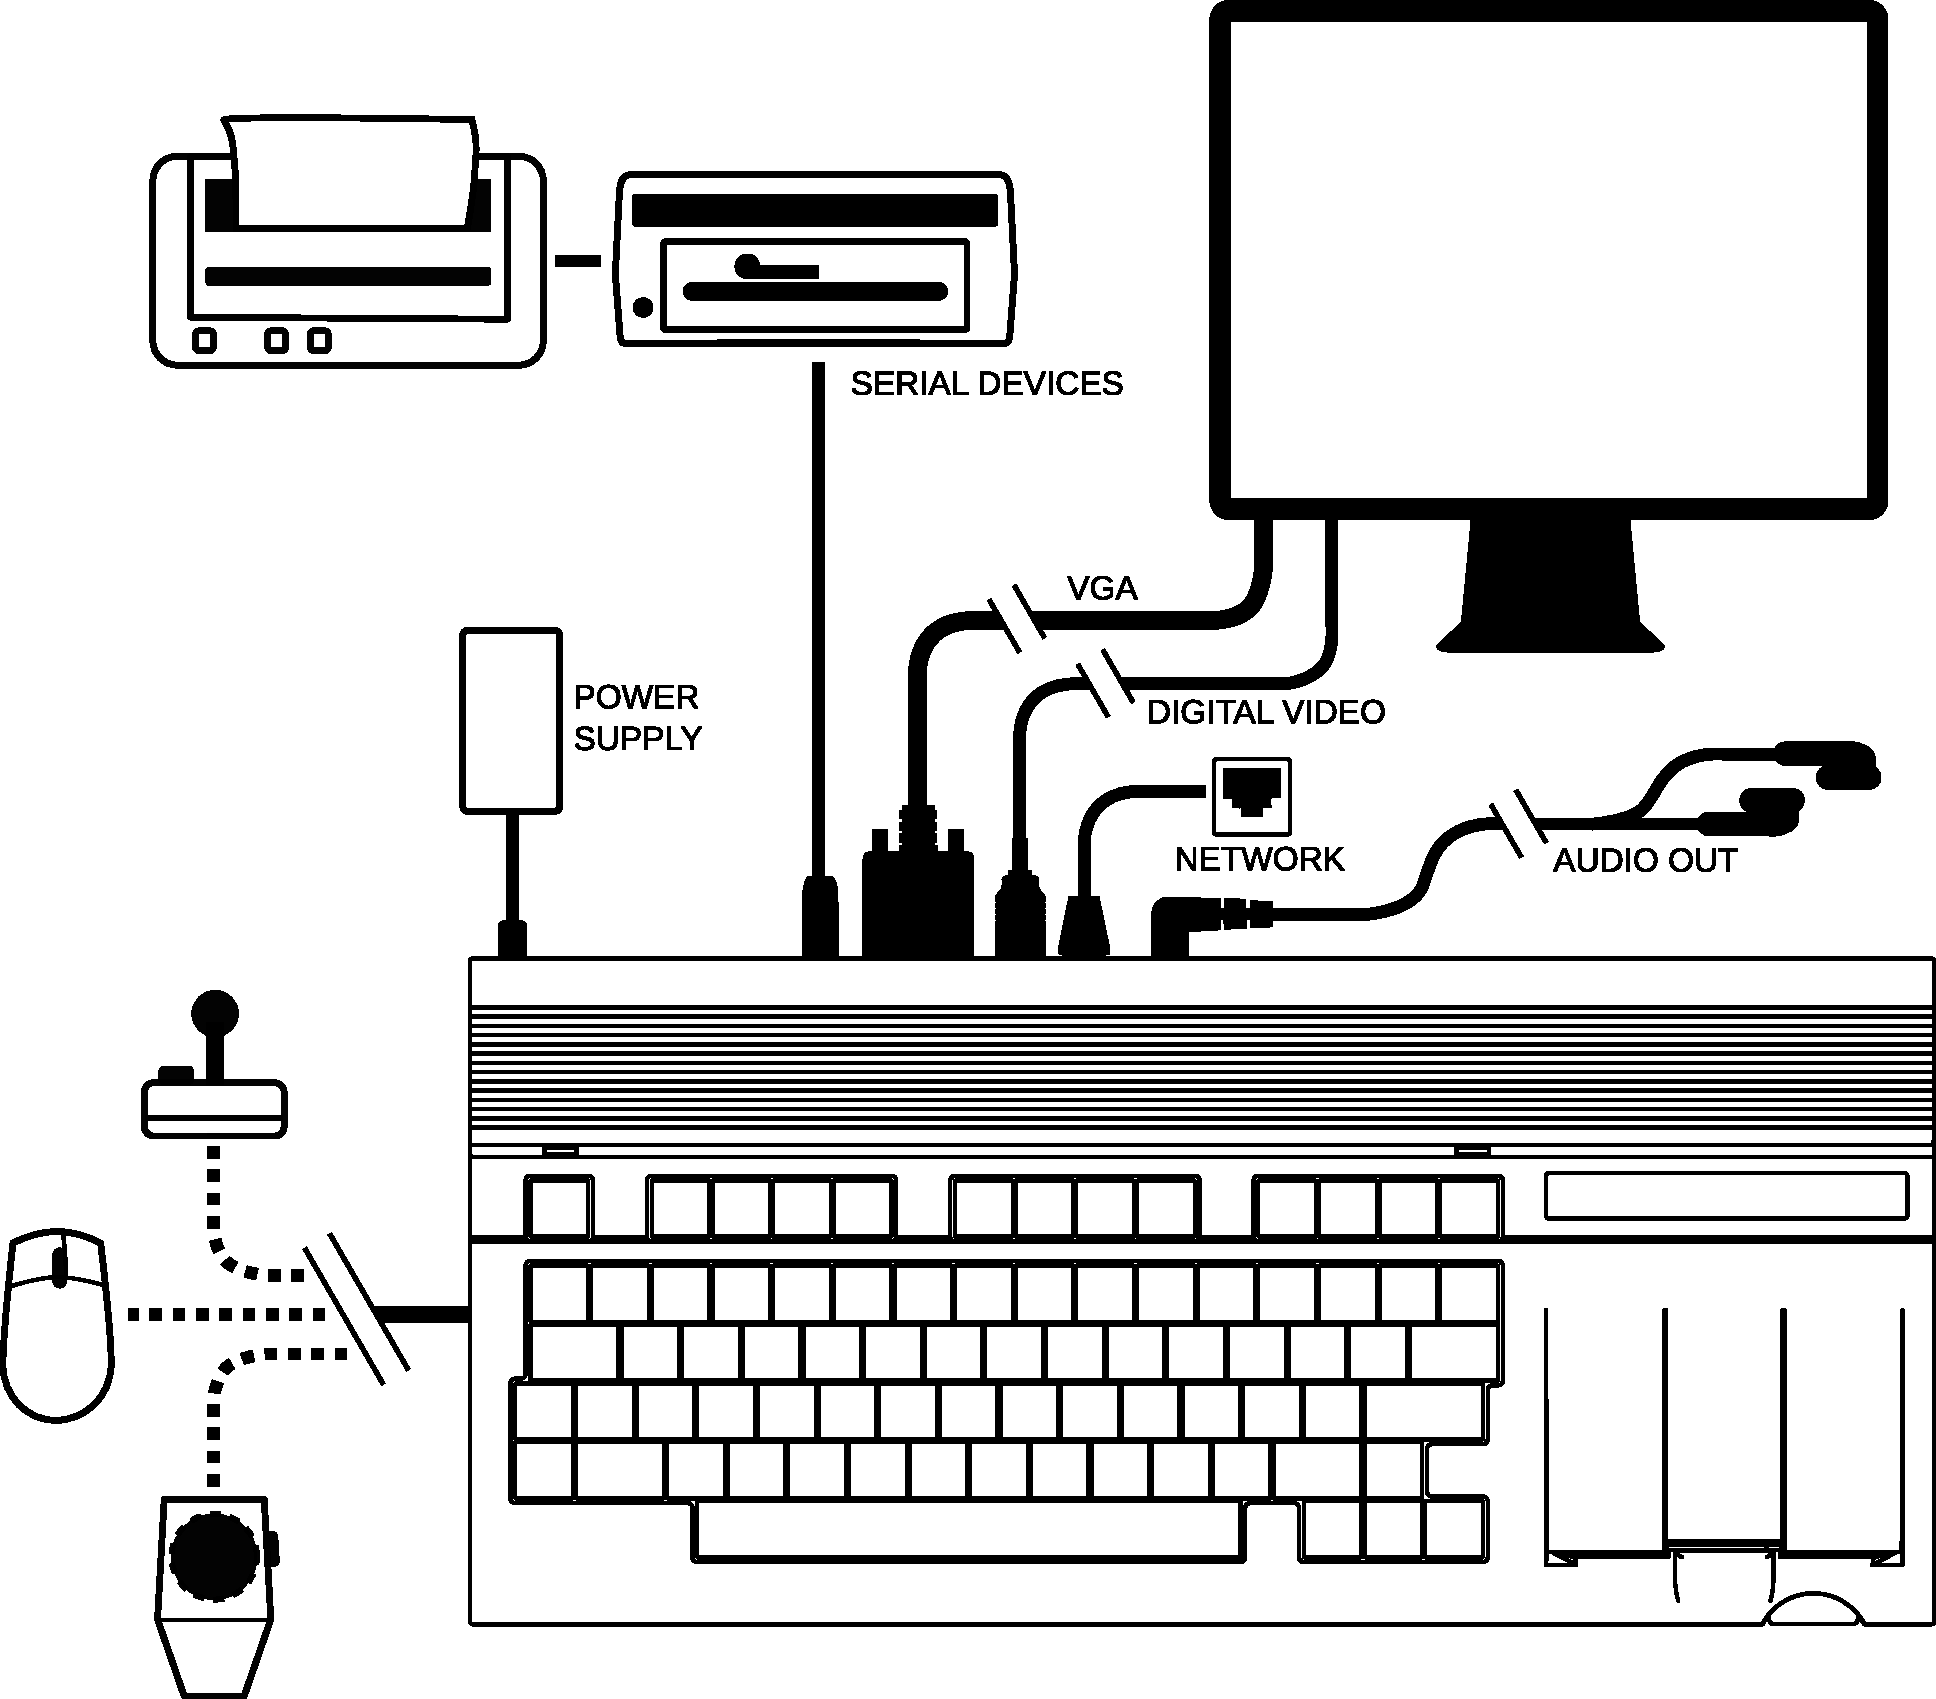
\includegraphics[width=\linewidth]{images/illustrations/mega65-top.pdf}

\newpage

\begin{enumerate}
	\item Connect the power supply to the Power Supply socket of the MEGA65.
	\item If you have a VGA monitor and a VGA cable, connect one end to the VGA port of the MEGA65 and the other end into your VGA monitor.
	\item If you have a TV or monitor with a compatible Digital Video connector, connect one end of your cable to the Digital Video port of the MEGA65, and the other into the Digital Video port of your monitor. If you own a monitor with a DVI socket, you can use a DVI to Digital Video adaptor.
\end{enumerate}

\section{Optional Connections}

\begin{enumerate}
	\item The MEGA65 includes an internal 3.5" floppy disk drive. You can also connect older Commodore{\textregistered} IEC serial floppy drives to the MEGA65, such as the Commodore{\textregistered} 1541, 1571 or 1581. To use these drives, connect one end of your IEC cable to the Commodore{\textregistered} floppy disk drive and the other end to the Disk Drive socket of the MEGA65. You can also connect SD2IEC devices and Pi1541's. It is possible to daisy-chain additional floppy disk drives or Commodore{\textregistered} compatible printers.
	\item You can connect your MEGA65 to an Ethernet network using a standard Ethernet cable.
	\item For enjoying audio from your MEGA65, you can connect a 3.5mm stereo mini-jack cable to an audio amplifier or speaker system. If your system has RCA connectors you will need a 3.5mm mini-jack to twin RCA adaptor cable. The MEGA65 also has a built in amplifier to allow the use of headphones.
	\item A Secure Digital Card or SD Card (SDHC and SDXC) can be inserted into the SD Card slot at the rear of the MEGA65 as a drive.
\end{enumerate}


\section{Operation}

\subsection{Using the MEGA65}

\begin{enumerate}
	\item Turn on the MEGA65 by using the switch on the left hand side.
	\item After a moment, the following will be displayed on your TV or monitor:
\end{enumerate}

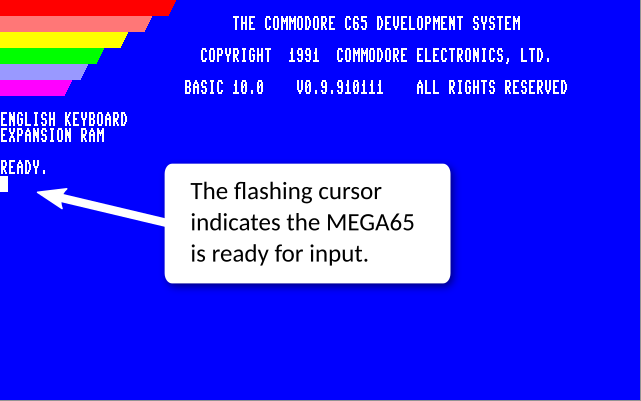
\includegraphics[width=\linewidth]{images/introduction-screen/switched-on.png}

\subsection{THE CURSOR}

The flashing square underneath the READY prompt is called the cursor. The cursor indicates that the computer is ready to accept input. Pressing keys on the keyboard will print that character onto the screen. The character will be printed at the current cursor position, and the cursor will advance to the next position.

You can type commands, for example: telling the computer to load a program. You can even start entering program code.

\chapter{Getting Started}
\phantomsection
\section{Keyboard}
\label{cha:getting-started}

Now that everything is connected, it's time to get familiar with the MEGA65 keyboard.

You may notice that the keyboard is a little different from the keyboards used on computers today. While most keys will be in familiar positions, there are some specialised keys, and some with special graphic symbols marked on the front.

Here's a brief description of how some of these special keys function.

\subsection{Command Keys}

The Command Keys are: \specialkey{RETURN}, \specialkey{SHIFT}, \specialkey{Ctrl}, \megasymbolkey and \widekey{RESTORE}.

\subsubsection{RETURN}

Pressing the \specialkey{RETURN} key enters the information you have typed into the MEGA65's memory. The computer will either act on a command, store some information, or display an error message if you made a mistake.

\subsubsection{SHIFT}

The two \specialkey{SHIFT} keys are located on the left and the right. They work very much like the Shift key on a regular keyboard, however they also perform some special functions as well.

In upper case mode, holding down \specialkey{SHIFT} and pressing any key with a graphic symbol on the front produces the right-hand symbol on that key. For example, \specialkey{SHIFT} and \megakey{J} prints the \graphicsymbol{J} character.

In lower case mode, pressing \specialkey{SHIFT} and a letter key prints the upper case letter on that key.

Finally, holding down the \specialkey{SHIFT} key and pressing a Function key accesses the function shown on the front of that key. For example: \specialkey{SHIFT} and \megakey{F1} activates \textbf{F2}.


\subsubsection{SHIFT LOCK}

In addition to the Shift key is \specialkey{SHIFT\\LOCK}. Press this key to lock down the Shift function. Now any key you press while the Shift Lock key is illuminated prints the character to the screen as if you were holding down \specialkey{SHIFT}. This includes special graphic characters.

\subsubsection{CTRL}

\specialkey{CTRL} is the Control key. Holding down \specialkey{CTRL} and pressing another key allows you to perform Control Functions. For example, holding down \specialkey{CTRL} and one of the number keys allows you to change text colours. The colour that is printed at the top row on the front of the number key will be used.

There are some examples of this in \bookvref{sec:screen-editor}, and all the Control Functions are listed in \bookvref{appendix:controlcodes}.

If a program is being LISTed to the screen, holding down \specialkey{CTRL} slows down the display of each line.

Holding \specialkey{CTRL} and pressing \megakey{*} enters the Matrix Mode Debugger.

\subsubsection{RUN/STOP}

Normally, pressing the \specialkey{RUN\\STOP} key stops execution of a program. Holding \specialkey{SHIFT} while pressing \specialkey{RUN\\STOP} loads the first program from disk.

Programs are able to disable the \specialkey{RUN STOP} key.

You can boot your MEGA65 into the machine code monitor by holding down \specialkey{RUN\\STOP} and pressing reset on the left-hand side.

\subsubsection{RESTORE}

The computer screen can be restored to a clean state without clearing the memory by holding down the \specialkey{RUN\\STOP} key and pressing \widekey{RESTORE}. This combination also resets operating system vectors and re-initialises the screen editor, which makes it a handy combination if the computer has become a little confused.

Programs are able to disable this key combination.

You can also enter the Freeze Menu by holding down \widekey{RESTORE} for more than one second. You can then access the machine code monitor via the Freeze menu.

\newpage

\subsubsection{THE CURSOR KEYS}

At the bottom right-hand side of the keyboard are the cursor keys. These four directional keys allow you move the cursor to any position for on-screen editing.

The cursor moves in the direction indicated on the keys: \megakey{$\leftarrow$} \megakey{$\uparrow$} \megakey{$\rightarrow$} \megakey{$\downarrow$}

However, it is also possible to move the cursor up using \specialkey{SHIFT} and \megakey{$\downarrow$}. In the same way you can move the cursor left using \specialkey{SHIFT} and \megakey{$\rightarrow$}.

You don't have to keep pressing a cursor key over and over. If you need to move the cursor a long way, you can keep the key pressed down. When you are finished, simply release the key.

\subsubsection{INSerT/DELete}

This is the INSERT / DELETE key. When pressing \specialkey{INST\\DEL}, the character to the left is deleted, and all characters to the right are shifted one position to the left.

To insert a character, hold the \specialkey{SHIFT} key and press \specialkey{INST\\DEL}. All the characters to the right of the cursor are shifted to the right. This allows you to type a letter, number or any other character into the newly inserted space.


\subsubsection{CLeaR/HOME}

Pressing the \specialkey{CLR\\HOME} key returns the cursor into the top left-most position of the screen.

Holding down \specialkey{SHIFT} and pressing \specialkey{CLR\\HOME} clears the entire screen and places the cursor into the top left-most position of the screen.

\subsubsection{MEGA KEY}

The \megasymbolkey key or the MEGA key provides a number of different functions and can be used to launch special utilities.

Holding the \specialkey{SHIFT} key and pressing \megasymbolkey switches between lower and upper-case character modes.

Holding \megasymbolkey and pressing any key with graphic symbols on the front prints the left-most graphic symbol to the screen.

Holding \megasymbolkey and pressing any key that shows a single graphic symbol on the front prints that graphic symbol to the screen.

Holding \megasymbolkey and pressing a number key switches to one of the colours in the second range. The colour that is printed at the bottom row on the front of the number key will be used.

Holding \megasymbolkey and pressing \specialkey{TAB} enters the Matrix Mode Debugger.

Switching on the MEGA65 or pressing the reset button on the left-hand side while holding down \megasymbolkey switches the MEGA65 into C64 mode.

\subsubsection{NO SCROLL}
If a program is being LISTed to the screen, pressing \specialkey{NO\\SCROLL} freezes the screen output. This feature is not available in C64 mode.


\subsection{Function Keys}

There are seven Function keys available for use by software applications, \megakey{F1} \megakey{F3} \megakey{F5} \megakey{F7} \megakey{F9} \megakey{F11} and \megakey{F13} can be used to perform functions with a single press.

Hold \specialkey{SHIFT} to access \megakey{F2} through to \megakey{F14} as shown on the front of each Function key.

Only Function keys \megakey{F1} to \megakey{F8} are available in C64 mode.

\subsubsection{HELP}

The \specialkey{HELP} key can be used by software and acts as an \megakey{F15} / \megakey{F16} key.

\subsubsection{ALT}

Holding \specialkey{ALT} down while pressing other keys can be used by software to perform functions. Not available in C64 mode.

Holding \specialkey{ALT} down while switching the MEGA65 on activates the Utility Menu. You can format an SD card, or enter the MEGA65 Configuration Utility to select the default video mode and other settings, or test your keyboard.

\subsubsection{CAPS LOCK}

The \specialkey{CAPS\\LOCK} works like \specialkey{SHIFT\\LOCK} in C65 and MEGA65 modes, but only modifies the alphabet keys.
Also, holding the \specialkey{CAPS\\LOCK} key down forces the processor to run at the maximum speed. This can be used, for example,
to speed up loading from the internal disk drive or SD card, or to greatly speed up the de-packing process after a program is run.
This can reduce the loading and de-packing time from many seconds to as little as a fraction of a second.

\section{The Screen Editor}
\label{sec:screen-editor}

When you switch on your MEGA65 or reset it, the following screen will appear:

\begin{center}
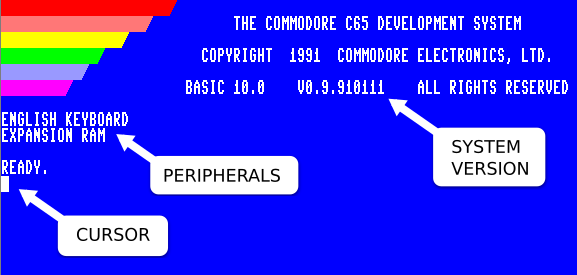
\includegraphics[width={10cm}]{images/introduction-screen/layout.png}
\end{center}

The colour bars in the top left-hand side of the screen can be used
as a guide to help calibrate the colours of your display.
The screen also displays the name of the system,
the copyright notice, and the ROM version.
The displayed date and time are taken from the internal RTC
(Real-Time Clock), which can be set in the Configure Menu.

Finally, you will see the \screentext{READY} prompt and the flashing cursor.

You can begin typing keys on the keyboard and the characters will be
printed at the cursor position. The cursor itself will advance after
each key press.

You can also produce reverse text or colour bars by holding down \specialkey{CTRL} and pressing \megakey{9}, or \megakey{R}. This enters reverse text mode. When this is enabled, you can press and hold the \megakey{Space} bar. While doing so, a white bar will be drawn across the screen.
\index{Keyboard!CTRL}
You can even change the current colour by holding \specialkey{CTRL} down and pressing a number key (from \megakey{1} to \megakey{8}). For example, if you press and hold \specialkey{CTRL} down and press \megakey{1}, the colour will change to black. Now, when you hold down the \megakey{Space} bar, a black bar will be drawn. If you continue to change the colour and press the \megakey{Space} bar, you will get an effect similar to the image below:


\begin{center}
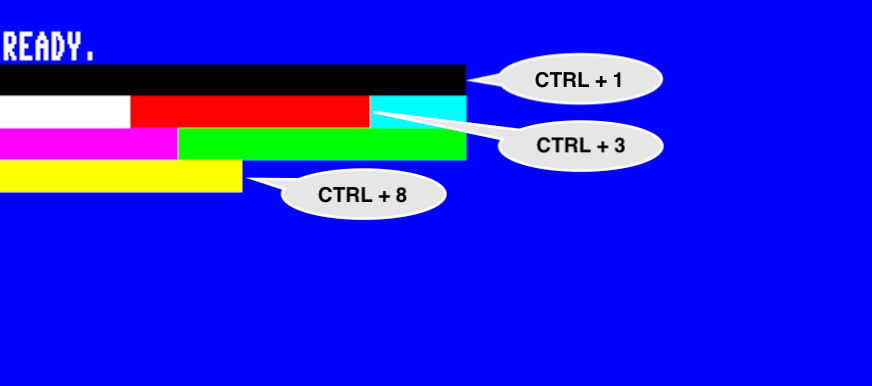
\includegraphics[width={10cm}]{images/introduction-screen/colour-bars.png}
\end{center}


\index{Keyboard!MEGA Key}
You can disable reverse text mode by holding \specialkey{CTRL} and pressing \megakey{0}.

By pressing any key, characters will be printed to the screen in the chosen colour.

A further eight colours can be selected by holding down \megasymbolkey and pressing a key from \megakey{1} to \megakey{8}.
The colour that is printed at the bottom row on the front of the number key will be used. For example, if you held
\megasymbolkey down while pressing \megakey{4}, dark gray will be used. For even more colours, see \bookvref{appendix:escape-colours}.

\needspace{4cm}
You can create fun pictures just by using these colours and letters.  Here's an example of what a year four student drew:

\begin{center}
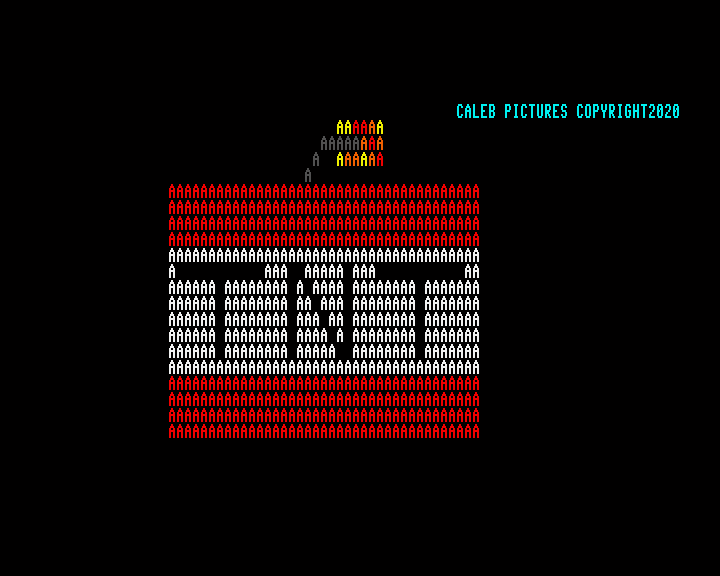
\includegraphics[width={6cm}]{images/caleb-PETSCII-TNT-final}
\end{center}

What will you draw?

\needspace{2cm}
\textbf{Functions}

Functions using \specialkey{CTRL} are called \textbf{Control Codes}.
Functions using \megasymbolkey are called \textbf{Mega Codes}. There are also functions that are called by using \specialkey{SHIFT}, which
are called \textbf{Shifted Codes}.

Lastly, \specialkey{ESC} enables the use of \textbf{Escape Sequences}.

You can read about all of these functions in detail in \bookvref{appendix:controlcodes}, but some are shown in this section.


\needspace{2cm}
\textbf{ESC Sequences}
\index{Keyboard!Escape Sequences}
Escape sequences are performed a little differently than a Control function or a Shift function. Instead of holding the modifier key down, an Escape sequence is performed by pressing \specialkey{ESC} and releasing it, followed by pressing the desired key code.

For example: to switch between 40/80 column mode, press and release \specialkey{ESC}, then press \megakey{X}.

There are more modes available. You can create flashing text by holding \specialkey{CTRL} down and pressing \megakey{O}. Any characters you type in will flash. Turn flash mode off by pressing \specialkey{ESC},  then \megakey{O}.



\section{Editor Functionality}


The MEGA65 screen can allow you to do advanced tabbing, and quickly move around the screen in many ways to help you to be more productive.

For example, press \specialkey{CLR HOME} to go to the home position on the screen. Hold \specialkey{CTRL} down and press \megakey{W} several times. This is the \textbf{Word Advance function}, which jumps your cursor to the next word, or printable character.

You can set custom tab positions on the screen for your convenience. Press \specialkey{CLR HOME} and then \megakey{$\rightarrow$} to the fourth column. Hold down \specialkey{CTRL} and press \megakey{X} to set a tab. Move another 16 positions to the right again, and press \specialkey{CTRL} and \megakey{X} again to set a second tab.

Press \specialkey{CLR HOME} to go back to the home position. Hold \specialkey{CTRL} down and press \megakey{I}. This is the \textbf{Forward Tab function}. Your cursor will tab to the fourth position. Press \specialkey{CTRL} and \megakey{I} again. Your cursor will move to position 8. Why do you ask? By default, every 8th position is already set as a tabbed position. So the 4th and 20th positions have been added to the existing tab positions. You can continue to press \specialkey{CTRL} and \megakey{I} to advance to the 16th and 20th positions.

To find the complete set of Control codes, see \bookvref{appendix:controlcodes}.

\textbf{Creating a Window}
\index{Keyboard!Escape Sequences}

You can set a window on the MEGA65 working screen. Move your cursor to the beginning of the "BASIC 65" text. Press \specialkey{ESC}, then press \megakey{T}. Move the cursor 10 lines down and 15 to the right.

Press \specialkey{ESC}, then \megakey{B}. Anything you type will be contained within this window.

For example, if you were to type \screentext{LIST} to list out a program, the listing will be confined to the window region you have specified:

\begin{center}
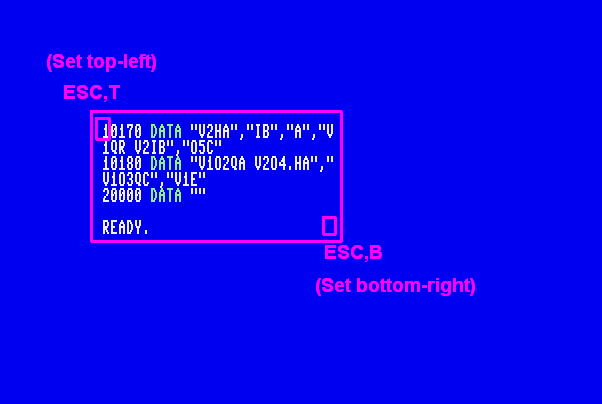
\includegraphics[width={7cm}]{images/set-window.png}
\end{center}

To escape from the window back to the full screen, press \specialkey{CLR HOME} twice.


\textbf{Extras}

Below are some extra, useful things you can do whilst in the screen editor:

  To enter the \textbf{Freeze Menu}, long press on \widekey{RESTORE}, then press \megakey{J} to switch joystick ports without 
having to physically swap the joystick to the other port. You can read more about the Freeze Menu, and what else it can do
on page \pageref{sec:freezer}.

\index{POKE}
  To enter \textbf{Fast mode} (40.5MHz), either type \screentext{SPEED} (preferred way), or \screentext{POKE 0,65} or enter the Freeze Menu and switch the CPU frequency with \megakey{F}.

  Return back to \textbf{Slow mode} (1MHz) by either typing \screentext{SPEED 1} (preferred way), or \screentext{POKE 0,64} or enter the Freeze Menu and switch the CPU frequency with \megakey{F}.

  \megasymbolkey + \specialkey{SHIFT} switches between uppercase and lowercase text for the entire display.

\chapter{Configuring your MEGA65}
\label{cha:configuring}

\section{Preparing for First Use: Formatting SD Cards}

The MEGA65 has two SD card slots: A full-size SD card slot inside, next to
the trap-door, and a microSD size slot on the rear.  The current version
of the MEGA65 firmware only supports the use of one SD card at a time.
If you have cards in both slots, the MEGA65 will use the external microSD
slot in preference.  The exception to this, is that the MEGA65's FDISK/FORMAT
utility can access both, allowing you to select which you wish to format or
repair.

Depending on the model, your MEGA65 may or may not come with a pre-configured SD card.
If it doesn't, or if you wish to use a different SD card, e.g., with a
larger capacity, you must first format it for use in the MEGA65.

{\em This must be done in the MEGA65, not in a PC or other computer.}

{\em Only SDHC cards should be used. Older SD cards (typically with
  a capacity of <4GB) will not work.  Newer SDXC cards with
  capacities greater than 32GB may or may not work.  We would
  appreciate hearing your experience with such cards. It is unimportant
  what file-system is currently on the card, as the MEGA65
  FDISK/FORMAT utility will completely reformat the card.}

There are several reasons for this: First, in order to fit the most
features into the MEGA65's small operating system, it is
particular about the FAT32 file system it uses. Second, only the
MEGA65 FDISK/FORMAT utility can create a MEGA65 System Partition. The
MEGA65 System Partition holds non-volatile configuration settings for
your MEGA65, and also contains the freeze slots, that make it easy to
switch which programme or game you are running on your MEGA65.

Fortunately, formatting an SD card on the MEGA65 is very easy.

First, power the MEGA65 on while holding down the \megakey{ALT} key.
This will present the MEGA65 Utility Menu, which contains a
selection of built-in utilities, similar to the following:

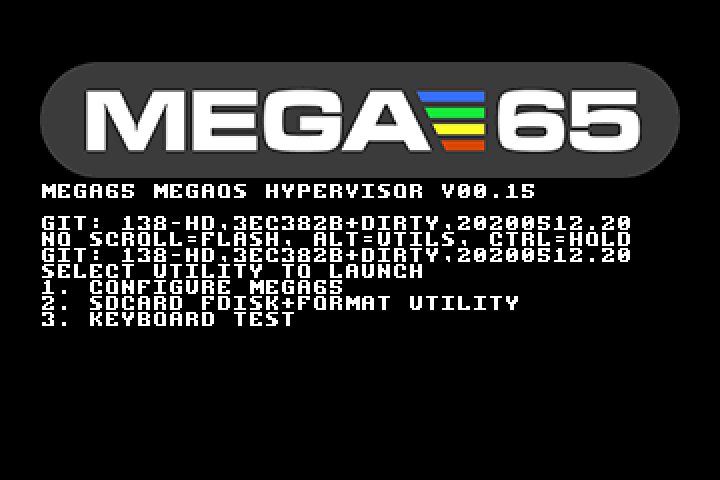
\includegraphics[width=\linewidth]{images/ss-utilmenu.png}

{\em Note that Utility Menu is always accessible, even if no SD card is present in both internal and external slots.}

The exact set of utilities
depends on the model of your MEGA65 and the version of the MEGA65
factory core which it is running. However, all versions include both
the MEGA65 FDISK/FORMAT utility, and the MEGA65 Configure utility.
Most models also include a keyboard test utility, that you can use
to test that your keyboard is functioning correctly.  This is
the same utility used in the factory when testing brand
new keyboards.

Select the number that corresponds to the FDISK/FORMAT utility.  This
will typically be 2.  The FDISK utility will start, and attempt to
detect the size of all SD cards you have installed.  If you have both
an internal and external SD card installed, it will allow you to
choose which one you wish to format. The internal SD card is bus 1,
and the external card is bus 0.  Note that the MEGA65 will
always attempt to boot using an external microSD card, if one is
installed.

For safety when formatting we {\em strongly} recommend
that you remove any SD card or microSD card that you do not intend to
format, so that you do not accidentally destroy any data.  This is
because formatting an SD card in the MEGA65 cannot be undone, and you
all data currently on the SD card {\em will be lost}.  If you
have files or data on the SD card that you wish to retain, you
should first back this up.  The contents of the FAT32
partition can be easily backed up by inserting the SD card into
another computer.  The contents of the MEGA65 System Partition,
including the contents of freeze slots requires the use of specialised
software.

You should aim to backup valuable data from your
MEGA65 on a regular basis, especially while the computer remains under
development.  While we take every care to avoid data corruption or
other mishaps, we cannot guarantee that the MEGA65 is free of bugs in
this regard.

If you have only an internal SD card, you might see a
display similar to the following:

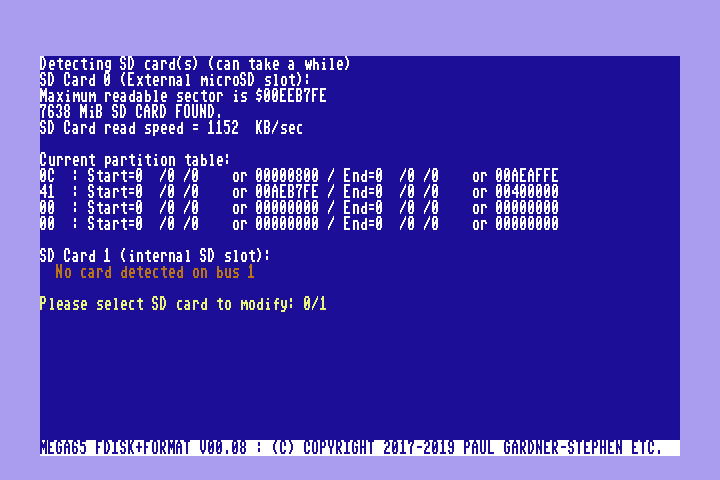
\includegraphics[width=\linewidth]{images/ss-m65fdisk-busselect.png}

Once you have selected the bus, the FDISK/FORMAT utility asks you
to confirm that you wish to delete everything:

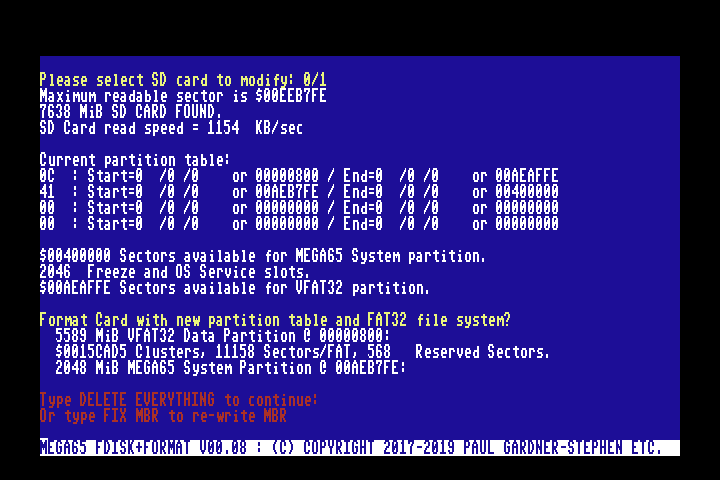
\includegraphics[width=\linewidth]{images/ss-m65fdisk-typesomething.png}

To avoid accidentally loss of data, you
must type ``DELETE EVERYTHING'' in capitals and press
\megakey{RETURN}.  Alternatively, turn the MEGA65 off and on to
abort this process without causing damage to your data.

It is also possible to attempt to recover from a lost Master Boot
Record (``Boot Sector'') by instead typing ``FIX MBR,'' should the
need arise.


As an end result, we want to have a correctly formatted SD card with the essential files stored on it for MEGA65 to boot from.

This is how it works: When powering on, MEGA65 will search for- and boot these files:
o FREEZER.M65
o AUDIOMIX.M65
o C64THUMB.M65
o C65THUMB.M65
o MEGA65.ROM
o MEGA65.D81 (default disk image, automatically mounted during start)

Straight out-of-the-box, MEGA65 will only have one SD card installed, located inside behind the trap-door. This SD card contains the essential files to properly boot from.
When an external microSD card is inserted, MEGA65 consider the external one as higher priority and will try to boot from it.
That means that the microSD card needs to have the essential files on it, otherwise MEGA65 cannot boot properly and will fall back into loading the OpenROM which does not support all the MEGA65 features.
In general, if MEGA65 cannot boot properly and fall back to OpenROM, it will be shown in the power-up screen, similar to this:

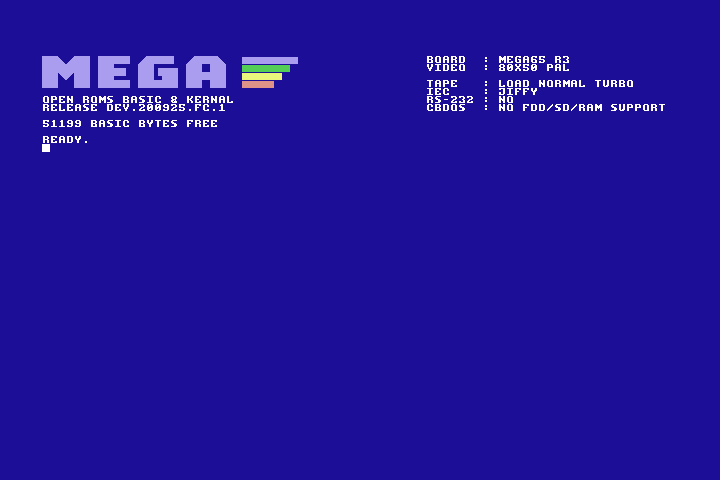
\includegraphics[width=\linewidth]{images/mega65_OpenROM_boot_noSD.png}


\section{Installing ROM and Other Support Files}

The MEGA65 FDISK/FORMAT utility will install a version of the
open-source OpenROM project's C64-compatible ROMs as part of the
formatting process. However, you may have other ROMs that you wish to
use on the MEGA65. The 911001 version of the C65 ROM in
particular is known to work well with the MEGA65.
You can copy as many of these as you wish onto the
SD card.  Make sure that they have the .ROM extension.  The default ROM
should be called MEGA65.ROM.  These files
should be 128KB in size, and use the same internal format as ROMs
intended for the C65.  This means that the C64-mode KERNAL should be
placed at offset \$E000, a C65-mode BASIC at \$A000, and a suitable
character set at \$D000.  

Other important files include FREEZER.M65 and AUDIOMIX.M65, which
allow you to use the MEGA65's integrated freezer.  You can download
the full set of support files for the MEGA65 from:

\url{https://github.com/mega65/mega65-files}

\section{Configuring your MEGA65}

The configuration utility for the MEGA65 fills a similar purpose to the BIOS on a
PC, and allows you to control certain default behaviours of your
MEGA65. However, rather than storing the configuration data in a
battery-backed RAM, it stores them on sector 1 of the SD card. This means
that if you switch SD cards, you will change the configuration data that you are using.

To enter the configuration utility, turn the MEGA65 on while
holding the \megakey{ALT} key.  This will show the utility menu,
similar to the following:

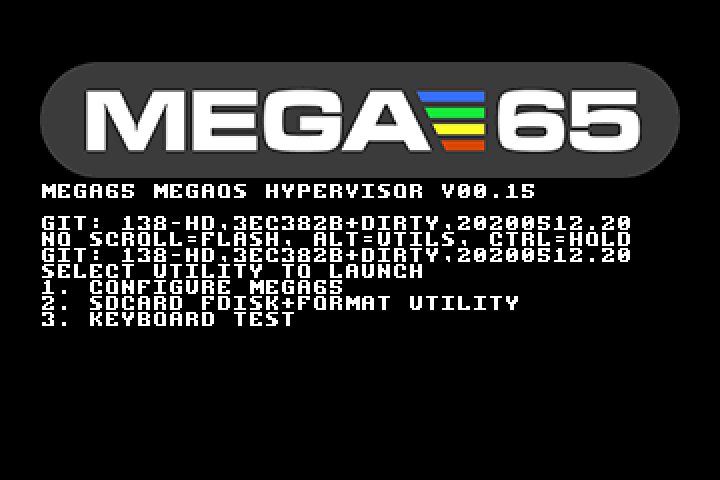
\includegraphics[width=\linewidth]{images/ss-utilmenu.png}

Now press the number corresponding to the Utility Menu.  The MEGA65
Configuration Utility will launch, showing a display similar to
the following:

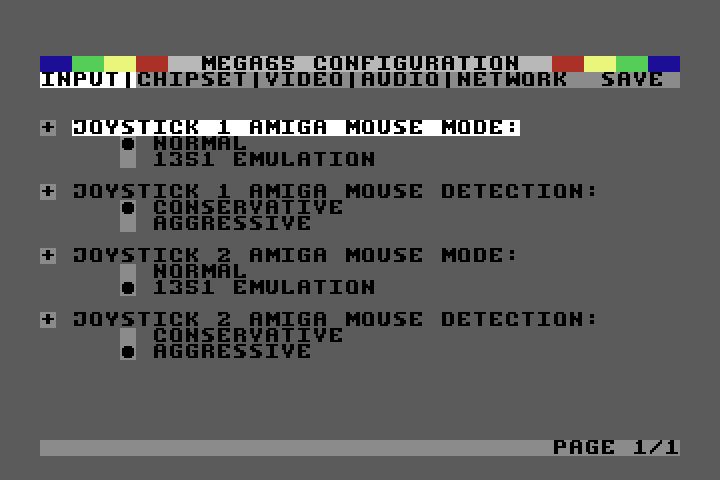
\includegraphics[width=\linewidth]{images/ss-m65config-1.png}

If your MEGA65's System Partition has become corrupt, you may be
prompted to press \megakey{F14} to correct this, i.e., hold \megakey{SHIFT} and tap
the \megakey{F13} key, with a display like the following:

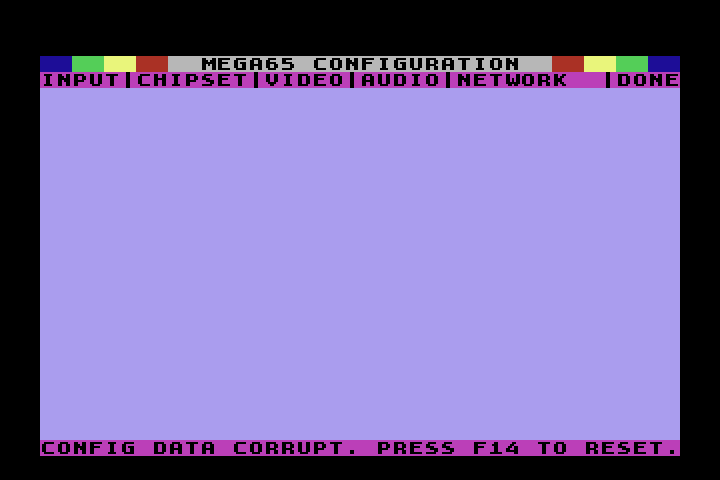
\includegraphics[width=\linewidth]{images/ss-m65config-corrupt.png}

If you do, you will
need to use \megakey{F7} to save the reset configuration, as otherwise
the reset data will not be saved to the MEGA65 System
Partition.

Once you have dismissed that display, or if your MEGA65 System
Partition was not corrupted, you can begin exploring and adjusting
various settings.  The programme can be controlled using the keyboard, or
optionally, an Amiga(tm) or C1351 mouse.

You can advance screens by pressing \megakey{F1}, or use \megakey{F2}
to navigate in the opposite direction through the screens. You can also
use the \megakey{$\leftarrow$} and \megakey{$\rightarrow$} keys to
navigate between screens.

The
\megakey{$\uparrow$} and \megakey{$\downarrow$} keys can be used to
select an item.

Press \megakey{RETURN} or \megakey{SPACE} to toggle a setting, or to
allow changing a text or numeric value.  The black circle next to an
option indicates that it is the selected setting.

When finished, you can press \megakey{F7} to receive the
option to save the changes. This will give you four options:  

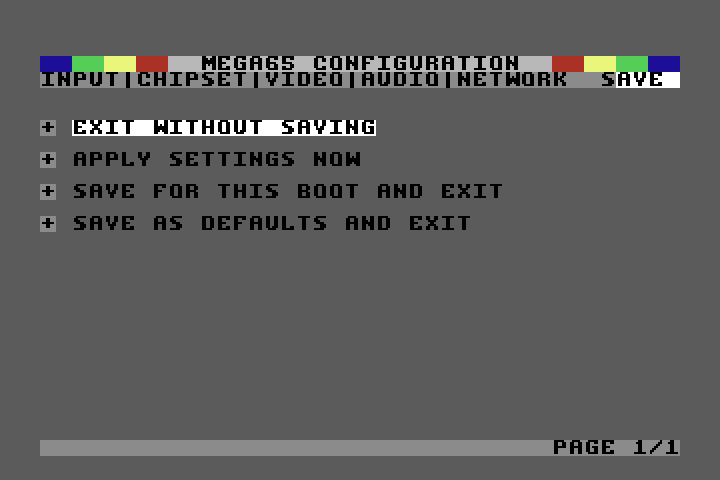
\includegraphics[width=\linewidth]{images/ss-m65config-save.png}

\begin{itemize}
  \item{\em Exit Without Saving} allows you to abandon any changes
    made in the MEGA65 Configure utility, without saving them.
  \item{\em Apply and Test Settings Now} makes the settings take
    immediate effect.  This can be helpful for testing compatibility
    of your TV or monitor with PAL or NTSC video modes.  If you
    still see your display after applying such a change,
    it is safe to save those settings.
  \item{\em Restore Factory Defaults} allows you to reset the
    MEGA65 configuration settings to the factory defaults. It also
    randomly selects a new MAC address for models that include an
    internal Ethernet adaptor.  If you wish to commit these
    changes, you must still save them.
  \item{\em Save as Default and Exit} commits any changes you
    have made to the SD card storage, so that they will be used
    whenever your MEGA65 is turned on.
\end{itemize}

\subsection{Input Devices}

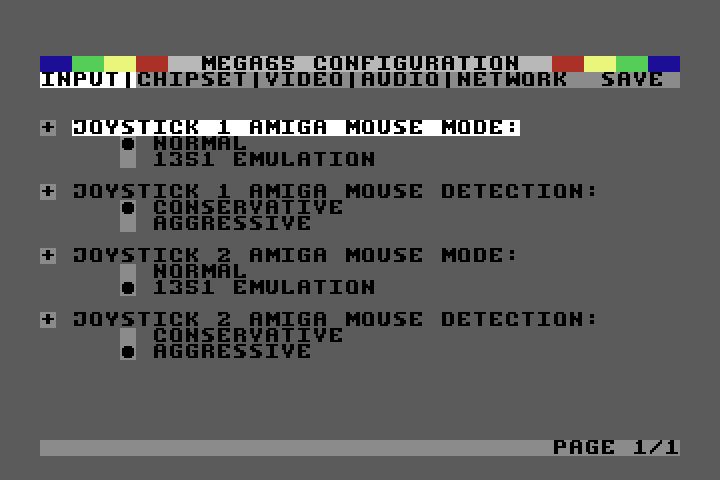
\includegraphics[width=\linewidth]{images/ss-m65config-1.png}

\begin{itemize}
  \item{\em Joystick 1 Amiga Mouse Mode} allows either {\bf normal} operation,
    where software will see it as an Amiga mouse, or {\bf 1351
      emulation} mode, where the MEGA65 translates the Amiga mouse's
    movements into 1351 compatible signals. This allows you to use an
    Amiga mouse with existing C64/C65 software that expect a 1351
    mouse.
  \item{\em Joystick 1 Amiga Mouse Detection} can be set to conservative
    or aggressive.  If you use an Amiga mouse, and it fails to move
    smoothly in all directions, you may set it to {\bf
      aggressive}. Conversely, if you regularly use joysticks in the
    port, and have difficulties with the joystick input
    mis-behaving, you may select the {\bf conservative}
    option.
  \item{\em Joystick 2 Amiga Mouse Mode} is the same as the first
    option, but for the second joystick port. This allows you to
    have different policies for each port.
  \item{\em Joystick 2 Amiga Mouse Detection} similarly provides the
    ability to separately control the Amiga mouse detection
    algorithm for the second joystick port.
\end{itemize}


\subsection{Chipset}

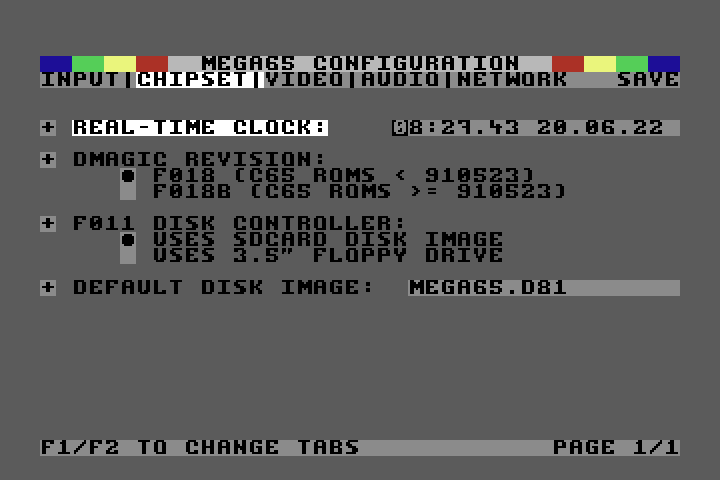
\includegraphics[width=\linewidth]{images/ss-m65config-2.png}

\begin{itemize}
  \item{em Real-Time Clock} allows setting the MEGA65's Real-Time
    Clock for those models that include one.  To set the clock or
    calendar, simply edit the field and press the \specialkey{RETURN}
    key.  The display does not change while viewing this page, but if
    you use the cursor left and right keys to select another page and
    return to this page, the values will update if a Real-Time Clock
    is fitted and functioning.
  \item{\em DMAgic Revision} allows selecting the default mode of
    operation for the C65 DMAgic DMA controller.  This option is only
    required for ROMs not detected by the MEGA65's HYPPO Hypervisor.
    If you see screen corruption in BASIC,
    try toggling this option.
  \item{\em F011 Disk Controller}
    This option allows you to select whether the internal 3.5'' floppy
    drive functions using real diskettes, or whether it simply makes
    noises to add atmosphere when using D81 disk images from the SD
    card.  This merely sets the default option, and you can change
    this setting, or select a different disk image for use as either
    or both of the C65 3.5'' DOS based drives.
  \item{\em Default Disk Image} allows you to choose the D81 disk image
    used with the internal drive, if the F011 Disk
    Controller option above is set to use an SD card disk image.    
\end{itemize}

\subsection{Video}

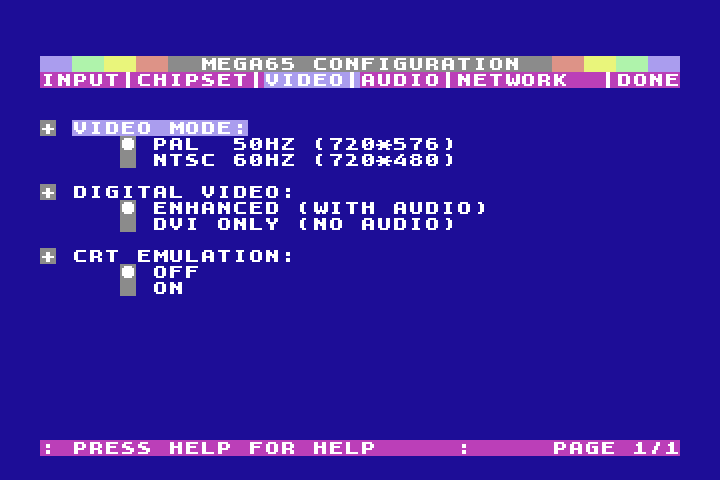
\includegraphics[width=\linewidth]{images/ss-m65config-3.png}

\begin{itemize}
  \item{\em Video Mode} selects whether the MEGA65 starts in PAL or NTSC.
    The MEGA65 supports true 480p NTSC and 576p PAL double-scan modes,
    with exact 60Hz / 50Hz frame-rates.  This setting sets the
    default value, and the system can be switched between PAL and NTSC
    via the Freeze Menu, or under software control by MEGA65-enabled
    programmes.
\end{itemize}

\subsection{Audio}

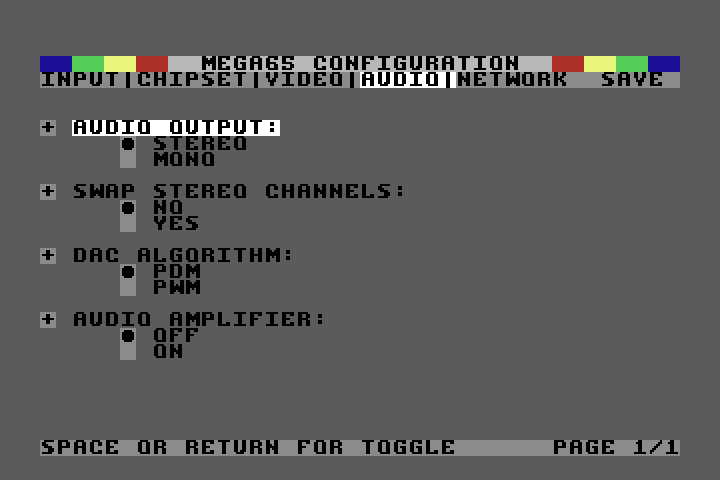
\includegraphics[width=\linewidth]{images/ss-m65config-4.png}

\begin{itemize}
  \item{\em Audio Output} selects whether the SIDs and digital audio
    channels are combined to provide a mono-aural signal, or whether
    the left and right tagged audio sources are separated to provide a
    stereo signal. Again, this setting can be varied from in the Audio
    Mixer of the Freeze Menu, or under the control of MEGA65-enabled
    software.
  \item{\em Swap Stereo Channels} allows switching the left and right
    sides of the stereo audio output. This is primarily useful for
    software that expects left and right SIDs to be at swapped
    addresses compared with the MEGA65.
  \item{\em DAC Algorithm} allows selecting between two different
    digital to analog conversion algorithms.  Both are very good,
    but you may have a preference for one or the other.
  \item{\em Audio Amplifier} allows enabling or disabling the audio
    amplifier contained in some models of the MEGA65 for
    certain audio outputs, e.g., internal speaker or loud speaker.
\end{itemize}

\subsection{Network}

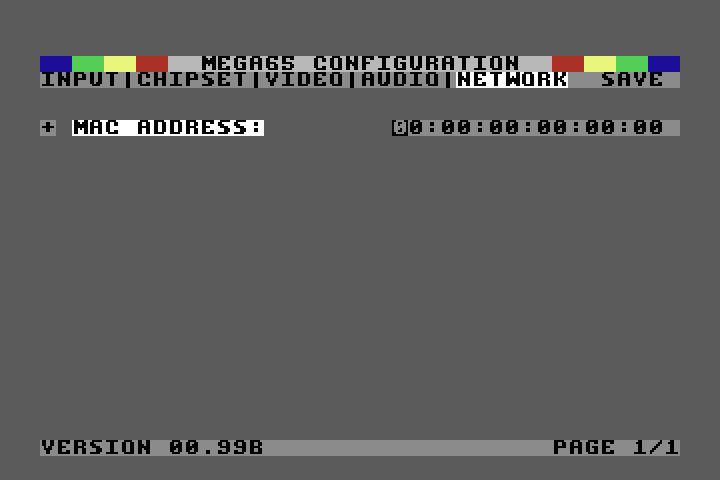
\includegraphics[width=\linewidth]{images/ss-m65config-5.png}

\begin{itemize}
  \item{\em MAC Address} allows you to set the default MAC address of your
    MEGA65.  This can be changed at run-time by MEGA65-enabled
    software
\end{itemize}

\chapter{Cores and Flashing}
\label{cha:cores}

\phantomsection
\section{What are cores, and why do they matter?}

The MEGA65 computer uses a versatile chip called an FPGA as its heart, which is
an acronym for ``Field Programmable Gate Array''. This is a fancy way of
saying that FPGAs are chips that can be programmed {\it by you} to impersonate
other chips. They do this by re-configuring their arrays of logic gates to
reproduce the circuits of other chips. As a result, FPGAs are not an emulation,
but a re-creation of other chips.

However, FPGAs forget what chip they are pretending
to be whenever the power is turned off, or when they are re-programmed.
This might sound annoying, but it's actually very powerful. It means that
you can tell the FPGA in the MEGA65 to impersonate not just the MEGA65 design
as it currently stands, but to impersonate any improvements made to the design itself.
In other words, you can upgrade the MEGA65 hardware just by providing a new
set of instructions to the FPGA.  These sets of instructions are called ``cores'',
or ``bitstreams''. For the purpose of the MEGA65, these two terms are interchangeable.

FPGAs are so flexible that not only is it possible to teach the MEGA65 to be a better
MEGA65, but it is also possible to teach the MEGA65 to be other interesting
home computers. We believe that the FPGA is powerful enough to re-create
a Commodore PET\texttrademark, VIC-20\texttrademark, Apple II\texttrademark, Spectrum\texttrademark,
BBC Micro\texttrademark, or even an Amiga\texttrademark, or one of the 16-bit era game consoles. Unlike some
previous FPGA-based retro-computers, the MEGA65, its FPGA instructions, board layout, and other information is
all available for free under various open-source licenses. This means that anyone is free to
create other cores for the MEGA65 hardware.

To top it all off, the MEGA65 has enough storage for 7 different sets of FPGA instructions,
so that you can easily switch the MEGA65's ``personality'' from being a MEGA65 to another
system, and back again.

The remainder of this chapter describes how to select a core to run on the MEGA65, and
how to store a core into one of the seven slots in the flash memory storage.

\ifdefined\printmanual
% no need for model types to be in the user guide?
\else
  \subsection{Model types}
  Retail models of the MEGA65 are referred to as the MEGA65R3A (revision 3A). Throughout the course of development of the MEGA65, there have been several other model variants used by developers, each with differing specifications and available core slots, so they will be listed here, just to raise awareness of them.

  \begin{minipage}{\linewidth}
    \begin{center}
      \begin{longtable}{|C{2.5cm}|C{2cm}|C{2cm}|C{2cm}|C{2cm}|}
        \hhline{|=|=|=|=|=|}
        {\textbf{Model}} & {\textbf{FPGA type}} & {\textbf{QSPI size}} & {\textbf{\#slots}} & {\textbf{slot size}} \\
        \hhline{|=|=|=|=|=|}
        \multirow{2}{*}{\textbf{MEGA65R3A}} & \multicolumn{4}{l|}{The retail/release version of the MEGA65} \\
        \cline{2-5}
        & A200T & 64MB & 8 & 8MB \\
        \hhline{|=|=|=|=|=|}
        \multirow{2}{*}{\textbf{MEGA65R3}} & \multicolumn{4}{l|}{The DevKit model} \\
        \cline{2-5}
        & A200T & 32MB & 4 & 8MB \\
        \hhline{|=|=|=|=|=|}
        \multirow{2}{*}{\textbf{MEGA65R2}} & \multicolumn{4}{l|}{An earlier MEGA65 model} \\
        \cline{2-5}
        & A100T & 32MB & 8 & 4MB \\
        \hhline{|=|=|=|=|=|}
        \multirow{2}{*}{\textbf{Nexys4}} & \multicolumn{4}{l|}{FPGA development boards used early in the project} \\
        \cline{2-5}
        & A100T & 16MB & 4 & 4MB \\
        \hline
      \end{longtable}
    \end{center}
  \end{minipage}
\fi


\section{Bitstream files}
\label{sec:bitstreamfiles}

Firstly, there are a variety of files related to the MEGA65's cores/bitstreams that you should be familiar with, in
order to decide what file-types are needed for what occasion.

\subsection{File types}

\index{.bit files}\index{.mcs files}\index{.prm files}\index{.cor files}
\begin{center}
  \begin{longtable}{|L{1.5cm}|p{10cm}|}
    \hline
    {\textbf{File-type}} & {\textbf{Purpose}} \\
    \hline
    {\tt .cor} & {The MEGA65 project's custom bitstream file format, containing extra header information to help identify the bitstream and the specific MEGA65 target device it is intended for. The MEGA65's flashing utility makes use of this additional information to ensure you don't accidentally flash the bitstream of a different device.} \\
    \hline
    {\tt .mcs} & {The bitstream file in a format needed when flashing it to your device's QSPI flash memory chip via Vivado\textregistered.} \\
    \hline
    {\tt .prm} & {This file contains checksum information that can be used by Vivado to verify the {\tt .mcs} file you have tried to flash. Optional.} \\
    \hline
    {\tt .bit} & {A plain bitstream file that can be copied to your SD card.} \\
    \hline
  \end{longtable}
\end{center}

\subsection{Where to download}

Visit the following url:

\url{https://files.mega65.org}

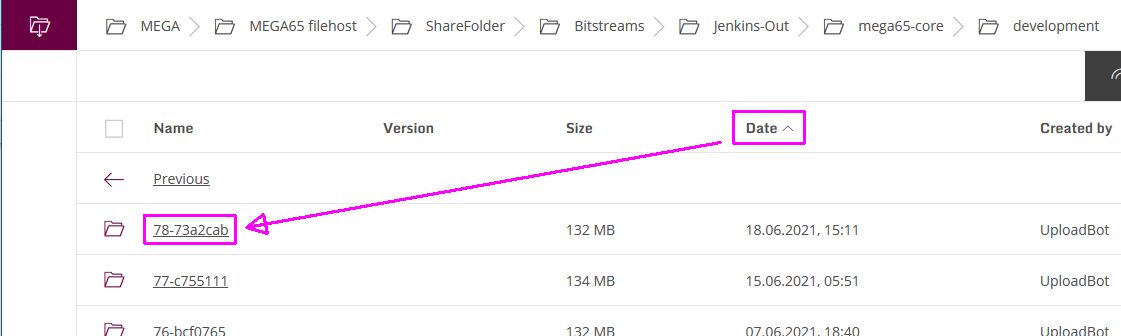
\includegraphics[width=\linewidth]{images/latest_bitstream.png}

Click the {\bf Files} tab, and in the search-bar, type {\bf .cor} and press Enter.
\ifdefined\printmanual
  You will notice that there are different files with the {\tt .cor} extension. For your MEGA65, download the file
  that ends with {\bf 65r3-dev.cor}. Other files are for other device types, which you can read more about in the
  {\bf MEGA65 Book}.
\else
  For the purposes of this chapter on core-flashing, download the desired .cor file that suits your target device:

  \begin{itemize}
    \item{\textbf{mega65r3-dev.cor} (for MEGA65R3 boards, both Release and DevKits)}
    \item{\textbf{mega65r2-dev.cor} (for MEGA65R2 boards)}
    \item{\textbf{nexys4ddr-widget-dev.cor} (for Nexys4 DDR boards)}
    \item{\textbf{nexys4-dev.cor} (for Nexys4 PSRAM boards)}
    \item{You can also find .bit, .mcs and .prm files located here too.}
  \end{itemize}

  Alternatively, if you intend to flash the QSPI chip via Vivado, you would instead download the .mcs file for your target device (and optionally, the .prm files as well).

  Another alternative for Nexys4 board users is to download .bit files and copy them to SD cards, which you can also download.

  But once again, for the purposes of this chapter on core-flashing, you will only be interested in the .cor files.
\fi

\phantomsection
\section{Selecting a core}

To operate the MEGA65 with an alternate core, switch off the power to the MEGA65, and then hold
\specialkey{NO SCROLL} down while switching the power back on. This instructs the MEGA65 to enter the
Flash and Core Menu, instead of booting normally. When booting this way, the following screen will appear:

\begin{center}
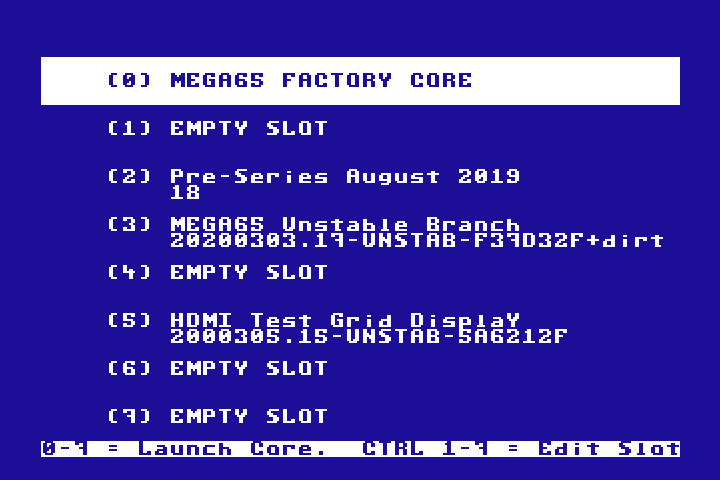
\includegraphics[trim= 0  0 0 10mm,clip,width=0.7\linewidth]{images/ss-flashmenu.png}
\end{center}

To select a core and start it, use the cursor keys to highlight the desired core, and then press
\specialkey{RETURN}.  If you select a flash slot that does not
contain a valid core, it will be highlighted in red to indicate that it
cannot be booted from:

\begin{center}
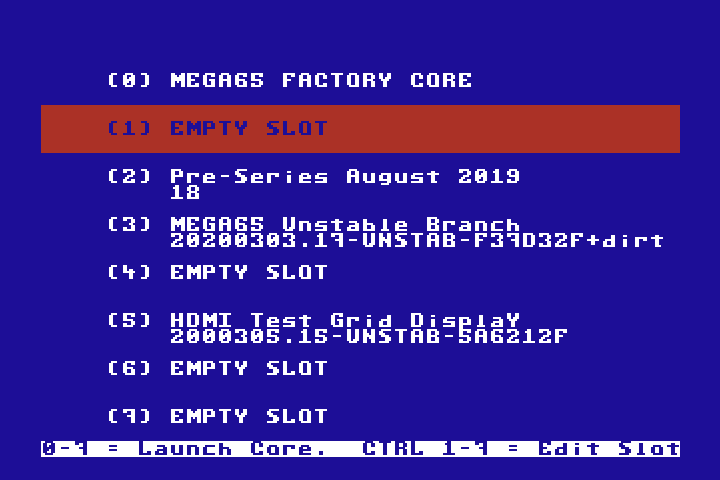
\includegraphics[trim= 0  0 0 10mm,clip,width=0.7\linewidth]{images/ss-flashmenu-invalidslot.png}
\end{center}

Alternatively, you can press the number corresponding to the core you would
like to use. The MEGA65 immediately reconfigures the FPGA, and launches the core.  If for some reason
the core is faulty, the MEGA65 may instead restart normally after a few seconds, and depending on the
circumstances, take you back into the menu automatically.

The MEGA65 will keep running the new core until you physically power it off.  Pressing the reset button
will not reset which core is being run.

\phantomsection
\section{Installing an upgrade core for the MEGA65}

Installing and upgrading the core (from a {\tt .cor} file) for the MEGA65 can be done in a few easy steps.

First, copy the core onto the MEGA65's SD card. You can do this by removing the SD card and copying a previously
downloaded core file to it from another computer. Alternatively,
you can insert an SD card that already contains the upgrade core. Finally, you can use the MEGA65 TFTP Server
program and the MEGA65's Ethernet port to upload the core upgrade file onto the SD card from another computer
on your local network.

The Flash Menu will use the external microSD slot over
the internal SD card, so if you have both a microSD card and SD card
inserted in your MEGA65, the Flash Menu will ignore the
internal SD card. To avoid this, simply copy the core(s) from the internal SD
card to the external microSD card, or temporarily remove the external
microSD card from the rear of your MEGA65, so that the Flash Menu will
be able to find the core files.  Also note that the Flash Menu
currently only supports DOS-style 8.3 character filenames in UPPERCASE. If your
core files have a longer name, you will need to rename them when
copying them onto your microSD or SD card.

Next, once you have the upgrade core on the MEGA65's SD card, enter the Flash and Core Menu as above,
i.e., switch off the power, and hold \specialkey{NO SCROLL} down while switching the power on again.  When the Flash
and Core Menu appears, hold \specialkey{CTRL} down and press
\megakey{1} (or \specialkey{CTRL} and a different number, if you wish to replace the
contents of a different flash slot). The MEGA65
will present you with a list of core files that are on the SD card:

\begin{center}
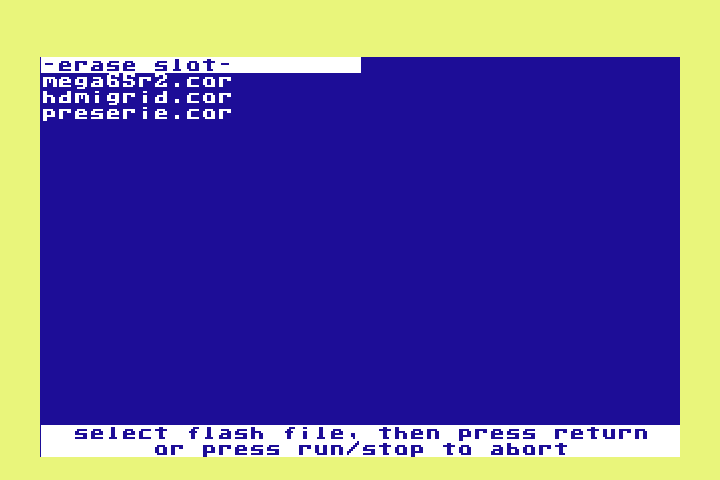
\includegraphics[trim= 10mm  5mm 10mm 15mm,clip,width=0.7\linewidth]{images/ss-flashmenu-selectcore.png}
\end{center}

Select the upgrade core file you wish to
install using the cursor keys, and then press \specialkey{RETURN}.  The MEGA65 will then erase
the flash slot, before writing the upgraded core.  You will see a progress bar while the MEGA65 erases
the flash slot:

\begin{center}
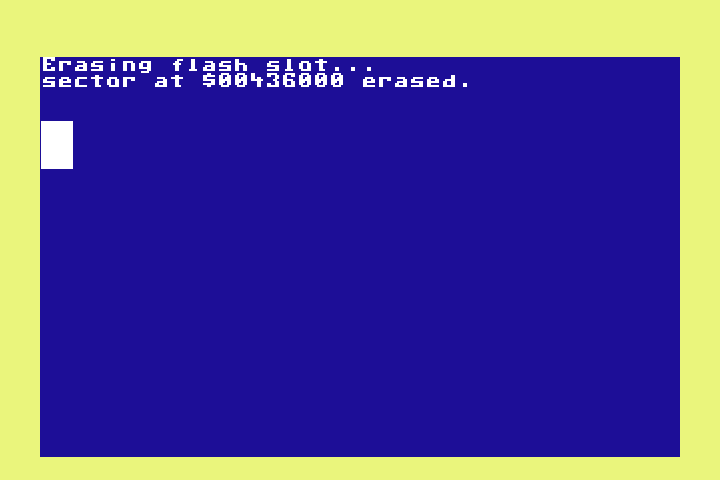
\includegraphics[trim= 10mm  3mm 10mm 15mm,clip,width=0.7\linewidth]{images/ss-flashmenu-erasing.png}
\end{center}

The progress bar will then reset, and the MEGA65 will
write the new core into the slot. This process can take up to 15
minutes, depending on the size of the core file.  If you simply wish
to erase a flash slot, you can select the
\screentext{-- erase slot --} option instead of a file name. This will then perform
only the erasure part of the process.

{\bf It is important to not switch the power off during this process}. If you do, the core file will be
only partially installed, and the MEGA65 may not start properly.
While
inconvenient, it won't damage your MEGA65 or leave it
in an unusable state: It will simply fall back to using the factory
supplied core.
If this happens, enter the Flash and Core Menu
as described above, and follow the instructions again.

When the flashing process has completed, you will see a message indicating that the process is complete:

\begin{center}
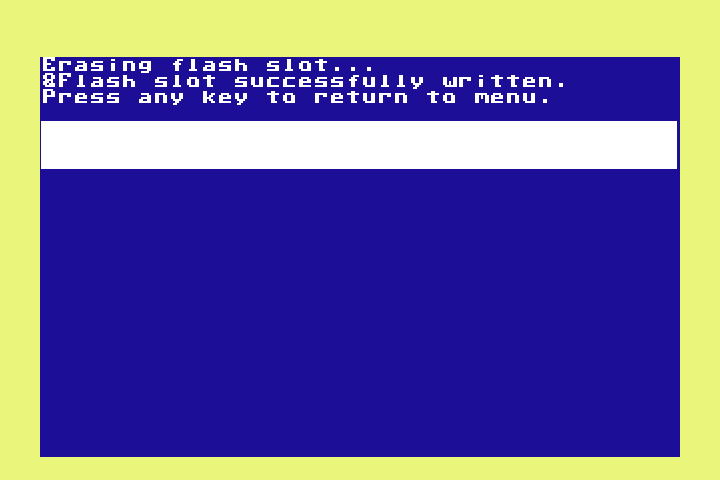
\includegraphics[trim= 10mm  3mm 10mm 15mm,clip,width=0.7\linewidth]{images/ss-flashmenu-done.png}
\end{center}


When this happens, simply switch off the power to the MEGA65 and switch it back on again for it to start using the
upgraded core.  This is because the MEGA65 will always try to start the core in slot 1 when
it is switched on.

\phantomsection
\section{Installing other cores}

Installing other cores works very similarly to installing upgrade cores. The only difference is that you
press \specialkey{CTRL} and \megakey{2} to \megakey{7} from the Flash and Core Menu, so that the core
gets installed to another slot.

Of course, there is nothing stopping you from installing a different core
in slot 1, so that the MEGA65 behaves as a different type of computer when you switch it on.  If you do this,
you can always choose to run the MEGA65 core by entering the Flash and Core Menu, and selecting the MEGA65
core.

\phantomsection
\section{Creating cores for the MEGA65}

If you would like to create your own cores for the MEGA65, or help
contribute to the MEGA65 core, then
you may also wish to take a look at
\ifdefined\printmanual
the {\bf MEGA65 Book},
\else
\bookvref{cha:fpgacpldflashing},
\fi
which explains how to use the
FPGA development tools to flash the MEGA65.

\phantomsection
\section{Replacing the factory core in slot 0}

Replacing the core in slot 0 is not recommended, because if it ever gets corrupted, it will ``brick'' the machine.
This will require you to connect a TE-0790 JTAG programmer, by opening your MEGA65 case, installing
the module, going through some rather convoluted software preparation steps (similar to if you were
creating your own bistream/core) and then restoring a working bitstream into the slot.

The MEGA65 is an open system though, so it's possible for you to do all of this, but it's very hard. There
is a secret key-press combination in the Flash Menu that will then challenge you with a series of questions with
increasing difficulty to ensure that you know what you are doing. Only after you have correctly
answered these questions will you be given the option to erase and/or replace the contents of slot 0.
Details of the questions asked are purposely not documented.

There really should be no reason for using this method to replace the contents of slot 0:
If you want to make your own bitstreams/cores, you can either write them to other slots and use the
Flash Menu to activate them, or you can simply use a TE-0790 JTAG programmer, and then use
Vivado or other FPGA development tool to write to the flash directly. This method is also
somewhat faster than flashing through the Flash Menu.

{\bf You have been warned!}

\phantomsection
\section{Understanding The Core Booting Process}

This section summarises how the MEGA65 selects which core to start with when it is switched on.
The process is shown in the following figure:

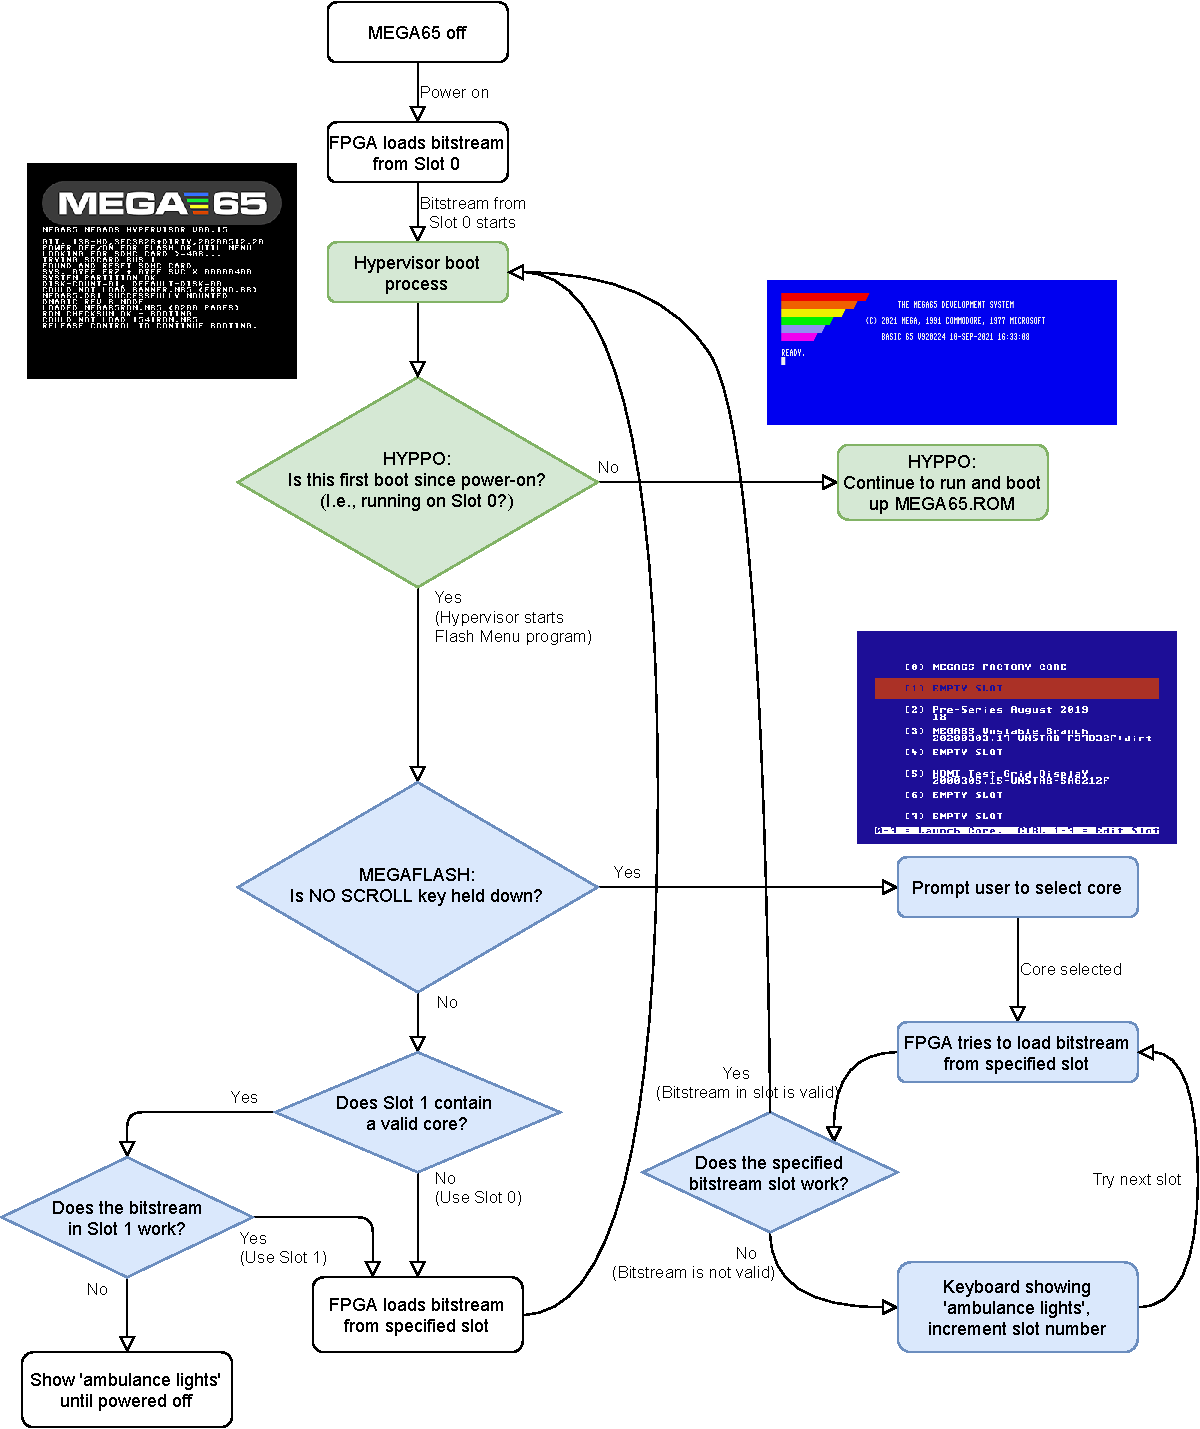
\includegraphics[width=\linewidth]{images/illustrations/flashmenu-flowchart.pdf}

The booting process is governed by two facilities:
\begin{itemize}
  \item The Hypervisor (also known as HYPPO), which operates at a level above the Kernal. One of its responsibilities is to manage aspects of the boot process. For more details on the Hypervisor, refer to  
\ifdefined\printmanual
the {\bf MEGA65 Book}.
\else
 \bookvref{sec:hypervisor-mode}.
\fi
    In the diagram, activities performed by the Hypervisor have been highlighted in green.
  \item The Flash Menu program (also known as MegaFlash), which provides a list of available core slots to choose from. In the diagram, activities performed by MegaFlash have been highlighted in blue.
\end{itemize}

When the MEGA65 is switched on, it does the following:
\begin{itemize}
\item Loads the bitstream stored in slot 0 of flash memory. If that is the MEGA65 Factory Core, the MEGA65 
  HYPPO Hypervisor starts.
\item If it is the first boot since power-on (which implies that we are running from slot 0), HYPPO starts the Flash Menu program (aka MegaFlash) -- but note that the Flash Menu in
      this mode may not show anything on the screen to indicate that it is running!
\item The Flash Menu then checks if \specialkey{NO SCROLL} is being held down.
\item If it is, the Flash Menu program shows its display, allowing you to select or re-flash a core.
\item If \specialkey{NO SCROLL} is \underline{not} being held down, the Flash Menu program checks if Flash Slot 1 contains a valid
      core.
\item If it does, then the Flash Menu program attempts to load that core.
\item If it succeeds, then the system reconfigures itself for that core, after which the behaviour of the system is
      according to that core.
\item If it fails, the keyboard will go into ``ambulance mode'', showing flashing blue lights to indicate that some
      first-aid is required. Note that in ambulance mode the reset button has no effect: You must switch the
      MEGA65 off and on again.
\end{itemize}



If you have selected a different core in the Flash Menu, the process
is similar, except that the ambulance lights will appear for only a
limited time, as the FPGA will automatically search through the flash
memory until it finds a valid core. If it gets to the end of the flash
memory, it will start the MEGA65 Factory Core from slot 0 again.





\chapter{Floppy Disks, D81 Images, and the Freezer}
\label{cha:freezer}

\phantomsection

\section{Disk Drives}
The MEGA65 is compatible with a wide range of floppy disk drives, and can be configured to use them in a variety
of different ways. It includes an internal 3.5" drive, which is compatible with double density and high density
3.5" disks. But did you know you can also use 5.25" disks? By connecting a compatible IEC drive to the rear
Floppy Disk Drive/IEC Connector, you can use your MEGA65 with two or more physical floppy drives simultaneously!

There are also IEC drive emulators available, such as the SD2IEC. These devices
(and the MEGA65) use ``disk images'', which are files that represent a floppy disk, usually stored on an SD card.
By ``mounting'' a disk image file to a disk drive emulator, the MEGA65 can then use these files without realising it's
actually being emulated. As far as the MEGA65 is concerned, it's using a real drive.

This allows you to use modern media to read and write your programs, and in some cases can drastically reduce
read and write times. These files usually have the extension {\bf .d64} (named after the C64), which are files that
represent a {\it single} side of a 5.25" disk, or {\bf .d81}, which represents an entire 3.5" disk (named after the
1581 floppy disk drive).

The MEGA65 can use either real disks and drives, {\bf .d81} files, or a combination of both.

\subsection{Disk Drive Terminology}
Before you get to know how to use the various disk drives that work with the MEGA65, it's important to be aware
of some specific terminology which CBM computers and the MEGA65 use. This includes {\bf BASIC} commands (such as
{\bf LOAD} and {\bf SAVE}), and {\bf CBDOS} (Computer Based Disk Operating System), which use the following:

{\bf UNIT} is a device number in the range of 0-31.
The numbers from 0 to 11 are reserved for the following device types:

\setlength{\tabcolsep}{1mm}
\begin{center}
\begin{tabular}{|l|l|l|}
\hline
{\bf Unit} \# & {\bf Device}  & {\bf Notes} \\
\hline
0        & Keyboard & Input \\
1        & Unused   & Was used for Cassettes on the C64 \\
2        & Unused   & Was used for RS-232 on the C64 \\
3        & Screen   & Input/Output     \\
4-5      & IEC Printer  & Output     \\
6-7      & IEC Plotter  & Output     \\
8-9      & CBDOS drives\footnotemark{} & Internal floppy drive, 1565\footnotemark{}, or disk image \\
10-11    & IEC drives   & 1541, 1571, 1581, FD-2000 \\
\hline
\end{tabular}
\end{center}
\addtocounter{footnote}{-2}
\stepcounter{footnote}\footnotetext{IEC drives can be assigned to devices 8-9, by moving the built-in MEGA65 devices
                                    to 10-11 first. Once the drives have been reassigned, the IEC drives can be
                                    powered on.}
\stepcounter{footnote}\footnotetext{The 1565 was a prototype external C65 disk drive that never made it to production.}

{\bf DRIVE} is the drive number of a {\bf UNIT}:

\setlength{\tabcolsep}{1mm}
\begin{center}
\begin{tabular}{|l|l|l|}
\hline
{\bf Unit}  & {\bf Drive Numbers} & {\bf Comment} \\
\hline
1541 IEC & 0             & Single drive \\
1571 IEC & 0             & Single drive \\
1581 IEC & 0             & Single drive \\
FD-2000 IEC & 0             & Single drive (CMD)\\
FD-4000 IEC & 0             & Single drive (CMD)\\
SD2IEC      & 0             & Disk images\\
4040 IEEE-488 & 0,1             & Dual drive (CMD)\\
8050 IEEE-488 & 0,1             & Dual drive (CMD)\\
8250 IEEE-488 & 0,1             & Dual drive (CMD)\\
\hline
\end{tabular}
\end{center}
% thw following few paragraphs probably needs more wording. Sounds like a list of bullet points which isn't pretty.
For all single drives, the drive number is always 0.
This includes all of the well known drives with an IEC interface.

Dual disk drives (which use drive numbers 0 and 1) are usually equipped with an IEEE-488 interface, and need
an IEEE-488 to IEC converter to be used on the MEGA65.

The internal floppy controller of the MEGA65 can be used to control
two floppy drives. However, both drives must be attached to the same ribbon cable.

{\bf BASIC} commands that address files or disks include
{\bf U} for UNIT and {\bf D} for drive, which use the default values of
{\bf UNIT = 8}, and {\bf DRIVE = 0}.

\section{The Freezer}
The MEGA65 {\bf FREEZER} is a tool for changing system parameters at any time,
regardless of the currently running program. It's very similar to the Freezer that many popular cartridges
for the C64 included, such as the Action Replay cartridge, and The Final cartridge. Freezers generally work by
taking over the CPU whilst leaving RAM intact. This way you can perform functions and change configuration
settings without affecting the currently running program. Once you have finished using the Freezer, CPU control
is given back to the original program.


The Freezer is invoked by pressing \widekey{RESTORE} for approximately half to one second.
The current status of the computer is frozen and the Freezer menu,
similar to the picture below is displayed. This chapter focuses on how to assign disk images and how to configure the
the internal floppy disk drive, but the other options in the Freezer are self explanatory, or will be covered in detail in
online documentation.

\begin{center}
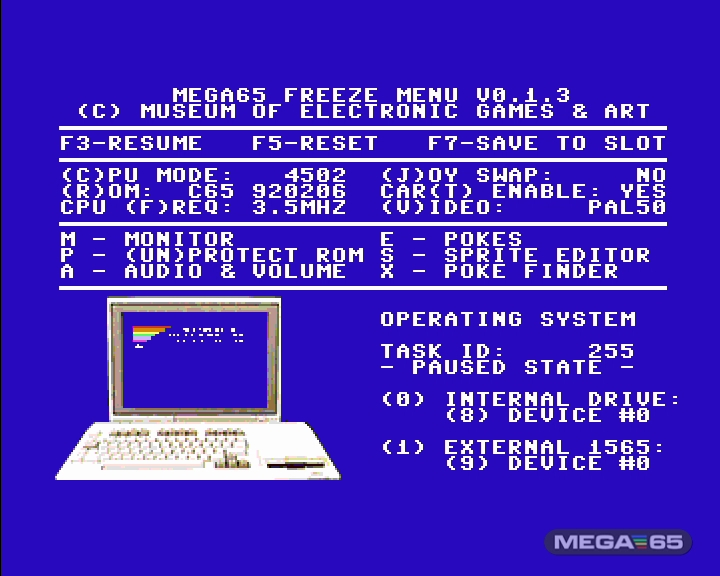
\includegraphics[trim= 10mm 20mm 10mm 20mm,clip,width=0.7\linewidth]{images/freezer.jpg}
\end{center}

The bottom-right part of the Freezer screen shows the current disk drive assignments.
The internal CBDOS which the MEGA65 uses supports up to two
3.5" disk drives and .d81 images, in any combination.
Drive 0 can be assigned to the internal floppy disk drive or a .d81 disk image,
whereas Drive 1 can be assigned to an external floppy disk drive (connected to the
same ribbon cable as the internal drive), or a .d81 disk image.

A typical configuration is usually one of the following:
\begin{center}
\begin{tabular}{|l|l|l|}
\hline
{\bf Drive 0 Assignment} & {\bf Drive 1 Assignment} \\
\hline
Internal floppy disk drive &  Disk image \\
Disk image                 &  Disk image \\
\hline
\end{tabular}
\end{center}

The assignment, and mounting of disk images can be performed by pressing
\megakey{0} for drive 0, or \megakey{1} for drive 1.

You may have noticed that the drive numbers here (0-1) are different to the more commonly used {\bf UNIT}
numbers (8-9), which you may be more used to. The drive numbers of 0 and 1 are used internally by CBDOS.
However, {\bf BASIC} and Kernal address these storage devices by {\bf UNIT} numbers. CBDOS emulates two single drives for
the operating system, by assigning separate unit numbers to drive 0 and drive 1.
The default assignment is:

\begin{center}
\begin{tabular}{|l|l|l|}
\hline
{\bf Unit/Drive} & {\bf Assignment} \\
\hline
UNIT 8, DRIVE 0  & Internal drive 0 (internal floppy or disk image) \\
UNIT 9, DRIVE 0 & Internal drive 1 (external floppy or disk image) \\
\hline
\end{tabular}
\end{center}


You may wish to change this unit assignment, if for example
a 1541 drive is connected to the IEC port as unit 8.
In this case, the internal drive assignment can be switched to an alternative unit
to avoid conflict. To do this, press \megakey{8} to toggle the unit assignment of drive 0
between 8 and 10, and \megakey{9} to toggle the unit assignment of drive 1, between 9 and 11.

After setting the preferences, the Freezer can be exited
with \megakey{F3}. The Freezer restores the screen and
returns to the interrupted program.

Note: The drive and unit assignments are temporary, and will be reset to their defaults
after power down or reset. For permanent settings, use the {\bf CONFIGURE}
menu. You can read more about this menu on page \pageref{configuring-chipset}.

\section{Using D81 images}
As previously mentioned, the MEGA65 allows the use of D81 files instead of using physical disks. The MEGA65 includes a
built-in file browser, which allows you to choose which D81 file to mount. To do this, enter the Freezer menu,
then press \megakey{0} or \megakey{1}, to choose the drive to mount it to.

When you do this, the file browser will appear:

\begin{center}
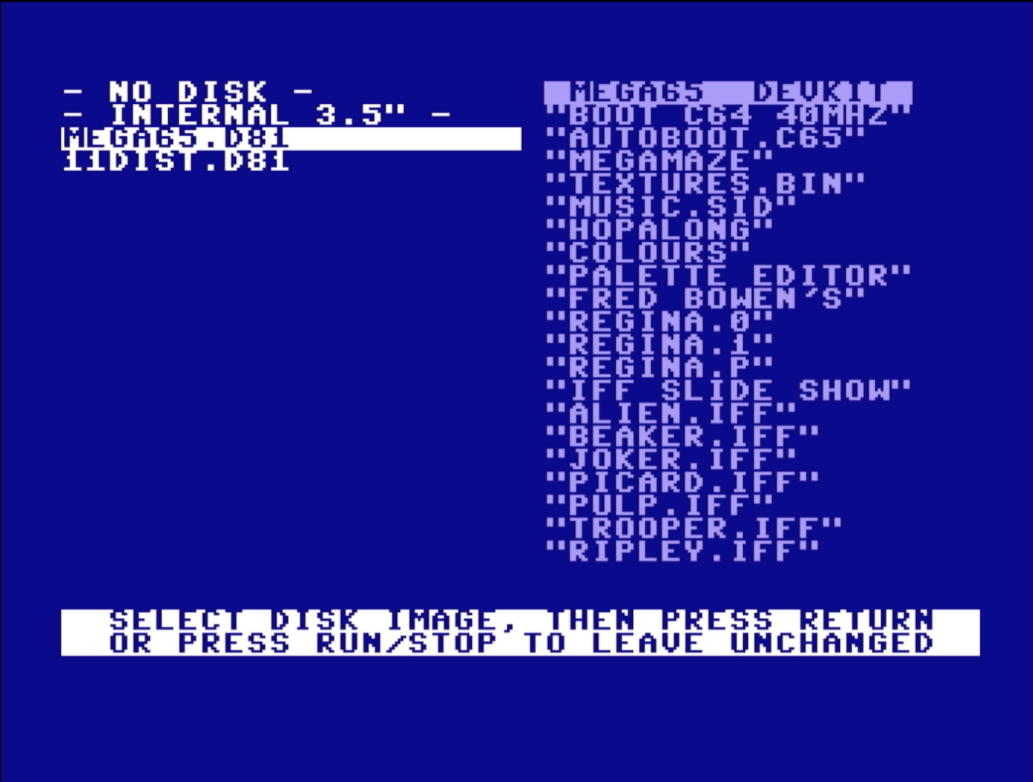
\includegraphics[trim= 10mm 20mm 10mm 20mm,clip,width=0.7\linewidth]{images/d81-file-browser.png}
\end{center}

The file browser will list all D81 images on the microSD card. The MEGA65 prioritises the microSD card, so if you
prefer to use an image on the internal SD card, the microSD card should be removed (when doing this, the MEGA65 needs
to be reset as well).

Press the cursor keys to choose a file. If the currently selected file isn't a valid D81, the border will be red,
otherwise it will be blue, as shown above. Whilst browsing for D81 files, the list of files within the currently
selected D81 file will be shown on the right-hand side.

When you find the D81 file you wish to mount, press \specialkey{RETURN}.
This will take you back to the Freezer menu, and the selected D81 file will be shown under the selected drive.
In the screenshot below, the  \screentext{MEGA65.D81} file has been mounted to drive 0:

\begin{center}
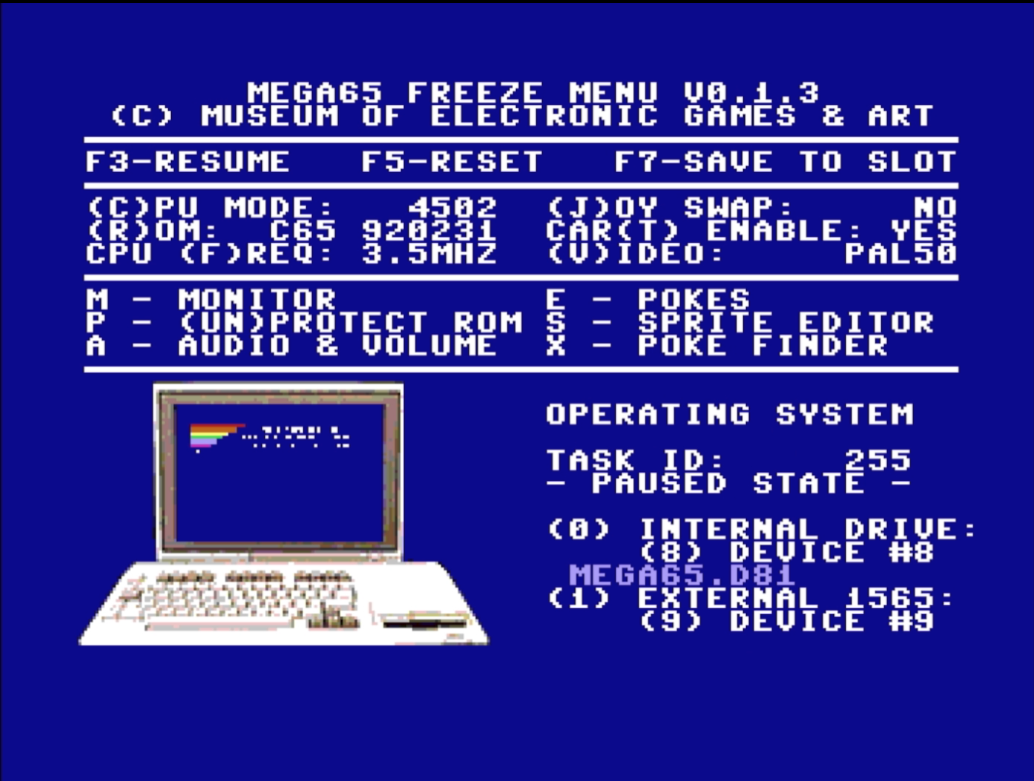
\includegraphics[trim= 10mm 20mm 10mm 20mm,clip,width=0.7\linewidth]{images/freezer-chosen-d81.png}
\end{center}

Next, press \megakey{F3} to exit the Freezer menu and return to the currently running program. Alternatively,
pressing \megakey{F5} will exit the Freezer, and reset the MEGA65 as well.

Now that the file has been mounted, you can use
the {\bf DIR} command to list the files in the image, or any of the {\bf LOAD}, and {\bf SAVE} commands, like you
would on a physical disk.


\subsection{Auto booting from a D81 file}
If you would like the MEGA65 to automatically perform any BASIC commands upon startup, you can create an
\screentext{AUTOBOOT.C65} PRG file on your disk image. In this file, you can write BASIC programs to do things such
as changing the {\bf BACKGROUND}, {\bf BORDER}, or {\bf FOREGROUND} colours, or even {\bf LOAD} a program.

For example, to change the background and border colours to black, and load a program called \screentext{MYPROGRAM}
automatically, create a BASIC listing like the following, then {\bf SAVE} it.


\begin{tcolorbox}[colback=black,coltext=white]
\verbatimfont{\codefont}
\begin{verbatim}
10 BACKGROUND 0
20 BORDER 0
30 LOAD "MYPROGRAM.PRG"
SAVE "AUTOBOOT.C65"
\end{verbatim}
\end{tcolorbox}


\part{FIRST STEPS IN CODING}

\chapter{How Computers Work}

Did you know that many computer experts and programmers learned how to
use computers when they were still small children?
Home computers only became common in the early 1980s. They were so new,
that people would often write programs to do
what they wanted to do, because no software existed to do the job for them.

It was also quite common for people working in all
sorts of office jobs to learn how to program the computers they used for
their jobs.  For example, the people processing payroll
for a company would often learn how to program the computer to calculate
the everyone's pay!

Things have changed a lot since then, though.
Now most people choose existing programs or apps to do what they need,
and think that programming is a specialised skill that only some people
have the ability to learn.
But this isn't true.  Of course, like every other field of pursuit
everyone will be better at some things than others,
whether it be sports, knitting, maths or writing. But almost
everyone is able to learn enough to help them in their life.

We created the MEGA65, because we believe that YOU can learn to
program, so that computers can be more useful to you, and as with
learning any new skill, that you can have the satisfaction and enjoyment
and new adventures that this brings!


\phantomsection
\section{Computers are stupid. Really stupid}

How can this be so? Computers are able to do so many different things, often thousands of times faster than a person can.
So how can we say that computers are stupid?  The answer is that no computer can do anything that it hasn't been instructed
by a person to do.  Even the latest Artificial Intelligence systems were instructed how to learn (or how to learn, how to learn).
To understand why this is so, it is helpful to understand how computers really work.

\subsection{Making an Egg Cup Computer}

The heart of a computer is its Central Processing Unit, or CPU for short.  Many modern computers have more than one CPU, but let's keep
things simple to begin with.  The CPU has a set of simple instructions that it understands, like, ``get the thing from cup \#21,'' ``put this thing into cup \#403,'' ``add these things together,'' or ``do the following instruction, but only if the thing in cup \#712 is the number 3.''

But what do we mean with all of these ``things'' and ``cups''? Let's start by thinking about how we could pretend to be a computer using
just an empty egg carton, some small pieces of paper and a pencil or pen.  Start by writing numbers, beginning with one, in each of the
little egg cups in the egg carton.  Then write the number zero on a little scrap of paper and put it in the first cup.  Do the same for the other cups. You should now have an egg carton with numbered cups, and with every cup having a scrap of paper with the number zero written on it. Now we just need to decide on a few simple rules that will explain how our egg-cup computer will work:

\begin{itemize}
  \item First, each cup is allowed to hold exactly one thing at a time. Never more. Never less.  This so that when we ask the question ``what is in box such-and-such,'' that there is a single clear answer. It's also how computer memory works: Each piece of memory can hold only one thing at a time.

  \item Second, we need a way for the computer to know what to do next. On most computers this is called the Program Counter, or PC, for short (not to be confused with PC when people are talking about a Personal Computer).  The PC is just the number of the next of the next memory location (or in our case, egg-cup), that the computer will examine, when deciding what to do next.  You might like to have another piece of paper that you can use to write the PC number on as you go along.

  \item Third, we need to have a list of things that the egg-cup computer will do, based on what number is in the egg-cup indicated by the 
    PC.
\end{itemize}

So let's come up with the set of things that the computer can do, based on the number in the egg-cup indicated by the PC.  We'll keep things simple with just the following:

\begin{center}
  \begin{longtable}{|R{2.2cm}|p{8cm}|}

    \hline
        {\textbf{Number in the egg-cup}} & {\textbf{Action}} \\ \hhline{|=|=|}
        0 & {i) Add one to the PC, and do nothing else.} \\ \hline
        1 & {i) Add one to the PC. \hfill\break ii) Set the PC to be the number stored in that egg-cup.} \\ \hline
        2 & {i) Add one to the PC. \hfill\break ii) Add the number in the egg-cup indicated by the PC to the number in the egg-cup indicated by the number in the egg-cup following that. \hfill\break iii) Put the answer in the egg-cup indicated by the egg-cup following that. \hfill\break iv) Finally, add two more to the PC, to skip over the egg-cups that we made use of.}  \\ \hline
  \end{longtable}
\end{center}

Don't worry if that sounds a bit confusing for now, specially that last one -- we will go through it in detail very soon!
The best way to explain it, is to go through some examples.


\chapter{Getting Started in BASIC}
\label{cha:basic-getting-started}

It is possible to code on the MEGA65 in many languages,
however most people start with BASIC.  That makes sense,
because BASIC stands for Beginner's All-purpose Symbolic
Instruction Code: It was made for people like you to get
started with in the world of coding!

A few short words before we dive in: BASIC is a programming
language, and like spoken language it has conventions, grammar
and vocabulary.  Fortunately, it is much quicker and easier
to learn than our complex human languages. But if you pay
attention, you might notice some of these structures, and that
can help you along your path in the world of coding.

If you haven't already read Chapter \ref{cha:getting-started},
it might be a good idea to do so. This will help you be able to
more confidently interact with the MEGA65 computer.

It's also great to remember that if you really confuse the MEGA65,
you can always get back to the READY. prompt by just pressing the
reset button on the left-hand side of the keyboard, or if that
doesn't help, then by turning it off
and on again using the power switch on the left-hand side of the keyboard.
You don't have to worry about shutting the computer
down properly or any of that nonsense.  The only thing to remember
is that if you had any unsaved work, it will be lost when you turn
the computer off and on again or press the reset button.

Finally, if you don't understand all of the descriptions and information
with an example -- don't worry! We have provided as much information
as we can, so that it is there in case you have questions, encounter problems are are
just curious to discover more.  Feel free to skip ahead to the examples
and try thing out, and then you can go back and re-read it when you are motivated
to find something out, or help you work though a problem.  And if you don't find
the answer to your problem, send us a message!  There are support forums for the
MEGA65 at \url{https://mega65.net}, and you can
report problems with this guide at:

\url{https://github.com/mega65/mega65-user-guide}

We hope you have as much fun learning to programme the MEGA65 as
we have had making it!

\section{Your first BASIC programmes}

The MEGA65 was designed to be programmed! When you turn it on,
it takes a couple of seconds to get its house in order, and then
it quickly shows you a ``READY.'' prompt and flashing block called
the cursor.  When the cursor is blinking, it tells you that the
computer is waiting for input.  The ``READY.'' message tells you
that the BASIC programming language is running and ready for you to
start programming.  You don't even need to load any programmes --
you can just get started.

Try typing the following into the computer and see what happens:

\begin{screenoutput}
HELLO COMPUTER
\end{screenoutput}

To do this, just type the letters as you see them above.  The computer
will already be in upper-case mode, so you don't need to hold the \specialkey{SHIFT}
or \specialkey{CAPS\\LOCK} key down.  When you have typed ``HELLO COMPUTER'' press
  the \specialkey{RETURN} key.  This tells the computer you want it to accept the
  line of input you have typed.  When you do this, you should see a message something
  like the following:

\screenshotwrap{images/syntax-error.png}
  
  If you saw a \screentextwide{SYNTAX ERROR} message something like that one, then congratulations:
  You have succeeded in communicating with the computer!\index{Errors!Syntax}\index{SYNTAX ERROR}
  Error messages sound much nastier than they are.  The MEGA65 uses them, especially
  the syntax error to tell you when it is having trouble understanding what you have
  typed, or what you have put in a programme.  They are nothing to be afraid of, and
  experienced programmers get them all the time.

  In this case, the computer was confused because it doesn't understand the word
  ``hello'' or the word ``computer''.  That is, it didn't know what you wanted it to
  do.  In this regard, computers are quite stupid. They know only a few words, and
  aren't particularly imaginative about how they interpret them.

  So let's try that again in a way that the computer will understand.  Try typing
  the following in.  You can just type it right away. It doesn't matter that the
  syntax error message can still be seen on the screen.  The compute has already
  forgotten about that by the time it told you \screentextwide{READY.} again.

\begin{screenoutput}
PRINT "HELLO COMPUTER"
\end{screenoutput}

Again, make sure you don't use shift or shift-lock while typing it in.  The symbols around
the words \screentextwide{HELLO COMPUTER} are double-quotes.  If you are used to an Australian or American
keyboard, you might discover that they double-quote key is in a rather different place to
where you are used to:  Double-quotes can be typed on the MEGA65 by holding down the
\specialkey{SHIFT} key, and then pressing 2.  Don't forget to press the \specialkey{RETURN}
key when you are done, so that the computer knows you want it to do something with your input.

If you make a mistake while typing, you can use the \specialkey{INST\\DEL} to rub out the mistake
and fix it up.  You can also use the cursor keys to move back and forth on the line while
you edit the line you are typing, but there is a bit of a trick if you have already typed
a double-quote: If you try to use the cursor keys, it will print a funny reversed symbol
instead of moving the cursor.  This is because the computer thinks you want to record
moving the cursor in the text itself, which can be really useful and fun, and which you can
read more about in Chapter \ref{cha:getting-started}. But for now, if you
make a mistake just press the \specialkey{RETURN} key and type the messed up line again.
Hopefully now you will see something like the following:

\screenshotwrap{images/print-hello-computer.png}

  This time no new \screentextwide{SYNTAX ERROR} message should appear. But if some kind
  of error message has appeared, just try typing in the command again, after
  taking a close look to work out where the mistake might be.

  Instead of an error, we should see \screentextwide{HELLO COMPUTER} repeated underneath
  the line you typed in.  The reason this happened is that the computer
  does understand the word \screentextwide{PRINT}.  It knows that whatever comes after
  the word \screentextwide{PRINT} should be printed to the screen.  We had to put \screentextwide{HELLO
  COMPUTER} inside double-quotes to tell the compute that we want it to be
  printed literally.

  If we hadn't put the double-quotes in, the computer would have thought
  that \screentextwide{HELLO COMPUTER} was the name of a stored piece of information.
  But because we haven't stored any piece of information in such a place,
  the computer will have zero there, so the computer will print the number
  zero, like this. If the computer prints zero or some other number when
  you expected a message of some sort, this can be the reason.

  You can try it, if you like, and you should see something like the following:

  \screenshotwrap{images/print-hello-computer-no-quotes.png}

  In the above examples we typed commands in directly, and the computer executed
  them immediately after you pressed the \specialkey{RETURN} key.  This is why
  typing commands in this way is often called {\em direct mode} or {\em immediate mode}.
  
  But we can also tell the computer to remember a list of commands to execute one
  after the other.   This is done using the rather unimaginatively named {\em non-direct mode}.
  To use non-direct mode, we just put a number between 0 and 63999 at the start of
  the command.  The computer will then remember that command.  Unlike when we executed
  a direct-mode command, the computer doesn't print \screentextwide{READY.} again. Instead the cursor
  just reappears on the next line, ready for us to type in more commands.

  Let's try that out with a simple little programme.  Type in the following three lines of
  input:

\begin{screenoutput}
1 FOR I = 1 TO 10 STEP 1
2 PRINT I
3 NEXT I
\end{screenoutput}
\index{FOR}
\index{BASIC 10 Commands!FOR}

When you have done this, the screen should show something like this:

\screenshotwrap{images/first-steps-for-loop-programme-1.png}

If it doesn't you
can try again. Don't forget, if you feel that the computer is getting all muddled up,
you can just press the reset button or flip the power switch off and on on the left side of the
computer to reboot it. This only takes a couple of seconds, and doesn't hurt the MEGA65
in anyway.

We have told the computer to remember three commands, that is, \screentextwide{FOR I = 1 TO 10 STEP 1},
\screentextwide{PRINT I}
and \screentextwide{NEXT I}.  We have also told the computer which order we would like to run them in: The
computer will start with the command with the lowest number, and execute each command that
has the next higher number in turn, until it reaches the end of the list.  So it's a bit like
a reminder list for the computer. This is what we call a programme, a bit like the programme at
a concert or the theatre, it tells us what is coming up, and in what order.
So let's tell the computer to execute this programme.

But first, let's try to guess what will happen.  Let's start with the middle command, \screentextwide{PRINT I}.
We've seen the \screentextwide{PRINT} command, and we know it tells the computer to print things to the screen.
The thing it will try to print is \screentextwide{I}.  Just like before, because there are no double-quotes
around the \screentextwide{I}, it will try to print a piece of stored information.  The piece of information
it will try to print will be the piece associated with the thing \screentextwide{I}.

When we give a piece of
information like this a name, we call it a {\em variable}\index{variable}.  They are called
variables because they can vary.  That is, we can replace the piece of information associated
with the variable called I with another piece of information.  The old piece will be forgotten
as a result.  So if we gave a command like \screentextwide{LET I = 3}, this would replace whatever was stored
in the variable called \screentextwide{I} with the number 3.

Back to our programme, we now know that the 2\textsuperrscript{nd} command will try to print the piece of information
stored in the variable \screentextwide{I}.  So lets look at the first command: \screentextwide{FOR I = 1 TO 10 STEP 1}.  Although
we haven't seen the \screentextwide{FOR} command before, we can take a bit of a guess at how it works. It looks like
it is going to put something into the variable \screentextwide{I}.  That something seems to have something to do
with the range of number 1 through 10, and a step or interval of 1.  What do you think it will do?

If you guessed
that it will put the values 1, 2, 3, 4, 5, 6, 7, 8, 9 and then 10 into the variable \screentextwide{I}, then you
can give yourself a pat on the back, because that's exactly what it does.  It also helps us to
understand the 3\textsuperscript{rd} command, \screentextwide{NEXT I}: That command tells the computer to put the next value into
the variable \screentextwide{I}.  And here is a little bit of magic: When the computer does that, it goes back
up the list of commands, and continues again from the command after the \screentextwide{FOR} command.

So lets pull that together: When the computer executes the first command, it discovers that it has
to put 10 different values into the variable \screentextwide{I}. It starts by putting the first value in there, which
in this case will be the number 1.
The computer then continues to the second command, which tells the computer to print the piece of
information that is currently stored in the variable called \screentextwide{I}. That will be the number 1, since
that was the last thing the computer was told to put there.  Then the computer proceeds to the
third command, which tells it that it is time to put the next value into the variable \screentextwide{I}.  So the
computer will throw away the number 1 that is currently in the variable \screentextwide{I}, and put the number 2 in
there, since that is the next number in the list.  It will then continue from the 2\textsuperscript{nd} command,
which will cause the computer to print out the contents of the variable \screentextwide{I} again.  Except that this
time \screentextwide{I} has had the number 2 stored in it most recently, so the computer will print the number 2.
This process will repeat, until the computer has printed all ten values that the \screentextwide{FOR} command
indicated it to do.   

To see this in action, we need to tell the computer to execute the programme of commands we typed in.
We do this by using the \screentextwide{RUN} command. Because we want it to run the programme immediately, we
should use immediate mode (remember, this is another name for direct mode).
So just type in the word \screentextwide{RUN} and press the \specialkey{RETURN} key.  You should then see a display
that looks something like the following:

\screenshotwrap{images/first-steps-for-loop-programme-1-running.png}

  You might notice a couple of things here:

  First, the computer has told us it is \screentextwide{READY.} again
  as soon as it finished running the programme. This just makes it easier for us to know when we
  can start giving commands to the computer again.

  Second, when the computer got to the bottom of the screen
  it automatically scrolled the display up to make space.  This is quite normal.  What is important
  to remember, is that the computer forgets everything that scrolls off the top.  The only exception
  is if you have told the computer to remember a command by putting a number in front of it.  So
  our programme is quite safe for now. We can see that this is the case by typing the \screentextwide{RUN} command a
  couple more times: The programme listing will have scrolled off the top of the screen, but we can
  still RUN the programme, because the computer has remembered it.  Give it a try!
  Did it work?

  If you wish to see the programme of remembered commands, you can use the \screentextwide{LIST}\index{LIST}\index{BASIC 10 Commands!LIST}
  command.  This commands causes the computer to display the remembered programme of commands to the screen, like in the display here.
  If you would like to replace any of the commands in the programme, you can type a new line that has the same number as the one you
  wish to change. 

\screenshotwrap{images/first-steps-for-loop-programme-1-listing.png}

  For example, to print the results all on one line, we could modify the second line of the programme to \screentextwide{PRINT I;} by
  typing the following line of input and pressing the \specialkey{RETURN} key:


  
\begin{screenoutput}
2 PRINT I;
\end{screenoutput}

\index{PRINT}
\index{BASIC 10 Commands!PRINT}
%\end{tcolorbox}

You can make sure that the change has been remembered by running the \screentextwide{LIST} command again, as we can see here.
You can then use the \screentextwide{RUN} command to run the modified programme.

\screenshotwrap{images/first-steps-for-loop-programme-1-modified.png}

It is quite easy to modify your programmes in this way.  As you become more comfortable with the process, there are two
additional helpful tricks:

First, you can give the \screentextwide{LIST} command the number of a command, or line as they are referred to, and it will display only
that line of the programme.  Alternatively, you can give a range separated by a minus sign to display only a section of the programme,
e.g., \screentextwide{LIST 1 - 2} to list the first two lines of our programme.

Second, you can use the cursor keys to move the cursor to a line which has already been remembered and is displayed on the screen. If you
modify what you see on the screen, and then press the \specialkey{RETURN} key while the cursor is on that line, the BASIC interpreter will
read in the modified line and replace the old version of it.  It is important to note that if you modify multiple lines of the programme
at the same time, you must press the \specialkey{RETURN} key on each line that has been modified. It is good practice to check that the
programme has been correctly modified. Use the \specialkey{LIST}\index{LIST}\index{BASIC 10 Commands!LIST} command again to achieve this.
  
  
  \subsubsection{Exercises to try}

  {\bf 1. Can you make it count to a higher or lower number?}

  At the moment it counts from 1 to 10.  Can you change it to count to 20 instead?  Or to count from 3 to 17?
  Or how about from 14.5 to 21.5? What do you think you would need to reverse the order in which it counts?

  {\em Clue:} You will need to modify the \screentextwide{FOR} command.  

  {\bf 2. Can you change the counting step?}

  At the moment it counts by ones, i.e., each number is one more than the last.  Can you change it to count by twos
  instead? Or by halves, so that it counts 1, 1.5, 2, 2.5, 3, \ellipsis?
  
  {\em Clue:} You will need to modify the \screentextwide{STEP} clause of the \screentextwide{FOR} command.\index{STEP}\index{BASIC10 Commands!STEP}
  
  
  {\bf 3. Can you make it print out one of the times tables?}
  
  At the moment it prints the answers to the 1 times tables, because it counts by ones.
  Can you make it count by threes, and show the three times tables?
  
  {\em Clue:} You will need to modify the \screentextwide{FOR} command.
  
  {\bf 4. Can you make it print out the times tables from 1$\times$1 to 10$\times$10?}
  
  {\em Clue:} You might like to use ; on the end of \screentextwide{PRINT} statements, so that you can have
  more than one entry per line on the screen.\\
  {\em Clue:} The \screentextwide{PRINT} statement without any argument will just advance to the start of the next line.\\
  {\em Clue:} You might need to have multiple \screentextwide{FOR} loops, one inside the other.
  
\section{First steps with text and numbers}

\section{Making simple decisions}

\section{Random numbers and chance}

\chapter{Text Processing}

\section{Characters and Strings}
Representing textual information in the form of printable letters, numbers and symbols is a common requirement of many computer programs. The need for text arises in word processing applications and word games. It is also required in natural language processing and text-based adventure games, both of which need to understand the input. Understanding text input is called {\it parsing}. In short, text processing is used everywhere. In order to input, output and manipulate such information, we must introduce two key concepts: characters and strings.

Characters can be printable or non-printable. A character most often represents a single, primitive element of printable text which may be displayed on the screen via the statement {\bf PRINT}. It is most common and most natural to think of a character as representing a letter of an alphabet. A character might, for example, be any of the uppercase letters 'A' to 'Z', or any of the lowercase letters 'a' to 'z'. However, characters can also represent commonly used symbols such as punctuation marks or currency symbols. Indeed, characters can also represent the decimal digits, '0' to '9'. It is worth noting that this refers to the text-based representation of the numerals 0 to 9 as printable symbols as opposed to their numeric counterparts. In addition, the MEGA65 provides an extensive range of special symbols that can be used together for games, for drawing fancy borders or art. Besides displaying information, such symbols can create simple yet intruiging visual patterns. For convenience, these special symbols appear on the front sides of the MEGA65's keys.

A character can also be non-printable. Using such characters
(in a {\bf PRINT} statement) can activate certain behaviors or cause
certain modes to become active, such as the switching of all text on the
screen to lowercase or setting the foreground color to orange. Other
non-printable characters might represent a carriage return or clear the screen.

For a complete catalog of available characters, refer to \bookvref{appendix:asciicodes}. The table lists the characters that correspond to a given code number. The code number must be supplied as an argument to the statement {\bf CHR\$} which, when combined with the {\bf PRINT} statement, outputs the respective characters to the screen.

Here's an example of printing the exclamation mark using a character code:

\begin{screenoutput}
PRINT CHR$(33)
!
\end{screenoutput}

Note that the '!' is actually visible on the display because it is a printable character.

Here's an example of changing the foreground color to white using character codes:

\begin{screenoutput}
PRINT CHR$(5)
\end{screenoutput}

Although no character is output, all subsequent printable characters displayed will be colored white.

Sometimes it can be useful to do the conversion in reverse: from a character to its code number. To do this, a single character must be supplied as an argument to the statement {\bf ASC} within quotation marks which, when combined with the {\bf PRINT} statement, outputs the respective code number to the screen in decimal.

Here's an example of obtaining the code number for the exclamation mark.

\begin{screenoutput}
PRINT ASC("!")
 33
\end{screenoutput}

And here's an example of obtaining the code number for the exclamation mark and storing it in an integer variable:
\begin{screenoutput}
A% = ASC("!")
\end{screenoutput}

Although we could output individual characters repeatedly by using {\bf CHR\$} it would be tedious to do this all the time.

The concept of a string is needed because it embodies the idea of a contiguous block of text. Thus, a string can contain multiple printable and/or multiple non-printable characters in any combination. A string can potentially be empty and contain no characters at all. To write a string we enclose the character\(s\) inside quotation marks. So "HELLO WORLD!" is an example of a string literal.

\begin{screenoutput}
PRINT "HELLO WORLD!"
HELLO WORLD!
\end{screenoutput}

All strings have a property called length which is how many printable and non-printable characters there are present in that string. The length can be as low as 0 (the empty string) or as high as 255. Attempting to create a string with a length in excess of 255 characters results in a {\bf ?STRING TOO LONG ERROR}.

\begin{screenoutput}
PRINT LEN("HELLO WORLD!")
 12
\end{screenoutput}

\begin{screenoutput}
PRINT LEN("")
 0
\end{screenoutput}

It is possible to create variables specifically for strings. All such string variables have names that begin with a leading alphabetic character, have an optional second character that is alphanumeric, and end with a \$ sign. Once given a value, they can be used with {\bf PRINT}.

\begin{screenoutput}
AB$ = "HELLO WORLD!": PRINT AB$
HELLO WORLD!
\end{screenoutput}

\begin{screenoutput}
A1$ = "HELLO WORLD!": PRINT LEN(A1$)
 12
\end{screenoutput}

\section{String Literals}
String literals can be joined with one or more other such string literals to form a compound string. This process is called {\it concatenation}. To concatenate two or more string literals, use the + operator to chain them together.

Here are some examples:

\begin{screenoutput}
PRINT ("SECOND" + "HAND")
SECONDHAND
\end{screenoutput}

\begin{screenoutput}
PRINT ("COUNTER" + "CLOCK" + "WISE")
COUNTERCLOCKWISE
\end{screenoutput}

Sometimes punctuation or spaces may be required to make the final output appear correctly formatted, as in the following example.

\begin{screenoutput}
PRINT ("FRUIT: " + "APPLE, " + "PEAR AND " + "RASPBERRY.")
FRUIT: APPLE, PEAR AND RASPBERRY.
\end{screenoutput}

\section{String Variables}

Concatenation is more commonly used with string variables combined with string literals. For example, in a text-based adventure game you might want to list some exits such as north or south. Because these exits will vary depending on the location you are currently at it would make sense to use variables for the exits themselves and use concatenation with literals such as commas, spaces and full stops to format the output appropriately.

\begin{screenoutput}
A$ = "PEA": B$ = "NUT": PRINT (A$ + B$ + "BUTTER")
PEANUTBUTTER
\end{screenoutput}

It is also possible to use strings as the parameters of {\bf DATA} statements, to be read later, using the {\bf READ} statement. The following example also demonstrates that arrays can hold strings too.

\begin{screenoutput}
10 DIM A$(6)
20 PRINT "RAINBOW COLORS: ";
30 FOR I = 0 TO 5
40 :  READ A$(I): PRINT (A$(I) + ", ");
50 NEXT I
60 READ A$(I): PRINT ("AND " + A$(I) + ".")
70 DATA "RED", "ORANGE", "YELLOW", "GREEN", "BLUE", "INDIGO", "VIOLET"
\end{screenoutput}

It is common for string data or single-character data to come directly from user input. When the user types some text, that text will often need to be be parsed or printed back to the screen. In general, there are three main ways that this can be done: via the {\bf GET} statement, via the {\bf GETKEY} statement or via the {\bf INPUT} statement.

All three statements have different behaviours, and it's important to understand how each one operates by constrasting and comparing them.

The {\bf GET} statement is useful for storing the current keypress in a variable. The program does not wait for a keypress: it continues executing the next statement immediately. For this reason it is sometimes important to place the {\bf GET} statement inside some kind of loop---the loop is to be exited only when a valid keypress is detected. If the variable to {\bf GET} is a string variable and no keypress is detected, then that string variable is set to equal an empty string.

\begin{screenoutput}
10 GET A$: REM DO NOT WAIT FOR A KEYPRESS--READ ANY KEYPRESS INTO THE VARIABLE
20 PRINT A$: IF (A$ = "Y" OR A$ = "N") THEN END
30 GOTO 10
\end{screenoutput}

The {\bf GETKEY} statement is also useful for storing the current keypress in a variable. In constast to the {\bf GET} statement, the {\bf GETKEY} statement, when executed, does wait for a single keypress before it continues executing the next statement.

\begin{screenoutput}
10 GETKEY A$: REM WAIT FOR A KEYPRESS--PAUSE AND READ IT INTO THE VARIABLE
20 PRINT A$: IF (A$ = "Y" OR A$ = "N") THEN END
30 GOTO 10
\end{screenoutput}

While {\bf GET} and {\bf GETKEY} are fine for reading single characters, the {\bf INPUT} statement is useful for reading in entire strings---that is, zero or more characters at a time.

When the {\bf INPUT} statement is used with a comma and a variable, the prompt string is displayed normally with a cursor that permits the user to type in some text. When the {\bf INPUT} statement is used with a semicolon and a variable, the prompt string is displayed with a question mark appended and a cursor that permits the user to type in some text.

\begin{screenoutput}
10 INPUT "ENTER YOUR NAME", A$: REM NOT A QUESTION
20 PRINT ("HELLO " + A$)
\end{screenoutput}

\begin{screenoutput}
10 INPUT "WHAT IS YOUR NAME"; A$: REM A QUESTION
20 PRINT ("HELLO " + A$)
\end{screenoutput}

In either case, pressing \megakey{RETURN} will complete the text entry---the text entered will be stored in the given variable. Note that if the string variable is already equal to some string and \megakey{RETURN} is pressed without entering in new data, then the old string value currently stored in the variable is retained.

\section{String Statements}
There are three commonly-used string manipultion commands: {\bf MID\$}, {\bf LEFT\$} and {\bf RIGHT\$}. These are good for isolating substrings, including individual characters.

The following program asks for an input string and then prints all left substrings.
\begin{screenoutput}
10 INPUT "ENTER A WORD:", A$
20 PRINT "ALL LEFT SUBSTRINGS ARE:"
30 FOR I = 0 TO LEN(A$)
40 :  PRINT LEFT$(A$, I)
50 NEXT I
\end{screenoutput}

The following program asks for an input string and then prints all right substrings.
\begin{screenoutput}
10 INPUT "ENTER A WORD:", A$
20 PRINT "ALL RIGHT SUBSTRINGS ARE:"
30 FOR I = 0 TO LEN(A$)
40 :  PRINT RIGHT$(A$, I)
50 NEXT I
\end{screenoutput}

The following program ask for an input string consisting of a first name following by a space followed by a last name. It then outputs the initial letters of both names.
\begin{screenoutput}
10 INPUT "ENTER A FIRST NAME, A SPACE AND A LAST NAME:", A$
20 N = -1
30 FOR I = 1 TO LEN(A$)
40 :  IF (MID$(A$, I, 1) = " ") THEN N = I: GOTO 60
50 NEXT I
60 IF (N = -1) THEN GOTO 10
70 PRINT "INITIALS ARE: "; MID$(A$, 1, 1)+"."+MID$(A$, N + 1, 1)+"."
\end{screenoutput}

\section{Simple Formatting}

\subsection{Suppressing New Lines}
When using the {\bf PRINT} statement in a program, the default behaviour is to output the string and then move to the next line. To stop the behaviour of automatically moving to the next line, simply append a ; (semicolon) after the end of the string. Constrast lines 10, 20 and 30 in the following program.

\begin{screenoutput}
10 PRINT "THIS A SINGLE LINE OF TEXT": REM A NEW LINE IS ADDED AT THE END
20 PRINT "THE SECOND LINE"; : REM A NEW LINE IS SUPPRESSED
30 PRINT " USES A SEMICOLON" : REM A NEW LINE IS ADDED AT THE END
\end{screenoutput}

\subsection{Automatic Tab Stops}
Sometimes is can be convenient to use the {\bf PRINT} statement to output information neatly into columns. This can be done by appending a , (comma) after the end of the string. Consider the following example program.

\begin{screenoutput}
10 PRINT "TEXT 1", "TEXT 2", "TEXT 3", "TEXT 4"
\end{screenoutput}

Note that each tab stop is 10 characters apart. So TEXT 1 begins at column 0, TEXT 2 begins at column 10, TEXT 3 begins at column 20, and TEXT 4 begins at column 30.

\subsection{Tabs Stops and Spacing}
When printing text on the screen, it is often necessary to format text by using spaces and tabs. Two commands come in handy here: {\bf SPC} and {\bf TAB}.

The command {\bf SPC(5)}, for example, moves five characters to the right. Any intervening characters that lie between the current cursor position and the position five characters to the right are left unchanged.

The commmand {\bf TAB(20)}, for example, moves to column 20 by subtracting the cursor's current position away from twenty and then moving that number of characters to the right. If the cursor's initial position is to the right of column 20 then the command does nothing. This command can often be used to make text line up neatly into columns.

\section{Sample Programs}

We conclude with some examples.

\subsection{Palindromes}

A {\it palindrome} is a word or phrase or number that reads the same forwards as it does backwards. Some examples are: CIVIC, LEVEL, RADAR, MADAM and 1234321. The following program reverses the input text and then determines whether the original phrase is equal to the reversed phrase.

% \begin{screenoutput}
\begin{tcolorbox}[colback=black,coltext=white]
\verbatimfont{\codefont}
\begin{verbatim}
10 REM *** PALINDROMES ***
20 INPUT "ENTER SOME TEXT: ", A$
30 B$ = ""
40 FOR I = 1 TO LEN(A$)
50 :  B$ = MID$(A$, I, 1) + B$
60 NEXT I
70 IF (A$ = B$) THEN PRINT (A$ + " IS A PALINDROME"): ELSE PRINT (A$ + " IS NOT A PALINDROME")
80 GOTO 20
\end{verbatim}
\end{tcolorbox}
% \end{screenoutput}


\subsection{Simple Ciphers}

We now look at three simple examples of scrambling and unscrambling English language text messages. This scrambling and unscrambling process is the study of {\it cryptography} and is used to keep information secure so that it can't be read by others except for those privileged to know the cipher's method and secret key.

The process of scrambling a given message is called {\it encryption}. The ordinary, readable unscrambled text is called {\it plaintext}. Encrypting plaintext results in a scrambled messsage. This scrambled text is called {\it ciphertext}. The process of unscrambling the ciphertext is called {\it decryption}. Decrypting the ciphertext results in an unscrambled message---the plaintext.

Suppose that we were to encrypt some plaintext and then send the resulting ciphertext to a friend. Provided that the friend knows the method and secret key used to scramble the message, they could then decrypt the ciphertext and would be able to recover and read our original plaintext message.

If someone else attempts to read the ciphertext using the wrong method and/or the wrong secret key, the resulting text will be unintelligible.

The cryptographic systems we describe here are very simple. Obviously, they shouldn't be used today because they are easily broken by techniques of cryptanalysis. Nevertheless, they illustrate some basic techniques and show how we might structure a sample program.

We investigate three ciphers. These are the ROT13 cipher, the Caesar Cipher and the Atbash Cipher. These are part of a group of ciphers known as {\it affine ciphers}.

Mathematically, it is useful to think of the letters of the English alphabet as numbered. A is 0, B is 1 and so, with Z being equal to 25.

\begin{center}
{\setlength{\tabcolsep}{0.74mm}
\ttfamily

  \begin{tabular}{|c|c|c|c|c|c|c|c|c|c|c|c|c|c|c|c|c|c|c|c|c|c|c|c|c|c|c|}
  \hline
     Letter & A & B & C & D & E & F & G & H & I & J & K & L & M & N & O & P & Q & R & S & T & U & V & W & X & Y & Z \\ \hline
	Value & 0 & 1 & 2 & 3 & 4 & 5 & 6 & 7 & 8 & 9 & 10 & 11 & 12 & 13 & 14 & 15 & 16 & 17 & 18 & 19 & 20 & 21 & 22 & 23 & 24 & 25 \\ \hline
  \end{tabular}
}
\end{center}

A key mathematical component of a cryptographic system is {\it modular arithmetic}, sometimes casually referred to as "clock arithmetic" because the numbers begin at zero and increase until they reach an upper limit, at which point they wrap around back to zero again, much like a circle. In our case, since there are 26 letters in the English alphabet, we use modulo 26 arithmetic---our letters are numbered from 0 to 25.
\begin{center}
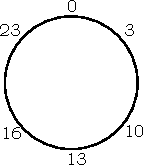
\includegraphics{images/illustrations/modular.pdf}
\end{center}

To reduce a given number using modulo 26 we can use the following function:

\[
 f(x) = x - \left\lfloor{\frac{x}{26}}\right\rfloor \times 26
\]

This says that to obtain the value of a number $x$ using modulo 26 we first divide $x$ by 26 and round down, which gives us the number of times we went around the circle. We then multiply this result by 26 again and subtract this from $x$. The final result is the remainder left over and will always be a value between 0 and 25.

As an example, the number 28 in modulo 26 is equal to 2:
\[
	f(28) = 28 - \left\lfloor{\frac{28}{26}}\right\rfloor \times 26 = 28 - 1 \times 26 = 2
\]

The program at the end of this chapter makes use of this formula by defining a corresponding function at line 30:

\begin{screenoutput}
DEF FN F(X)=X-INT(X/26)*26
\end{screenoutput}

{\bf ROT13:} When we encrypt each plaintext letter we move forward 13 places. So the plaintext letter A becomes the ciphertext letter N, B becomes O, with latter letters "wrapping around" back to the beginning of the alphabet. Thus, the plaintext letter Z becomes the ciphertext letter M. This covers encryption. To decrypt each ciphertext letter we simply repeat the process by moving forward 13 places again, which brings us full circle, back to where we started. Thus, a ciphertext letter N becomes the plaintext letter A.

We can see this visually as a mapping in the form of a table:

\Large
\begin{center}
  \begin{tabular}{|c|c|c|c|c|c|c|c|c|c|c|c|c|c|}
  \hline
    English Plaintext & A & B & C & D & E & F & G & H & I & J & K & L & M \\ \hline
	ROT13 Ciphertext & N & O & P & Q & R & S & T & U & V & W & X & Y & Z \\ \hline
  \end{tabular}
\end{center}

\begin{center}
  \begin{tabular}{|c|c|c|c|c|c|c|c|c|c|c|c|c|c|}
  \hline
    English Plaintext & N & O & P & Q & R & S & T & U & V & W & X & Y & Z \\ \hline
	ROT13 Ciphertext & A & B & C & D & E & F & G & H & I & J & K & L & M \\ \hline
  \end{tabular}
\end{center}

\normalsize

To encrypt using ROT13, find the plaintext letter in the top row and move down to the bottom row to find the corresponding ciphertext letter. To decrypt using ROT13, find the ciphertext letter in the bottom row and move up to the top row to find the corresponding plaintext letter.

If we consider the ROT13 cipher from a mathematical standpoint, we can see that to both encrypt and decrypt we simply add 13 to the numerical value of a plaintext or ciphertext letter and reduce it using modulo 26. This gives us a new number between 0 and 25 which corresponds to the encrypted or decrypted letter. Function $E_{ROT13}$ is the encryption function. It accepts the value of a plaintext letter $x$ as an argument and returns the value of the ciphertext letter as a result. Function $D_{ROT13}$ is the decryption function. It accepts the value of a ciphertext letter $x$ as an argument and returns the value of the plaintext letter as a result.

\[
  E_{ROT13}(x) = (x + 13) \bmod 26
\]

\[
  D_{ROT13}(x) = (x + 13) \bmod 26
\]

Notice that the definitions of both the encryption and decryption functions are, in this case, exactly the same.

{\bf Atbash:} Atbash is an ancient technique used to encrypt the 22-letter Hebrew alphabet, but we can apply the same logic to encrypt the 26-letter English alphabet. To encrypt a letter using Atbash we need to consider the English alphabet written backwards. So encrypting the plaintext letter A becomes the ciphertext letter Z, B becomes Y, C becomes X and so on. Decrypting the ciphertext works the same way: the ciphertext letter A becomes the plaintext letter Z, B becomes Y, C becomes X and so on.

We can see this visually as a mapping in the form of a table:

\Large
\begin{center}
  \begin{tabular}{|c|c|c|c|c|c|c|c|c|c|c|c|c|c|}
  \hline
    English Plaintext & A & B & C & D & E & F & G & H & I & J & K & L & M \\ \hline
	Atbash Ciphertext & Z & Y & X & W & V & U & T & S & R & Q & P & O & N \\ \hline
  \end{tabular}
\end{center}

\begin{center}
  \begin{tabular}{|c|c|c|c|c|c|c|c|c|c|c|c|c|c|}
  \hline
    English Plaintext & N & O & P & Q & R & S & T & U & V & W & X & Y & Z \\ \hline
    Atbash Ciphertext & M & L & K & J & I & H & G & F & E & D & C & B & A \\ \hline
  \end{tabular}
\end{center}

\normalsize

To encrypt using Atbash, find the plaintext letter in the top row and move down to the bottom row to find the corresponding ciphertext letter. To decrypt using Atbash, find the ciphertext letter in the bottom row and move up to the top row to find the corresponding plaintext letter.

If we consider the Atbash cipher from a mathematical standpoint, we can see that to encrypt and decrypt, we need to multiply by 25 and then add 25 to the numerical value of the plaintext or ciphertext and reduce it using modulo 26. This gives us a new number between 0 and 25 which corresponds to the encrypted or decrypted letter. Function $E_{Atbash}$ is the encryption function. It accepts the value of a plaintext letter $x$ as an argument and returns the value of the ciphertext letter as a result. Function $D_{Atbash}$ is the decryption function. It accepts the value of a ciphertext letter $x$ as an argument and returns the value of the plaintext letter as a result.

\[
  E_{Atbash}(x) = (25 \times x + 25) \bmod 26
\]

\[
  D_{Atbash}(x) = (25 \times x + 25) \bmod 26
\]

Notice that the definitions of both the encryption and decryption functions are, in this case, exactly the same.

{\bf Caesar:} The Caesar cipher is also an ancient technique used encrypt and decrypt messages. To encrypt a letter using the Caesar cipher we move three positions forward. So encrypting the plaintext letter A becomes the ciphertext letter D, B becomes E, C becomes F and so on. Decrypting the ciphertext works the opposite way. Instead of moving forward, we move three positions backward. The ciphertext letter A becomes the plaintext letter X, B becomes Y, C becomes Z and so on.

We can see this visually as a mapping in the form of a table:

\Large
\begin{center}
  \begin{tabular}{|c|c|c|c|c|c|c|c|c|c|c|c|c|c|}
  \hline
    English Plaintext & A & B & C & D & E & F & G & H & I & J & K & L & M \\ \hline
	Caesar Ciphertext & D & E & F & G & H & I & J & K & L & M & N & O & P \\ \hline
  \end{tabular}
\end{center}

\begin{center}
  \begin{tabular}{|c|c|c|c|c|c|c|c|c|c|c|c|c|c|}
  \hline
    English Plaintext & N & O & P & Q & R & S & T & U & V & W & X & Y & Z \\ \hline
    Caesar Ciphertext & Q & R & S & T & U & V & W & X & Y & Z & A & B & C \\ \hline
  \end{tabular}
\end{center}

\normalsize

To encrypt using the Caesar cipher, find the plaintext letter in the top row and move down to the bottom row to find the corresponding ciphertext letter. To decrypt using the Caesar cipher, find the ciphertext letter in the bottom row and move up to the top row to find the corresponding plaintext letter.

If we consider the Casear cipher from a mathematical standpoint, we can see that to encrypt, we need to add 3 to the numerical value of the plaintext and reduce it using modulo 26. This gives us a new number between 0 and 25 which corresponds to the encrypted letter. To decrypt, we need to subtract 3 from the numerical value of the ciphertext and reduce it modulo 26. This gives us a new number between 0 and 25 which corresponds to the decrypted letter.

Function $E_{Caesar}$ is the encryption function. It accepts the value of a plaintext letter $x$ as an argument and returns the value of the ciphertext letter as a result. Function $D_{Caesar}$ is the decryption function. It accepts the value of a ciphertext letter $x$ as an argument and returns the value of the plaintext letter as a result.

\[
  E_{Caesar}(x) = (x + 3) \bmod 26
\]

\[
  D_{Caesar}(x) = (x - 3) \bmod 26
\]

Notice that the definitions of both the encryption and decryption functions are, in this case, different.

We can generalise all three of the above methods by stating that they use the following encryption and decryption functions:

\[
 E(x) = (A_{1}x + B_{1}) \bmod 26
\]

\[
 D(x) = (A_{2}x + B_{2}) \bmod 26
\]

Here, $A_{1}$, $A_{2}$, $B_{1}$ and $B_{2}$ are constants and put together they comprise the {\it encryption key} for an affine cipher.

Running the following program displays a text menu. The user can choose to encrypt or decrypt a string, or quit the program. You can practice typing in a plaintext phrase to encrypt and then decrypt the ciphertext phrase to retrieve the orginal plaintext.

A good sample text string for testing a cipher is:

\texttt{\bf THE QUICK BROWN FOX JUMPS OVER THE LAZY DOG}

This text string, which is 43 characters long, contains 8 spaces and 35 alphabetic characters. Every character of the alphabet occurs at least once in this string, so encrypting and decrypting with it checks that every letter is transformed as expected.

Encrypting the above text string using the ROT13 cipher yields:

\texttt{\bf GUR DHVPX OEBJA SBK WHZCF BIRE GUR YNML QBT}

Encrypting the above text string using the Atbash cipher yields:

\texttt{\bf GSV JFRXP YILDM ULC QFNKH LEVI GSV OZAB WLT}

Encrypting the above text string using the Caesar cipher yields:

\texttt{\bf WKH TXLFN EURZQ IRA MXPSV RYHU WKH ODCB GRJ}

\begin{screenoutput}
10 REM *** CRYPTOGRAPHY ***
20 POKE 0,65: PRINT CHR$(142): PRINT CHR$(147)
30 DEF FN F(X)=X-INT(X/26)*26
40 C$="": P$=""
50 PRINT "SELECT AN OPTION (E, D OR Q):": PRINT
60 PRINT "{SPACE*3}[E] ENCRYPT PLAINTEXT": PRINT
70 PRINT "{SPACE*3}[D] DECRYPT CIPHERTEXT": PRINT
80 PRINT "{SPACE*3}[Q] QUIT": PRINT
90 GET S$
100 IF (S$="Q") THEN END
110 IF (S$="E") THEN GOSUB 150: GOTO 40
120 IF (S$="D") THEN GOSUB 270: GOTO 40
130 GOTO 90
140 REM ENCRYPT
150 INPUT "ENTER PLAINTEXT MESSAGE TO ENCRYPT: ", P$
160 IF P$="" THEN GOTO 150
170 M$=P$: GOSUB 390
180 IF (V=0) THEN GOSUB 460: GOTO 150
190 A=1:B=3
200 FOR I=1 TO LEN(P$)
210 :   L$ = MID$(P$,I,1)
220 :   IF (L$=" ") THEN C$=C$+" ": ELSE C$=C$+CHR$(65+(FN F(A*(ASC(L$)-65)+B)))
230 NEXT I
240 PRINT: PRINT "{REVERSE ON}ENCRYPTED CIPHERTEXT:{REVERSE OFF}", C$: PRINT
250 RETURN
260 REM DECRYPT
270 INPUT "ENTER CIPHERTEXT MESSAGE TO DECRYPT: ", C$
280 IF C$="" THEN GOTO 270
290 M$=C$: GOSUB 390
300 IF (V=0) THEN GOSUB 460: GOTO 270
310 A=1: B=-3
320 FOR I=1 TO LEN(C$)
330 :   L$ = MID$(C$,I,1)
340 :   IF (L$=" ") THEN P$=P$+" ": ELSE P$=P$+CHR$(65+(FN F(A*(ASC(L$)-65)+B)))
350 NEXT I
360 PRINT: PRINT "{REVERSE ON}DECRYPTED PLAINTEXT:{REVERSE OFF}", P$: PRINT
370 RETURN
380 REM VALIDATE
390 V = 1
400 FOR I=1 TO LEN(M$)
410 :   L$ = MID$(M$,I,1)
420 :   IF NOT (((L$ >= "A") AND (L$ <= "Z")) OR (L$=" ")) THEN V = 0
430 NEXT I
440 RETURN
450 REM ERROR MESSAGE
460 PRINT: PRINT "USE LETTERS AND SPACES ONLY": PRINT
470 RETURN
\end{screenoutput}

If you wish to use the ROT13 cipher ensure that the following lines are changed:
\begin{screenoutput}
190 A=1: B=13
310 A=1: B=13
\end{screenoutput}

If you wish to use the Atbash cipher ensure that the following lines are changed:
\begin{screenoutput}
190 A=25: B=25
310 A=25: B=25
\end{screenoutput}

If you wish to use the Caesar cipher ensure that the following lines are changed:
\begin{screenoutput}
190 A=1: B=3
310 A=1: B=-3
\end{screenoutput}

The program listing, as written, uses the Caesar cipher by default.

\input{morebasic}
\input{datainbasic}
\chapter {C64, C65 and MEGA65 Modes}
\label{cha:modes}

The MEGA65, like the C65 and the C128, has multiple operating modes,
however there are important differences between the MEGA65 and both
of these earlier computers.  For people familiar with the C128,
the most important difference is that all of the MEGA65's new features
can be accessed from every mode, and you can even switch back and forth
between the different modes, or create hybrid modes that combine different
features from the different modes -- all you need is the MAP and KEY.

This chapter explains the different modes, the MAP instruction and
the KEY register, that allows you to change the mode of operation of the computer,
as well instructions on how to use BASIC commands to completely switch
from one mode to another.

\phantomsection
\section{Switching Modes from BASIC}

At the time of writing, there is no MEGA65 Mode BASIC. The MEGA65 is used either
in C64 mode (running BASIC 2), or C65 mode (running BASIC 65).  However, various MEGA65
features can be accessed from both C64 and C65 mode.  All MEGA65 features are available
to programs written in assembly language / machine code.  The information required
to write such programs can be found in the various appendices.

\subsection{From C65 to C64 Mode}

To switch from C65 to C64 Mode, use the familiar GO 64 command, which is identical to switching to C64
mode on a C128:

\begin{tcolorbox}[colback=black,coltext=white]
\verbatimfont{\codefont}
\begin{verbatim}
GO 64
ARE YOU SURE? Y
\end{verbatim}
\end{tcolorbox}

Note that, just like on the C128, any programs in memory will be lost in the process of switching modes.

Alternatively, you can hold down the MEGA key when pressing the reset button or turning the computer on. Again,
this is the same as on the C128.

\subsection{From C64 to C65 Mode}

To switch from C64 to C65 mode, use the following command. {\bf Note that this command does not ask you for
confirmation}!

\begin{tcolorbox}[colback=black,coltext=white]
\verbatimfont{\codefont}
\begin{verbatim}
SYS 58552
\end{verbatim}
\end{tcolorbox}

Alternatively, you can switch back to C65 mode by pressing the reset
button on the left side of the computer, or simply by turning the
computer off and on again.

Another option is to long-press the \widekey{RESTORE} key, and then press \megakey {F5}
from the freeze menu.  This simulates pressing the reset button.

Note that, just like on the C128, any programs in memory will be
lost in the process of switching modes.

\subsection{Entering Machine Code Monitor Mode}

The machine code monitor can be entered by typing either the MONITOR
command from BASIC 65 in C65 mode, or by holding the RUN/STOP key
down, and then pressing the reset button on the left side of the
computer.

\phantomsection
\section{The KEY Register}

The MEGA65 has a VIC-IV video controller chip instead of the C64's VIC-II or
the C65's VIC-III.  Just as the VIC-III has extra registers compared to the
VIC-II, the VIC-IV has even more registers.  If these were visible all the time,
software that was made for the C64 and it's VIC-II may accidentally use the
new registers, resulting in unexpected behaviour.  Therefore, the
creators of the C65 created a way to hide the extra VIC-III registers from old
C64 programs. This is called the KEY register. For more information
about which registers are disabled, and enabled in each of the
VIC-II, VIC-III and VIC-IV IO modes, refer to
\ifdefined\printmanual
 the {\bf MEGA65 Book}.
\else
 \bookvref{sec:iopersonalities}.
\fi

% iopersonalities results in ?? (??) when building on my machine

The KEY register at address 53295 (hex \$D02F) is an unused register of the VIC-II, which you can POKE to and
PEEK from, like other registers.  But the KEY register has a special function: If
you write two certain values to it in quick succession, you can tell the VIC-IV
to stop hiding the VIC-III or VIC-IV registers from the rest of the computer.

\subsection{Exposing Extra C65 Registers}

For example, to enable the VIC-III's new registers when in C64 mode, you must POKE the values 165 and 150
into the KEY register. The easiest way to do this is to turn your MEGA65 off and on again, and type GO 64
and answer YES to enter C64 mode.

If you do this C65 mode, the computer may not function correctly.

Once you are in C64 mode, try typing the following commands:

\begin{tcolorbox}[colback=black,coltext=white]
\verbatimfont{\codefont}
\begin{verbatim}
POKE 53295,165: POKE 53295,150
\end{verbatim}
\end{tcolorbox}

When you enter these commands, the computer returns a \screentextwide{READY.} prompt, and seemingly nothing else has
happened.  This is expected, because the computer has only enabled the VIC-III's new registers (and some other
C65 mode features). The C64 BASIC and KERNAL will still function as normal, and it may appear
that nothing has changed... But things \textit{have} changed.

As an example, you can do something that the C64 and its VIC-II can't do: smoothly change one colour to another.
The VIC-III has registers that allow you to change the red, green and blue components of the colours. Now that the VIC-III
registers are enabled, it's possible to change the colour of the background progressively from blue to purple, by increasing
the red component of the colour that is normally blue on the C64.  The red component value registers are at
53504 -- 53759 (hex \$D100 -- \$D1FF). Blue is colour 6, so a change to register 53504 + 6 = 53510 (hex \$D106) is required.
An example BASIC listing below includes a FOR loop to change the colour:

\begin{tcolorbox}[colback=black,coltext=white]
\verbatimfont{\codefont}
\begin{verbatim}
FOR I = 0 TO 15 STEP 0.2 : POKE 53510,I : NEXT
\end{verbatim}
\end{tcolorbox}

Once the program has been entered, type RUN on a new line. This will make the background of the screen fade from
blue to purple.  If you would like to make the effect progress faster, increase the 0.2 to a larger number, such as 0.5, or to
make it slower, change it to a smaller number, such as 0.02. You can also change the red component by adding a
different number to 53504, the green component at 53760 -- 54015 (hex \$D200 -- \$D2FF), or the
blue component at 54016 -- 54271 (hex \$D300 -- \$D3FF).  For example, to have
the border and text (since they are both normally ``light blue'') fade from blue to green, you can try:

\begin{tcolorbox}[colback=black,coltext=white]
\verbatimfont{\codefont}
\begin{verbatim}
POKE 53518,0 : FOR I = 0 TO 15 STEP 0.1 : POKE 53774,I : POKE 54030,15-I : NEXT
\end{verbatim}
\end{tcolorbox}

\subsection{Disabling the C65/MEGA65 Extra Registers}

You can also disable the VIC-III registers again by POKEing any number you like into the KEY register, e.g.:

\begin{tcolorbox}[colback=black,coltext=white]
\verbatimfont{\codefont}
\begin{verbatim}
POKE 53295,0
\end{verbatim}
\end{tcolorbox}

If you RUN the examples above again, the colours won't change because
the registers are disabled. Instead, writing to those addresses changes some of the VIC-II's registers,
as on a C64 they appear several times over.  Fortunately for the above example, the registers used have no obvious
side-effects. This is because the modified registers in the examples above on a standard VIC-II are used to change the
sprite positions. As there are no sprites on the screen, you won't see any problems.

\subsection{Enabling MEGA65 Extra Registers}

The MEGA65 has \textit{even more} registers than the C65.  To enable these in C64 mode, it's required to POKE another
two values into the KEY register:

\begin{tcolorbox}[colback=black,coltext=white]
\verbatimfont{\codefont}
\begin{verbatim}
POKE 53295,71: POKE 53295,83
\end{verbatim}
\end{tcolorbox}

Again, you won't see any immediate difference, just like when enabling the C65 / VIC-III registers.  However, now the computer
can access not only the C64 / VIC-II, and C65 / VIC-III registers, but also the MEGA65 / VIC-IV registers.  If you like,
you can try the examples from earlier in this chapter, to see that the C65 / VIC-III registers are accessible again.
But now you can also do MEGA65 specific things. For example, if you wanted to move the start of the top border higher
on the screen, you can try something like:

\begin{tcolorbox}[colback=black,coltext=white]
\verbatimfont{\codefont}
\begin{verbatim}
POKE 53320,60
\end{verbatim}
\end{tcolorbox}

Or you can have some fun, and animate the screen borders, by having them move closer and further apart:

\begin{tcolorbox}[colback=black,coltext=white]
\verbatimfont{\codefont}
\begin{verbatim}
FOR I = 255 TO 0 STEP -1 : POKE 53320,I : POKE 53322, 255 - I : NEXT
\end{verbatim}
\end{tcolorbox}

The above example has the loop count backwards (from 255 to 0), so that your don't end up with only a
tiny sliver of the text visible. You can make it go forwards if you like. If you do get stuck with a sliver
of the screen, you can press RUN/STOP and RESTORE. You might be wondering: Why does RUN/STOP
and RESTORE work when these are MEGA65 / VIC-IV registers that the C64-mode BASIC and KERNAL
don't know about?  The reason is the VIC-IV has a feature called ``hot registers'',
where certain C64 and C65 registers cause some MEGA65 registers to be reset to the C64 or
C65 mode defaults. In this particular case, it is the KERNAL resetting the VIC-II screen using
53265 (hex \$D011), which adjusts the vertical border size in C64/C65 mode, and is thus a ``hot register''
for the MEGA65's vertical border position registers.

See if you can instead make the screen shake around by changing the TEXTXPOS and TEXTYPOS registers of
the VIC-IV.  You can find out the POKE codes for those, and lots of other interesting new registers
by looking through
\ifdefined\printmanual
 the {\bf MEGA65 Book}.
\else
 \bookvref{cha:viciv}.
\fi


\subsection{Traps to look out for}

In both C64 and C65 mode, the DOS for the internal 3.5'' disk drive (including when you use D81 disk images from
an SD card) resets the KEY register to C64 / VIC-II mode whenever it is accessed. This means if you perform actions,
such as check the drive status, or LOAD or SAVE a file, the KEY register will be reset, and only the C64 / VIC-II registers
will be enabled. You can of course enable the C65 or MEGA65 registers by POKEing the correct values
to the KEY register again.

\phantomsection
\section{Accessing Memory from BASIC 65}

The C65's BASIC 65 contains powerful memory banking and Direct Memory Access (DMA) commands that can be used to read,
fill, copy, and write areas of memory beyond the C65's 128KB of RAM.  The MEGA65 has 384KB of main memory. Of this,
the first 128KB (BANK 0 and BANK 1) acts as the C65's normal 128KB RAM. The second 128KB (BANK 2 and BANK 3) is normally
write-protected, and is used to hold the C65's ROM image.  The last 128KB (BANK 4 and BANK 5) is however completely free.

Using the BANK, PEEK and POKE commands, this region of memory can be easily accessed, for example:

\begin{tcolorbox}[colback=black,coltext=white]
\verbatimfont{\codefont}
\begin{verbatim}
BANK 4: POKE0,123: REM PUT 123 IN LOCATION $40000
BANK 4: PRINT PEEK(0): REM SHOW CONTENTS OF LOCATION $40000
\end{verbatim}
\end{tcolorbox}

Or, by using the DMA command, you can copy the current contents of the screen and colour RAM into BANK 4 with:

\begin{tcolorbox}[colback=black,coltext=white]
\verbatimfont{\codefont}
\begin{verbatim}
DMA 0, 2000, 2048, 0, 0, 4 : REM SCREEN TEXT TO BANK 4
DMA 0, 2000, DEC("F800"), 1, 2000, 4 : REM COPY COLOUR RAM TO BANK 4
\end{verbatim}
\end{tcolorbox}

You can then put something else on the screen, and then copy it back with:

\begin{tcolorbox}[colback=black,coltext=white]
\verbatimfont{\codefont}
\begin{verbatim}
DMA 0, 2000, 0, 4, 2048, 0, : REM SCREEN TEXT FROM BANK 4
DMA 0, 2000, 2000, 4, DEC("F800"), 1 : REM COPY COLOUR RAM FROM BANK 4
\end{verbatim}
\end{tcolorbox}

Note that there is currently no way to tell BASIC 65 to put graphics screen, variables,
arrays or program text in these extra banks of RAM.

\phantomsection
\section{The MAP Instruction}

The above methods can be used from BASIC. In contrast, the MAP instruction is an assembly
language instruction that can be used to rearrange the memory that the MEGA65 uses.
It is used by the C65 ROM and BASIC 65 to manage what memory it can use at any particular
point in time.  For further explanation of the MAP instruction,
refer to the relevant section of
\ifdefined\printmanual
 the {\bf MEGA65 Book}.
\else
 \bookvref{sec:map-instruction}.
\fi





\part{SOUND AND GRAPHICS}

%\usepackage{colortbl}
%\usepackage{adjustbox}


\newcommand{\blkb}{\cellcolor[rgb]{0,0,0}\textcolor{white} 0 }
\newcommand{\bwn}{\cellcolor[rgb]{.26,.22,0}\textcolor{white} 9 }
\newcommand{\ora}{\cellcolor[rgb]{.44,.31,.15} 8 }
\newcommand{\red}{\cellcolor[rgb]{.6,.4,.35} A }
\newcommand{\lgr}{\cellcolor[rgb]{.58,.58,.58} F }
\newcommand{\yel}{\cellcolor[rgb]{.72,.78,.44} 7 }

\newcommand{\redb}{\cellcolor[rgb]{.6,.4,.35} 1 }

\chapter{Graphics}
\label{cha:graphics}

Let's have some fun with graphics!
In this part of the book, we want to examine the MEGA65's graphics modes by walking through example code in machine language to get to know the various options of the MEGA65 in the area of graphics. First of all, it is important to know that the MEGA65 supports three different basic graphics modes:

\begin{itemize}
	\item Bitmap graphics
	\item Graphics based on character sets
	\item Bitplanes
\end{itemize}


\section*{Bitmap Graphics}

In bitmap graphics every pixel of a graphic is stored separately. The way the pixels are hold in memory varies from system to system and in most cases depends on the performance of the hardware. If memory would be unlimited, the easiest way to remember a pixel is to save its RGB-values in three separate bytes. Example: 0xFFFFFF for white would result in three values to be stored: \$FF, \$FF and \$FF. To be honest, this is too simple and not really efficient. Let’s think about another way. Why not defining a color table (or color palette) and store the RGB values once and finally only reference the color by its index in the table? This will save us a lot of memory! Let's imagine we would create a colorful 8x8 bitmap to represent an "A" on the screen. Colourful means, we want it in some brownish colors. The color table for it may look like this:

%\setlength\minrowclearance{4pt}
\begin{center}
\begin{tabular}{|m{22pt}|m{60pt}|}
\hline
	Index & Color \\
\hline
	\blkb & Black \\
	\bwn & Brown \\
	\ora & Orange \\
	\red & Light Red \\
	\lgr & Light Grey \\
	\yel & Yellow \\
\hline
\end{tabular}
\end{center}

The color values, by the way, are exact the same as the color values from the standard C64 color palette. Next we design the "A". Each pixel references a value from the color table above.


%\setlength\minrowclearance{4pt}
\begin{center}
\begin{tabular}{|m{4pt}|m{4pt}m{4pt}m{4pt}m{4pt}m{4pt}m{4pt}m{4pt}m{4pt}|}
\hline
	& 7 & 6 & 5 & 4 & 3 & 2 & 1 & 0 \\
\hline
	0 & \blkb & \blkb & \blkb & \blkb & \blkb & \blkb & \blkb & \blkb \\
	1 & \red & \lgr & \yel & \lgr & \red & \ora & \blkb & \blkb \\
	2 & \lgr & \lgr & \blkb & \blkb & \ora & \red & \blkb & \blkb \\
	3 & \yel & \yel & \blkb & \blkb & \ora & \red & \blkb & \blkb \\
	4 & \yel & \lgr & \lgr & \red & \red & \red & \blkb & \blkb \\
	5 & \lgr & \red & \blkb & \blkb & \ora & \red & \blkb & \blkb \\
	6 & \red & \red & \blkb & \blkb & \red & \red & \blkb & \blkb \\
	7 & \ora & \bwn & \blkb & \blkb & \ora & \red & \blkb & \blkb \\
\hline
\end{tabular}
\end{center}

But how much memory does this little graphic use?

If we create an one-dimensional array, we will get an array with 64 elements, because our graphic consists of 8x8 pixels = 64 color values that have to be saved. If we transfer that to the memory of the MEGA65, it means that we have 64 bytes to store in memory. However, full-screen graphics are made up of far more pixels. On the C64 and of course also on the MEGA65, 320x200 pixels are required to generate a graphic that fills the entire screen. If we transfer this to our array, we would have a total of 64,000 entries. Converted to the memory of the MEGA65, that is 64,000 bytes or nearly 64 kilobytes of data! If we now also consider that the good old C64 only had 64K of RAM available, we recognize the Drama! That's just too much data! We need strategies to reduce our bitmap data. On the C64 we had to two types of bitmap graphics and both come with its own concepts to use as less memory as possible.

\begin{itemize}
	\item Hires
	\item Multicolor (MCM)
\end{itemize}


\subsection*{Hires}

First, a bitmap is divided into blocks of 8x8 pixels each. In order to achieve the full resolution of 320x200 pixels, 40 of such blocks next to each other builds up a line. If we now build up 25 lines, we arrive at a graphic that fills the complete screen.

\begin{adjustbox}{width=\textwidth,center}
\begin{center}
\begin{footnotesize}
\begin{tabular}[h]{|C{10pt}|C{5pt}|C{5pt}|C{5pt}|C{5pt}|C{5pt}|C{5pt}|C{5pt}|C{5pt}|C{5pt}|C{5pt}|C{5pt}|C{5pt}|C{5pt}|C{5pt}|C{5pt}|C{5pt}|C{5pt}|C{5pt}|C{5pt}|C{5pt}|C{5pt}|C{5pt}|C{5pt}|C{5pt}|C{5pt}|C{5pt}|C{5pt}|C{5pt}|C{5pt}|C{5pt}|C{5pt}|C{5pt}|C{5pt}|C{5pt}|C{5pt}|C{5pt}|C{5pt}|C{5pt}|C{5pt}|C{5pt}|}
\hline
  &   &   &  &  &  &   &   &   &   & 1  & 1  & 1  & 1  & 1  & 1  & 1  & 1  & 1  & 1  & 2  & 2  & 2  & 2  & 2  & 2  & 2  & 2  & 2  & 2  & 3  & 3  & 3  & 3  & 3  & 3  & 3  & 3  & 3  & 3  & 4  \\
  & 1 & 2 & 3& 4& 5& 6 & 7 & 8 & 9 &  0 & 1  &  2 &  3 &  4 &  5 &  6 &  7 &  8 &  9 &  0 &  1 &  2 &  3 &  4 &  5 &  6 &  7 &  8 &  9 &  0 &  1 &  2 &  3 &  4 &  5 &  6 &  7 &  8 &  9 &  0 \\
\hline
   1 & & & & & & & & & & & & & & & & & & & & & & & & & & & & & & & & & & & & & & & & \\\hline
   2 & & & & & & & & & & & & & & & & & & & & & & & & & & & & & & & & & & & & & & & & \\\hline
   3 & & & & & & & & & & & & & & & & & & & & & & & & & & & & & & & & & & & & & & & & \\\hline
   4 & & & & & & & & & & & & & & & & & & & & & & & & & & & & & & & & & & & & & & & & \\\hline
   5 & & & & & & & & & & & & & & & & & & & & & & & & & & & & & & & & & & & & & & & & \\\hline
   6 & & & & & & & & & & & & & & & & & & & & & & & & & & & & & & & & & & & & & & & & \\\hline
   7 & & & & & & & & & & & & & & & & & & & & & & & & & & & & & & & & & & & & & & & & \\\hline
   8 & & & & & & & & & & & & & & & & & & & & & & & & & & & & & & & & & & & & & & & & \\\hline
   9 & & & & & & & & & & & & & & & & & & & & & & & & & & & & & & & & & & & & & & & & \\\hline
  10 & & & & & & & & & & & & & & & & & & & & & & & & & & & & & & & & & & & & & & & & \\\hline
  11 & & & & & & & & & & & & & & & & & & & & & & & & & & & & & & & & & & & & & & & & \\\hline
  12 & & & & & & & & & & & & & & & & & & & & & & & & & & & & & & & & & & & & & & & & \\\hline
  13 & & & & & & & & & & & & & & & & & & & & & & & & & & & & & & & & & & & & & & & & \\\hline
  14 & & & & & & & & & & & & & & & & & & & & & & & & & & & & & & & & & & & & & & & & \\\hline
  15 & & & & & & & & & & & & & & & & & & & & & & & & & & & & & & & & & & & & & & & & \\\hline
  16 & & & & & & & & & & & & & & & & & & & & & & & & & & & & & & & & & & & & & & & & \\\hline
  17 & & & & & & & & & & & & & & & & & & & & & & & & & & & & & & & & & & & & & & & & \\\hline
  18 & & & & & & & & & & & & & & & & & & & & & & & & & & & & & & & & & & & & & & & & \\\hline
  19 & & & & & & & & & & & & & & & & & & & & & & & & & & & & & & & & & & & & & & & & \\\hline
  20 & & & & & & & & & & & & & & & & & & & & & & & & & & & & & & & & & & & & & & & & \\\hline
  21 & & & & & & & & & & & & & & & & & & & & & & & & & & & & & & & & & & & & & & & & \\\hline
  22 & & & & & & & & & & & & & & & & & & & & & & & & & & & & & & & & & & & & & & & & \\\hline
  23 & & & & & & & & & & & & & & & & & & & & & & & & & & & & & & & & & & & & & & & & \\\hline
  24 & & & & & & & & & & & & & & & & & & & & & & & & & & & & & & & & & & & & & & & & \\\hline
  25 & & & & & & & & & & & & & & & & & & & & & & & & & & & & & & & & & & & & & & & & \\\hline
\end{tabular}
\end{footnotesize}
\end{center}

\end{adjustbox}

Splitting into blocks makes sense because this gives us the chance to reduce the data drastically. Each line of a 8x8 block are 8 bits, so why not forget the color indexes and just say each pixel set represents a "1" in the line and each pixel not set corresponds to "0".

%\setlength\minrowclearance{4pt}
\begin{center}
\begin{tabular}{|m{4pt}|m{4pt}m{4pt}m{4pt}m{4pt}m{4pt}m{4pt}m{4pt}m{4pt}|m{6pt}R{20pt}m{20pt}{18pt}|}
\hline
	& 7 & 6 & 5& 4& 3&  2& 1& 0 & & & & \\
\hline
0 & \blkb & \blkb  & \blkb  & \blkb  & \blkb  & \blkb  & \blkb & \blkb & = & 0 & \to & \$00 \\
1 & \blkb & \redb & \redb & \redb & \redb & \blkb  & \blkb & \blkb & = & 120 & \to & \$78 \\
2 & \redb & \redb & \blkb  & \blkb  & \redb & \redb & \blkb & \blkb & = & 204 & \to & \$CC \\
3 & \redb & \redb & \blkb  & \blkb  & \redb & \redb & \blkb & \blkb & = & 204 & \to & \$CC \\
4 & \redb & \redb & \redb & \redb & \redb & \redb & \blkb & \blkb & = & 252 & \to & \$FC \\
5 & \redb & \redb & \blkb  & \blkb  & \redb & \redb & \blkb & \blkb & = & 204 & \to & \$CC \\
6 & \redb & \redb & \blkb  & \blkb  & \redb & \redb & \blkb & \blkb & = & 204 & \to & \$CC \\
7 & \redb & \redb & \blkb  & \blkb  & \redb & \redb & \blkb & \blkb & = & 204 & \to & \$CC \\
\hline
\end{tabular}
\end{center}

%\setlength\minrowclearance{0}

As shown above now you can easily convert the bits of each line to its hex value and you finally get 8 bytes of data. This is the central idea in hires graphics and with this concept you save a lot of memory. Here in this example it's 8 Bytes versus 64 Bytes if you have to manage all the color references.
Let's count it up for a full screen picture: We have 40x25 Blocks, that is 1000 blocks in total. Each block is 8 Bytes or 1 Kilobyte, so we'll result in "only" 10K for a full screen picture.\\

This is a brilliant solution, but now have a problem: We lost the colors!\\

If you look at the first figure, it was very colorful. But do we really need so many colors? This is the second important concept in hires bitmap graphics: Less colors means less memory. In fact hires mode limits you to \textbf{two colors} per 8x8 pixel block. This information is stored in the Screen-RAM, not in the Color-RAM as one might assume. And again the idea why is really clever: In Screen-RAM you can hold values between \$00 and \$FF whereas in the Color-RAM it makes only sense to store values between \$0 and \$0F to reference one specific color from the C64 color palette which consists of 16 colors (\$0-\$F). On the MEGA65 you can have even more colors and you are able to tweak the default colors, but this will be explained later.\\

Back to the Screen-RAM. Here you store \textbf{two colors} for each 8x8 block. If you split the byte into its Hi-Byte and Low-Byte you have the chance to put a background and a foreground color into it! The value \$0a for example can be seen as \$0 and \$a. This way we'll get a black background and light red for the pixels in the block. In the end this means, a fullscreen hires bitmap will consume not 10 but 20 Kilobytes. 10K for the raw bitmap data as mentioned earlier and another 10K for the colors inside the Screen-RAM.\\


\subsection*{Programming simple Hires Bitmaps}

Let's code!


\input{sprites}
\input{sound}

\part{HARDWARE}

\chapter{Using Nexys4 boards as a MEGA65}

\section{Building your own MEGA65 Compatible Computer}

You can build your own MEGA65-compatible computer by using either a Nexys4DDR (aka. Nexys A7) or the older Nexys4 (Non-DDR) FPGA development boards.
This appendix describes the process to set up a Nexys4DDR (Nexys A7) board for this purpose (which is the newer, preferred board).
The older non-DDR Nexys4 board is also supported, and the instructions are the same, except that
you must use a bitstream designed for that board.
Using a Nexys4DDR bitstream on a non-DDR Nexys4 board, or vice versa, may cause irreparable damage to your board, so make sure
you have the correct bitstream to suit your board.


DISCLAIMER: M.E.G.A cannot take any responsibility for any damage that may occur to your Nexys4DDR/NexysA7/Nexys4 boards.

\newpage

\section{Working Nexys4 Boards}

There are currently 3 Nexys FPGA boards which can be setup as a MEGA65:

\begin{minipage}{\linewidth}
  \subsection{The Nexys4 board}

  No longer manufactured but still available for sale on some websites with old stock.

  \begin{center}
    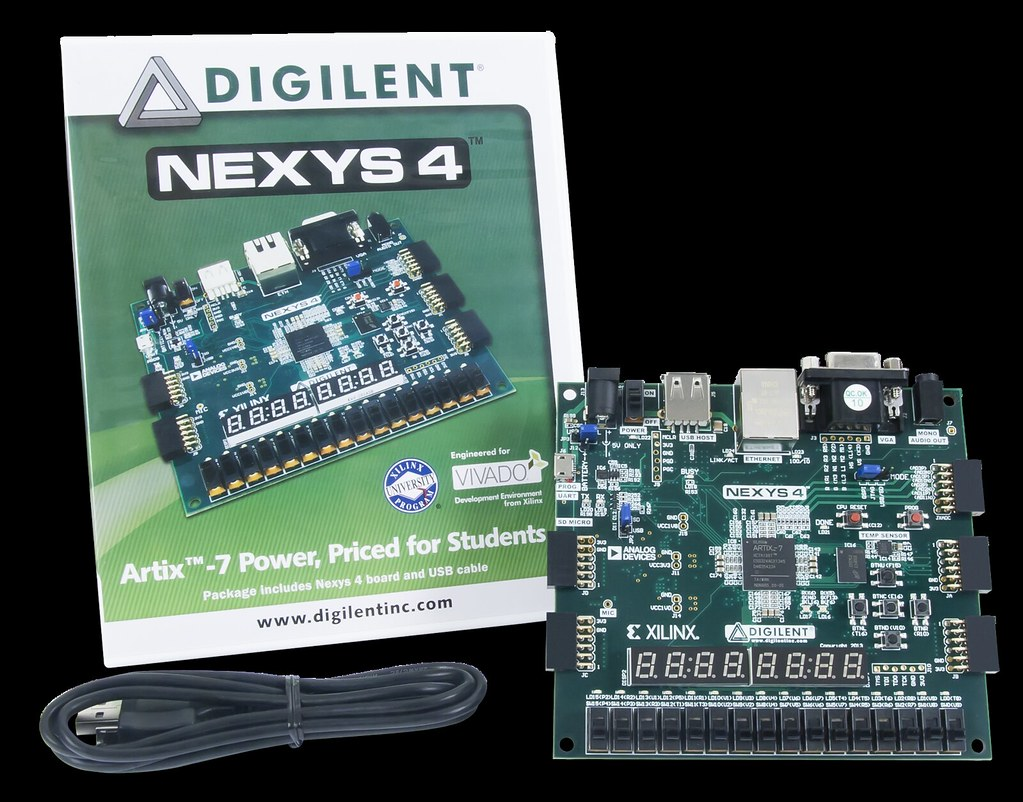
\includegraphics[width=0.4\linewidth]{images/img001_nexys4_board.jpg}
  \end{center}

  Documentation:

  \begin{itemize}
    \item \url{https://reference.digilentinc.com/reference/programmable-logic/nexys-4/reference-manual}
    \item \url{https://reference.digilentinc.com/\_media/reference/programmable-logic/nexys-4/nexys4\_rm.pdf}
  \end{itemize}
\end{minipage}

\begin{minipage}{\linewidth}
  \subsection{The Nexys4DDR board}

  No longer manufactured but still available for sale on some websites with old stock.

  \begin{center}
    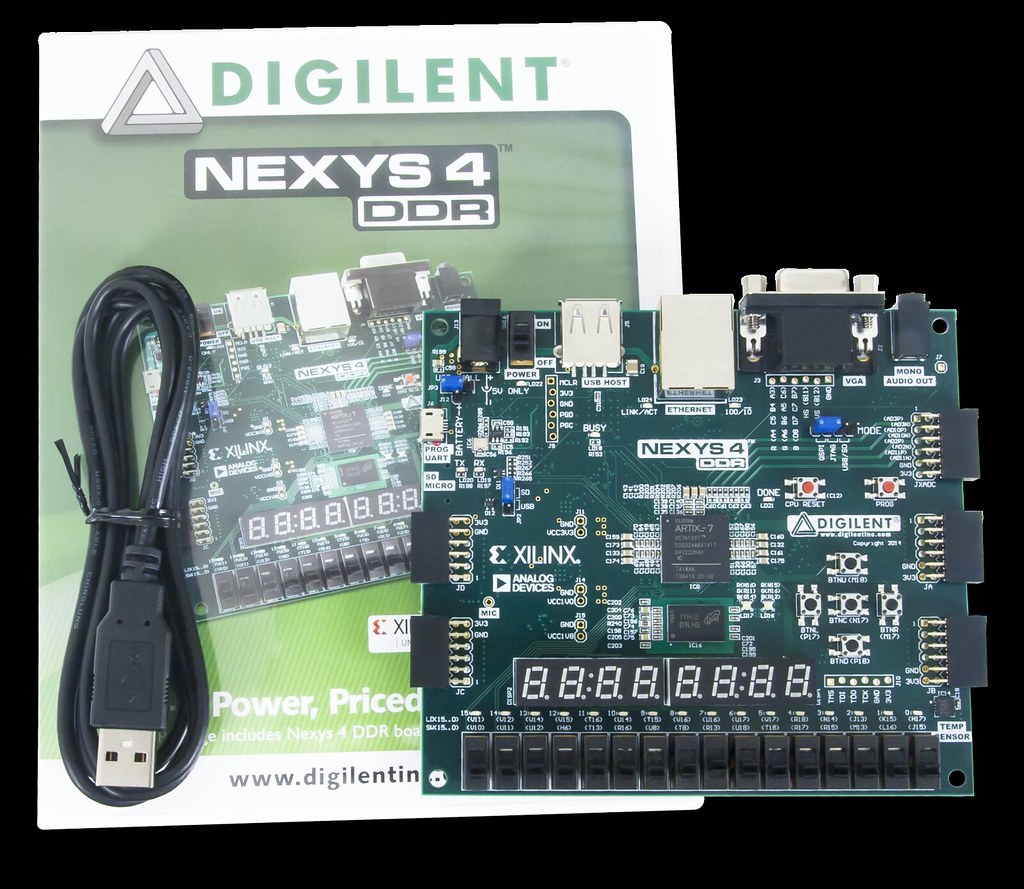
\includegraphics[width=0.4\linewidth]{images/img002_nexys4_ddr_board.jpg}
  \end{center}

  Documentation:

  \begin{itemize}
    \item \url{https://reference.digilentinc.com/reference/programmable-logic/nexys-4-ddr/reference-manual}
    \item \url{https://reference.digilentinc.com/\_media/reference/programmable-logic/nexys-4-ddr/nexys4ddr\_rm.pdf}
  \end{itemize}
\end{minipage}

\begin{minipage}{\linewidth}
  \subsection{The Nexys A7}

  This is the re-branded version of the above Nexys4 DDR board:

  \begin{center}
    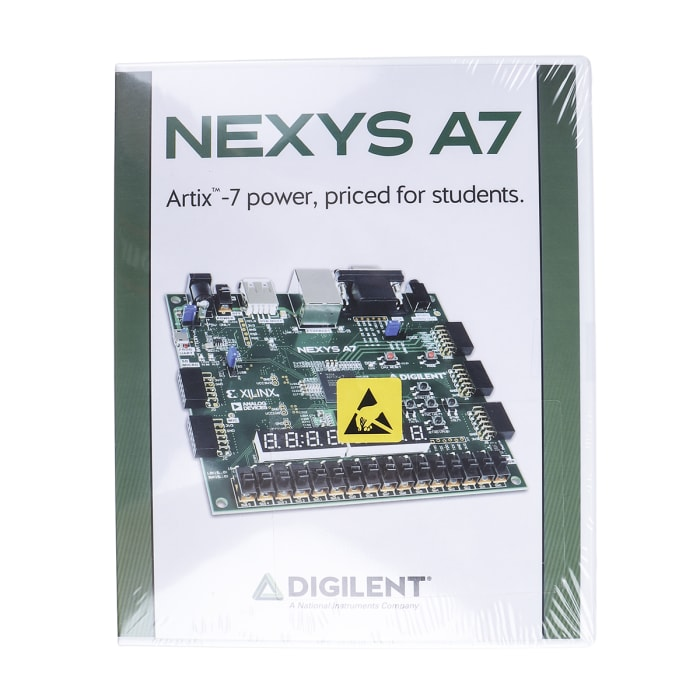
\includegraphics[width=0.4\linewidth]{images/img003_nexysA7_board.jpg}
  \end{center}

  Documentation:

  \begin{itemize}
    \item \url{https://reference.digilentinc.com/reference/programmable-logic/nexys-a7/reference-manual}
    \item \url{https://reference.digilentinc.com/\_media/reference/programmable-logic/nexys-a7/nexys-a7\_rm.pdf}
  \end{itemize}
\end{minipage}

\newpage

\section{Power, Jumpers, Switches and Buttons}

This top-down picture highlights the key jumper positions of interest on the Nexys4 board:

  \begin{center}
    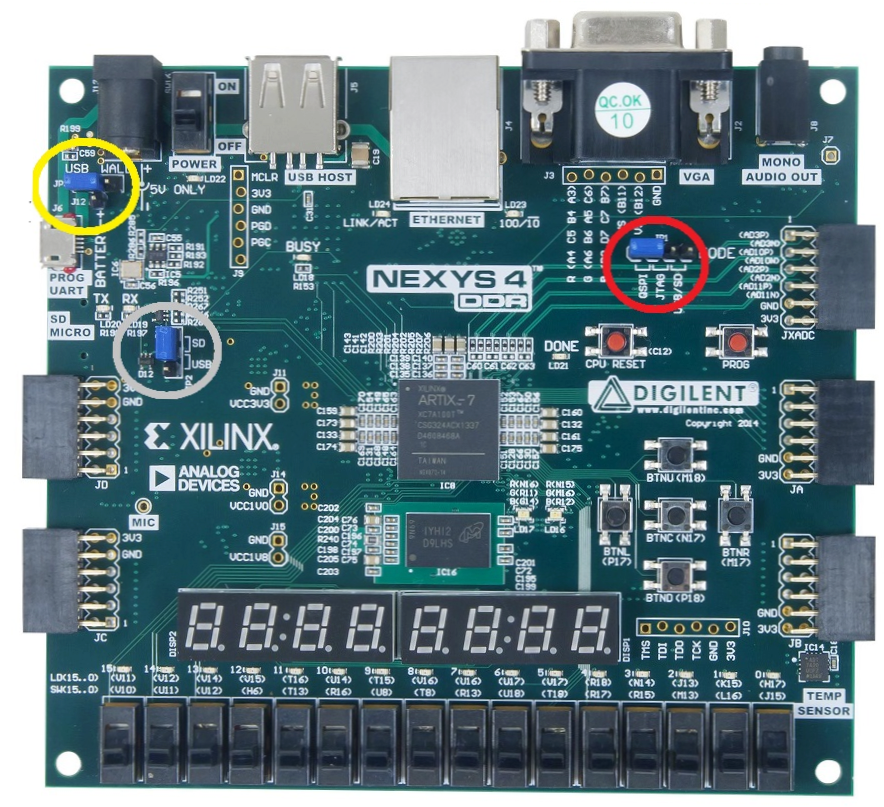
\includegraphics[width=0.9\linewidth]{images/nexys4_jumpers.png}
  \end{center}

The Nexys4 boards can be powered in two ways: using an external power supply, or from a standard USB port.

\subsection{Micro-USB Power}

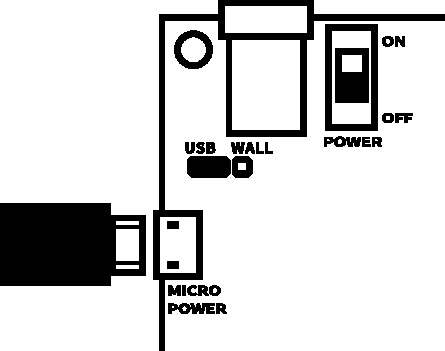
\includegraphics[width=5cm]{images/illustrations/nexys-micro-usb-power.pdf}

Connect your micro-usb cable to a USB port on a USB charger or PC to provide power. Connect the other end to the Nexys4's micro-usb connector. Place the JP3 jumper on pins 1 and 2 to select USB power. Use the switch to power up the Nexys4.

\subsection{External Power Supply}

\hspace*{1.7cm}
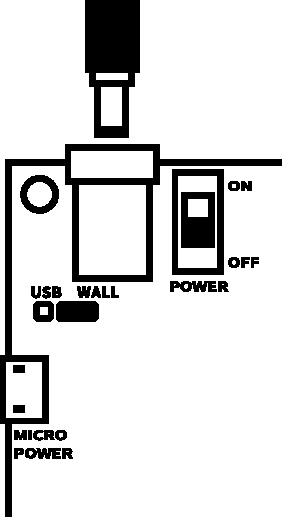
\includegraphics[width=3.2cm]{images/illustrations/nexys-power-supply.pdf}

The MEGA65 core can consume a lot of power, and a standard USB port could potentionally be too little for the Nexys4 board. In particular, writing to the SD card might hang or perform odd behaviour. Therefore you should consider a 5V power supply.

Digilent sell a power supply for the Nexys4 board, and we recommend you use this to ensure you avoid the risk of damage to your Nexys4 board. The chosen power supply should be center positive, 2.1mm internal diameter plug, and should deliver 4.5VDC to 5.5VDC rated at least 1 Amp.

Connect the power supply cable to the supply plug of the Nexys4. Place the JP3 jumper on pins 2 and 3 to select WALL power. Use the switch to power up the Nexys4.

\subsection{Other Jumpers and Switches}

For your initial set up, we'd suggest you set the following jumpers on your Nexys4 board to these positions:

\begin{itemize}
  \item{JP1} - USB/SD
  \item{JP2} - SD
\end{itemize}

\begin{center}
  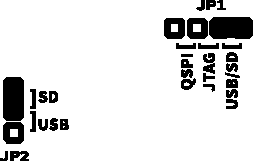
\includegraphics[width=3.2cm]{images/illustrations/nexys-jumpers.pdf}
\end{center}

This will assure that the bitstream files will get loaded from your SD card on start-up.

At some later stage, you may prefer to load the bitstream from the on-board QSPI flash, and at that point, you can revisit your JP1 jumper setting and adjust it to the QSPI position.

% XXX - Image of board highlighting the jumpers

All 16 switches on the lower edge of the board must be set to the off position.


\subsection{Connections and Peripherals}

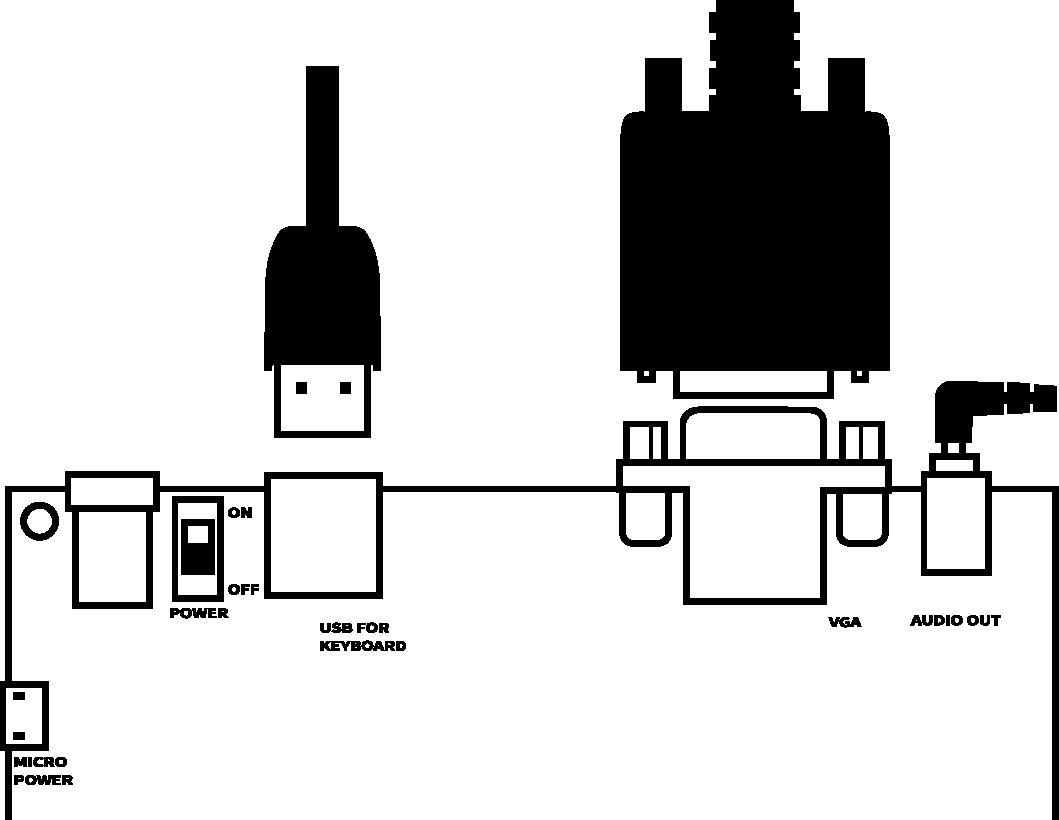
\includegraphics[width=\linewidth]{images/illustrations/nexys-connectors.pdf}

A USB keyboard can be connected to the USB port. Only a keyboard that lacks a USB hub will work with the Nexys4 board.  Generally, extremely cheap keyboards will work, while more expensive keyboards tend to have a USB hub integrated, and will not work.  You may need to try several keyboards before you find one that works.

You can connect a VGA monitor to the VGA port.

The mono audio-out jack can be connected to the line-in of an amplifier.


\subsection{Communicating with your PC}

There may be occasions where you wish to communicate with your Nexys4 board from your PC, in order to perform activities such as:

\begin{itemize}
  \item Flash your QSPI flash chip via Vivado
  \item Upload bitstream files directly from your PC (via m65 tool)
  \item Make use of support tools such as M65Connect, m65, mega65\_ftp, m65dbg, etc
\end{itemize}

On such occasions, you will need to connect your micro-usb cable up to your PC.

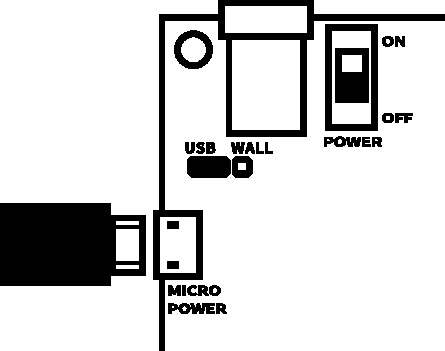
\includegraphics[width=5cm]{images/illustrations/nexys-micro-usb-power.pdf}

\subsection{Onboard buttons}

\begin{center}
  
\includegraphics[width=3.2cm]{images/illustrations/nexys-reset-buttons.pdf}
\end{center}

The ``CPU RESET'' button will reset the MEGA65 when pressed, while the ``PROG'' button will cause the FPGA itself to reload the MEGA65
core.  The main difference between the two is that CPU RESET is faster, and does not clear the contents of memory, while the FPGA button
is slower, and does reset the contents of memory.

\begin{center}
  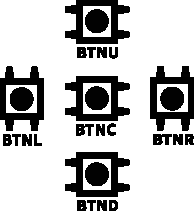
\includegraphics[width=3.2cm]{images/illustrations/nexys-five-buttons.pdf}
\end{center}

Two of the five buttons in the cross arrangement can also be used:  BTND acts as though you have pressed \widekey{RESTORE}, while BTNC will trigger an IRQ, as though the IRQ line had been pulled to ground.

\section{Keyboard}

The keyboard layout is positional rather than logical.
This means that keys in similar positions to the keys on a C65 keyboard will have similar function.
This relationship assumes that your USB keyboard uses a US keyboard layout.

To help you locate what the various MEGA65 keys are mapped to, the MEGA65 has a built-in virtual keyboard test feature. This can be accessed in two ways.

The easiest way is to keep \specialkey{ALT} held down in while switching on the Nexys4, or resetting the Nexys4 with
the ``PROG'' button. The configure menu will be presented and by pressing 3, the virtual keyboard will be presented on a black background.

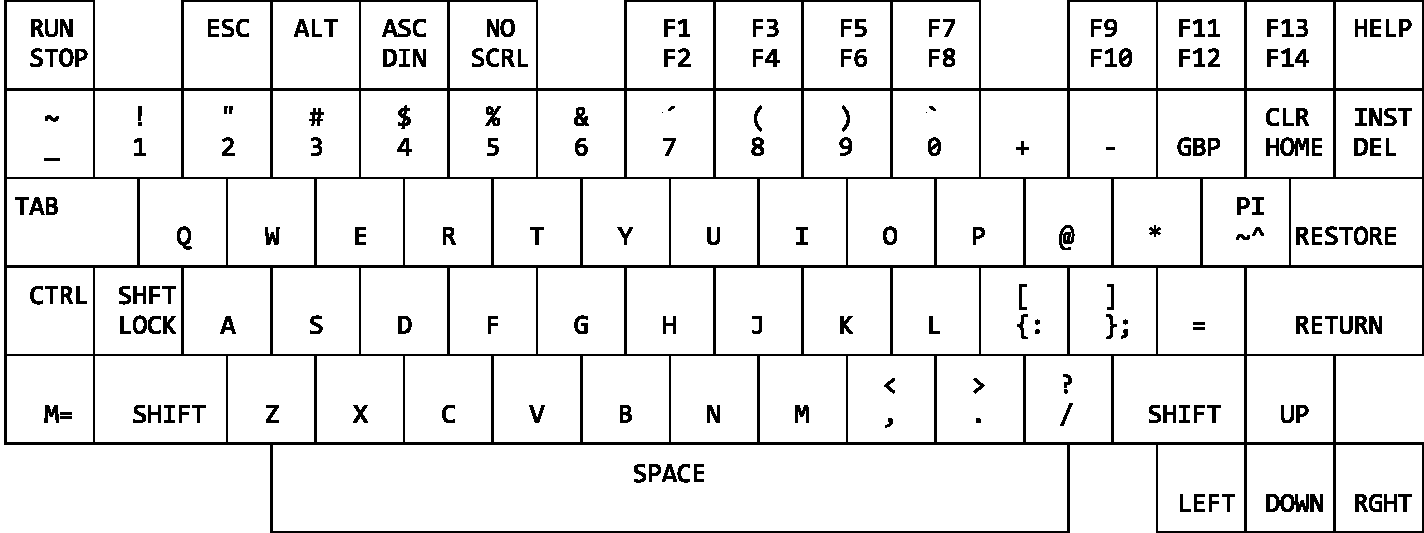
\includegraphics[width=\linewidth]{images/illustrations/virtual-keyboard.pdf}

Pressing a key on the USB keyboard will show the highlighted key on the virtual keyboard to help you identify the key mapping.

The other way to access the virtual keyboard is from within the MEGA65. Hold \megasymbolkey and press \specialkey{TAB} to access the Matrix Mode Debugger. From here, enter the following:

\screentextwide{s ffd3615 ff}

This will open a semi-transparent virtual keyboard at the top of the screen. Alternatively:

\screentextwide{s ffd3615 ff ff}

This will open a semi-transparent virtual keyboard in the centre of the screen.

Hold \megasymbolkey and press \specialkey{TAB} to exit Matrix Mode Debugger and return to the MEGA65.

\subsection{Some key mappings with a USB keyboard}

\widekey{RESTORE} is mapped to the PAGE UP key.

\specialkey{RUN STOP} is mapped to \specialkey{ESC}.

\newpage

\section{Preparing microSDHC card}

The MEGA65 requires an SDHC card of between 4GB and 64GB capacity.  Some SDXC cards may work, however, this is not officially supported.

Preparation steps for the Nexys4 board's SD card share much in common with the steps needed for real MEGA65 hardware, and as such, it is worth having a look over the \nameref{cha:configuring} chapter if you ever need details.

So in this section, we'll provide more details on the distinctive steps, and be more brief on the common steps.

One point of distinction between the Nexys board and the real MEGA65 hardware is that the latter already has a default bitstream/core provided, which permits you to format your SD card in the specific style required by the MEGA65.

For Nexys4 board owners however, you have no such default bitstream, so
see \nameref{sec:bitstreamfiles} for more details on where the appropriate "nexys4.bit" or "nexys4ddr-widget.bit" files for your device can be downloaded from.

\subsection{Preparation Steps}

The steps are:

\begin{itemize}
  \item{Format the SD card} in a convenient computer using the FAT32 file-system.  The MEGA65 and Nexys4 boards do not understand other
file systems, especially the exFAT file system.
\item{Copy} your bitstream file (with name ending in ``.bit'') onto the SD card.
\item{Insert} the SD card into the SD card slot on the under-side of the Nexys4 board.
\item{Switch on} the Nexys4 board.
\item{Enter the Utility Menu} by holding \specialkey{ALT} down on the USB keyboard you have connected to the Nexys4 board.
\item{Enter the FDISK/FORMAT tool} by pressing 2 when the option appears on the MEGA65 boot screen.
\item{Follow the prompts} in the FDISK/FORMAT program to again format the SD card for use by the MEGA65. \\
  \\
  The FDISK tool will partition your SD card into two partitions and format them.
  \begin{itemize}
    \item One is type \$41 = MEGA65 System Partition, where the save slots, configuration data and other files live. \\
  (This partition is invisible in i.e. Win PCs).
    \item The other partition with type \$0C = VFAT32, where KERNAL, support files, games, and so on, will be copied to later. \\
  (This partition is visible on i.e. Win PCs).
  \end{itemize}
\item{Once formatting is complete}, switch off the Nexys4 board and remove the microSDHC card from the Nexys board and put it back into your PC
\item{This time, copy} the following items onto the SD card:
  \begin{itemize}
    \item The bitstream file
    \item The extracted files from within either the "\textbf{SD essentials.rar}" or "\textbf{SD essentialsNoROM.rar}" file that you downloaded from the MEGA65 filehost. (See \nameref{sec:installingrometc} for more details).
    \item{If you have sourced your own preferred ROM file} (e.g. "\textbf{911001.BIN}"), copy it onto the SD card also, and rename it to "\textbf{MEGA65.ROM}" (uppercase is essential).
    \item{Any .D81 disk image files} you wish to make use of.
      \begin{itemize}
        \item Note that if a file named MEGA65.D81 is added to the SD card, it will be mounted automatically on startup.
        \item Make sure that all .D81 files have names that fit the old DOS 8.3 character limit, and are upper case.  This restriction will be removed in a future release.
      \end{itemize}
  \end{itemize}
\item{Remove the SD card} and reinsert it into your Nexys4 board.
\item{Power the Nexys4} board back on.  The MEGA65 should boot within 15 seconds.
\item On first start up, you will find yourself at the on-boarding screen, of which more details can be found in the \nameref{cha:configuring} chapter.

\end{itemize}

Congratulations. Your MEGA65 has been set up and is ready to use.

Please note that the above method of copying the bitstream file to the SD card means that the bitstream is loaded into the Nexys FPGA each time on boot - which takes around 13 seconds for the system to start. The bitstream can also be flashed using Vivado software into the QSPI flash to deliver a boot up time of 0.3 seconds. 

For more detailed information on preparing and configuring your MEGA65, please refer to the \nameref{cha:configuring} chapter. 

\section{Loading the bitstream from QSPI}

While loading the bitstream from the SD card is the suggested (and well-trodden) path this document has chosen, of late, more nexys4 users have been exploring the alternative pathway of loading the bitstream from the QSPI flash. Some potential reasons they have chosen this pathway are:

\begin{itemize}
  \item Faster loading times (0.3 seconds versus 13 seconds)
  \item Some people were interested in the possibility of flashing multiple cores onto their QSPI (via steps described in the \nameref{cha:cores} Chapter)
  \item Some people have experienced niggling issues with the SD card pathway, such as:
    \begin{itemize}
      \item System unable to reboot from on-boarding screen
      \item System unable to reboot from freeze-menu after switching between PAL/NTSC
    \end{itemize}
\end{itemize}

In time, if this proves to be a more popular pathway, we can revise our documentation here to suit it. Here are some steps in brief.

\subsection{Preparation Steps}

For users that want to try this pathway, you will need to adjust the JP1 jumper setting to use QSPI and then follow the steps in the \nameref{cha:fpgacpldflashing} chapter in relation to \nameref{sec:installvivado} and \nameref{sec:mainfpgaflashing}.

Be forewarned that the installation of Vivado is a lengthy process (both in terms of download time, and installation time).

Once you have flashed Slot0 of your QSPI chip via Vivado, you can then follow the steps described in \nameref{cha:configuring} to perform the custom SD card formatting, installing of ROM and support files and on-boarding.

\section{Useful Tips}

The following are some useful tips for getting familiar with the MEGA65:

\begin{itemize}

\item{Press \& hold \megasymbolkey (or the Commodore key if using a Commodore 64 or 65 keyboard) during boot to start up in C64-mode instead of C65-mode}
 \item{Press \& hold \specialkey{RUN STOP} during boot to enter the machine language monitor, instead of starting BASIC.}
\item{Press \widekey{RESTORE} for approximately 1/2 - 1 second to enter the MEGA65 Freeze Menu.  From this menu
  you have convenient tools to change the CPU speed, switch between PAL \& NTSC video mode, change Audio settings, manage freeze-states,
   select D81 disk images, examine and modify memory of the frozen program, among other features.  This is in many ways the heart of the MEGA65, so it is well worth exploring and getting familiar with.}
\item{Type \screentext{POKE0,65} in C64-mode to switch  the CPU to full speed (40MHz). Some software may behave incorrectly in this mode, while other software will work very well, and run many times faster than on a C64.}
\item{Type \screentext{POKE0,64} in C64-mode to switch the CPU to 1MHz.}
\item{Type \screentext{SYS58552} in C64-mode to switch to C65-mode.}
\item{Type \screentext{GO64} in C65-mode and confirm, by pressing \screentext{Y}, to switch to C64-mode, which is the
same as on a C128.}
\item{The C65 ROM makes device 8 the default, so you can normally leave off the \textbf{,8} from the end of LOAD and SAVE commands.}
\item{Pressing \specialkey{SHIFT} + \specialkey{RUN STOP} from either C64 or C65-mode will attempt to boot from disk.}
\end{itemize}

Have fun! The MEGA65 has been lovingly crafted over many years for your enjoyment. We hope you have as much fun using it as we have had creating it!

The MEGA Museum of Electronic Games \& Art welcomes your feedback, suggestions and contributions to this open-source digital heritage preservation project.


\part{CROSS-PLATFORM DEVELOPMENT TOOLS}

\chapter{Emulators}

At the time of writing, there is only one emulator for the MEGA65,\ \stw{xmega65}; LGB's Xemu emulator suite. The LGB developers work hard to keep up with the development of the MEGA65; however, some MEGA65 emulation may not be accurate but should be sufficient for software development on the MEGA65.

% Should there be a link to the LGB suite?

During development, frequently test software on real hardware, such as a MEGA65 or FPGA board capable of running a MEGA65 core.

Download the MEGA65 emulator source code from \url{https://github.com/lgblgblgb/xemu}.

Download pre-compiled versions from \url{https://github.lgb.hu/xemu/}.

A live ISO image containing the emulator, documentation, and other tools is available from \url{Forum64.de}
at \url{https://www.forum64.de/index.php?thread/104698-xemu-live-system-iso-file/\&postID=1549927\#post1549936}.

\section{Using The Xmega65 Emulator}

\section{Using the Live ISO image}

The Live ISO image is the product of a volunteer community; not the MEGA65 team. We include it for your convenience.

\subsection{Creating a Bootable USB stick or DVD}

There are many ways to create a live ISO image. The method you choose depends on your operating system and whether you wish to install to a USB drive or burn it to a DVD. Burning to a DVD is straightforward, assuming you own a computer that has a DVD writer. If you wish to create a faster bootable USB drive, try one of the methods below:

If you are using Windows, consider a tool like \url{http://www.isotousb.com/}.

On Linux, you can use the instructions at \url{https://fossbytes.com/create-bootable-usb-media-from-iso-ubuntu/}.

For Apple Macs, consider these instructions at
\url{https://ubuntu.com/tutorials/create-a-usb-stick-on-macos#1-overview}.

Similar instructions are available for other popular computers, such as Amigas (\url{https://forum.hyperion-entertainment.com/viewtopic.php?t=3857}), or Sun UltraSPARC workstations (\url{https://forums.servethehome.com/index.php?threads/how-to-create-a-bootable-solaris-11-usb.1998/}).

Finally, the popular, easy-to-use, and free cross-platform belanaEtcher is available at \url{https://www.balena.io/etcher/}.

\subsection{Getting Started}

To avoid potential copyright issues, the bootable ISO image does not include proprietary ROMs for the MEGA65; such as legacy C65 ROMs. It does include an open-source replacement ROM from our OpenROMs project.\index{OpenROMs} This ROM will boot into a BASIC 2 environment that you can use to load and execute many C64 programs as shown in the image below:

\screenshotwrap{images/liveiso-openrom.png}

If you wish to use a C65 ROM that includes BASIC 10, download the appropriate ROM file and place it on another USB stick named \stw{MEGA65.ROM}. On start-up, the MEGA65 will ask if a ROM has been downloaded; as shown in the image below:

\screenshotwrap{images/liveiso-rom-usb-prompt.png}

If the Live ISO cannot find a ROM, it will prompt you to download a ROM; as shown below:

\screenshotwrap{images/liveiso-rom-download-prompt.png}

\subsection{Other Features of the Live ISO}

As the previous screen-shots show, the Live ISO provides various and convenient desktop shortcuts. On the left-hand side, there are shortcuts for launching the
MEGA65 emulator and the C65 emulator so you can test that programs
will run on both platforms. As previously mentioned, both emulators are a work in progress and may not be 100\% compatiable.

Another link provides access to the MEGA65 Book. This all-in-one volume, of apporixmately 800 pages, contains the official MEGA65 documentation. The majority of this developer's guide is also present in the MEGA65 Book.

This ISO also includes documentation for the C65 Notepad; a program for the C65 and MEGA65 written by Snoopy (the developer of the Live ISO image). A ``read me'' file contains further information about the Live ISO.

Finally, on the right-hand side, there are links to download a C65 ROM and to update the MEGA65 Book to the latest version. This will ensure you don't need to create a new bootable image each time a frequent update is made to the MEGA65 Book.

To access all contents of the Live ISO image, use the file explorer.

% 2021-03-17 edits by SBC

\chapter{Data Transfer and Debugging Tools}
\label{cha:transfer-and-debug-tools}

The key to effective cross-platform development is having quick and
easy means to deploy and test software on the MEGA65.  This is
especially true while the MEGA65 emulator continues to be developed.
In fact, even once the MEGA65 emulator is complete, it is unlikely
that it will be able to offer full compatibility at full speed,
because the MEGA65 is much more demanding to emulate than the C64.

There are a variety of tools that can be used for data transfer and
debugging.  These typically function using either the MEGA65's serial
monitor interface, or via the MEGA65's fast ethernet adapter.  The
serial monitor interface is available via the UART lines on the JB1
header.

If you do not have access to the serial monitor interface, there are
tools being developed for the fast ethernet port that provide some,
but not all, of the capabilities of the serial monitor
interface. These will be documented as they become available. The
remainder of this chapter focusses on methods that access the serial
monitor interface.

You can either connect a 3.3V UART adaptor to the appropriate
lines, or more conveniently, connect a TE-0790-03 JTAG debug module
onto this connector.  This gives you a USB connection that can be used
for injecting software, remote debugging and memory inspection, as
well as activating or flashing bitstreams.  With this connection,
there are the following tools:

\section{m65 command line tool}

The \url{https://github.com/mega65/mega65-tools} repository contains a
number of tools, utilities and example programs. These tools are mainly for Linux but can be used on Windows with Cygwin. One of those is
the \stw{m65} command line tool. This is rather a swiss-army
knife collection of utilities in one.  Common useful functions
include:

\subsection{Screenshots using m65 tool}

To take a screenshot of the MEGA65 use:

\begin{screenoutput}
m65 -S
\end{screenoutput}

This will create a file called \stw{mega65-screeen-000000.png},
or if that file already exists, the first non-used number will be used
in place of \stw{000000}.

Note that this screenshot function works by having \stw{m65} emulate the
function of the VIC-IV. Thus while it produces excellent looking
digital screenshots, it may not exactly match the real display of the
MEGA65.  At the time of writing it does not render sprites or
bitplanes, only text and bitmap-based video modes.

\subsection{Load and run a program on the MEGA65}

To load and run a program on the MEGA65, you can use a command like:

\begin{screenoutput}
m65 -F -4 -r foo.prg
\end{screenoutput}

The \stw{-F} option tells \stw{m65} to reset the MEGA65
before loading the program.

The \stw{-4} option tells \stw{m65} to switch the MEGA65
to C64-mode before loading the program. If this is left off, then it
will attempt to load the program in C65-mode.

The \stw{-r} option tells \stw{m65} to run the program
immediately after loading.

Note that this command works using the normal BASIC LOAD command, and
is thus limited to loading programs into the lower 64KB of RAM

\subsection{Reconfigure the FPGA to run a different bitstream}

To try out a different MEGA65 bitstream, a command like the following can be
used:

\begin{screenoutput}
m65 -b bitstream.bit
\end{screenoutput}

This will cause the named bitstream to be sent to the FPGA.  As the
FPGA will be reconfigured by this action, and program currently
running will not merely be stopped, but also main memory will be
cleared. For models of the MEGA65 that are fitted with 8MB or 16MB of
expansion memory, those expansion memories are implemented in external
chips, and so the contents of them will not be erased.

For non-MEGA65 bitstreams (such as zxunomega65 and gbc4mega65), use the '-q' argument instead:

\begin{screenoutput}
m65 -q bitstream.bit
\end{screenoutput}

\subsection{Remote keyboard entry}

The MEGA65's keyboard interface logic supports the injection of
synthetic key events using the registers \$D615 -- \$D617.
The \stw{m65} utility uses this to allow remote typing on the MEGA65
in a way that is transparent to software.  There are three ways to use
this:

\begin{screenoutput}
m65 -t sometext
\end{screenoutput}

This form types the supplied text, in this case {\em sometext}, but
does not simulate pressing \specialkey{RETURN}.  If you wish
to simulate the pressing of \specialkey{RETURN}, use \stw{-T}
instead of \stw{-t}, e.g.:

\begin{screenoutput}
m65 -T list
\end{screenoutput}

This would cause the LIST command to be typed and executed.

Finally, it is possible to begin general remote keyboard control via:

\begin{screenoutput}
m65 -t -
\end{screenoutput}

In this mode, any key pressed on the keyboard of the computer
where \stw{m65} is running will be relayed to the MEGA65.  Note that
not all special keys are supported, and that there is some latency, so
using key repeat can cause unexpected results.  But for general remote
control, it is a very helpful facility.

\subsection{Unit testing and logging support}

The \stw{m65} tool includes support to facilitate remote unit testing 
directly on MEGA65 hardware. When \textit{unit testing mode} is active, 
\stw{m65} waits for the MEGA65 to send certain byte sequences over the 
serial interface which signal the current state (started, passed, failed) 
of a given test. Additionally, it is possible to send log messages from 
the MEGA65 to the host computer.

Unit testing mode is entered by calling \stw{m65} with the \stw{-u} flag. 
To run a remote BASIC program in C65-mode and simultaneously put \stw{m65}
into \textit{unit testing mode}, the following command can be used:

\begin{screenoutput}
    m65 -Fur attic-ram.prg -w tests.log
\end{screenoutput}

The \stw{-F} and \stw{-r} options tell \stw{m65} to reset the MEGA65
before loading the program "attic-ram.prg" and then automatically run it. 
The \stw{-u} option then tells \stw{m65} go into \textit{unit testing mode} 
instead of exiting after launching the program.
The optional \stw{-w} option makes \stw{m65} append the test results to the 
file "test.log" (creating the file if it doesn't exist). 

Please note that \stw{m65} automatically exits from \textit{unit testing mode}
if no test state signals were received for over 10 seconds.

Support is provided for sending unit test signals to the host computer from
C and BASIC 65 programs:

\subsubsection{Using unit tests with C}

The MEGA65 libc contains support for unit testing via functions defined in 
\stw{tests.h} and \stw{tests.c}. 

To signal the start of a test, include \stw{tests.h} and use

\begin{verbatim}
    unit_test_setup("testName",issueNumber);
\end{verbatim}

where \textit{"testName"} is a human-readable name of the test (e.g. 
"VIC-II") and \textit{issueNumber} a reference to the corresponding
bug issue (for example, the issue number from github).

After starting a test, it's possible to signal passed tests with 
the unit\_test\_ok() function:

\begin{verbatim}
    unit_test_ok();
\end{verbatim}

A failed test is signalled with unit\_test\_fail():

\begin{verbatim}
    unit_test_fail("fail message");
\end{verbatim}

Each time the unit\_test\_ok() or unit\_test\_fail() 
functions are called, the \textit{sub issue} of the test (reported on 
the host computer) is incremented. This makes it easier to combine and 
identify multiple tests in one file.

You can send arbitrary log messages via unit\_test\_log():

\begin{verbatim}
    unit_test_log("hello world from mega65!");
\end{verbatim}

...and finally, when all is done, the end of unit testing is signalled
by the use of

\begin{verbatim}
    unit_test_done();
\end{verbatim}


\subsubsection{Using unit tests with BASIC 65}

\stw{b65support.bin} is a machine language module providing support for 
unit testing from BASIC 65, available in the \stw{bin65} folder of the mega65-tools
repository. This module works by redirecting the USR vector to perform the functions 
needed to communicate with the testing host.

In an automated test scenario, you may want to inject the \stw{b65support.bin} 
binary into MEGA65 RAM by using \stw{m65}:

    \begin{screenoutput}
        m65 -@ mega65-tools/bin65/b65support.bin@15fe
    \end{screenoutput}


Of course it's also possible to load \stw{b65support.bin} directly from the
MEGA65 by mounting the \stw{M65UTILS.D81} image from the freezer and issuing

\begin{screenoutput}
    BLOAD "B65SUPPORT.BIN"
\end{screenoutput}

After loading, \stw{b65support.bin} is initialized with

\begin{screenoutput}
    SYS $1600
\end{screenoutput}

Once initialized, the following functions are provided by \stw{b65support.bin}:

\begin{screenoutput}
    A=USR(<issueNum>)
\end{screenoutput}
prepares a new test with number <issueNum> and resets subissue number to 0

\begin{screenoutput}
    A=USR("=<testName>")
\end{screenoutput}
sets test name and sends test start signal; for example: \stw{A=USR("=VIC-III")} 
sets the test name to 'VIC-III' and signals the host computer that the test 
has started.

\begin{screenoutput}
    A=USR("/<logMessage>)
\end{screenoutput}
sends a log message to the host computer

\begin{screenoutput}
    A=USR("P")
\end{screenoutput}
sends the 'passed' signal to the host computer and increases the sub issue number

\begin{screenoutput}
    A=USR("F")
\end{screenoutput}
sends the 'test failed' signal to the host computer and increases 
the sub issue number

\begin{screenoutput}
    A=USR("D")
\end{screenoutput}
sends the 'test done' signal to the host computer 

All calls return the current sub issue number or \stw{?ILLEGAL QUANTITY ERROR} in 
case of calling an invalid command.

\subsubsection{BASIC 65 example}

The following is a complete BASIC 65 example showing how to use \stw{m65}'s
unit testing features:

\begin{screenoutput}
    100 rem attic ram cache test
    110 poke $bfffff2,$e0         : rem enable attic ram cache
    120 sys $1600                 : rem init test module
    130 a=usr(379)                : rem set issue number
    140 a=usr("=attic-ram-cache") : rem set test name
    150 bank128:poke0,65          : rem just to be sure
    160 b0=$8000000 : b1=$8000100 : rem attic ram areas to be tested
    170 for r=0 to $ff
    180   poke b0+r,0             : rem fill area 1 with 0
    190   poke b1+r,$ff           : rem fill area 2 with $ff
    200 next r
    210 for t=1 to 10             : rem 10 tries
    220   poke b0,32              : rem write to b0
    230   for x=0 to $ff:t1=b1+x
    240     a=peek(b0)            : rem read from b0
    250     b=peek(t1):b=peek(t1) : rem read twice from t1
    260     ifb<>255 thenf=t:t=11:x=256   : rem this shouldn't happen
    270   next x
    280 next t
    290 if f=0 then begin
    300   print "no faults detected after";t;"tries."
    310   a=usr("p")              : rem signal 'test passed' to host
    320 bend : else begin
    330   a=usr("f")              : rem signal 'test failed' to host
    340   print "hyper ram fault detected after";f;"tries."
    350   print "peek($";hex$(t1);") [t1] is";b;"but should be 255"
    360 bend
    370 a=usr("d")                : rem test done    
\end{screenoutput}

\section{M65Connect}

This is a cross-platform graphical tool available for Windows, Linux
and MacOSX, which allows access to most of the functions of
the \stw{m65} command-line tool, without needing to use a
command line, or being able to compile the tool for your preferred
operating system.

The repository for M65Connect is: \url{https://github.com/MEGA65/m65connect}

The latest binary version is available from \url{https://files.mega65.org}.

With the MEGA65 or Nexys FPGA switched off, connect a USB cable from your computer to the MEGA65 or Nexys FPGA board. Run the \textit{M65Connect} executable and follow the prompts to connect. The program will help you identify which USB Serial Port to communicate over.

With this tool you can easily transfer PRG programs and a variety of other files. M65Connect can handle the transfer, switching to C64-mode, and execution of programs.

\section{mega65\_ftp}

The \stw{mega65}\_\stw{ftp} utility from
the \url{https://github.com/mega65/mega65-tools} repository is a
little misleadingly named: While it 
is a File Transfer Program, it does not use the File Transfer
Protocol (FTP).  Rather, it uses the serial monitor interface to take
remote control of a MEGA65, and directly access its SD card to enable
copying of files between the MEGA65 and the host computer.

Note that it does not perfectly restore the MEGA65's state on exit,
and thus should only be used when the MEGA65 is at the READY prompt,
so that any running software doesn't go haywire. In particular, you
should avoid using it when a sensitive program is running, such as
the Freeze Menu, MEGA65 Configuration Utility, or the MEGA65
Format/FDISK utility.  (This problem could be solved with a little
effort, if someone has the time and interest to fix it).

When run, it provides an FTP-like interface that supports
the \stw{get}, \stw{put}, \stw{rename} and \stw{dir} commands.
Note that when putting a file, you should make sure that it is given a
name that is all capitals and has o DOS-compatible 8.3 character file
name.  This is due to limitations in both \stw{mega65}\_\stw{ftp} and the
MEGA65's Hypervisor's VFAT32 file system code. Again, these problems
could be fixed with a modest amount of effort on the part of a
motivated member of the community.

Finally, the \stw{mega65}\_\stw{ftp} program is {\em very} slow to push
new files to the MEGA65, typically yielding speeds of around 5KB/sec.
This is partly because the serial monitor interface is capable of
transferring data at only 40KB/sec (when set to 4,000,000 bits per
second), and partly because the remote control process results in a
lot of round-trips where helper routines are executed on the MEGA65 to
read, write and verify sectors on the SD card.  It would be quite
feasible to improve this to reach close to 40KB/sec, and potentially
faster using either some combination of data compression,
de-duplication of identical sectors (especially when uploading disk
images) and other techniques. Again, this would be a very welcome
contribution that someone in the community could contribute to
everyone's benefit.

\section{TFTP Server}

Work on a true TFTP server for the MEGA65 that supports fast
TFTP transfers over the 100mbit ethernet has begun, and can be used to
very quickly read files from the MEGA65. Speeds of close to 1MB/sec
are possible, depending on SD card performance.  Rather than using
DHCP, this utility will respond to {\em any} IP address that ends in
.65. It always uses the MAC address 40:40:40:40:40:40. True DHCP
support as well as using the MEGA65's configured ethernet MAC address
may be added in the future. 

More importantly, support for writing
files to the SD card is not yet complete, and is blocked by the need
for the implementation of the necessary functions in the MEGA65's Hypervisor for creating and
growing files.  A particular challenge is enabling the creation of
files with contiguous clusters as is required for D81 disk images: If
a D81 file is fragmented, then it cannot be mounted, because the
mounting mechanism requires a pointer to the contiguous block of the
SD card containing the disk image.
In the interim, \stw{mega65}\_\stw{ftp} can be used as a substitute.

\section{Converting a BASIC text file listing into a PRG file}

If you have a untokenised BASIC program in plain text format sourced from somewhere like an internet post, and you wish to try it on the MEGA65 without typing it in, it is possible to convert it to a PRG.

\textit{C64List} is a Windows-based command-line tool that will allow you to make the conversion. Once you have a \textit{.PRG} file, you can use a tool like M65Connect to upload it to the MEGA65 or Nexys FPGA. 

C64List is available for download from \url{http://www.commodoreserver.com/Downloads.asp}

Ensure you have a program listing saved to a file on your local computer (for example, \textit{program.txt}) encoded as ANSI or UTF8.

Use C64List to convert the file to a PRG file using:
    
\begin{tcolorbox}[colback=black,coltext=white]
    \begin{verbatim}
        C64List program.txt -prg
    \end{verbatim}
\end{tcolorbox}

Now you can upload your newly converted program to the MEGA65 with M65Connect or one of the other tools described previously.

It is worth noting that this method will not be 100\% effective on listings with special PETSCII characters. Programs with PETSCII will require some editing on the MEGA65 itself before saving to disk.

\chapter{Assemblers}

The short answer is that we recommend that you use the ACME
assembler.  The mnemonics used by ACME are now considered the official
onces for the 45GS02.  KickAsm is also quite suitable. The long answer continues below.

There are any number of assemblers that can be used to develop for the
MEGA65.  However only very few support the MEGA65's advanced CPU
features, or even the C65 4510 instructions.

Four different
assemblers have been used for different parts of the MEGA65 software,
reflecting the rather haphazard history of developing assembler
support for the MEGA65.  The first assembler to support the MEGA65 was
{\bf Ophis}, as it seemed the easiest to patch.  {\bf KickAss} later gained
support, followed by ACME. {\bf ACME} added support at a convenient time, when
the extended instructions, their names and syntax had sufficiently stabilised.

From the perspective of the MEGA65 team, ACME has two advantages over KickAsm:
First, it is open source, which fits the ethos of the project, and ensures long-term
availability. Second, it is written in C, rather than Java, which means that
it may be possible to port to run natively on the MEGA65 at some point in
the future.

Our fork of {\bf CA65} (\url{https://github.com/mega65/cc65}), the assembler
used in CC65, also now has the ability
to detect the MEGA65's CPU, but has no explicit support for the
processor's features.  This is an important fix, however, as otherwise
software using the CC65 processor detection routine thinks that the
MEGA65 has a 65816, which can result in the execution of incompatible
instructions. This causes problems with Synthmark64 0.2, for example.

Bit Shifter's Assembler {\bf BSA} also supports the 45GS02.  The source
for this assembler can be found at \url{https://github.com/Edilbert/BSA}.

The {\bf BSA} Assembler is currently used for the assembly of the source code
of the {\bf MEGA65.ROM}. Most of this source code is written in the syntax
of the ancient {\bf BSO} assembler (Boston Systems Office), which was used in the
years 1989 - 1991 by software developers, working on the C65.
The {\bf BSA} Assembler has a compatibility mode, which makes it
possible to assemble these old source codes with minor or none modifications.
The {\bf BSA} Assembler has currently only a description of commands
embedded in the C-source of the assembler.

Therefore a chapter, describing the usage and the features of {\bf BSA}
is started after this chapter and will be completed during the next weeks.


\chapter{C and C-Like Compilers}

Short answer: CC65 and KickC both work on the MEGA65.

Both CC65 and KickC are known to work on the MEGA65.  However, both by
default have only a C64 memory model, and use only 6502 opcodes.
It would be super for someone to create a C65 memory configuration for
CC65, and should not be too hard to do.

CC65 supports overlays, which
could be powerfully used with the MEGA65's extra memory to allow
programmes larger than 64KB.  However, this would require writing a
suitable loader for such programmes, which also does not yet exist.

Similarly, modifying the code
generator of CC65 to use 45GS02 features would not be particularly
difficult to do, and would help to overcome the otherwise horribly
slow and bloated code that CC65 produces.  Also adding first-class
support for the 45GS02 CPU features in CA65 (or perhaps even better,
making CC65 produce ACME compatible assembly output) would be of
tremendous advantage, and not particularly hard to do.  These would
all be great tasks to tackle while you wait for your MEGA65 DevKit to
arrive! 


\chapter{MEGA65 Standard C Library}

A C library is being developed for the MEGA65, and which already
includes a number of useful features. This library is available from
\url{http://github.com/mega65/mega65-libc}. The procedures,
functions and definitions it provides are documented in a separate
chapter.

The MEGA65 libc is currently available only for CC65, although we would
welcome someone maintaining a KickC port of it.

\section{Structure and Usage}

The MEGA65 libc is purposely provided in source-form only, and with groups
of functions in separate files, and with separate header files for including.
The idea is that you include only the header files that you require, and
add only the source files required to the list of source files of the programme
you are compiling.  This avoids the risk of the compiler including functions
in your compiled programme that are never used, and thus wasting precious memory
space.

Note that some library source files are written in C, and thus are present as
files with a \stw{.c} extension, while others are written in assembly language
either for efficiency or out of necessity, and have a \stw{.s} extension.

Typical usage is to either have the mega65-libc source code checked out in an
adjacent directory, or within the source directory of your own project.  In the
latter case, this can be done using the git submodule facility.

The following sections document each of the header files and the corresponding
functions that they provide.

\section{conio.h}


\subsection{conionit}
\index{conionit}
\begin{description}[leftmargin=2cm,style=nextline]
\item [Description:] {Initializes the library internal state}
\item [Syntax:] \stw{void conioinit(void)}
\item [Notes:] {This must be called before using any conio library function.}
\end{description}

\subsection{setscreenaddr}
\index{setscreenaddr}
\begin{description}[leftmargin=2cm,style=nextline]
\item [Description:] {Sets the screen RAM start address}
\item [Syntax:] \stw{void setscreenaddr(long addr);}
\item [Parameters:]
\begin{description}\item[]
\item [{\em addr}:] {The address to set as start of screen RAM}
\end{description}
\item [Notes:] {No bounds check is performed on the selected address}
\end{description}

\subsection{getscreenaddr}
\index{getscreenaddr}
\begin{description}[leftmargin=2cm,style=nextline]
\item [Description:] {Returns the screen RAM start address}
\item [Syntax:] \stw{long getscreenaddr(void);}
\item [Desription:] {The current screen RAM address start address.}
\end{description}

\subsection{clrscr}
\index{clrscr}
\begin{description}[leftmargin=2cm,style=nextline]
\item [Description:] {Clear the text screen. }
\item [Syntax:] \stw{void clrscr(void)}
\item [Notes:] {Color RAM will be cleared with current text color}
\end{description}

\subsection{getscreensize}
\index{getscreensize}
\begin{description}[leftmargin=2cm,style=nextline]
\item [Description:] {Returns the dimensions of the text screen}
\item [Syntax:] \stw{void getscreensize(unsigned char* width, unsigned char* height)}
\item [Parameters:]
\begin{description}\item[]
\item [{\em width}:] {Pointer to location where width will be returned}
\item [{\em width}:] {Pointer to location where height will be returned}
\end{description}
\end{description}

\subsection{setscreensize}
\index{setscreensize}
\begin{description}[leftmargin=2cm,style=nextline]
\item [Description:] {Sets the dimensions of the text screen}
\item [Syntax:] \stw{void setscreensize(unsigned char width, unsigned char height)}
\item [Parameters:]
\begin{description}\item[]
\item [{\em width}:] {The width in columns (40 or 80)}
\item [{\em width}:] {The height in rows (25 or 50)}
\end{description}
\item [Notes:] {Currently only 40/80 and 25/50 are accepted. Other values are ignored.}
\end{description}

\subsection{set16bitcharmode}
\index{set16bitcharmode}
\begin{description}[leftmargin=2cm,style=nextline]
\item [Description:] {Sets or clear the 16-bit character mode}
\item [Syntax:] \stw{void set16bitcharmode(unsigned char f)}
\item [Parameters:]
\begin{description}\item[]
\item [{\em f}:] {Set true to set the 16-bit character mode}
\end{description}
\end{description}

\subsection{setextendedattrib}
\index{setextendedattrib}
\begin{description}[leftmargin=2cm,style=nextline]
\item [Description:] {Sets or clear the VIC-III extended attributes mode to support blink, underline, bold and highlight.}
\item [Syntax:] \stw{void setextendedattrib(unsigned char f)}
\item [Parameters:]
\begin{description}\item[]
\item [{\em f}:] {Set true to set the extended attributes mode}
\end{description}
\end{description}

\subsection{togglecase}
\index{togglecase}
\begin{description}[leftmargin=2cm,style=nextline]
\item [Description:] {Toggle the current character set case}
\item [Syntax:] \stw{void togglecase(void)}
\end{description}

\subsection{bordercolor}
\index{bordercolor}
\begin{description}[leftmargin=2cm,style=nextline]
\item [Description:] {Sets the current border color}
\item [Syntax:] \stw{void bordercolor(unsigned char c)}
\item [Parameters:]
\begin{description}\item[]
\item [{\em c}:] {The color to set}
\end{description}
\end{description}

\subsection{bgcolor}
\index{bgcolor}
\begin{description}[leftmargin=2cm,style=nextline]
\item [Description:] {Sets the current screen (background) color}
\item [Syntax:] \stw{void bgcolor(unsigned char c)}
\item [Parameters:]
\begin{description}\item[]
\item [{\em c}:] {The color to set}
\end{description}
\end{description}

\subsection{textcolor}
\index{textcolor}
\begin{description}[leftmargin=2cm,style=nextline]
\item [Description:] {Sets the current text color}
\item [Syntax:] \stw{void textcolor(unsigned char c)}
\item [Parameters:]
\begin{description}\item[]
\item [{\em c}:] {The color to set}
\end{description}
\end{description}

\subsection{revers}
\index{revers}
\begin{description}[leftmargin=2cm,style=nextline]
\item [Description:] {Enable the reverse attribute}
\item [Syntax:] \stw{void revers(unsigned char c)}
\item [Parameters:]
\begin{description}\item[]
\item [{\em enable}:] {0 to disable, 1 to enable}
\end{description}
\item [Notes:] {Extended attributes mode must be active. See setextendedattrib.}
\end{description}

\subsection{highlight}
\index{highlight}
\begin{description}[leftmargin=2cm,style=nextline]
\item [Description:] {Enable the highlight attribute}
\item [Syntax:] \stw{void highlight(unsigned char c)}
\item [Parameters:]
\begin{description}\item[]
\item [{\em enable}:] {0 to disable, 1 to enable}
\end{description}
\item [Notes:] {Extended attributes mode must be active. See setextendedattrib.}
\end{description}

\subsection{blink}
\index{blink}
\begin{description}[leftmargin=2cm,style=nextline]
\item [Description:] {Enable the blink attribute}
\item [Syntax:] \stw{void blink(unsigned char c)}
\item [Parameters:]
\begin{description}\item[]
\item [{\em enable}:] {0 to disable, 1 to enable}
\end{description}
\item [Notes:] {Extended attributes mode must be active. See setextendedattrib.}
\end{description}

\subsection{underline}
\index{underline}
\begin{description}[leftmargin=2cm,style=nextline]
\item [Description:] {Enable the underline attribute}
\item [Syntax:] \stw{void underline(unsigned char c)}
\item [Parameters:]
\begin{description}\item[]
\item [{\em enable}:] {0 to disable, 1 to enable}
\end{description}
\item [Notes:] {Extended attributes mode must be active. See setextendedattrib.}
\end{description}

\subsection{cellcolor}
\index{cellcolor}
\begin{description}[leftmargin=2cm,style=nextline]
\item [Description:] {Sets the color of a character cell}
\item [Syntax:] \stw{void cellcolor(unsigned char x, unsigned char y, unsigned char c)}
\item [Parameters:]
\begin{description}\item[]
\item [{\em x}:] {The cell X-coordinate}
\item [{\em y}:] {The cell Y-coordinate}
\item [{\em c}:] {The color to set}
\end{description}
\item [Notes:] {No screen bounds checks are performed; out of screen behavior is undefined }
\end{description}

\subsection{fillrect}
\index{fillrect}
\begin{description}[leftmargin=2cm,style=nextline]
\item [Description:] {Fill a rectangular area with character and color value}
\item [Syntax:] \stw{void fillrect(const RECT *rc, unsigned char ch, unsigned char col)}
\item [Parameters:]
\begin{description}\item[]
\item [{\em rc}:] {A RECT structure specifying the box coordinates}
\item [{\em ch}:] {A char code to fill the rectangle}
\item [{\em col}:] {The color to fill}
\end{description}
\item [Notes:] {No screen bounds checks are performed; out of screen behavior is undefined }
\end{description}

\subsection{box}
\index{box}
\begin{description}[leftmargin=2cm,style=nextline]
\item [Description:] {Draws a box with graphic characters}
\item [Syntax:] \stw{void box(const RECT *rc, unsigned char color, unsigned char style, unsigned char clear, unsigned char shadow)}
\item [Parameters:]
\begin{description}\item[]
\item [{\em rc}:] {A RECT structure specifying the box coordinates}
\item [{\em color}:] {The color to use for the graphic characters}
\item [{\em style}:] {The style for the box borders. Can be set to BOX\_STYLE\_ROUNDED, BOX\_STYLE\_INNER, BOX\_STYLE\_OUTER, BOX\_STYLE\_MID }
\item [{\em clear}:] {Set to 1 to clear the box interior with the selected color}
\item [{\em shadow}:] {Set to 1 to draw a drop shadow}
\end{description}
\item [Notes:] {No screen bounds checks are performed; out of screen behavior is undefined }
\end{description}

\subsection{hline}
\index{hline}
\begin{description}[leftmargin=2cm,style=nextline]
\item [Description:] {Draws an horizontal line.}
\item [Syntax:] \stw{void hline(unsigned char x, unsigned char y, unsigned char len, unsigned char style)}
\item [Parameters:]
\begin{description}\item[]
\item [{\em x}:] {The line start X-coordinate}
\item [{\em y}:] {The line start Y-coordinate}
\item [{\em len}:] {The line length}
\item [{\em style}:] {The style for the line. See HLINE\_ constants for available styles. }
\end{description}
\item [Notes:] {No screen bounds checks are performed; out of screen behavior is undefined }
\end{description}

\subsection{vline}
\index{vline}
\begin{description}[leftmargin=2cm,style=nextline]
\item [Description:] {Draws a vertical line.}
\item [Syntax:] \stw{void vline(unsigned char x, unsigned char y, unsigned char len, unsigned char style)}
\item [Parameters:]
\begin{description}\item[]
\item [{\em x}:] {The line start X-coordinate}
\item [{\em y}:] {The line start Y-coordinate}
\item [{\em len}:] {The line length}
\item [{\em style}:] {The style for the line. See VLINE\_ constants for available styles. }
\end{description}
\item [Notes:] {No screen bounds checks are performed; out of screen behavior is undefined }
\end{description}

\subsection{gohome}
\index{gohome}
\begin{description}[leftmargin=2cm,style=nextline]
\item [Description:] {Set the current position at home (0,0 coordinate)}
\item [Syntax:] \stw{void gohome(void)}
\end{description}

\subsection{gohome}
\index{gohome}
\begin{description}[leftmargin=2cm,style=nextline]
\item [Description:] {Set the current position at X,Y coordinates}
\item [Syntax:] \stw{void gotoxy(unsigned char x, unsigned char y)}
\item [Parameters:]
\begin{description}\item[]
\item [{\em x}:] {The new X-coordinate}
\item [{\em y}:] {The new Y-coordinate}
\end{description}
\item [Notes:] {No screen bounds checks are performed; out of screen behavior is undefined }
\end{description}

\subsection{gotox}
\index{gotox}
\begin{description}[leftmargin=2cm,style=nextline]
\item [Description:] {Set the current position X-coordinate}
\item [Syntax:] \stw{void gotox(unsigned char x)}
\item [Parameters:]
\begin{description}\item[]
\item [{\em x}:] {The new X-coordinate}
\end{description}
\item [Notes:] {No screen bounds checks are performed; out of screen behavior is undefined }
\end{description}

\subsection{gotoy}
\index{gotoy}
\begin{description}[leftmargin=2cm,style=nextline]
\item [Description:] {Set the current position Y-coordinate}
\item [Syntax:] \stw{void gotoy(unsigned char y)}
\item [Parameters:]
\begin{description}\item[]
\item [{\em y}:] {The new Y-coordinate}
\end{description}
\item [Notes:] {No screen bounds checks are performed; out of screen behavior is undefined }
\end{description}

\subsection{moveup}
\index{moveup}
\begin{description}[leftmargin=2cm,style=nextline]
\item [Description:] {Move current position up}
\item [Syntax:] \stw{void moveup(unsigned char count)}
\item [Parameters:]
\begin{description}\item[]
\item [{\em count}:] {The number of positions to move}
\end{description}
\item [Notes:] {No screen bounds checks are performed; out of screen behavior is undefined }
\end{description}

\subsection{movedown}
\index{movedown}
\begin{description}[leftmargin=2cm,style=nextline]
\item [Description:] {Move current position down}
\item [Syntax:] \stw{void movedown(unsigned char count)}
\item [Parameters:]
\begin{description}\item[]
\item [{\em count}:] {The number of positions to move}
\end{description}
\item [Notes:] {No screen bounds checks are performed; out of screen behavior is undefined }
\end{description}

\subsection{moveleft}
\index{moveleft}
\begin{description}[leftmargin=2cm,style=nextline]
\item [Description:] {Move current position left}
\item [Syntax:] \stw{void moveleft(unsigned char count)}
\item [Parameters:]
\begin{description}\item[]
\item [{\em count}:] {The number of positions to move}
\end{description}
\item [Notes:] {No screen bounds checks are performed; out of screen behavior is undefined }
\end{description}

\subsection{moveright}
\index{moveright}
\begin{description}[leftmargin=2cm,style=nextline]
\item [Description:] {Move current position right}
\item [Syntax:] \stw{void moveright(unsigned char count)}
\item [Parameters:]
\begin{description}\item[]
\item [{\em count}:] {The number of positions to move}
\end{description}
\item [Notes:] {No screen bounds checks are performed; out of screen behavior is undefined }
\end{description}

\subsection{wherex}
\index{wherex}
\begin{description}[leftmargin=2cm,style=nextline]
\item [Description:] {Return the current position X coordinate}
\item [Syntax:] \stw{unsigned char wherex(void)}
\item [Desription:] {The current position X coordinate}
\end{description}

\subsection{wherey}
\index{wherey}
\begin{description}[leftmargin=2cm,style=nextline]
\item [Description:] {Return the current position Y coordinate}
\item [Syntax:] \stw{unsigned char wherey(void)}
\item [Desription:] {The current position Y coordinate}
\end{description}

\subsection{cputc}
\index{cputc}
\begin{description}[leftmargin=2cm,style=nextline]
\item [Description:] {Output a single character to screen at current position}
\item [Syntax:] \stw{void cputc(unsigned char c)}
\item [Parameters:]
\begin{description}\item[]
\item [{\em c}:] {The character to output}
\end{description}
\end{description}

\subsection{cputnc}
\index{cputnc}
\begin{description}[leftmargin=2cm,style=nextline]
\item [Description:] {Output N copies of a character at current position}
\item [Syntax:] \stw{void cputnc(unsigned char count, unsigned char c)}
\item [Parameters:]
\begin{description}\item[]
\item [{\em c}:] {The character to output}
\item [{\em count}:] {The count of characters to print}
\end{description}
\end{description}

\subsection{cputhex}
\index{cputhex}
\begin{description}[leftmargin=2cm,style=nextline]
\item [Description:] {Output an hex-formatted number at current position}
\item [Syntax:] \stw{void cputhex(long n, unsigned char prec)}
\item [Parameters:]
\begin{description}\item[]
\item [{\em n}:] {The number to write}
\item [{\em prec}:] {The precision of the hex number, in digits. Leading zeros will be printed accordingly}
\end{description}
\item [Notes:] {The \$ symbol will be automatically added at beginning of string}
\end{description}

\subsection{cputdec}
\index{cputdec}
\begin{description}[leftmargin=2cm,style=nextline]
\item [Description:] {Output a decimal number at current position}
\item [Syntax:] \stw{void cputdec(long n, unsigned char padding, unsigned char leadingZ)}
\item [Parameters:]
\begin{description}\item[]
\item [{\em n}:] {The number to write}
\item [{\em padding}:] {The padding space to add before number}
\item [{\em leadingZ}:] {The leading zeros to print}
\end{description}
\end{description}

\subsection{cputs}
\index{cputs}
\begin{description}[leftmargin=2cm,style=nextline]
\item [Description:] {Output a string at current position}
\item [Syntax:] \stw{void cputs(const char* s)}
\item [Parameters:]
\begin{description}\item[]
\item [{\em s}:] {The string to print}
\end{description}
\item [Notes:] {No pointer check is performed.  If s is null or invalid, behavior is undefined }
\end{description}

\subsection{cputsxy}
\index{cputsxy}
\begin{description}[leftmargin=2cm,style=nextline]
\item [Description:] {Output a string at X,Y coordinates}
\item [Syntax:] \stw{void cputsxy (unsigned char x, unsigned char y, const char* s)}
\item [Parameters:]
\begin{description}\item[]
\item [{\em s}:] {The string to print}
\item [{\em x}:] {The X coordinate where string will be printed}
\item [{\em y}:] {The Y coordinate where string will be printed}
\end{description}
\item [Notes:] {No pointer check is performed.  If s is null or invalid, behavior is undefined }
\end{description}

\subsection{cputcxy}
\index{cputcxy}
\begin{description}[leftmargin=2cm,style=nextline]
\item [Description:] {Output a single character at X,Y coordinates}
\item [Syntax:] \stw{void cputcxy (unsigned char x, unsigned char y, unsigned char c)}
\item [Parameters:]
\begin{description}\item[]
\item [{\em x}:] {The X coordinate where character will be printed}
\item [{\em y}:] {The Y coordinate where character will be printed}
\item [{\em c}:] {The character to print}
\end{description}
\end{description}

\subsection{cputncxy}
\index{cputncxy}
\begin{description}[leftmargin=2cm,style=nextline]
\item [Description:] {Output N copies of a single character at X,Y coordinates}
\item [Syntax:] \stw{void cputncxy (unsigned char x, unsigned char y, unsigned char c)}
\item [Parameters:]
\begin{description}\item[]
\item [{\em x}:] {The X coordinate where character will be printed}
\item [{\em y}:] {The Y coordinate where character will be printed}
\item [{\em count}:] {The number of characters to output}
\item [{\em c}:] {The character to print}
\end{description}
\end{description}

\subsection{cprintf}
\index{cprintf}
\begin{description}[leftmargin=2cm,style=nextline]
\item [Description:] {Prints formatted output.

    Escape strings can be used to modify attributes, move cursor,etc,
    similar to PRINT in CBM BASIC. Available escape codes:

    Cursor positioning

    \textbackslash t           Go to next tab position (multiple of 8s) \\
    \textbackslash r           Return \\
    \textbackslash n           New-line (assume \textbackslash r like in C printf)

    {clr}
}
\item [Syntax:] \stw{unsigned char cprintf (const unsigned char* format, ...)}
\item [Parameters:]
\begin{description}\item[]
\item [{\em format}:] {The string to output. See escape codes for formatting options.}
\end{description}
\item [Notes:] {Currently no argument replacement is done with the variable arguments.}
\end{description}

\subsection{cgetc}
\index{cgetc}
\begin{description}[leftmargin=2cm,style=nextline]
\item [Description:] { Waits until a character is in the keyboard buffer and returns it }
\item [Syntax:] \stw{unsigned char cgetc (void);}
\item [Desription:] {The last character in the keyboard buffer }
\item [Notes:] {Returned values are ASCII character codes}
\end{description}

\subsection{kbhit}
\index{kbhit}
\begin{description}[leftmargin=2cm,style=nextline]
\item [Description:] { Returns the character in the keyboard buffer }
\item [Syntax:] \stw{unsigned char kbhit (void);}
\item [Desription:] {The character code in the keyboard buffer,  0 otherwise. }
\item [Notes:] {Returned values are ASCII character codes}
\end{description}

\subsection{getkeymodstate}
\index{getkeymodstate}
\begin{description}[leftmargin=2cm,style=nextline]
\item [Description:] {
   Return the key modifiers state, where bits:

    Bit           Meaning             Constant
    ----------------------------------------------------
    0             Right SHIFT state   KEYMOD\_RSHIFT
    1             Left  SHIFT state   KEYMOD\_LSHIFT
    2             CTRL state          KEYMOD\_CTRL
    3             MEGA/C= state       KEYMOD\_MEGA
    4             ALT state           KEYMOD\_ALT
    5             NOSCRL state        KEYMOD\_NOSCRL
    6             CAPSLOCK state      KEYMOD\_CAPSLOCK
    7             Reserved            -
    }
\item [Syntax:] \stw{unsigned char getkeymodstate(void)}
\item [Desription:] {A byte with the key modifier state bits.}
\end{description}

\subsection{flushkeybuf}
\index{flushkeybuf}
\begin{description}[leftmargin=2cm,style=nextline]
\item [Description:] {Flush the keyboard buffer}
\item [Syntax:] \stw{void flushkeybuf(void)}
\end{description}

\subsection{cinput}
\index{cinput}
\begin{description}[leftmargin=2cm,style=nextline]
\item [Description:] {Get input from keyboard, printing incoming characters at current position.}
\item [Syntax:] \stw{unsigned char cinput(char* buffer, unsigned char buflen, unsigned char flags)}
\item [Parameters:]
\begin{description}\item[]
\item [{\em buffer}:] {Target character buffer preallocated by caller}
\item [{\em buflen}:] {Target buffer length in characters}
\item [{\em flags}:] {Flags for input:  (default is accept all printable characters)

            CINPUT\_ACCEPT\_NUMERIC
            CINPUT\_ACCEPT\_LETTER
            CINPUT\_ACCEPT\_SYM
            CINPUT\_ACCEPT\_ALL
            CINPUT\_ACCEPT\_ALPHA
  }
\end{description}
\item [Desription:] {Successfully read characters in buffer}
\end{description}



\subsection{VIC\_BASE}

{\em VIC\_BASE} is a pre-processor macro that provides the base address of the
VIC-IV chip, i.e., \$D000.

{\em IS\_H640} is a pre-processor macro that returns 0 if the current VIC-III/IV
video mode is set to 320 pixels accross (40 column mode), and non-zero if it is set to 640 pixels across (80 column mode).

\chapter{BASIC Tokenisers}

Various tokenisers for C64 BASIC exist, e.g., \url{https://github.com/catseye/hatoucan},
\url{https://www.c64-wiki.com/wiki/C64list}, or the \stw{petcat} utility that is part of VICE.
If you are using Ubuntu Linux, you can install \stw{petcat} by using the following command:

\begin{screenoutput}
sudo apt-get install vice
\end{screenoutput}

We recommend \stw{petcat}, because it supports both C64 BASIC 2 and C65 BASIC 10.



\part{APPENDICES}

\begin{appendices}

  \chapter{Accessories}


  \def\drivedefinition{
{\bf drive} drive \# in dual drive disk units. \\
The drive \# defaults to {\bf 0} and can be omitted on single drive units
such as the 1541, 1571, or 1581.
}

\def\unitdefinition{
{\bf unit} device number on the IEC bus.
Typically in the range from 8 to 11 for disk units.
If a variable is used, it must be placed in brackets.
The unit \# defaults to {\bf 8}.
}

\def\filenamedefinition{
{\bf filename} is either a quoted string, e.g. {\bf "data"} or
a string expression in brackets, e.g. {\bf (FI\$)}.
}

  \input{appendix-basic65-indexed}
  \input{appendix-basicabbreviations}
  \input{appendix-screencodes}
  \chapter{Special Keyboard Controls and Sequences}


\section{PETSCII Codes and CHR\$}

\label{appendix:asciicodes}

You can use the \screentext{PRINT CHR\$(X)} statement to print a character.
Below is the full table of PETSCII codes you can print by index.  For example, by
using index 65 from the table below as: \screentext{PRINT CHR\$(65)} you will
print the letter \screentext{A}.

You can also do the reverse with the ASC statement.  For example:
\screentext{PRINT ASC("A")} will output \screentext{65}, which matches with the
code in the table.

Note: Function key (F1-F14 + HELP) values in this table are not intended to be printed via CHR\$(), but rather to allow function-key input to be assessed in BASIC programs via the GET / GETKEY commands.

\begin{adjustwidth}{}{-2cm}
\begin{multicols}{4}
\begin{description}[align=left,labelwidth=0.2cm]
    \item [0]
    \item [1]
    \item [2]   \small{UNDERLINE ON}
    \item [3]
    \item [4]
    \item [5]   \small{WHITE}
    \item [6]
    \item [7]   \small{BELL}
    \item [8]
    \item [9]   \megakey{TAB}
    \item [10]  \small{LINEFEED}
%   \item [11]  \footnotesize{DISABLE \specialkey{SHIFT}\megasymbolkey}
    \item [11]  DISABLE \\ \specialkey{SHIFT}\megasymbolkey
%   \item [12]  \footnotesize{ENABLE \specialkey{SHIFT}\megasymbolkey}
    \item [12]  ENABLE \\ \specialkey{SHIFT}\megasymbolkey
    \item [13]  \megakey{RETURN}
    \item [14]  \small{LOWER CASE}
    \item [15]  \small{BLINK/FLASH ON}
    \item [16]  F9
    \item [17]  \megakey{$\downarrow$}
    \item [18]  \specialkey{RVS ON}
    \item [19]  \specialkey{CLR HOME}
    \item [20]  \specialkey{INST DEL}
    \item [21]  F10 / BACK WORD
    \item [22]  F11
    \item [23]  F12 / NEXT WORD
    \item [24]  SET/CLEAR TAB
    \item [25]  F13
    \item [26]  F14 / BACK TAB
    \item [27]  \small{ESCAPE}
    \item [28]  \small{RED}
    \item [29]  \megakey{$\rightarrow$}
    \item [30]  \small{GREEN}
    \item [31]  \small{BLUE}
    \item [32]  \megakey{SPACE}
    \item [33]  !
    \item [34]  "
    \item [35]  \#
    \item [36]  \$
    \item [37]  \%
    \item [38]  \&
    \item [39]  '
    \item [40]  (
    \item [41]  )
    \item [42]  *
    \item [43]  +
    \item [44]  ,
    \item [45]  -
    \item [46]  .
    \item [47]  /
    \item [48]  0
    \item [49]  1
    \item [50]  2
    \item [51]  3
    \item [52]  4
    \item [53]  5
    \item [54]  6
    \item [55]  7
    \item [56]  8
    \item [57]  9
    \item [58]  :
    \item [59]  ;
    \item [60]  <
    \item [61]  =
    \item [62]  >
    \item [63]  ?
    \item [64]  @
    \item [65]  A
    \item [66]  B
    \item [67]  C
    \item [68]  D
    \item [69]  E
    \item [70]  F
    \item [71]  G
    \item [72]  H
    \item [73]  I
    \item [74]  J
    \item [75]  K
    \item [76]  L
    \item [77]  M
    \item [78]  N
    \item [79]  O
    \item [80]  P
    \item [81]  Q
    \item [82]  R
    \item [83]  S
    \item [84]  T
    \item [85]  U
    \item [86]  V
    \item [87]  W
    \item [88]  X
    \item [89]  Y
    \item [90]  Z
    \item [91]  [
    \item [92]  \pounds
    \item [93]  ]
    \item [94]  $\uparrow$
    \item [95]  $\leftarrow$
    \item [96]  \graphicsymbol{C}
    \item [97]  \graphicsymbol{A}
    \item [98]  \graphicsymbol{B}
    \item [99]  \graphicsymbol{C}
    \item [100] \graphicsymbol{D}
    \item [101] \graphicsymbol{E}
    \item [102] \graphicsymbol{F}
    \item [103] \graphicsymbol{G}
    \item [104] \graphicsymbol{H}
    \item [105] \graphicsymbol{I}
    \item [106] \graphicsymbol{J}
    \item [107] \graphicsymbol{K}
    \item [108] \graphicsymbol{L}
    \item [109] \graphicsymbol{M}
    \item [110] \graphicsymbol{N}
    \item [111] \graphicsymbol{O}
    \item [112] \graphicsymbol{P}
    \item [113] \graphicsymbol{Q}
    \item [114] \graphicsymbol{R}
    \item [115] \graphicsymbol{S}
    \item [116] \graphicsymbol{T}
    \item [117] \graphicsymbol{U}
    \item [118] \graphicsymbol{V}
    \item [119] \graphicsymbol{W}
    \item [120] \graphicsymbol{X}
    \item [121] \graphicsymbol{Y}
    \item [122] \graphicsymbol{Z}
    \item [123] \graphicsymbol{+}
    \item [124] \graphicsymbol{-}
    \item [125] \graphicsymbol{B}
    \item [126] \graphicsymbol{\textbackslash}
    \item [127] \graphicsymbol{]}
    \item [128]
    \item [129] \small{ORANGE}
    \item [130] \small{UNDERLINE OFF}
    \item [131]
    \item [132] HELP
    \item [133] F1
    \item [134] F3
    \item [135] F5
    \item [136] F7
    \item [137] F2
    \item [138] F4
    \item [139] F6
    \item [140] F8
    \item [141] \specialkey{SHIFT}\megakey{RETURN}
    \item [142] \small{UPPERCASE}
    \item [143] \small{BLINK/FLASH OFF}
    \item [144] \small{BLACK}
    \item [145] \megakey{$\uparrow$}
    \item [146] \specialkey{RVS OFF}
    \item [147] \specialkey{SHIFT}\specialkey{CLR HOME}
    \item [148] \specialkey{SHIFT}\specialkey{INST DEL}
    \item [149] \small{BROWN}
    \item [150] \small{LT. RED}
    \item [151] \small{DK. GRAY}
    \item [152] \small{GRAY}
    \item [153] \small{LT. GREEN}
    \item [154] \small{LT. BLUE}
    \item [155] \small{LT. GRAY}
    \item [156] \small{PURPLE}
    \item [157] \megakey{$\leftarrow$}
    \item [158] \small{YELLOW}
    \item [159] \small{CYAN}
    \item [160] \megakey{SPACE}
    \item [161] \graphicsymbol{k}
    \item [162] \graphicsymbol{i}
    \item [163] \graphicsymbol{t}
    \item [164] \graphicsymbol{[}
    \item [165] \graphicsymbol{g}
    \item [166] \graphicsymbol{=}
    \item [167] \graphicsymbol{m}
    \item [168] \graphicsymbol{/}
    \item [169] \graphicsymbol{?}
    \item [170] \graphicsymbol{v}
    \item [171] \graphicsymbol{q}
    \item [172] \graphicsymbol{d}
    \item [173] \graphicsymbol{z}
    \item [174] \graphicsymbol{s}
    \item [175] \graphicsymbol{n}
    \item [176] \graphicsymbol{a}
    \item [177] \graphicsymbol{e}
    \item [178] \graphicsymbol{r}
    \item [179] \graphicsymbol{w}
    \item [180] \graphicsymbol{h}
    \item [181] \graphicsymbol{j}
    \item [182] \graphicsymbol{l}
    \item [183] \graphicsymbol{y}
    \item [184] \graphicsymbol{u}
    \item [185] \graphicsymbol{p}
    \item [186] \graphicsymbol{\{}
    \item [187] \graphicsymbol{f}
    \item [188] \graphicsymbol{c}
    \item [189] \graphicsymbol{x}
    \item [190] \graphicsymbol{v}
    \item [191] \graphicsymbol{b}
\end{description}
\end{multicols}
\end{adjustwidth}
NOTE: Codes for 192 to 223 are the equal to 96-127. Codes 224 to 254 equal to 160-190 and code 255 equal to 126.


\section{Control codes}
\label{appendix:controlcodes}

\begin{center}
\setlength{\def\arraystretch{1.5}\tabcolsep}{6pt}
\begin{longtable}{c|L{5.5cm}}
	\textbf{Keyboard Control} & \textbf{Function}\\
   \hhline{==}
	\endhead

  \multicolumn{2}{l}{\textbf{Colours}} \\
  \hhline{==}
\megakey{CTRL} + \megakey{1} to \megakey{8} &
Choose from the first range of colours.\\
\hline
\megasymbolkey + \megakey{1} to \megakey{8} &
Choose from the second range of colours.\\
\hline
\megakey{CTRL} + \megakey{E} &
Restores the colour of the cursor back to the default white.\\
  \hhline{==}
  \multicolumn{2}{l}{\textbf{Tabs}} \\
  \hhline{==}
\megakey{CTRL} + \megakey{Z} &
Tabs the cursor to the left. When there are no more tab positions, the cursor will remain at the start of the line.\\
\hline
\megakey{CTRL} + \megakey{I} &
Tabs the cursor to the right. When there are no more tab positions, the cursor will remain at the end of the line.\\
\hline
\megakey{CTRL} + \megakey{X} &
Sets or clears the current screen column as a tab position.
 Use \megakey{CTRL} + \megakey{I} and \megakey{Z} to jump to all positions set with \megakey{X}.\\
  \hhline{==}
  \multicolumn{2}{l}{\textbf{Movement}} \\
  \hhline{==}
\megakey{CTRL} + \megakey{Q} &
Moves the cursor down one line at a time. This is the same function produced by the \megakey{$\downarrow$} key.\\
\hline
\megakey{CTRL} + \megakey{J} &
Moves the cursor down a row. If you are on a long line of BASIC code that has extended to two lines, then the cursor will move down two positions to point to the next line.\\
\hline
\megakey{CTRL} + \megakey{]} &
The same function as \megakey{$\rightarrow$}.\\
\hline
\megakey{CTRL} + \megakey{T} &
Backspace the character immediately to the left and to shift all rightmost characters one position to the left. This is the same function as the \specialkey{INST DEL} key.\\
\hline
\megakey{CTRL} + \megakey{M} &
Performs a carriage return, the same function as the \megakey{Return} key.\\

  \hhline{==}
  \multicolumn{2}{l}{\textbf{Word movement}} \\
  \hhline{==}

\megakey{CTRL} + \megakey{U} &
Moves cursor back to the start of the previous word, or unbroken string of characters. If there are no characters between the current cursor position and the start of the line, the cursor will move to the first column of the current line.\\
\hline
\megakey{CTRL} + \megakey{W} &
Advances cursor forward to the start of the next word, or unbroken string of characters. If there are no characters between the current cursor position and the end of the line, the cursor will move to the first column of the next line.\\

  \hhline{==}
  \multicolumn{2}{l}{\textbf{Scrolling}} \\
  \hhline{==}

\megakey{CTRL} + \megakey{P} &
Scroll BASIC listing down one line, equivalent to \megakey{F9} key.\\
\hline
\megakey{CTRL} + \megakey{V} &
Scroll BASIC listing up one line, equivalent to \megakey{F11} key.\\
\hline
\megakey{CTRL} + \megakey{S} &
Equivalent to \specialkey{NO\\SCROLL} key.\\

  \hhline{==}
  \multicolumn{2}{l}{\textbf{Formatting}} \\
  \hhline{==}

\megakey{CTRL} + \megakey{B} &
Turns on underline text mode. Turn off underline mode by pressing \megakey{ESC} then \megakey{O}.\\
\hline
\megakey{CTRL} + \megakey{O} &
Turns on flashing text mode. Turn off flashing mode by pressing \megakey{ESC} then \megakey{O}.\\
\hline

  \hhline{==}
  \multicolumn{2}{l}{\textbf{Casing}} \\
  \hhline{==}

\megakey{CTRL} + \megakey{N} &
Changes the text case mode from uppercase to lowercase.\\
\hline
\megakey{CTRL} + \megakey{K} &
Locks the uppercase/lowercase mode switch usually performed with \megasymbolkey and \megakey{Shift} keys.\\
\hline
\megakey{CTRL} + \megakey{L} &
Enables the uppercase/lowercase mode switch that is performed with the \megasymbolkey and \megakey{Shift} keys.\\

  \hhline{==}
  \multicolumn{2}{l}{\textbf{Miscellaneous}} \\
  \hhline{==}

\megakey{CTRL} + \megakey{G} &
Produces a bell tone.\\
\hline
\megakey{CTRL} + \megakey{[} &
Equivalent to pressing the \megakey{ESC} key.\\
\hline
\megakey{CTRL} + \megakey{*} &
Enters the Matrix Mode Debugger.\\
\hline

\end{longtable}
\end{center}

\newpage

\section{Shifted codes}
\label{appendix:shiftedcodes}

\begin{center}
\setlength{\def\arraystretch{1.5}\tabcolsep}{6pt}
\begin{longtable}{c|L{5.5cm}}
	\textbf{Keyboard Control} & \textbf{Function}\\
  \hhline{==}
	\endhead

\megakey{Shift} + \specialkey{INST DEL} &
Insert a character in the current cursor position and move all characters to the right by one position.\\
\hline
\megakey{Shift} + \specialkey{HOME} &
Clear home, clear the entire screen and move the cursor to the home position.\\
\hline

\end{longtable}
\end{center}



\section{Escape Sequences}
\label{appendix:escapesequences}

To perform an Escape Sequence, press and release the \megakey{ESC} key. Then press one of the following keys to perform the sequence:

\begin{center}
\setlength{\def\arraystretch{1.5}\tabcolsep}{6pt}
\begin{longtable}{c|L{5.5cm}}
	\textbf{Key} & \textbf{Sequence}\\
  \hhline{==}
	\endhead

  \multicolumn{2}{l}{\textbf{Editor behaviour}} \\
  \hhline{==}
\megakey{ESC} \megakey{X} &
Clears the screen and toggles between 40 and 80 column modes.\\
\hline
\megakey{ESC} \megakey{@} &
Clears the screen starting from the cursor to the end of the screen.\\
\hline
\megakey{ESC} \megakey{O} &
Cancels the quote, reverse, underline and flash modes.\\
  \hhline{==}
  \multicolumn{2}{l}{\textbf{Scrolling}} \\
  \hhline{==}
\hline
\megakey{ESC} \megakey{V} &
Scrolls the entire screen up one line.\\
\hline
\megakey{ESC} \megakey{W} &
Scrolls the entire screen down one line.\\
\hline
\megakey{ESC} \megakey{L} &
Enables scrolling when the cursor down key is pressed at the bottom of the screen.\\
\hline
\megakey{ESC} \megakey{M} &
Disables scrolling. When pressing the cursor down key at the bottom on the screen, the cursor will move to the top of the screen. The cursor is restricted at the top of the screen with the Cursor up key.\\
  \hhline{==}
  \multicolumn{2}{l}{\textbf{Insertion and deletion}} \\
  \hhline{==}
\megakey{ESC} \megakey{I} &
Inserts an empty line in the current cursor position and moves all subsequent lines down one position.\\
\hline
\megakey{ESC} \megakey{D} &
Deletes the current line and moves other lines up one position.\\
\hline
\megakey{ESC} \megakey{P} &
Erases all characters from the cursor to the start of current line.\\
\hline
\megakey{ESC} \megakey{Q} &
Erases all characters from the cursor to the end of current line.\\
  \hhline{==}
  \multicolumn{2}{l}{\textbf{Movement}} \\
  \hhline{==}
\megakey{ESC} \megakey{J} &
Moves the cursor to start of current line.\\
\hline
\megakey{ESC} \megakey{K} &
Move to end of the last non-white-space character on the current line.\\
\hline
\megakey{ESC} $\uparrow$ &
Saves the current cursor position. Use \megakey{ESC} $\leftarrow$ key (next to 1 key) to move back to saved position.\\
\hline
\megakey{ESC} $\leftarrow$ &
Restores the cursor position to the position stored via a prior press of the \megakey{ESC} $\uparrow$ key (next to RESTORE key).\\
  \hhline{==}
  \multicolumn{2}{l}{\textbf{Windowing}} \\
  \hhline{==}
\megakey{ESC} \megakey{T} &
Set top-left window area of the screen at the cursor position. All typed characters and screen activity will be restricted to the area. Also see \megakey{ESC} then \megakey{B}.\\
\hline
\megakey{ESC} \megakey{B} &
Sets the bottom-right window area of the screen at the cursor position. All typed characters and screen activity will be restricted to the area. Also see \megakey{ESC} then \megakey{T}.\\
  \hhline{==}
  \multicolumn{2}{l}{\textbf{Cursor behaviour}} \\
  \hhline{==}
\megakey{ESC} \megakey{A} &
Enables the auto-insert mode. Any keys pressed will insert before other characters.\\
\hline
\megakey{ESC} \megakey{C} &
Disables auto-insert mode, going back to overwrite mode.\\
\hline
\megakey{ESC} \megakey{E} &
Sets the cursor to non-flashing mode.\\
\hline
\megakey{ESC} \megakey{F} &
Sets the cursor to regular flashing mode.\\
  \hhline{==}
  \multicolumn{2}{l}{\textbf{Bell behaviour}} \\
  \hhline{==}
\megakey{ESC} \megakey{G} &
Enables the bell which can be sounded using \megakey{CTRL} and \megakey{G}.\\
\hline
\megakey{ESC} \megakey{H} &
Disable the bell so that pressing \megakey{CTRL} and \megakey{G} will have no effect.\\
  \hhline{==}
  \multicolumn{2}{l}{\textbf{Colours}} \\
  \hhline{==}
\megakey{ESC} \megakey{S} &
Switches the VIC-IV to colour range 16-31. These colours can be accessed with \megakey{CTRL} and keys \megakey{1} to \megakey{8} or \megasymbolkey and keys \megakey{1} to \megakey{8}.\\
\hline
\megakey{ESC} \megakey{U} &
Switches the VIC-IV to colour range 0-15. These colours can be accessed with \megakey{CTRL} and keys \megakey{1} to \megakey{8} or \megasymbolkey and keys \megakey{1} to \megakey{8}.\\
\hline
  \hhline{==}
  \multicolumn{2}{l}{\textbf{Tabs}} \\
  \hhline{==}
\megakey{ESC} \megakey{Y} &
Set the default tab stops (every 8 spaces) for the entire screen.\\
\hline
\megakey{ESC} \megakey{Z} &
Clears all the tab stops. Any tabbing with \megakey{CTRL} and \megakey{I} will move the cursor to the end of the line.\\
\hline
\end{longtable}
\end{center}

  
\chapter{The MEGA65 Keyboard}

The MEGA65 has a full mechanical keyboard which is compatible with the C65 and
C64 keyboards, and features four distinct cursor keys which work in both C64 and
C65-mode, as well as eleven new C65 keys that normally work only in C65-mode.

\section{Hardware Accelerated Keyboard Scanning}

To make use of the new extended keyboard easier, the MEGA65 features a hardware
accelerated keyboard scan circuit, that provides ASCII (not PETSCII!) codes for
keys and key-combinations.  This makes it very simple to use the full capabilities
of the MEGA65's keyboard, including the entry of ASCII symbols such as \{, \_ and |,
which are not possible to type on a normal C64 and C128 keyboards.

The hardware accelerated keyboard scanner has a buffer of 3 keys, which helps to
make it easier to read from the keyboard without having check it too regularly.
Further, the hardware acclerated keyboard scanner supports most Latin-1 code-page
characters, allowing the entry of many accented characters.  These keys are
entered by holding down \megasymbolkey and pressing other keys or key-combinations.
The use of ASCII or Latin-1 symbols not present in the PETSCII character set
requires the use  of a font that contains these symbols, and software which supports them.

The hardware accelerated keyboard scanner is very simple to use: First, make sure
that you have the MEGA65 I/O context activated, then read memory location \$D610
(decimal 54800). If the register contains zero, no key has been pressed.  Otherwise the
value will be the ASCII code of the most recent key or key-combination that has
been pressed.  Reading \$D610 again will continue to read the same value until
you {\bf POKE} any value into \$D610. This clears the key from the input buffer.

The hardware accelerated keyboard scanner also provides a register that
indicates which of the modifier keys are currently being held down.  This is
accessed via the read-only register \$D611 (decimal 54801):

\begin{adjustwidth}{}{-2cm}
\begin{multicols}{2}
\begin{description}[align=left,labelwidth=0.2cm]
\item[Bit 0] Right \specialkey{SHIFT}
\item[Bit 1] Left \specialkey{SHIFT}
\item[Bit 2] \specialkey{CTRL}
\item[Bit 3] \megasymbolkey
\item[Bit 4] \specialkey{ALT}
\item[Bit 5] \specialkey{NO\\SCROLL}
\item[Bit 6] \specialkey{CAPS\\LOCK}
\item[Bit 7] Reserved
\end{description}
\end{multicols}
\end{adjustwidth}

Note that the hardware accelerated keyboard scanner operates independently of the
C64 or C65 KERNAL keyboard scanning routines.  That is, the KERNAL will still have
any keys that you have entered buffered in the normal way. For assembly language
programs the easiest solution to this is to disable interrupts via the SEI
instruction.  This prevents the KERNAL keyboard scanner from running.


\subsection{Latin-1 Keyboard Map}

\section{Keyboard Theory of Operation}

The MEGA65 keyboard is a full mechanical keyboard, constructed as a matrix. Every
key switch is fitted with a diode, which allows the keyboard hardware to detect
when any combination of keys are pressed at the same time.  This matrix is scanned
by the firmware in the CPLD chip on the keyboard PCB many thousands of times per
second.  The matrix arrangement of the MEGA65 keyboard does not use the C65
matrix layout.

Instead, the CPLD also sorts the natural matrix of the keyboard
into the C65 keyboard matrix order, and transmits this serially via the keyboard
cable to the MEGA65 mainboard.  The MEGA65 core reads this serial data and uses it
to reconstruct a C65-compatible virtual keyboard in the FPGA.  This virtual keyboard
also takes input from the on-screen-keyboard, synthetic keyboard injection mechanism
and/or other keyboard input sources depending on the MEGA65 model.

The end-to-end latency of the keyboard is less than one milli-second.

\section{C65 Keyboard Matrix}

The MEGA65 keyboard presents to legacy software as a C65-compatible keyboard.
In this mode all keys are available for standard PETSCII scanning as per normal.
There is also a hardware accelerated mechanism for detecting arbitrary combinations
of keys that are held down. This is via \$D614 (decimal 54804).  Writing a value
between 0 and 8 to this register selects the corresponding row of the C65 keyboard
matrix, which can then be read back from \$D613.
If a bit is zero, then it means that the key is being pressed. If the bit is one, then
the key is not being pressed.

The left and up cursor keys are special, because they logically press cursor right or down, and the right shift key.
To be able to differentiate between these two situations, you can read \$D60F: Bit 0 is the state of the left cursor
key and bit 1 is the state of the up cursor key.

The C65 keyboard matrix layout is as follows:

\index{Keyboard!matrix}
{\ttfamily
{
\setlength{\def\arraystretch{1.5}\tabcolsep}{1mm}
\begin{center}
\begin{tabular}{|c*{9}{|C{1.02cm}}|}
\hline
& \bf{0} & \bf{1} & \bf{2} & \bf{3} & \bf{4} & \bf{5} & \bf{6} & \bf{7} & \bf{8} \\
\hline
\small  \bf{0} & \specialkey{INST\\DEL} & 3 & 5 & 7 & 9 & + & \pounds & 1 & \specialkey{NO\\SCROLL} \\
\hline
\small  \bf{1} & \specialkey{RETURN} & W & R & Y & I & P  & * & $\leftarrow$ & \specialkey{TAB} \\
\hline
\small  \bf{2} & \megakey{$\rightarrow$} & A & D & G & J & L & ; & \specialkey{CTRL} & \specialkey{ALT}  \\
\hline
\small  \bf{3} & \megakey{F7} & 4 & 6 & 8 & 0 & - & \specialkey{CLR\\HOME} & 2 & \specialkey{HELP} \\
\hline
\small  \bf{4} & \megakey{F1} & Z & C & B & M & . & \specialkey{SHIFT\\right} & \megakey{SPC} & \megakey{F9} \\
\hline
\small  \bf{5} & \megakey{F3} & S & F & H & K & : & = & \megasymbolkey & \megakey{F11} \\
\hline
\small  \bf{6} & \megakey{F5} & E & T & U & O & @ & \megakey{$\uparrow$} & Q & \megakey{F13} \\
\hline
\small  \bf{7} & \megakey{$\downarrow$} & \specialkey{SHIFT\\left} & X & V & N & , & / & \specialkey{RUN STOP} & \specialkey{ESC} \\
\hline
\end{tabular}
\end{center}
}}

Note that the keyboard matrix is identical to the C64 keyboard matrix, except for the addition of one extra column
on the right-hand side.  The cursor left and up keys on the MEGA65 and C65 are implemented as cursor right and down, but
with the right shift key applied.  This enables them to work in C64-mode.  \specialkey{CAPS\\LOCK} is not
part of the matrix, but has its own dedicated line.  Its status can be read from bit 6 of register \$D611 (decimal 54801):

The numbers across the top indicate the columns of the matrix, and the numbers down the left indicate the rows.
The unique scan code of a key is calculated by multiplying the column by eight, and adding the row.  For example,
\specialkey{CLR\\HOME} is in column 6 and row 3. Thus its scan code is $6 \times 8 + 3 = 51$.

\section{Synthetic Key Events}

The MEGA65 keyboard interface logic allows the use of a variety of keyboard types and alternatives. This is partly
to cater for the early development on general purpose FPGA boards, the MEGAphone with its touch interface, and the
desktop versions of the MEGA65 architecture.  The depressing of up to 3 three keys can be simulated via
the registers \$D615 -- \$D617 (decimal 54,805 -- 54,807).  By setting the
lower 7 bits of these registers to any C65 keyboard scan code, the MEGA65 will behave as though that key is being
held down. \widekey{RESTORE} exists outside of the keyboard matrix, as on the C64.  To simulate
holding \widekey{RESTORE} down, write \$52 (ASCII code for a capital R), and to simulate a quick tap
of the \widekey{RESTORE}, write \$72 (ASCII code for a lowercase R).  Another value must be written after the
\$72 value has been written, if you wish to simulate multiple presses of \widekey{RESTORE}.

To release a key, write \$7F (decimal 127) to the register containing the active key press. For example,
to simulate briefly pressing the * key, the following could be used:

\begin{tcolorbox}[colback=black,coltext=white]
\verbatimfont{\codefont}
\begin{verbatim}
POKE DEC("D615"),6*8+1:FORI=1TO100:NEXT:POKE DEC("D615"),127
\end{verbatim}
\end{tcolorbox}

The FOR loop provides a suitable delay to simulate holding the key for a short time.  All statements should be on a single line
like this, if entered directly into the BASIC interpreter, because otherwise the MEGA65 will continue to act as though the * key
is being held down, making it rather difficult to enter the other commands!

\section{Keyboard LED Control}

The LEDs on the MEGA65's keyboard are normally controlled automatically by the
system.  However, it is also possible to place them under user control.  This
is activated by setting bit 7 (decimal 128) of \$D61D (decimal 54813).  The
lower bits indicate which keyboard LED to set.  Values 0 through 11 correspond
to the red, green and blue channels of the four LEDs. The table below shows the
specific values:

\begin{adjustwidth}{}{-2cm}
\begin{description}[align=left,labelwidth=0.2cm]
\item[ 0] left-half of DRIVE LED, RED
\item[ 1] left-half of DRIVE LED, GREEN
\item[ 2] left-half of DRIVE LED, BLUE
\item[ 3] right-half of DRIVE LED, RED
\item[ 4] right-half of DRIVE LED, GREEN
\item[ 5] right-half of DRIVE LED, BLUE
\item[ 6] left-half of POWER LED, RED
\item[ 7] left-half of POWER LED, GREEN
\item[ 8] left-half of POWER LED, BLUE
\item[ 9] right-half of POWER LED, RED
\item[10] right-half of POWER LED, GREEN
\item[11] right-half of POWER LED, BLUE
\end{description}
\end{adjustwidth}

Register \$D61E (decimal 54814) is used to specify the intensity that should be
given to a specific LED (value between 0 and 255).

Note that whatever value is in \$D61E gets written to whatever register is
currently selected in \$D61D.  Therefore to safely change the intensity of one
specific LED ensure \$D61D is set to 255 first. This prevents affecting another
LED when we set the intended intensity value into \$D61E. Now select the target
LED by setting \$D61D to 128 + x, where x is a value from the table above.
Hold the \$D61D, \$D61E configuration for approximately one millisecond to give
the keyboard logic enough time to pick up the new intensity value for the
selected LED.

To return the keyboard LEDs to hardware control, clear bit 7 of \$D61D.

For example to pulse the keyboard LEDs red and blue, the following program
could be used:

\begin{tcolorbox}[colback=black,coltext=white]
\input{examples/ledcycle}
\end{tcolorbox}

\section{Native Keyboard Matrix}

The native keyboard matrix is accessible only from the CPLD on the MEGA65's keyboard.
If you are programming the MEGA65 computer, you should not need to use this.

\begin{adjustwidth}{}{-2cm}
\begin{multicols}{2}
\begin{description}[align=left,labelwidth=0.2cm]
    \item [0] \specialkey{F5}
    \item [1] 9
    \item [2] I
    \item [3] K
    \item [4] <
    \item [5] \specialkey{INST\\DEL}
    \item [6] \specialkey{CLR\\HOME}
    \item [7] O
    \item [8] \megakey{F3}
    \item [9] 8
    \item [10] U
    \item [11] J
    \item [12] M
    \item [13] \megakey{$\rightarrow$}
    \item [14] \pounds
    \item [15] =
    \item [16] \megakey{F1}
    \item [17] 7
    \item [18] Y
    \item [19] H
    \item [20] N
    \item [21] \megakey{$\downarrow$}
    \item [22] -
    \item [23] ;
    \item [24] Reserved
    \item [25] 6
    \item [26] T
    \item [27] G
    \item [28] B
    \item [29] \megakey{$\leftarrow$} (cursor left)
    \item [30] +
    \item [31] :
    \item [32] \specialkey{NO\\SCROLL}
    \item [33] 5
    \item [34] R
    \item [35] F
    \item [36] V
    \item [37] \megakey{SPACE}
    \item [38] 0
    \item [39] L
    \item [40] \specialkey{CAPS\\LOCK}
    \item [41] 4
    \item [42] E
    \item [43] D
    \item [44] C
    \item [45] Reserved
    \item [46] \specialkey{HELP}
    \item [47] \specialkey{RETURN}
    \item [48] \specialkey{ALT}
    \item [49] 3
    \item [50] W
    \item [51] S
    \item [52] X
    \item [53] \megakey{$\uparrow$} (cursor up)
    \item [54] \megakey{F13}
    \item [55] \megakey{$\uparrow$} (next to *)
    \item [56] \specialkey{ESC}
    \item [57] 2
    \item [58] Q
    \item [59] A
    \item [60] Z
    \item [61] right \specialkey{SHIFT}
    \item [62] \megakey{F11}
    \item [63] *
    \item [64] Reserved
    \item [65] 1
    \item [66] Reserved
    \item [67] Reserved
    \item [68] left \specialkey{SHIFT} and \specialkey{SHIFT\\LOCK}
    \item [69] /
    \item [70] \megakey{F9}
    \item [71] @
    \item [72] \specialkey{RUN STOP}
    \item [73] \megakey{$\leftarrow$} (next to 1)
    \item [74] \specialkey{TAB}
    \item [75] \specialkey{CTRL}
    \item [76] \megasymbolkey
    \item [77] >
    \item [78] \megakey{F7}
    \item [79] P
\end{description}
\end{multicols}
\end{adjustwidth}


  \input{appendix-screenmaps}
  \input{appendix-error-messages}
  \chapter{Decimal, Binary and Hexadecimal}

\section{Numbers}
Simple computer programs, such as most of the introductory BASIC programs in this book, do not require an understanding of mathematics or much knowledge about the inner workings of the computer. This is because BASIC is considered a high-level programming language. It lets us program the computer somewhat indirectly, yet still gives us control over the computer’s features. Most of the time, we don’t need to concern ourselves with the computer’s internal architecture, which is why BASIC is user friendly and accessible.

As you acquire deeper knowledge and become more experienced, you will often want to instruct the computer to perform complex or specialised tasks that differ from the examples given in this book. Perhaps for reasons of efficiency, you may also want to exercise direct and precise control over the contents of the computer’s memory. This is especially true for applications that deal with advanced graphics and sound. Such operations are closer to the hardware and are therefore considered low-level. Some simple mathematical knowledge is required to be able to use these low-level features effectively.

The collective position of the tiny switches inside the computer---whether each switch is on or off---is the state of the computer. It is natural to associate numerical concepts with this state. Numbers let us understand and manipulate the internals of the machine via logic and arithmetic operations. Numbers also let us encode the two essential and important pieces of information that lie within every computer program: {\it instructions} and {\it data}.

A program’s instructions tell a computer what to do and how to do it. For example, the action of outputting a text string to the screen via the statement {\bf PRINT} is an instruction. The action of displaying a sprite and the action of changing the screen’s border colour are instructions too. Behind the scenes, every instruction you give to the computer is associated with one or more numbers (which, in turn, correspond to the tiny switches inside the computer being switched on or off). Most of the time these instructions won’t look like numbers to you. Instead, they might take the form of statements in BASIC.

A program’s data consists of information. For example, the greeting ``HELLO MEGA65!'' is PETSCII character data in the form of a text string. The graphical design of a sprite might be pixel data in the form of a hero for a game. And the colour data of the screen’s border might represent orange. Again, behind the scenes, every piece of data you give to the computer is associated with one or more numbers. Data is sometimes given directly next to the statement to which it applies. This data is referred to as a parameter or argument (such as when changing the screen colour with a {\bf BACKGROUND 1} statement). Data may also be given within the program via the BASIC statement {\bf DATA} which accepts a list of comma-separated values.

All such numbers---regardless of whether they represent instructions or data---reside in the computer’s memory. Although the computer’s memory is highly structured, the computer does not distinguish between instructions and data, nor does it have separate areas of memory for each kind of information. Instead, both are stored in whichever memory location is considered convenient. Whether a given memory location’s contents is part of the program’s instructions or is part of the program’s data largely depends on your viewpoint, the program being written and the needs of the programmer.

Although BASIC is a high-level language, it still provides statements that allow programmers to manipulate the computer’s memory efficiently. The statement {\bf PEEK} lets us read the information from a specified memory location: we can inspect the contents of a memory address. The statement {\bf POKE} lets us store information inside a specified memory location: we can modify the contents of a memory address so that it is set to a given value.

\section{Notations and Bases}
We now take a look at numbers.

Numbers are ideas about quantity and magnitude. In order to manipulate numbers and determine relationships between them, it’s important for them to have a unique form. This brings us to the idea of the symbolic representation of numbers using a positional notation. In this appendix we’ll restrict our discussion to whole numbers, which are also called {\it integers}.

The {\it decimal} representation of numbers is the one with which you will be most comfortable since it is the one you were taught at school. Decimal notation uses the ten Hindu-Arabic numerals 0, 1, 2, 3, 4, 5, 6, 7, 8 and 9 and is thus referred to as a base 10 numeral system. As we shall see later, in order to express large numbers in decimal, we use a positional system in which we juxtapose digits into columns to form a bigger number.

For example, 53280 is a decimal number. Each such digit (0 to 9) in a decimal number represents a multiple of some power of 10. When a BASIC statement (such as {\bf PEEK} or {\bf POKE}) requires an integer as a parameter, that parameter is given in the decimal form.

Although the decimal notation feels natural and comfortable for humans to use, modern computers, at their most fundamental level, use a different notation. This notation is called {\it binary}. It is also referred to as a base 2 numeral system because it uses only two Hindu-Arabic numerals: 0 and 1. Binary reflects the fact that each of the tiny switches inside the computer must be in exactly one of two mutually exclusive states: on or off. The number 0 is associated with off and the number 1 is associated with on. Binary is the simplest notation that captures this idea. In order to express large numbers in binary, we use a positional system in which we juxtapose digits into columns to form a bigger number and prefix it with a \% sign.

For example, \%1001 0110 is a binary number. Each such digit (0 or 1) in a binary number represents a multiple of some power of 2.

We’ll see later how we can use special BASIC statements to manipulate the patterns of ones and zeros present in a binary number to change the state of the switches associated with it. Effectively, we can toggle individual switches on or off, as needed.

A third notation called {\it hexadecimal} is also often used. This is a base 16 numeral system. Because it uses more than ten digits, we need to use some letters to represent the extra digits. Hexadecimal uses the ten Hindu-Arabic digits 0 to 9 as well as the six Latin alphabetic characters as ``digits'' (A, B, C, D, E and F) to represent the numbers 10 to 15. This gives a total of sixteen symbols for the numbers 0 to 15. To express a large number in hexadecimal, we use a positional system in which we juxtapose digits into columns to form a bigger number and prefix it with a \$ sign.

For example, \$E7 is a hexadecimal number. Each such digit (0 to 9 and A to F) in a hexadecimal number represents a multiple of some power of 16.

Hexadecimal is not often used when programming in BASIC. It is more commonly used when programming in low-level languages like machine code or assembly language. It also appears in computer memory maps and its brevity makes it a useful notation, so it is described here.

Always remember that decimal, binary and hexadecimal are just different notations for numbers. A notation just changes the way the number is written (i.e., the way it looks on paper or on the screen), but its intrinsic value remains unchanged. A notation is essentially different ways of representing the same thing. The reason that we use different notations is that each notation lends itself more naturally to a different task.

When using decimal, binary and hexadecimal for extended periods you may find it handy to have a scientific pocket calculator with a programmer mode. Such calculators can convert between bases with the press of a button. They can also add, subtract, multiply and divide, and perform various bit-wise logical operations.
See \bookvref{ch:referencetables} as it contains a \nameref{s:baseconversion} table for decimal, binary, and hexadecimal for integers between 0 and 255.

The BASIC listing for this appendix is a utility program that converts individual numbers into different bases. It can also convert multiple numbers within a specified range.

Although these concepts might be new now, with some practice they'll soon seem like second nature. We’ll look at ways of expressing numbers in more detail. Later, we’ll also investigate the various operations that we can perform on such numbers.

\subsection{Decimal}
When representing integers using decimal notation, each column in the number is for a different power of 10. The rightmost position represents the number of units (because $10^{0} = 1$) and each column to the left of it is 10 times larger than the column before it. The rightmost column is called the units column. Columns to the left of it are labelled tens (because $10^{1} = 10$), hundreds (because $10^{2} = 100$), thousands (because $10^{3} = 1000$), and so on.

To give an example, the integer 53280 represents the total of 5 lots of 10000, 3 lots of 1000, 2 lots of 100, 8 lots of 10 and 0 units. This can be seen more clearly if we break the integer up into distinct parts, by column.

Since
\begin{center}
  $53280 = 50000 + 3000 + 200 + 80 + 0$
\end{center}
we can present this as a table with the sum of each column at the bottom.

\begin{center}
  \begin{tabular}{|c|c|c|c|c|}
  \hline
    \small{\bf TEN THOUSANDS} & \small{\bf THOUSANDS} & \small{\bf HUNDREDS} & \small{\bf TENS} & \small{\bf UNITS} \\ \hline
	  \small{$10^{4} = 10000$} & \small{$10^{3} = 1000$} & \small{$10^{2} = 100$} & \small{$10^{1} = 10$} & \small{$10^{0} = 1$} \\ \hhline{|=|=|=|=|=|}
	  \large{\texttt{5}} & \large{\texttt{0}} & \large{\texttt{0}} & \large{\texttt{0}} & \large{\texttt{0}} \\ \hline
	            & \large{\texttt{3}} & \large{\texttt{0}} & \large{\texttt{0}} & \large{\texttt{0}} \\ \hline
	            &           & \large{\texttt{2}} & \large{\texttt{0}} & \large{\texttt{0}} \\ \hline
	            &           &           & \large{\texttt{8}} & \large{\texttt{0}} \\ \hline
	            &           &           &           & \large{\texttt{0}} \\ \hhline{|=|=|=|=|=|}
	   \Large{\texttt{5}} & \Large{\texttt{3}}  & \Large{\texttt{2}}  & \Large{\texttt{8}}  & \Large{\texttt{0}} \\ \hline
  \end{tabular}
\end{center}

Another way of stating this is to write the expression using multiples of powers of 10.

\begin{center}
  $53280 = (5 \times 10^{4}) + (3 \times 10^{3}) + (2 \times 10^{2}) + (8 \times 10^{1}) + (0 \times 10^{0})$
\end{center}

Alternatively

\begin{center}
	$53280 = (5 \times 10000) + (3 \times 1000) + (2 \times 100) + (8 \times 10) + (0 \times 1)$
\end{center}

We now introduce some useful terminology that is associated with decimal numbers.

The rightmost digit of a decimal number is called the least significant digit, because, being the smallest multiplier of a power of 10, it contributes the least to the number’s magnitude. Each digit to the left of this digit has increasing significance. The leftmost (non-zero) digit of the decimal number is called the most significant digit, because, being the largest multiplier of a power of 10, it contributes the most to the number’s magnitude.

For example, in the decimal number 53280, the digit 0 is the least significant digit and the digit 5 is the most significant digit.

A decimal number $a$ is $m$ {\it orders of magnitude} greater than the decimal number $b$ if $a = b \times (10^{m})$. For example, 50000 is three orders of magnitude greater than 50, because it has three more zeros. This terminology can be useful when making comparisons between numbers or when comparing the time efficiency or space efficiency of two programs with respect to the sizes of the given inputs.

Note that unlike binary (which uses a conventional \% prefix) and hexadecimal (which uses a conventional \$ prefix), decimal numbers are given no special prefix. In some textbooks you might see such numbers with a subscript instead. So decimal numbers will have a sub-scripted 10, binary numbers will have a sub-scripted 2, and hexadecimal numbers will have a sub-scripted 16.

Another useful concept is the idea of signed and unsigned decimal integers.

A signed decimal integer can be positive or negative or zero. To represent a signed decimal integer, we prefix it with either a $+$ sign or a $–$ sign. (By convention, zero, which is neither positive nor negative, is given the $+$ sign.)

If, on the other hand, a decimal integer is unsigned it must be either zero or positive and does not have a negative representation. This can be illustrated with the BASIC statements {\bf PEEK} and {\bf POKE}. When we use {\bf PEEK} to return the value contained within a memory location, we get back an unsigned decimal number. For example, the statement {\bf PRINT (PEEK (49152))} outputs the contents of memory location 49152 to the screen as an unsigned decimal number. Note that the memory address that we gave to {\bf PEEK} is itself an unsigned integer. When we use {\bf POKE} to store a value inside a memory location, both the memory address and the value to store inside it are given as unsigned integers. For example, the statement {\bf POKE 49152, 128} stores the unsigned decimal integer 128 into the memory address given by the unsigned decimal integer 49152.

Each memory location in the MEGA65 can store a decimal integer between 0 and 255. This corresponds to the smallest and largest decimal integers that can be represented using eight binary digits (eight bits). Also, the memory addresses are decimal integers between 0 and 65535. This corresponds to the smallest and largest decimal integers that can be represented using sixteen binary digits (sixteen bits).

Note that the largest number expressible using $d$ decimal digits is $10^{d} - 1$. (This number will have $d$ nines in its representation.)

\subsection{Binary}
Binary notation uses powers of 2 (instead of 10 which is for decimal). The rightmost position represents the number of units (because $2^{0} = 1$) and each column to the left of it is 2 times larger than the column before it. Columns to the left of the rightmost column are the twos column (because $2^{1} = 2$), the fours column (because $2^{2} = 4$), the eights column (because $2^{3} = 8$), and so on.

As an example, the integer \%1101 0011 uses exactly eight binary digits and represents the total of 1 lot of 128, 1 lot of 64, 0 lots of 32, 1 lot of 16, 0 lots of 8, 0 lots of 4, 1 lot of 2 and 1 unit.

We can break this integer up into distinct parts, by column.

Since
\begin{center}
	\small{\%1101 0011} = \small{\%1000 0000} + \small{\%100 0000} + \small{\%00 0000} + \small{\%1 0000} + \small{\%0000} + \small{\%000} + \small{\%10} + \small{\%1}
\end{center}
we can present this as a table with the sum of each column at the bottom.

\begin{center}
  \begin{tabular}{|c|c|c|c|c|c|c|c|}
  \hline
  	\small{\bf ONE} & & & & & & &  \\
    \small{\bf HUNDRED AND} & \small{\bf SIXTY-} & \small{\bf THIRTY-} &  &  & &  & \\
    \small{\bf TWENTY-EIGHTS} & \small{\bf FOURS} & \small{\bf TWOS} & \small{\bf SIXTEENS} & \small{\bf EIGHTS} & \small{\bf FOURS} & \small{\bf TWOS} & \small{\bf UNITS} \\ \hline
	  \small{$2^{7} = 128$} & \small{$2^{6} = 64$} & \small{$2^{5} = 32$} & \small{$2^{4} = 16$} & \small{$2^{3} = 8$} & \small{$2^{2} = 4$} & \small{$2^{1} = 2$} & \small{$2^{0} = 1$} \\ \hhline{|=|=|=|=|=|=|=|=|}
	  \large{\texttt{1}} & \large{\texttt{0}} & \large{\texttt{0}} & \large{\texttt{0}} & \large{\texttt{0}} & \large{\texttt{0}} & \large{\texttt{0}} & \large{\texttt{0}} \\ \hline
	            & \large{\texttt{1}} & \large{\texttt{0}} & \large{\texttt{0}} & \large{\texttt{0}} & \large{\texttt{0}} & \large{\texttt{0}} & \large{\texttt{0}} \\ \hline
	            &           & \large{\texttt{0}} & \large{\texttt{0}} & \large{\texttt{0}} & \large{\texttt{0}} & \large{\texttt{0}} & \large{\texttt{0}} \\ \hline
	            &           &           & \large{\texttt{1}} & \large{\texttt{0}} & \large{\texttt{0}} & \large{\texttt{0}} & \large{\texttt{0}} \\ \hline
	            &           &           &           & \large{\texttt{0}} & \large{\texttt{0}} & \large{\texttt{0}} & \large{\texttt{0}} \\ \hline
	            &           &           &           &           & \large{\texttt{0}} & \large{\texttt{0}} & \large{\texttt{0}} \\ \hline
	            &           &           &           &           &           & \large{\texttt{1}} & \large{\texttt{0}} \\ \hline
	  					&           &           &           &           &           &           & \large{\texttt{1}} \\ \hhline{|=|=|=|=|=|=|=|=|}
	 \Large{\texttt{1}}  & \Large{\texttt{1}}   & \Large{\texttt{0}}  & \Large{\texttt{1}}  & \Large{\texttt{0}}  & \Large{\texttt{0}}  & \Large{\texttt{1}} & \Large{\texttt{1}} \\ \hline
  \end{tabular}
\end{center}

Another way of stating this is to write the expression in decimal, using multiples of powers of 2.

\begin{center}
  $\%1101 0011 = (1 \times 2^{7}) + (1 \times 2^{6}) + (0 \times 2^{5}) + (1 \times 2^{4}) + (0 \times 2^{3}) + (0 \times 2^{2}) + (1 \times 2^{1}) + (1 \times 2^{0})$
\end{center}

Alternatively

\begin{center}
	$\%1101 0011 = (1 \times 128) + (1 \times 64) + (0 \times 32) + (1 \times 16) + (0 \times 8)  + (0 \times 4) + (1 \times 2) + (1 \times 1)$
\end{center}

which is the same as writing

\begin{center}
  $\%1101 0011 = 128 + 64 + 16 + 2 + 1$
\end{center}

Binary has terminology of its own. Each binary digit in a binary number is called a {\it bit}. In an 8-bit number the bits are numbered consecutively with the least significant (i.e., rightmost) bit as bit 0 and the most significant (i.e., leftmost) bit as bit 7. In a 16-bit number the most significant bit is bit 15. A bit is said to be {\it set} if it equals 1. A bit is said to be {\it clear} if it equals 0. When a particular bit has a special meaning attached to it, we sometimes refer to it as a {\it flag}.

\begin{center}
	\begin{tabular}{|c|c|c|c|c|c|c|c|}
		\hline
		1 & 1 & 0 & 1 & 0 & 0 & 1 & 1 \\ \hhline{|=|=|=|=|=|=|=|=|}
		\small{Bit 7} & \small{Bit 6} & \small{Bit 5} & \small{Bit 4} & \small{Bit 3} & \small{Bit 2} & \small{Bit 1} & \small{Bit 0} \\ \hline
	\end{tabular}
\end{center}

As mentioned earlier, each memory location can store an integer between 0 and 255. The minimum corresponds to \%0000 0000 and the maximum corresponds to \%1111 1111, which are the smallest and largest numbers that can be represented using exactly eight bits. The memory addresses use 16 bits. The smallest memory address, represented in exactly sixteen bits, is \%0000 0000 0000 0000 and this corresponds to the smallest 16-bit number. Likewise, the largest memory address, represented in exactly sixteen bits, is \%1111 1111 1111 1111 and this corresponds to the largest 16-bit number.

It is often convenient to refer to groups of bits by different names. For example, eight bits make a {\it byte} and 1024 bytes make a {\it kilobyte}. Half a byte is called a nybble.
See \bookvref{ch:referencetables} for the \nameref{s:unitsofstorage} table for further information.

Note that the largest number expressible using $d$ binary digits is (in decimal) $2^{d} - 1$. (This number will have $d$ ones in its representation.)

\subsection{Hexadecimal}
Hexadecimal notation uses powers of 16. Each of the sixteen hexadecimal numerals has an associated value in decimal.

\begin{center}
	\begin{tabular}{|c|c|}
		\hline
		{\bf Hexadecimal} & {\bf Decimal} \\
		{\bf Numeral} & {\bf Equivalent} \\ \hhline{|=|=|}
		\texttt{\$0} & \texttt{0} \\ \hline
		\texttt{\$1} & \texttt{1} \\ \hline
		\texttt{\$2} & \texttt{2} \\ \hline
		\texttt{\$3} & \texttt{3} \\ \hline
		\texttt{\$4} & \texttt{4} \\ \hline
		\texttt{\$5} & \texttt{5} \\ \hline
		\texttt{\$6} & \texttt{6} \\ \hline
		\texttt{\$7} & \texttt{7} \\ \hline
		\texttt{\$8} & \texttt{8} \\ \hline
		\texttt{\$9} & \texttt{9} \\ \hline
		\texttt{\$A} & \texttt{10} \\ \hline
		\texttt{\$B} & \texttt{11} \\ \hline
		\texttt{\$C} & \texttt{12} \\ \hline
		\texttt{\$D} & \texttt{13} \\ \hline
		\texttt{\$E} & \texttt{14} \\ \hline
		\texttt{\$F} & \texttt{15} \\ \hline
	\end{tabular}
\end{center}

The rightmost position in a hexadecimal number represents the number of ones (since $16^{0} = 1$). Each column to the left of this digit is 16 times larger than the column before it. Columns to the left of the rightmost column are the 16-column (since $16^{1} = 16$), the 256-column (since $16^{2} = 256$), the 4096-column (since $16^{3} = 4096$), and so on.

As an example, the integer \$A3F2 uses exactly four hexadecimal digits and represents the total of 10 lots of 4096 (because \$A = 10), 3 lots of 256 (because \$3 = 3), 15 lots of 16 (because \$F = 15) and 2 units (because \$2 = 2). We can break this integer up into distinct parts, by column.

Since
\begin{center}
  \$A3F2 = \$A000 + \$300 + \$F0 + \$2
\end{center}
we can present this as a table with the sum of each column at the bottom.

\begin{center}
  \begin{tabular}{|c|c|c|c|}
  \hline
    \small{\bf FOUR THOUSAND} & \small{\bf TWO HUNDRED} &  &  \\
    \small{\bf AND NINETY-SIXES} & \small{\bf AND FIFTY-SIXES} & \small{\bf SIXTEENS} & \small{\bf UNITS} \\ \hline
	  \small{$16^{3} = 4096$} & \small{$16^{2} = 256$} & \small{$16^{1} = 16$} & \small{$16^{0} = 1$} \\ \hhline{|=|=|=|=|}
	  \large{\texttt{A}} & \large{\texttt{0}} & \large{\texttt{0}} & \large{\texttt{0}} \\ \hline
	            & \large{\texttt{3}} & \large{\texttt{0}} & \large{\texttt{0}} \\ \hline
	            &           & \large{\texttt{F}} & \large{\texttt{0}} \\ \hline
	            &           &           & \large{\texttt{2}} \\ \hhline{|=|=|=|=|}
	   \Large{\texttt{A}} & \Large{\texttt{3}}  & \Large{\texttt{F}}  & \Large{\texttt{2}} \\ \hline
  \end{tabular}
\end{center}

Another way of stating this is to write the expression in decimal, using multiples of powers of 16.

\begin{center}
  \$A3F2 = $(10 \times 16^{3}) + (3 \times 16^{2}) + (15 \times 16^{1}) + (2 \times 16^{0})$
\end{center}

Alternatively

\begin{center}
  \$A3F2 = $(10 \times 4096) + (3 \times 256) + (15 \times 16) + (2 \times 1)$
\end{center}

which is the same as writing

\begin{center}
	\$A3F2 = 40960 + 768 + 240 + 2
\end{center}

Again, like binary and decimal, the rightmost digit is the least significant and the leftmost digit is the most significant.

Each memory location can store an integer between 0 and 255, and this corresponds to the hexadecimal numbers \$00 and \$FF. The hexadecimal number \$FFFF corresponds to 65535---the largest 16-bit number.

Hexadecimal notation is often more convenient to use and manipulate than binary. Binary numbers consist of a longer sequence of ones and zeros, while hexadecimal is much shorter and more compact. This is because one hexadecimal digit is equal to exactly four bits. So a two-digit hexadecimal number comprises of eight bits with the low nybble equalling the right digit and the high nybble equalling the left digit.

Note that the largest number expressible using $d$ hexadecimal digits is (in decimal) $16^{d} - 1$. (This number will have $d$ \$F symbols in its representation.)

\section{Operations}
In this section we'll take a tour of some familiar operations like counting and arithmetic, and we'll see how they apply to numbers written in binary and hexadecimal.

Then we'll take a look at various logical operations using logic gates. These operations are easy to understand. They're also very important when it comes to writing programs that have extensive numeric, graphic or sound capabilities.

\subsection{Counting}
If we consider carefully the process of {\it counting} in decimal, this will help us to understand how counting works when using binary and hexadecimal.

Let's suppose that we're counting in decimal and that we're starting at 0. Recall that the list of numerals for decimal is (in order) 0, 1, 2, 3, 4, 5, 6, 7, 8 and 9. Notice that when we add 1 to 0 we obtain 1, and when we add 1 to 1 we obtain 2. We can continue in this manner, always adding 1:
\begin{center}
	0 + 1 = 1  \\
	1 + 1 = 2  \\
	2 + 1 = 3  \\
	3 + 1 = 4  \\
	4 + 1 = 5  \\
	5 + 1 = 6  \\
	6 + 1 = 7  \\
	7 + 1 = 8  \\
	8 + 1 = 9  \\
\end{center}

Since 9 is the highest numeral in our list of numerals for decimal, we need some way of handling the following special addition: $9 + 1$. The answer is that we can reuse our old numerals all over again. In this important step, we reset the units column back to 0 and (at the same time) add 1 to the tens column. Since the tens column contained a 0, this gives us $9 + 1 = 10$. We say we ``carried'' the 1 over to the tens column while the units column cycled back to 0.

Using this technique, we can count as high as we like. The principle of counting for binary and hexadecimal is very much same, except instead of using ten symbols, we get to use two symbols and sixteen symbols, respectively.

Let's take a look at counting in binary. Recall that the list of numerals for binary is (in order) just 0 and 1. So, if we begin counting at \%0 and then add \%1, we obtain \%1 as the result:

\begin{center}
	\%0 + \%1 = \%1 \\
\end{center}

Now, the sum $\%1 + \%1$ will cause us to perform the analogous step: we reset the units column back to zero and (at the same time) add \%1 to the twos column. Since the twos column contained a \%0, this gives us $\%1 + \%1 = \%10$. We say we ``carried'' the \%1 over to the twos column while the units column cycled back to \%0. If we continue in this manner we can count higher.

\begin{center}
  \%1 + \%1 = \%10 \\
  \%10 + \%1 = \%11 \\
  \%11 + \%1 = \%100 \\
  \%100 + \%1 = \%101 \\
  \%101 + \%1 = \%110 \\
  \%110 + \%1 = \%111 \\
  \%111 + \%1 = \%1000 \\
\end{center}

Now we'll look at counting in hexadecimal. The list of numerals for hexadecimal is (in order) 0, 1, 2, 3, 4, 5, 6, 7, 8, 9, A, B, C, D, E and F. If we begin counting at \$0 and repeatedly add \$1 we obtain:

\begin{center}
	\$0 + \$1 = \$1 \\
	\$1 + \$1 = \$2 \\
	\$2 + \$1 = \$3 \\
	\$3 + \$1 = \$4 \\
	\$4 + \$1 = \$5 \\
	\$5 + \$1 = \$6 \\
	\$6 + \$1 = \$7 \\
	\$7 + \$1 = \$8 \\
	\$8 + \$1 = \$9 \\
	\$9 + \$1 = \$A \\
	\$A + \$1 = \$B \\
	\$B + \$1 = \$C \\
	\$C + \$1 = \$D \\
	\$D + \$1 = \$E \\
	\$E + \$1 = \$F \\
\end{center}

Now, when we compute \$F + \$1 we must reset the units column back to \$0 and add \$1 to the sixteens column as that number is ``carried''.

\begin{center}
	\$F + \$1 = \$10
\end{center}

Again, this process allows us to count as high as we like.

\subsection{Arithmetic}
The standard arithmetic operations of addition, subtraction, multiplication and division are all possible using binary and hexadecimal.

Addition is done in the same way that addition is done using decimal, except that we use base 2 or base 16 as appropriate. Consider the following example for the addition of two binary numbers.
\begin{center}
	\begin{tabular}{ccccc}
               & \texttt{\%} & \texttt{1} & \texttt{1} & \texttt{0} \\
    \texttt{+} & \texttt{\%} & \texttt{1} & \texttt{1} & \texttt{1} \\ \hline
    \texttt{\%} & \texttt{1} & \texttt{1} & \texttt{0} & \texttt{1} \\ \hhline{=====}
	\end{tabular}
\end{center}

We obtain the result by first adding the units columns of both numbers. This gives us \%0 + \%1 = \%1 with nothing to carry into the next column. Then we add the twos columns of both numbers: \%1 + \%1 = \%0 with a \%1 to carry into the next column. We then add the fours columns (plus the carry) giving (\%1 + \%1) + \%1 = \%1 with a \%1 to carry into the next column. Last of all are the eights columns. Because these are effectively both zero we only concern ourselves with the carry which is \%1. So (\%0 + \%0) + \%1 = \%1. Thus, \%1101 is the sum.

Next is an example for the addition of two hexadecimal numbers.
\begin{center}
	\begin{tabular}{cccc}
						 & \texttt{\$} & \texttt{7} & \texttt{D} \\
	\texttt{+} & \texttt{\$} & \texttt{6} & \texttt{9} \\ \hline
             & \texttt{\$} & \texttt{E} & \texttt{6} \\ \hhline{====}
	\end{tabular}
\end{center}

We begin by adding the units columns of both numbers. This gives us \$D + \$9 = \$6 with a \$1 to carry into the next column. We then add the sixteens columns (plus the carry) giving (\$7 + \$6) + \$1 = \$E with nothing to carry and so \$E6 is the sum.

We now look at subtraction. As you might suspect, binary and hexadecimal subtraction follows a similar process to that of subtraction for decimal integers.

Consider the following subtraction of two binary numbers.

\begin{center}
	\begin{tabular}{cccccc}
							& \texttt{\%} & \texttt{1} & \texttt{0} & \texttt{1} & \texttt{1} \\
	\texttt{-}	& \texttt{\%} &            & \texttt{1} & \texttt{1} & \texttt{0} \\ \hline
						  & \texttt{\%} &            & \texttt{1} & \texttt{0} & \texttt{1} \\ \hhline{======}
	\end{tabular}
\end{center}
Starting in the units columns we perform the subtraction \%1 - \%0 = \%1. Next, in the twos columns we perform another subtraction \%1 - \%1 = \%0. Last of all we subtract the fours columns. This time, because \%0 is less than \%1, we'll need to borrow a \%1 from the eights column of the top number to make the subtraction. Thus we compute \%10 - \%1 = \%1 and deduct \%1 from the eights column. The eights columns are now both zeros. Since \%0 - \%0 = \%0 and because this is the leading digit of the result we can drop it from the final answer. This gives \%101 as the result.

Let's now look at the subtraction of two hexadecimal numbers.

\begin{center}
	\begin{tabular}{cccc}
								& \texttt{\$} & \texttt{3} & \texttt{D} \\
		\texttt{-}  & \texttt{\$} & \texttt{1} & \texttt{F} \\ \hline
								& \texttt{\$} & \texttt{1} & \texttt{E} \\ \hhline{====}
	\end{tabular}
\end{center}

To perform this subtraction we compute the difference of the units columns. In order to do this, we note that because \$D is less than \$F we will need to borrow \$1 from the sixteens column of the top number to make the subtraction. Thus, we compute \$1D - \$F = \$E and also compute \$3 - \$1 = \$2 in the sixteens column for the for the \$1 that we just borrowed. Next, we compute the difference of the sixteens column as \$2 - \$1 = \$1. This gives us a final answer of \$1E.

We won't give in depth examples of multiplication and division for binary and hexadecimal notation. Suffice to say that principles parallel those for the decimal system. Multiplication is repeated addition and division is repeated subtraction.

We will, however, point out a special type of multiplication and division for both binary and hexadecimal. This is particularly useful for manipulating binary and hexadecimal numbers.

For binary, multiplication by two is simple---just shift all bits to the left by one position and fill in the least significant bit with a \%0. Division by two is simple too---just shift all bits to the right by one position and fill in the most significant bit with a \%0. By doing these repeatedly we can multiply and divide by powers of two with ease.

Thus the binary number \%111, when multiplied by eight has three extra zeros on the end of it and is equal to \%111000. (Recall that $2^{3} = 8$.) And the binary number \%10100, when divided by four has two less digits and equals \%101. (Recall that $2^{2} = 4$.)

These are called left and right {\it bit shifts}. So if we say that we shift a number to the left four bit positions, we really mean that we multiplied it by $2^{4} = 16$.

For hexadecimal, the situation is similar. Multiplication by sixteen is simple---just shift all digits to the left by one position and fill in the rightmost digit with a \$0. Division by sixteen is simple too---just shift all digits to the right by one position. By doing this repeatedly we can multiply and divide by powers of sixteen with ease.

Thus the hexadecimal number \$F, when multiplied 256 has two extra zeros on the end of it and is equal to \$F00. (Recall that $16^{2} = 256$.) And the hexadecimal number \$EA0, when divided by sixteen has one less digit and equals \$EA. (Recall that $16^{1} = 16$.)

\subsection{Logic Gates}

There exist several so-called {\it logic gates}. The fundamental ones are NOT, AND, OR and XOR.

They let us set, clear and invert specific binary digits. For example, when dealing with sprites, we might want to clear bit 6 (i.e., make it equal to 0) and set bit 1 (i.e., make it equal to 1) at the same time for a particular graphics chip register. Certain logic gates will, when used in combination, let us do this.

Learning how these logic gates work is very important because they are the key to understanding how and why the computer executes programs as it does.

All logic gates accept one or more inputs and produce a single output. These inputs and outputs are always single binary digits (i.e., they are 1-bit numbers).

The NOT gate is the only gate that accepts exactly one bit as input. All other gates---AND, OR, and XOR---accept exactly two bits as input. All gates produce exactly one output, and that output is a single bit.

First, let's take a look at the simplest gate, the NOT gate.

The NOT gate behaves by inverting the input bit and returning this resulting bit as its output. This is summarised in the following table.
\begin{center}
	\begin{tabular}{c|c}
	  \hline
		INPUT X & OUTPUT \\ \hline
		\texttt{0} & \texttt{1} \\ \hline
		\texttt{1} & \texttt{0} \\ \hline
	\end{tabular}
\end{center}

We write NOT $x$ where $x$ is the input bit.

Next, we take a look at the AND gate.

As mentioned earlier, the AND gate accepts two bits as input and produces a single bit as output. The AND gate behaves in the following manner. Whenever both input bits are equal to 1 the result of the output bit is 1. For all other inputs the result of the output bit is 0. This is summarised in the following table.
\begin{center}
	\begin{tabular}{cc|c}
	  \hline
		INPUT X & INPUT Y & OUTPUT \\ \hline
		\texttt{0} & \texttt{0} & \texttt{0} \\ \hline
		\texttt{0} & \texttt{1} & \texttt{0} \\ \hline
		\texttt{1} & \texttt{0} & \texttt{0} \\ \hline
		\texttt{1} & \texttt{1} & \texttt{1} \\ \hline
	\end{tabular}
\end{center}

We write $x$ AND $y$ where $x$ and $y$ are the input bits.

Next, we take a look at the OR gate.

The OR gate accepts two bits as input and produces a single bit as output. The OR gate behaves in the following manner. Whenever both input bits are equal to 0 the result is 0. For all other inputs the result of the output bit is 1. This is summarised in the following table.
\begin{center}
	\begin{tabular}{cc|c}
	  \hline
		INPUT X & INPUT Y & OUTPUT \\ \hline
		\texttt{0} & \texttt{0} & \texttt{0} \\ \hline
		\texttt{0} & \texttt{1} & \texttt{1} \\ \hline
		\texttt{1} & \texttt{0} & \texttt{1} \\ \hline
		\texttt{1} & \texttt{1} & \texttt{1} \\ \hline
	\end{tabular}
\end{center}

We write $x$ OR $y$ where $x$ and $y$ are the input bits.

Last of all we look at the XOR gate.

The XOR gate accepts two bits as input and produces a single bit as output. The XOR gate behaves in the following manner. Whenever both input bits are equal in value the output bit is 0. Otherwise, both input bits are unequal in value and the output bit is 1. This is summarised in the following table.
\begin{center}
	\begin{tabular}{cc|c}
	  \hline
		INPUT X & INPUT Y & OUTPUT \\ \hline
		\texttt{0} & \texttt{0} & \texttt{0} \\ \hline
		\texttt{0} & \texttt{1} & \texttt{1} \\ \hline
		\texttt{1} & \texttt{0} & \texttt{1} \\ \hline
		\texttt{1} & \texttt{1} & \texttt{0} \\ \hline
	\end{tabular}
\end{center}

We write $x$ XOR $y$ where $x$ and $y$ are the input bits.

Note that there do exist some other gates. They are easy to construct.
\begin{itemize}
  \item NAND gate: this is an AND gate followed by a NOT gate
  \item NOR gate: this is an OR gate followed by a NOT gate
  \item XNOR gate: this is an XOR gate followed by a NOT gate
\end{itemize}

\section{Signed and Unsigned Numbers}
So far we've largely focused on unsigned integers. Unsigned integer have no positive or negative sign. They are always assumed to be positive. (For this purpose, zero is regarded as positive.)

Signed numbers, as mentioned earlier, can have a positive sign or a negative sign.

Signed numbers are represented by treating the most significant bit as a sign bit. This bit cannot be used for anything else. If the most significant bit is 0 then the result is interpreted as having a positive sign. Otherwise, the most significant bit is 1, and the result is interpreted as having a negative sign.

A signed 8-bit number can represent positive-sign numbers between 0 and 127, and negative-sign numbers between -1 and -128.

A signed 16-bit number can represent positive-sign numbers between 0 and 32767, and negative-sign numbers between -1 and -32768.

Reserving the most significant bit as the sign of the signed number effectively halves the range of the available positive numbers (i.e., compared to unsigned numbers), with the trade-off being that we gain an equal quantity of negative numbers instead.

To negate any signed number, every bit in the signed number must be inverted and then \%1 must added to the result. Thus, negating \%0000 0101 (which is the signed number +5) gives \%1111 1011 (which is the signed number -5). As expected, performing the negation of this negative number gives us +5 again.

\section{Bit-wise Logical Operators}

The BASIC statements {\bf NOT}, {\bf AND}, {\bf OR} and {\bf XOR} have functionality similar to that of the logic gates that they are named after.

The {\bf NOT} statement must be given a 16-bit signed decimal integer as a parameter. It returns a 16-bit signed decimal integer as a result.

In the following example, all sixteen bits of the signed decimal number +0 are equal to 0. The {\bf NOT} statement inverts all sixteen bits as per the NOT gate. This sets all sixteen bits. If we interpret the result as a signed decimal number, we obtain the answer of -1.
\begin{tcolorbox}[colback=black,coltext=white]
\verbatimfont{\codefont}
\begin{verbatim}
PRINT (NOT 0)
-1
\end{verbatim}
\end{tcolorbox}

As expected, repeating the {\bf NOT} statement on the parameter of -1 gets us back to where we started, since all sixteen set bits become cleared.
\begin{tcolorbox}[colback=black,coltext=white]
\verbatimfont{\codefont}
\begin{verbatim}
PRINT (NOT -1)
 0
\end{verbatim}
\end{tcolorbox}

The {\bf AND} statement must be given two 16-bit signed decimal integers as parameters. The second parameter is called the {\it bit mask}. The statement returns a 16-bit signed decimal integer as a result, having changed each bit as per the AND gate.

In the following example, the number +253 is used as the first parameter. As a 16-bit signed decimal integer, this is equivalent to the following number in binary: \%0000 0000 1111 1101. The {\bf AND} statement uses a bit mask as the second parameter with a 16-bit signed decimal value of +239. In binary this is the number \%0000 0000 1110 1110. If we use the AND logic gate table on corresponding pairs of bits, we obtain the 16-bit signed decimal integer +237 (which is \%0000 0000 1110 1100 in binary).
\begin{tcolorbox}[colback=black,coltext=white]
\verbatimfont{\codefont}
\begin{verbatim}
PRINT (253 AND 239)
 237
\end{verbatim}
\end{tcolorbox}

We can see this process more clearly in the following table.

\begin{center}
	\begin{tabular}{ccccccccccccccccccccc}
	  & \texttt{\%} & \texttt{0} & \texttt{0} & \texttt{0} & \texttt{0} & & \texttt{0} & \texttt{0} & \texttt{0} & \texttt{0} & & \texttt{1} & \texttt{1} & \texttt{1} & \texttt{1} & & \texttt{1} & \texttt{1} & \texttt{0} & \texttt{1} \\
	  {\bf AND} & \texttt{\%} & \texttt{0} & \texttt{0} & \texttt{0} & \texttt{0} & & \texttt{0} & \texttt{0} & \texttt{0} & \texttt{0} & & \texttt{1} & \texttt{1} & \texttt{1} & \texttt{0} & & \texttt{1} & \texttt{1} & \texttt{1} & \texttt{0} \\ \hline
	  & \texttt{\%} & \texttt{0} & \texttt{0} & \texttt{0} & \texttt{0} & & \texttt{0} & \texttt{0} & \texttt{0} & \texttt{0} &  & \texttt{1} & \texttt{1} & \texttt{1} & \texttt{0} & & \texttt{1} & \texttt{1} & \texttt{0} & \texttt{0} \\ \hhline{=====================}
	  \end{tabular}
\end{center}

Notice that each bit in the top row passes through unchanged wherever there is a 1 in the mask bit below it. Otherwise the bit in that position gets cleared.

The {\bf OR} statement must be given two 16-bit signed decimal integers as parameters. The second parameter is called the {\it bit mask}. The statement returns a 16-bit signed decimal integer as a result, having changed each bit as per the OR gate.

In the following example, the number +240 is used as the first parameter.
As a 16-bit signed decimal integer, this is equivalent to the following
number in binary: \%0000 0000 1111 0000. The {\bf OR} statement uses a
bit mask as the second parameter with a 16-bit signed decimal value of
+19. In binary this is the number \%0000 0000 0001 0011. If we use the
OR logic gate table on corresponding pairs of bits, we obtain the 16-bit
signed decimal integer +243 (which is \%0000 0000 1111 0011 in binary).

\begin{tcolorbox}[colback=black,coltext=white]
\verbatimfont{\codefont}
\begin{verbatim}
PRINT (240 OR 19)
  243
\end{verbatim}
\end{tcolorbox}

We can see this process more clearly in the following table.

\begin{center}
	\begin{tabular}{ccccccccccccccccccccc}
	  & \texttt{\%} & \texttt{0} & \texttt{0} & \texttt{0} & \texttt{0} & & \texttt{0} & \texttt{0} & \texttt{0} & \texttt{0} & & \texttt{1} & \texttt{1} & \texttt{1} & \texttt{1} & & \texttt{0} & \texttt{0} & \texttt{0} & \texttt{0} \\
	  {\bf OR} & \texttt{\%} & \texttt{0} & \texttt{0} & \texttt{0} & \texttt{0} & & \texttt{0} & \texttt{0} & \texttt{0} & \texttt{0} & & \texttt{0} & \texttt{0} & \texttt{0} & \texttt{1} & & \texttt{0} & \texttt{0} & \texttt{1} & \texttt{1} \\ \hline
	  & \texttt{\%} & \texttt{0} & \texttt{0} & \texttt{0} & \texttt{0} & & \texttt{0} & \texttt{0} & \texttt{0} & \texttt{0} & & \texttt{1} & \texttt{1} & \texttt{1} & \texttt{1} & & \texttt{0} & \texttt{0} & \texttt{1} & \texttt{1} \\ \hhline{=====================}
	  \end{tabular}
\end{center}

Notice that each bit in the top row passes through unchanged wherever
there is a 0 in the mask bit below it. Otherwise the bit in that position gets set.

Next we look at the {\bf XOR} statement. This statement must be given
two 16-bit unsigned decimal integers as parameters. The second parameter
is called the {\it bit mask}. The statement returns a 16-bit unsigned
decimal integer as a result, having changed each bit as per the XOR gate.

In the following example, the number 14091 is used as the first parameter.
As a 16-bit unsigned decimal integer, this is equivalent to the following
number in binary: \%0011 0111 0000 1011. The {\bf XOR} statement uses a
bit mask as the second parameter with a 16-bit unsigned decimal value of
8653. In binary this is the number \%0010 0001 1100 1101. If we use the
XOR logic gate table on corresponding pairs of bits, we obtain the 16-bit
unsigned decimal integer 5830 (which is \%0001 0110 1100 0110 in binary).

\begin{tcolorbox}[colback=black,coltext=white]
\verbatimfont{\codefont}
\begin{verbatim}
	PRINT (XOR(14091,8653))
	5830
\end{verbatim}
\end{tcolorbox}

We can see this process more clearly in the following table.

\begin{center}
	\begin{tabular}{ccccccccccccccccccccc}
	  & \texttt{\%} & \texttt{0} & \texttt{0} & \texttt{1} & \texttt{1} & & \texttt{0} & \texttt{1} & \texttt{1} & \texttt{1} & & \texttt{0} & \texttt{0} & \texttt{0} & \texttt{0} & & \texttt{1} & \texttt{0} & \texttt{1} & \texttt{1} \\
	  {\bf XOR} & \texttt{\%} & \texttt{0} & \texttt{0} & \texttt{1} & \texttt{0} & &  \texttt{0} & \texttt{0} & \texttt{0} & \texttt{1} &  & \texttt{1} & \texttt{1} & \texttt{0} & \texttt{0} & & \texttt{1} & \texttt{1} & \texttt{0} & \texttt{1} \\ \hline
	  & \texttt{\%} & \texttt{0} & \texttt{0} & \texttt{0} & \texttt{1} & & \texttt{0} & \texttt{1} & \texttt{1} & \texttt{0} & &  \texttt{1} & \texttt{1} & \texttt{0} & \texttt{0} & & \texttt{0} & \texttt{1} & \texttt{1} & \texttt{0} \\ \hhline{=====================}
	  \end{tabular}
\end{center}

Notice that when the bits are equal the resulting bit is 0.
Otherwise the resulting bit is 1.

Much of the utility of these bit-wise logical operators comes through
combining them together into a compound statement. For example, the
VIC II register to enable sprites is memory address 53269. There are
eight sprites (numbered 0 to 7) with each bit corresponding to
a sprite's status. Now suppose we want to turn off sprite 5 and turn on
sprite 1, while leaving the statuses of the other sprites unchanged.
We can do this with the following BASIC statement which combines an
{\bf AND} statement with an {\bf OR} statement.

\begin{tcolorbox}[colback=black,coltext=white]
\verbatimfont{\codefont}
\begin{verbatim}
POKE 53269, (((PEEK(53269)) AND 223) OR 2)
\end{verbatim}
\end{tcolorbox}

The technique of using {\bf PEEK} on a memory address and combining the result with bit-wise logical operators, followed by a {\bf POKE} to that same memory address is very common.

\section{Converting Numbers}

The program below is written in BASIC. It does number conversion for you. Type it in and save it under the name ``CONVERT.BAS''.

To execute the program, type {\bf RUN} and press the \megakey{RETURN} key.

The program presents you with a series of text menus. You may choose to convert a single decimal, binary or hexadecimal number. Alternatively, you may choose to convert a range of such numbers.

The program can convert numbers in the range of 0 to 65535.

\begin{tcolorbox}[colback=black,coltext=white]
\verbatimfont{\codefont}
\begin{verbatim}
10 REM ****************************
20 REM *                          *
30 REM *  INTEGER BASE CONVERTER  *
40 REM *                          *
50 REM ****************************
60 POKE 0,65: BORDER 6: BACKGROUND 6: FOREGROUND 1
70 DIM P(15)
80 E$ = "STARTING INTEGER MUST BE LESS THAN OR EQUAL TO ENDING INTEGER"
90 FOR N = 0 TO 15
100 :  P(N) = 2 ^ N
110 NEXT N
120 REM *** OUTPUT MAIN MENU ***
130 PRINT CHR$(147)
140 PRINT: PRINT "INTEGER BASE CONVERTER"
150 L = 22: GOSUB 1930: PRINT L$
160 PRINT: PRINT "SELECT AN OPTION (S, M OR Q):": PRINT
170 PRINT "[S]{SPACE*2}SINGLE INTEGER CONVERSION"
180 PRINT "[M]{SPACE*2}MULTIPLE INTEGER CONVERSION"
190 PRINT "[Q]{SPACE*2}QUIT PROGRAM"
200 GET M$
210 IF (M$="S") THEN GOSUB 260: GOTO 140
220 IF (M$="M") THEN GOSUB 380: GOTO 140
230 IF (M$="Q") THEN END
240 GOTO 200
250 REM *** OUTPUT SINGLE CONVERSION MENU ***
260 PRINT: PRINT "{SPACE*2}SELECT AN OPTION (D, B, H OR R):": PRINT
270 PRINT "{SPACE*2}[D]{SPACE*2}CONVERT A DECIMAL INTEGER"
280 PRINT "{SPACE*2}[B]{SPACE*2}CONVERT A BINARY INTEGER"
290 PRINT "{SPACE*2}[H]{SPACE*2}CONVERT A HEXADECIMAL INTEGER"
300 PRINT "{SPACE*2}[R]{SPACE*2}RETURN TO TOP MENU"
310 GET M1$
320 IF (M1$="D") THEN GOSUB 500: GOTO 260
330 IF (M1$="B") THEN GOSUB 760: GOTO 260
340 IF (M1$="H") THEN GOSUB 810: GOTO 260
350 IF (M1$="R") THEN RETURN
360 GOTO 310
370 REM *** OUTPUT MULTIPLE CONVERSION MENU ***
380 PRINT: PRINT "{SPACE*2}SELECT AN OPTION (D, B, H OR R):": PRINT
390 PRINT "{SPACE*2}[D]{SPACE*2}CONVERT A RANGE OF DECIMAL INTEGERS"
400 PRINT "{SPACE*2}[B]{SPACE*2}CONVERT A RANGE OF BINARY INTEGERS"
410 PRINT "{SPACE*2}[H]{SPACE*2}CONVERT A RANGE OF HEXADECIMAL INTEGERS"
\end{verbatim}
\end{tcolorbox}
\begin{tcolorbox}[colback=black,coltext=white]
\verbatimfont{\codefont}
\begin{verbatim}
420 PRINT "{SPACE*2}[R]{SPACE*2}RETURN TO TOP MENU"
430 GET M2$
440 IF (M2$="D") THEN GOSUB 1280: GOTO 380
450 IF (M2$="B") THEN GOSUB 1670: GOTO 380
460 IF (M2$="H") THEN GOSUB 1800: GOTO 380
470 IF (M2$="R") THEN RETURN
480 GOTO 430
490 REM *** CONVERT SINGLE DECIMAL INTEGER ***
500 D$ = ""
510 PRINT: INPUT "ENTER DECIMAL INTEGER (UP TO 65535): ",D$
520 GOSUB 1030: REM VALIDATE DECIMAL INPUT
530 IF (V = 0) THEN GOTO 510
540 PRINT: PRINT " DEC";SPC(4);"BIN";SPC(19);"HEX"
550 L = 5: GOSUB 1930: L1$ = L$
560 L = 20: GOSUB 1930: L2$ = L$
570 PRINT SPC(1);L1$;SPC(2);L2$;SPC(2);L1$
580 FOREGROUND 7
590 B$ = ""
600 D1 = 0
610 IF (D < 256) THEN GOTO 660
620 D1 = INT(D / 256)
630 FOR N = 1 TO 8
640 :  IF ((D1 AND P(8 - N)) > 0) THEN B$ = B$ + "1": ELSE B$ = B$ + "0"
650 NEXT N
660 IF (D < 256) THEN B$ = "%" + B$: ELSE B$ = "%" + B$ + " "
670 D2 = D - 256*D1
680 FOR N = 1 TO 8
690 :  IF ((D2 AND P(8 - N)) > 0) THEN B$ = B$ + "1": ELSE B$ = B$ + "0"
700 NEXT N
710 H$ = HEX$(D)
720 IF (D < 256) THEN H$ = "{SPACE*2}$" + RIGHT$(H$,2): ELSE H$ = "$" + H$
730 IF (D < 256) THEN PRINT SPC(6 - LEN(D$)); D$;SPC(12) + MID$(B$,1,5) +
" " + MID$(B$,6,10); "{SPACE*2}" + H$: FOREGROUND 1: RETURN
740 PRINT SPC(6 - LEN(D$));D$;"{SPACE*2}" + MID$(B$,1,5) + " " + MID$(B$,6,4) +
MID$(B$,10,5) + " " + MID$(B$,15,4); "{SPACE*2}" + H$: FOREGROUND 1: RETURN
750 REM *** CONVERT SINGLE BINARY INTEGER ***
760 I$=""
770 PRINT: INPUT "ENTER BINARY INTEGER (UP TO 16 BITS): ",I$
780 GOSUB 1110: REM VALIDATE BINARY INPUT
790 IF (V = 0) THEN GOTO 760: ELSE GOTO 540
800 REM *** CONVERT SINGLE HEXADECIMAL INTEGER ***
\end{verbatim}
\end{tcolorbox}
\begin{tcolorbox}[colback=black,coltext=white]
\verbatimfont{\codefont}
\begin{verbatim}
810 H$=""
820 PRINT: INPUT "ENTER HEXADECIMAL INTEGER (UP TO 4 DIGITS): ",H$
830 GOSUB 1220: REM VALIDATE HEXADECIMAL INPUT
840 IF (V = 0) THEN GOTO 810: ELSE GOTO 540
850 REM *** VALIDATE DECIMAL INPUT STRING ***
860 FOR N = 1 TO LEN(D$)
870 :  M = ASC(MID$(D$,N,1)) - ASC("0")
880 :  IF ((M < 0) OR (M > 9)) THEN V = 0
890 NEXT N: RETURN
900 REM *** VALIDATE BINARY INPUT STRING ***
910 FOR N = 1 TO LEN(I$)
920 :  M = ASC(MID$(I$,N,1)) - ASC("0")
930 :  IF ((M < 0) OR (M > 1)) THEN V = 0
940 NEXT N: RETURN
950 REM *** VALIDATE HEXADECIMAL INPUT STRING ***
960 FOR N = 1 TO LEN(H$)
970 :  M = ASC(MID$(H$,N,1)) - ASC("0")
980 :  IF (NOT (((M >= 0) AND (M <= 9)) OR
((M >= 17) AND (M <= 22)))) THEN V = 0
990 NEXT N: RETURN
1000 REM *** OUTPUT ERROR MESSAGE ***
1010 FOREGROUND 2: PRINT: PRINT A$: FOREGROUND 1: RETURN
1020 REM *** VALIDATE DECIMAL INPUT ***
1030 V = 1: GOSUB 860: REM VALIDATE DECIMAL INPUT STRING
1040 IF (V = 0) THEN A$ = "INVALID DECIMAL NUMBER": GOSUB 1010
1050 IF (V = 1) THEN BEGIN
1060 :  D = VAL(D$)
1070 :  IF ((D < 0) OR (D > 65535)) THEN A$ = "DECIMAL NUMBER OUT OF RANGE":
GOSUB 1010: V = 0
1080 BEND
1090 RETURN
1100 REM *** VALIDATE BINARY INPUT ***
1110 V = 1: GOSUB 910: REM VALIDATE BINARY INPUT STRING
1120 IF (V = 0) THEN A$ = "INVALID BINARY NUMBER": GOSUB 1010: RETURN
1130 IF (LEN(I$) > 16) THEN A$ = "BINARY NUMBER OUT OF RANGE":
GOSUB 1010: V = 0 : RETURN
1140 IF (V = 1) THEN BEGIN
1150 :  I = 0
1160 :  FOR N = 1 TO LEN(I$)
1170 :    I = I + VAL(MID$(I$,N,1)) * P(LEN(I$) - N)
1180 :  NEXT N
\end{verbatim}
\end{tcolorbox}
\begin{tcolorbox}[colback=black,coltext=white]
\verbatimfont{\codefont}
\begin{verbatim}
1190 BEND
1200 D$ = STR$(I): D = I: RETURN
1210 REM *** VALIDATE HEXADECIMAL INPUT ***
1220 V = 1: GOSUB 960: REM VALIDATE HEXADECIMAL INPUT STRING
1230 IF (V = 0) THEN A$ = "INVALID HEXADECIMAL NUMBER": GOSUB 1010: RETURN
1240 IF (LEN(H$) > 4) THEN A$ = "HEXADECIMAL NUMBER OUT OF RANGE":
GOSUB 1010: V = 0: RETURN
1250 D = DEC(H$): D$ = STR$(D): H = D: RETURN
1260 RETURN
1270 REM *** CONVERT MULTIPLE DECIMAL INTEGERS ***
1280 DB$=""
1290 PRINT: INPUT "ENTER STARTING DECIMAL INTEGER (UP TO 65535): ", DB$
1300 D$=DB$: GOSUB 1030: D$="": REM VALIDATE DECIMAL INPUT
1310 IF (V = 0) THEN GOTO 1290
1320 DE$=""
1330 PRINT: INPUT "ENTER ENDING DECIMAL INTEGER (UP TO 65535): ", DE$
1340 D$=DE$: GOSUB 1030: D$="": REM VALIDATE DECIMAL INPUT
1350 IF (V = 0) THEN GOTO 1330
1360 DB=VAL(DB$): DE=VAL(DE$)
1370 IF (DE < DB) THEN A$ = E$: GOSUB 1010: GOTO 1280
1380 SC = 1: SM = INT(((DE - DB) / 36) + 1)
1390 D = DB
1400 FOR J = SC TO SM
1410 :  PRINT CHR$(147) + "RANGE: " + DB$ + " TO " + DE$ + "{SPACE*10}SCREEN: "
+ STR$(J) + " OF " + STR$(SM)
1420 :  PRINT: PRINT "DEC";SPC(4);"BIN";SPC(19);"HEX";SPC(8);"DEC";SPC(4);
"BIN";SPC(19);"HEX"
1430 L = 5: GOSUB 1930: L1$ = L$
1440 L = 20: GOSUB 1930: L2$ = L$
1450 :    PRINT SPC(1);L1$;SPC(2);L2$;SPC(2);L1$;SPC(6);L1$;SPC(2);
L2$;SPC(2);L1$
1460 :  FOR K = 0 TO 17
1470 :      FOREGROUND (7 + MOD(K,2))
1480 :      D$ = STR$(D): GOSUB 590: D = D + 1
1490 :      IF (D > DE) THEN GOTO 1630
1500 :  NEXT K
1510 :  PRINT CHR$(19): PRINT: PRINT: PRINT
1520 :  FOR K = 0 TO 17
1530 :      FOREGROUND (7 + MOD(K,2))
1540 :      D$ = STR$(D): PRINT TAB(40): GOSUB 590: D = D + 1

\end{verbatim}
\end{tcolorbox}
\begin{tcolorbox}[colback=black,coltext=white]
\verbatimfont{\codefont}
\begin{verbatim}
1550 :      IF (D > DE) THEN GOTO 1630
1560 :  NEXT K
1570 :  FOREGROUND 1: PRINT: PRINT SPC(19);"PRESS X TO EXIT OR SPACEBAR TO CONTINUE..."
1580 :  GET B$
1590 :  IF B$="X" THEN RETURN
1600 :  IF B$=" " THEN GOTO 1620
1610 :  GOTO 1580
1620 NEXT J
1630 PRINT CHR$(19): FOR I = 1 TO 22: PRINT: NEXT I
1640 PRINT SPC(20); "COMPLETE. PRESS SPACEBAR TO CONTINUE..."
1650 GET B$: IF B$<>" " THEN GOTO 1650: ELSE RETURN
1660 REM *** CONVERT MULTIPLE BINARY INTEGERS ***
1670 IB$=""
1680 PRINT: INPUT "ENTER STARTING BINARY INTEGER (UP TO 16 BITS): ", IB$
1690 I$=IB$: GOSUB 1110: I$="": REM VALIDATE BINARY INPUT
1700 IF (V = 0) THEN GOTO 1680
1710 IB = I
1720 IE$=""
1730 PRINT: INPUT "ENTER ENDING BINARY INTEGER (UP TO 16 BITS): ", IE$
1740 I$=IE$: GOSUB 1110: I$="": REM VALIDATE BINARY INPUT
1750 IF (V = 0) THEN GOTO 1730
1760 IE = I
1770 IF (IE < IB) THEN A$ = E$: GOSUB 1010: GOTO 1670
1780 DB = IB: DE = IE: DB$ = STR$(IB): DE$ = STR$(IE): GOTO 1380
1790 REM *** CONVERT MULTIPLE HEXADECIMAL INTEGERS ***
1800 HB$=""
1810 PRINT: INPUT "ENTER STARTING HEXADECIMAL INTEGER (UP TO 4 DIGITS): ", HB$
1820 H$=HB$: GOSUB 1220: H$="": REM VALIDATE HEXADECIMAL INPUT
1830 IF (V = 0) THEN GOTO 1810
1840 HB = H
1850 HE$=""
1860 PRINT: INPUT "ENTER ENDING HEXADECIMAL INTEGER (UP TO 4 DIGITS): ", HE$
1870 H$=HE$: GOSUB 1220: H$="": REM VALIDATE HEXADECIMAL INPUT
1880 IF (V = 0) THEN GOTO 1860
1890 HE = H
1900 IF (HE < HB) THEN A$ = E$: GOSUB 1010: GOTO 1800
1910 DB = HB: DE = HE: DB$ = STR$(HB): DE$ = STR$(HE): GOTO 1380
1920 REM *** MAKE LINES ***
1930 L$=""
1940 FOR K = 1 TO L: L$ = L$ + "-": NEXT K
1950 RETURN
\end{verbatim}
\end{tcolorbox}

  \input{appendix-mathfunctions}
  \input{appendix-pinouts}
  \chapter{System Memory Map}
\label{cha:memory-map}
\section{Introduction}

The MEGA65 computer has a large 28-bit address space, which allows it
to address up to 256MB of memory and memory-mapped devices.
This memory map has several different views, depending on which mode
the computer is operating in. Broadly, there are five main modes:
(1) Hypervisor mode; (2) C64 compatibility mode; (3) C65 compatibility mode; (4) UltiMAX
compatibility mode; and (5) MEGA65-mode, or one of the other modes,
where the programmer has made use of MEGA65 enhanced features.

It is important to understand that, unlike the C128, the C65 and
MEGA65 allow access to all enhanced features from C64-mode, if the
programmer wishes to do so.  This means that while we frequently talk
about ``C64-mode,'' ``C65-mode'' and ``MEGA65-mode,'' these are simply
terms of convenience for the MEGA65 with its memory map (and sometimes
other features) configured to provide an environment that matches
the appropriate mode.  The heart of this is the MEGA65's flexible
memory map.

In this appendix, we will begin by describing the MEGA65's native
memory map, that is, where all of the memory, I/O devices and other
features appear in the 28-bit address space. We will then explain how
C64 and C65 compatible memory maps are accessed from this 28-bit
address space.

\newpage

\section{MEGA65 Native Memory Map}

\subsection{The First Sixteen 64KB Banks}

The MEGA65 uses a similar memory map to that of the C65 for the first
MB of memory, i.e., 16 memory banks of 64KB each.
This is because the C65's 4510 CPU can access only 1MB
of address space.  These banks can be accessed from BASIC 65 using the
\stw{BANK}\index{BASIC 65 Commands!BANK},
\stw{DMA}\index{BASIC 65 Commands!DMA}, \stw{PEEK} and \stw{POKE}
commands.  The following table summarises the contents of the first
16 banks:

\setlength{\tabcolsep}{3pt}
\begin{longtable}{|L{1cm}|L{1.5cm}|L{2cm}|p{6cm}|}
\hline
{\bf{HEX}} & {\bf{DEC}} & {\bf{Address}} & {\bf{Contents}} \\
\hline
\endfirsthead
\multicolumn{4}{l@{}}{\ldots continued}\\
\hline
{\bf{HEX}} & {\bf{DEC}} & {\bf{Address}} & {\bf{Contents}} \\
\endhead
\multicolumn{4}{l@{}}{continued \ldots}\\
\endfoot
\hline
\endlastfoot
\hline
\small 0 & \small 0 & \$0xxxx & \multicolumn{1}{p{6cm}|}{First 64KB RAM. This is the RAM visible in C64-mode.}\\
\hline
\small 1 & \small 1 & \$1xxxx & \multicolumn{1}{p{6cm}|}{Second 64KB RAM. This is the 2nd 64KB of RAM present on a C65.}\\
\hline
\small 2 & \small 2 & \$2xxxx & \multicolumn{1}{p{6cm}|}{First half of C65 ROM (C64-mode and shared components) {\em or} RAM}\\
\hline
\small 3 & \small 3 & \$3xxxx & \multicolumn{1}{p{6cm}|}{Second half of C65 ROM (C65-mode components) {\em or} RAM}\\
\hline
\small 4 & \small 4 & \$4xxxx & \multicolumn{1}{p{6cm}|}{Additional RAM (384KB or larger chip-RAM models)}\\
\hline
\small 5 & \small 5 & \$5xxxx & \multicolumn{1}{p{6cm}|}{Additional RAM (384KB or larger chip-RAM models)}\\
\hline
\small 6 & \small 6 & \$6xxxx & \multicolumn{1}{p{6cm}|}{Additional RAM (512KB or larger chip-RAM models)}\\
\hline
\small 7 & \small 7 & \$7xxxx & \multicolumn{1}{p{6cm}|}{Additional RAM (512KB or larger chip-RAM models)}\\
\hline
\small 8 & \small 8 & \$8xxxx & \multicolumn{1}{p{6cm}|}{Additional RAM (1MB or larger chip-RAM models)}\\
\hline
\small 9 & \small 9 & \$9xxxx & \multicolumn{1}{p{6cm}|}{Additional RAM (1MB or larger chip-RAM models)}\\
\hline
\small A & \small 10 & \$Axxxx & \multicolumn{1}{p{6cm}|}{Additional RAM (1MB or larger chip-RAM models)}\\
\hline
\small B & \small 11 & \$Bxxxx & \multicolumn{1}{p{6cm}|}{Additional RAM (1MB or larger chip-RAM models)}\\
\hline
\small C & \small 12 & \$Cxxxx & \multicolumn{1}{p{6cm}|}{Additional RAM (1MB or larger chip-RAM models)}\\
\hline
\small D & \small 13 & \$Dxxxx & \multicolumn{1}{p{6cm}|}{Additional RAM (1MB or larger chip-RAM models)}\\
\hline
\small E & \small 14 & \$Exxxx & \multicolumn{1}{p{6cm}|}{Additional RAM (1MB or larger chip-RAM models)}\\
\hline
\small F & \small 15 & \$Fxxxx & \multicolumn{1}{p{6cm}|}{Additional RAM (1MB or larger chip-RAM models)}\\
\hline
\end{longtable}

The key features of this address space are the 128KB of RAM in the first two banks, which is also present on
the C65. If you intend to write programs which can also run on a C65, you should only use these two banks
of RAM.

On all models it is possible to use all or part of the 128KB of ``ROM'' space as RAM. To do this, you must first
request that the Hypervisor removes the read-only protection on this area, before you will be able to change
its contents.  If you are writing a program which will start from C64-mode, or otherwise switch to using the C64
part of the ROM, instead of the C65 part), then the second half of that space, i.e., BANK 3, can be safely used
for your programs. This gives a total of 192KB of RAM, which is available on all models of the MEGA65.

On models that have 384KB or more of chip RAM, BANK 4 and 5 are also available.  Similarly, models which provide
1MB or more of chip RAM will have BANK 6 through 15 also available, giving a total of 896KB (or 960KB, if only
the C64 part of the ROM is required) of RAM available for your programs.  Note that the MEGA65's built-in
freeze cartridge currently freezes only the first 384KB of RAM.

\subsection{Colour RAM}

The MEGA65's VIC-IV video controller supports much larger screens than the VIC-II or VIC-III. For this reason, it
has access to a separate colour RAM, similar to on the C64.  For compatibility with the C65, the first two kilo-bytes
of this are accessible at \$1F800 -- \$1FFFF.  The full 32KB or 64KB of colour RAM is located at \$FF80000.
This is most easily access through the use of advanced DMA operations, or the 32-bit base-page indirect addressing
mode of the processor.

At the time of writing, the \stw{BANK} and \stw{DMA} commands cannot be used to access the rest of the colour RAM, because the
colour RAM is not located in the first mega-byte of address space.  This may be corrected in a future revision of
the MEGA65, allowing access to the full colour RAM via BANK 15 or an equivalent DMA job.

\subsection{28-bit Address Space}

In addition to the C65-style 1MB address space, the MEGA65 extends this
to 256MB, by using 28-bit addresses.  The following shows the high-level
layout of this address space.

\setlength{\tabcolsep}{3pt}
\begin{longtable}{|L{1.5cm}|L{2cm}|L{1.1cm}|p{6cm}|}
\hline
{\bf{HEX}} & {\bf{DEC}} & {\bf{Size}} & {\bf{Contents}} \\
\hline
\endfirsthead
\multicolumn{3}{l@{}}{\ldots continued}\\
\hline
{\bf{HEX}} & {\bf{DEC}} & {\bf{Size}} & {\bf{Contents}} \\
\endhead
\multicolumn{3}{l@{}}{continued \ldots}\\
\endfoot
\hline
\endlastfoot
\hline
\small 0000000 & \small 0 & 1 & \multicolumn{1}{p{6cm}|}{CPU I/O Port Data
  Direction Register}\\
\hline
\small 0000001 & \small 1 & 1 & \multicolumn{1}{p{6cm}|}{CPU I/O Port Data}\\
\hline
\small 0000002 -- 005FFFF & \small 2 -- 384KB & 384KB &
\multicolumn{1}{p{6cm}|}{Fast chip RAM (40MHz)}\\
\hline
\small 0060000 -- 0FFFFFF & \small 384KB -- 16MB  & 15.6MB &
\multicolumn{1}{p{6cm}|}{Reserved for future chip RAM expansion}\\
\hline
\small 1000000 -- 3FFFFFF & \small 16MB -- 64MB & 48MB &
\multicolumn{1}{p{6cm}|}{Reserved}\\
\hline
\small 4000000 -- 7FFFFFF & \small 64MB -- 128MB & 64MB &
\multicolumn{1}{p{6cm}|}{Cartridge port and other devices on the slow bus
  (1 -- 10 MHz)}\\
\hline
\small 8000000 -- 87FFFFF & \small 128MB -- 135MB & 8MB &
\multicolumn{1}{p{6cm}|}{8MB ATTIC RAM (selected models only)}\\
\hline
\small 8800000 -- 8FFFFFF & \small 135MB -- 144MB & 8MB &
\multicolumn{1}{p{6cm}|}{8MB CELLAR RAM (selected models only)}\\
\hline
\small 9000000 -- EFFFFFF & \small 144MB -- 240MB & 96MB &
\multicolumn{1}{p{6cm}|}{Reserved for future expansion RAM}\\
\hline
\small F000000 -- FF7DFFF & \small 240MB -- 255.49MB & 15.49MB &
\multicolumn{1}{p{6cm}|}{Reserved for future I/O expansion}\\
\hline
\small FF7E000 -- FF7EFFF & \small 255.49MB -- 255.49MB & 4KB &
\multicolumn{1}{p{6cm}|}{VIC-IV Character ROM (write only)}\\
\hline
\small FF80000 -- FF87FFF & \small 255.5MB -- 255.53MB & 32KB &
\multicolumn{1}{p{6cm}|}{VIC-IV Colour RAM (32KB colour RAM models)}\\
\hline
\small FF88000 -- FF8FFFF & \small 255.53MB -- 255.57MB & 32KB &
\multicolumn{1}{p{6cm}|}{Additional VIC-IV Colour RAM (64KB colour RAM models only)}\\
\hline
\small FF90000 -- FFCAFFF & \small 255.53MB -- 255.80MB & 216KB &
\multicolumn{1}{p{6cm}|}{Reserved}\\
\hline
\small FFCB000 -- FFCBFFF & \small 255.80MB -- 255.80MB & 4KB &
\multicolumn{1}{p{6cm}|}{Emulated C1541 RAM}\\
\hline
\small FFCC000 -- FFCFFFF & \small 255.80MB -- 255.81MB & 16KB &
\multicolumn{1}{p{6cm}|}{Emulated C1541 ROM}\\
\hline
\small FFD0000 -- FFD0FFF & \small 255.81MB -- 255.81MB & 4KB &
\multicolumn{1}{p{6cm}|}{C64 \$Dxxx I/O Personality}\\
\hline
\small FFD1000 -- FFD1FFF & \small 255.81MB -- 255.82MB & 4KB &
\multicolumn{1}{p{6cm}|}{C65 \$Dxxx I/O Personality}\\
\hline
\small FFD2000 -- FFD2FFF & \small 255.82MB -- 255.82MB & 4KB &
\multicolumn{1}{p{6cm}|}{MEGA65 \$Dxxx Ethernet I/O Personality}\\
\hline
\small FFD3000 -- FFD3FFF & \small 255.82MB -- 255.82MB & 4KB &
\multicolumn{1}{p{6cm}|}{MEGA65 \$Dxxx Normal I/O Personality}\\
\hline
\small FFD4000 -- FFD5FFF & \small 255.82MB -- 255.83MB & 8KB &
\multicolumn{1}{p{6cm}|}{Reserved}\\
\hline
\small FFD6000 -- FFD67FF & \small 255.83MB -- 255.83MB & 2KB &
\multicolumn{1}{p{6cm}|}{Hypervisor scratch space}\\
\hline
\small FFD6000 -- FFD6BFF & \small 255.83MB -- 255.83MB & 3KB &
\multicolumn{1}{p{6cm}|}{Hypervisor scratch space}\\
\hline
\small FFD6C00 -- FFD6DFF & \small 255.83MB -- 255.83MB & 512 &
\multicolumn{1}{p{6cm}|}{F011 floppy controller sector buffer}\\
\hline
\small FFD6E00 -- FFD6FFF & \small 255.83MB -- 255.83MB & 512 &
\multicolumn{1}{p{6cm}|}{SD Card controller sector buffer}\\
\hline
\small FFD7000 -- FFD70FF & \small 255.83MB -- 255.83MB & 256 &
\multicolumn{1}{p{6cm}|}{MEGAphone r1 I2C peripherals}\\
\hline
\small FFD7100 -- FFD71FF & \small 255.83MB -- 255.83MB & 256 &
\multicolumn{1}{p{6cm}|}{MEGA65 r2 I2C peripherals}\\
\hline
\small FFD7200 -- FFD72FF & \small 255.83MB -- 255.83MB & 256 &
\multicolumn{1}{p{6cm}|}{MEGA65 HDMI I2C registers (only for models fitted
  with the ADV7511 HDMI driver chip)}\\
\hline
\small FFD7300 -- FFD7FFF & \small 255.83MB -- 255.84MB & 3.25KB &
\multicolumn{1}{p{6cm}|}{Reserved for future I2C peripherals}\\
\hline
\small FFD8000 -- FFDBFFF & \small 255.83MB -- 255.86MB & 16KB &
\multicolumn{1}{p{6cm}|}{Hypervisor ROM (only visible in Hypervisor Mode)}\\
\hline
\small FFDC000 -- FFDDFFF & \small 255.86MB -- 255.87MB & 8KB &
\multicolumn{1}{p{6cm}|}{Reserved for Hypervisor Mode ROM expansion}\\
\hline
\small FFDE000 -- FFDE7FF & \small 255.87MB -- 255.87MB & 2KB &
\multicolumn{1}{p{6cm}|}{Reserved for Ethernet buffer expansion}\\
\hline
\small FFDE800 -- FFDEFFF & \small 255.87MB -- 255.87MB & 2KB &
\multicolumn{1}{p{6cm}|}{Ethernet frame read buffer (read only) and
  Ethernet frame write buffer (write only)}\\
\hline
\small FFDF000 -- FFDFFFF & \small 255.87MB -- 255.87MB & 4KB &
\multicolumn{1}{p{6cm}|}{Virtual FPGA registers (selected models only)}\\
\hline
\small FFE0000 -- FFFFFFF & \small 255.87MB -- 256MB & 128KB &
\multicolumn{1}{p{6cm}|}{Reserved}\\
\hline
\end{longtable}

\section{\$D000 -- \$DFFF I/O Personalities}
\label{sec:iopersonalities}

The MEGA65 supports four different I/O personalities.  These are
selected by writing the appropriate values to the \$D02F KEY register,
which is visible in all four I/O personalities.  There is more information in
\bookvref{cha:modes} about the use of the KEY
register.

The following table shows which I/O devices are visible in each of
these I/O modes, as well as the KEY register values that are used to
select the I/O personality.

\newpage
\setlength{\tabcolsep}{3pt}
\begin{longtable}{|p{2.2cm}|C{2cm}|C{2cm}|C{2cm}|C{2cm}|}
\hline
{\bf{HEX}} & {\bf{C64}} & {\bf{C65}} & {\bf{MEGA65 ETHERNET}} & {\bf{MEGA65}} \\
\hline
\endfirsthead
\multicolumn{3}{l@{}}{\ldots continued}\\
\hline
{\bf{HEX}} & {\bf{C64}} & {\bf{C65}} & {\bf{MEGA65 ETHERNET}} & {\bf{MEGA65}} \\
\endhead
\multicolumn{3}{l@{}}{continued \ldots}\\
\endfoot
\multicolumn{5}{p{10.2cm}}{{$^1$} In the C64 I/O personality, \$D030 behaves as on C128, allowing toggling
  between 1MHz and 2MHz CPU speed.}\\
\multicolumn{5}{p{10.2cm}}{{$^2$} The additional MEGA65 SIDs are visible in
  all I/O personalities.}\\
\multicolumn{5}{p{10.2cm}}{{$^3$} Some models may replace the repeated images
  of the first four SIDs with four additional SIDs, for a total of 8 SIDs.}\\
\endlastfoot
\hline
\small KEY & \small \$00 & \$A5, \$96 & \$45, \$54  & \$47, \$53 \\
\hline
\small \$D000 -- \$D02F & \small VIC-II & VIC-II & VIC-II & VIC-II \\
\hline
\small \$D030 -- \$D07F & \small VIC-II{$^1$} & VIC-III & VIC-III & VIC-III \\
\hline
\small \$D080 -- \$D08F & \small VIC-II & F011 & F011 & F011 \\
\hline
\small \$D090 -- \$D09F & \small VIC-II & -- & SD card & SD card \\
\hline
\small \$D0A0 -- \$D0FF & \small VIC-II & RAM EXPAND CONTROL & -- & -- \\
\hline
\small \$D100 -- \$D1FF & \small VIC-II & RED Palette & RED Palette &
RED Palette \\
\hline
\small \$D200 -- \$D2FF & \small VIC-II & GREEN Palette & GREEN Palette &
GREEN Palette \\
\hline
\small \$D300 -- \$D3FF & \small VIC-II & BLUE Palette & BLUE Palette &
BLUE Palette \\
\hline
\small \$D400 -- \$D41F & \small SID Right \#1 & SID Right \#1 & SID Right \#1 &
SID Right \#1 \\
\hline
\small \$D420 -- \$D43F & \small SID Right \#2 & SID Right \#2 & SID Right \#2 &
SID Right \#2 \\
\hline
\small \$D440 -- \$D45F & \small SID Left \#1 & SID Left \#1 & SID Left \#1 &
SID Left \#1 \\
\hline
\small \$D460 -- \$D47F & \small SID Left \#2 & SID Left \#2 & SID Left \#2 &
SID Left \#2 \\
\hline
\small \$D480 -- \$D49F & \small SID Right \#1 & SID Right \#1 & SID Right \#1 &
SID Right \#1 \\
\hline
\small \$D4A0 -- \$D4BF & \small SID Right \#2 & SID Right \#2 & SID Right \#2 &
SID Right \#2 \\
\hline
\small \$D4C0 -- \$D4DF & \small SID Left \#1 & SID Left \#1 & SID Left \#1 &
SID Left \#1 \\
\hline
\small \$D4E0 -- \$D4FF & \small SID Left \#2 & SID Left \#2 & SID Left \#2 &
SID Left \#2 \\
\hline
\small \$D500 -- \$D5FF & \small SID images & -- & Reserved & Reserved \\
\hline
\small \$D600 -- \$D63F & \small -- & UART & UART & UART \\
\hline
\small \$D640 -- \$D67F & \small -- & UART images & HyperTrap
Registers & HyperTrap Registers \\
\hline
\small \$D680 -- \$D6FF & \small -- & -- & MEGA65 Devices & MEGA65 Devices \\
\hline
\small \$D700 -- \$D7FF & \small -- & -- & MEGA65 Devices & MEGA65 Devices \\
\hline
\small \$D800 -- \$DBFF & \small COLOUR RAM & COLOUR RAM & ETHERNET Buffer & COLOUR RAM \\
\hline
\small \$DC00 -- \$DDFF & \small CIAs & CIAs / COLOUR RAM & ETHERNET Buffer & CIAs / COLOUR RAM \\
\hline
\small \$DE00 -- \$DFFF & \small CART I/O & CART I/O & ETHERNET Buffer & CART I/O / SD SECTOR \\
\hline
\end{longtable}

\section{CPU Memory Banking}
\label{sec:membanking}

The 45GS10 processor, like the 6502, can only ``see'' 64KB of memory
at a time. Access to additional memory is via a selection of
bank-switching mechanisms.  For backward-compatibility with the C64
and C65, the memory banking mechanisms for both of these computers
existing the MEGA65:
\begin{enumerate}
\item C65-style MAP instruction banking
\item C65-style \$D030 banking
\item C64-style cartridge banking
\item C64-style \$00 / \$01 banking
\end{enumerate}

It is important to understand that these different banking modes have
a priority order: If a higher priority form of banking is being used,
it takes priority over a lower priority form.  The C65 banking methods
take priority of the C64-mode banking methods.  So, for example, if
the 45GS10 MAP instruction has been used to provide a particular
memory layout, the C64-style \$00 / \$01 banking will not be visible.

This makes the overall banking scheme more complex than on the C64.
Thus to understand what the actual memory layout will be, you should
start by considering the effects of C64 memory banking, and then if
any C65 MAP instruction memory banking is enabled, using that to override the
C64-style memory banking. Then if any C65 \$D030 memory banking is
used, that overrides both the C64 and C65 MAP instruction memory
banking. Finally, if I/O is banked, or if there are any cartridges
inserted and active, their effects are made.

The following diagram shows the different types of banking that can
apply to the different areas of the 64KB that the CPU can see.  The
higher layers take priority over the lower layers, as described in the
previous paragraph.
\begin{center}
\begin{tabular}{rccccccc}
\cline{4-5} \cline{7-8}
\rowcolor[HTML]{C0C0C0} I/O/CART &                                 & \multicolumn{1}{c|}{\cellcolor[HTML]{C0C0C0}}                               & \multicolumn{1}{c|}{\cellcolor[HTML]{FE0000}\begin{tabular}[c]{@{}c@{}}CART\\ ROMLO\end{tabular}} & \multicolumn{1}{c|}{\cellcolor[HTML]{FE0000}\begin{tabular}[c]{@{}c@{}}CART\\ ROMHI\end{tabular}} & \multicolumn{1}{c|}{\cellcolor[HTML]{C0C0C0}}                                                      & \multicolumn{1}{c|}{\cellcolor[HTML]{F8A102}I/O}                                                 & \multicolumn{1}{c|}{\cellcolor[HTML]{FE0000}\begin{tabular}[c]{@{}c@{}}CART \\ ROMHI\end{tabular}} \\ \cline{4-8}
\rowcolor[HTML]{EFEFEF}
C65                                                 &                                 & \multicolumn{1}{c|}{\cellcolor[HTML]{EFEFEF}}                               & \multicolumn{1}{c|}{\cellcolor[HTML]{F8FF00}BASIC}                                                & \multicolumn{1}{c|}{\cellcolor[HTML]{F8FF00}BASIC}                                                & \multicolumn{1}{c|}{\cellcolor[HTML]{F8FF00}\begin{tabular}[c]{@{}c@{}}INTER-\\ FACE\end{tabular}} & \multicolumn{1}{c|}{\cellcolor[HTML]{EFEFEF}}                                                   & \multicolumn{1}{c|}{\cellcolor[HTML]{F8FF00}KERNAL}                                                \\ \cline{2-8}
\rowcolor[HTML]{34FF34}
\multicolumn{1}{r|}{\cellcolor[HTML]{C0C0C0}MAP}    & \multicolumn{2}{c|}{\cellcolor[HTML]{34FF34}\begin{tabular}[c]{@{}c@{}}MAP LO\\ (4 x 8KB slabs)\end{tabular}} & \multicolumn{5}{c|}{\cellcolor[HTML]{34FF34}\begin{tabular}[c]{@{}c@{}}MAP HI\\ (4 x 8KB slabs)\end{tabular}}                                                                                                                                                                                                                                                                                                                                                                                                     \\ \cline{2-8}
\rowcolor[HTML]{EFEFEF}
C64                                                 &                                 &                                                                             & \multicolumn{1}{c|}{\cellcolor[HTML]{EFEFEF}}                                                     & \multicolumn{1}{c|}{\cellcolor[HTML]{00D2CB}BASIC}                                                & \multicolumn{1}{c|}{\cellcolor[HTML]{EFEFEF}}                                                      & \multicolumn{1}{c|}{\cellcolor[HTML]{00D2CB}\begin{tabular}[c]{@{}c@{}}CHAR\\ ROM\end{tabular}} & \multicolumn{1}{c|}{\cellcolor[HTML]{00D2CB}KERNAL}                                                \\ \cline{2-8}
\rowcolor[HTML]{9698ED}
\multicolumn{1}{r|}{\cellcolor[HTML]{C0C0C0}RAM}   & \multicolumn{2}{c|}{\cellcolor[HTML]{9698ED}RAM*}                                                             & \multicolumn{1}{c|}{\cellcolor[HTML]{9698ED}RAM}                                                  & \multicolumn{1}{c|}{\cellcolor[HTML]{9698ED}RAM}                                                  & \multicolumn{1}{c|}{\cellcolor[HTML]{9698ED}RAM}                                                   & \multicolumn{1}{c|}{\cellcolor[HTML]{9698ED}RAM}                                                & \multicolumn{1}{c|}{\cellcolor[HTML]{9698ED}RAM}                                                   \\ \cline{2-8}
\rowcolor[HTML]{EFEFEF}
                                                    & \multicolumn{2}{c}{\cellcolor[HTML]{EFEFEF}\begin{tabular}[c]{@{}c@{}}\$0000 --\\ \$7FFF\end{tabular}}        & \begin{tabular}[c]{@{}c@{}}\$8000 --\\ \$9FFF\end{tabular}                                        & \begin{tabular}[c]{@{}c@{}}\$A000 --\\ \$BFFF\end{tabular}                                        & \begin{tabular}[c]{@{}c@{}}\$C000 --\\ \$CFFF\end{tabular}                                         & \begin{tabular}[c]{@{}c@{}}\$D000 --\\ \$DFFF\end{tabular}                                      & \begin{tabular}[c]{@{}c@{}}\$E000 --\\ \$FFFF\end{tabular}
\end{tabular}
\end{center}

(There are actually a few further complications. For example, if the
cartridge selects the UltiMAX\texttrademark{} game mode, then only the first 4KB
of RAM will be visible, and the remaining address space will be
un-mapped, and able to be supplied by the cartridge.)

For example, using \$D030 to bank in C65
ROM at \$A000, this will take priority over the C64 BASIC 2 ROM at the
same address.

\section{C64/C65 ROM Emulation}

The C64 and C65 use ROM memories to hold the KERNAL and BASIC system.
The MEGA65 is different: It uses 128KB of its 384KB fast chip RAM at
\$20000 - \$3FFFF (banks 2 and 3) to
hold these system programs. This makes it possible to change or upgrade the
``ROM'' that the MEGA65 is running, without having to open the
computer. It is even possible to use the MEGA65's Freeze Menu to
change the ``ROM'' being used while a program is running.

The C64 and C65 memory banking methods use this 128KB of area when
making ROM banks visible.  When the RAM banks are mapped, they are
always read-only.  However, if the MAP instruction or DMA is used to
access that address area, it is possible to write to it. For improved
backward compatibility, the whole 128KB region of memory is normally
set to read-only.

A program can, however, request read-write access to this
128KB area of memory, so that it can make full use of the MEGA65's
384KB of chip RAM.  This is accomplished by triggering the {\em Toggle
  Rom Write-protect} system trap of the hypervisor.  The following
code-fragment demonstrates how to do this. Calling it a second time
will re-activate the write-protection.

\begin{screenoutput}
  LDA #$70
  STA $D640
  NOP
\end{screenoutput}

This fragment works by
calling sub-function \$70 (toggle ROM write-protect) of Hypervisor
trap \$00. Note that the \screentext{NOP} is mandatory. The MEGA65
I/O personality must be first selected, so that the \$D640 register is
un-hidden.

The current write-protection
state can be tested by attempting to write to this area of memory.
Also, you can examine and toggle the current state from in the MEGA65
Freeze Menu.

NOTE: If you are starting your program from C65-mode, you must first make
sure that the I/O area is visible at \$D000-\$DFFF.  The simplest way to do
this is to use the {\tt MAP} instruction with all zero values in the registers.
The following fragment demonstrates this, and also makes sure that the MEGA65 I/O
context is active, so that the hypervisor trap will be able to trigger:

\begin{screenoutput}

  ; Clear C65 memory map
  LDA #$00
  TAX
  TAY
  TAZ
  MAP
  ; Bank I/O in via C64 mechanism
  LDA #$35
  STA $01
  ; Do MEGA65 / VIC-IV I/O knock
  LDA #$47
  STA $D02F
  LDA #$53
  STA $D02F
  ; End MAP sequence, thus allowing interrupts to occur again
  EOM
  ; Do Hypervisor call to un-write-protect the ROM area
  LDA #$70
  STA $D640
  NOP
\end{screenoutput}


\subsection{C65 Compatibility ROM Layout}

The layout of the C65 compatibility 128KB ROM area is identical to that of the C65:

{\ttfamily
\setlength{\tabcolsep}{3pt}
\begin{tabular}{|l|l|}
\hline
{\bf{HEX}} & {\bf{Contents}} \\
\hline
\$3E000 -- \$3FFFF & C65 KERNAL \\
\hline
\$3C000 -- \$3DFFF & RESERVED \\
\hline
\$38000 -- \$3BFFF & C65 BASIC GRAPHICS ROUTINES \\
\hline
\$32000 -- \$37FFF & C65 BASIC \\
\hline
\$30000 -- \$31FFF & MONITOR (gets mapped at \$6000 -- \$7FFF) \\
\hline
\$2E000 -- \$2FFFF & C64 KERNAL \\
\hline
\$2D000 -- \$2DFFF & C64 CHARSET \\
\hline
\$2C000 -- \$2CFFF & INTERFACE \\
\hline
\$24000 -- \$27FFF & RESERVED \\
\hline
\$20000 -- \$23FFF & DOS (gets mapped at \$8000 -- \$BFFF) \\
\hline
\end{tabular}
}

The INTERFACE program is a series of routines that are used by the C65
to switch between C64-mode, C65-mode and the C65's built-in DOS.  The
DOS is located in the lower-eighth of the ROM.





  \chapter{45GS02 Microprocessor}
\label{cha:cpu}
\label{cha:45gs02}
\section{Introduction}

The 45GS02 is an enhanced version of the processor portion of the CSG4510
and of the F018 "DMAgic" DMA controller used in the Commodore 65
computer prototypes.  The 4510 is, in turn,
an enhanced version of the 65CE02.
The reader is referred to
the considerable documentation available for the 6502 and 65CE02 processors
for the backwards-compatible operation of the 45GS02.

This chapter will
focus on the differences between the 45GS02 and the earlier 6502-class
processors, and the documentation of the many built-in memory-mapped I/O
registers of the 45GS02.

\section{Differences to the 6502}

The 45GS02 has a number of key differences to earlier 6502-class processors:

\subsection{Supervisor/Hypervisor Privileged Mode}

Unlike the earlier 6502 variants, the 45GS02 has a privileged mode of operation.
This mode is intended for use by an operating system or type-1
hypervisor.  The ambiguity between
operating system and Hypervisor on the MEGA65 stems from the fact that the operating
system of the MEGA65 is effectively little more than a loader and
task-switcher for C64 and C65
environments, i.e., effectively operating as a hypervisor, but provides
only limited virtualisation
of the hardware.

The key differences between normal and supervisor mode on the MEGA65, are that in
supervisor mode:

\begin{itemize}
\item A special 16KB memory area is mapped to \$8000 - \$BFFF, which is
 used to contain both
 the program and data of the Hypervisor / supervisor program.
 This is normally the Hyppo program.
  This memory is not mappable by any means when the processor is in the
 normal mode (the chip-select
  line to it is inhibited), protecting it from accidental or malicious access.
\item The 64 SYSCALL trap registers in the MEGA65 I/O-mode at
\$D640 - \$D67F are replaced by the
  virtualisation control registers.  These registers allow complete
control over the system, and
  it is their access that truly defines the privilege of the supervisor mode.
  \item The processor always operates at full speed (40MHz) and in the
 4510 processor personality.
\end{itemize}

The Hypervisor Mode is described in more detail later in this appendix.

\subsection{6502 Illegal Opcodes}

The 65C02, 65CE02 and CSG4510 processors extended the original 6502 processor
by using previously unallocated opcodes of the 6502 to provide additional
instructions.  All software that followed the official documentation of the 6502
processor will therefore work on these newer processors, possibly with different
instruction timing.  However, the common practice on the C64 and other home computers
of using undefined opcodes (often called ``illegal opcodes'', although there is no
law against using them), means that many existing programs will not work on these
newer processors.

To alleviate this problem the 45GS02 has the ability to switch processor personalities
between the 4510 and 6502.  The effect is that in 6502 mode, none of the new opcodes of
the 65C02, 65CE02, 4510 or 45GS02 are available, and are replaced with the original,
often strange, behaviour of the undefined opcodes of the 6502.

\begin{qoute}
{\bf WARNING:} This feature is incomplete and untested.  Most undocumented
6502 opcodes do not operate correctly when the 6502
personality is enabled.
\end{quote}

\subsection{Read-Modify-Write Instruction Bug Compatibility}

The 65CE02 processor optimised a group of instructions called the
Read-Modify-Write (RMW) instructions.  For such instructions, such as
INC, that increments the contents of a memory location, the 6502 would
read the original value and then write it back unchanged, before
writing it back with the new increased value.  For most purposes, this
did not cause any problems. However, it turned out to be a fast way to
acknowledge VIC-II interrupts, because writing the original value back
(which the instruction doesn't need to do) acknowledges the interrupt.
This method is faster and uses fewer bytes than any alternative, and so
became widely used in C64 software.

The problem came with the C65 with its 65CE02 derived CSG4510 that
didn't do this extra write
during the RMW instructions.  This made the RMW instructions one cycle
faster, which made
software run slightly faster. Unfortunately, it also meant that a lot
of existing C64 software
simply won't run on a C65, unless the interrupt acknowledgement code in
each program is patched
to work around this problem. This is the single most common reason why
many C64 games and other
software titles won't run on a C65.

Because this problem is so common, the MEGA65's 45GS02 includes bug
compatibility with this
commonly used feature of the original 6502.  It does this by checking
if the target of an RMW
instruction is \$D019, i.e., the interrupt status register of the VIC-II.
If it is, then
the 45GS02 performs the dummy write, allowing many C64 software titles
to run unmodified on the
MEGA65, that do not run on a C65 prototype.  By only performing the
dummy write if the address
is \$D019, the MEGA65 maintains C64 compatibility, without sacrificing
the speed improvement
for all other uses of these instructions.

\subsection{Variable CPU Speed}

The 45GS02 is able to run at ~1MHz, ~2MHz, ~3.5MHz and 40MHz,
to support running software
designed for the C64, C128 in C64-mode, C65 and MEGA65.

\subsubsection{Slow (1MHz -- 3.5MHz) Operation}
In these modes, the 45GS02 processor slows down, so that the same number of instructions
per video frame are executed as on a PAL or NTSC C64, C128 in C64-mode or C65 prototype.
This is to allow existing software to run on the MEGA65 at the correct speed, and with
minimal display problems.  The VIC-IV video controller provides cycle indication pulses
to the 45GS02 that are used to keep time.

In these modes, opcodes take the same number of cycles as an 6502.
However memory accesses within an
instruction are not guaranteed to occur in the same cycle as on a 1MHz 6502.  Normally
the effect is that instructions complete faster, and the processor idles until the
correct number of cycles have passed. This means that timing may be incorrect by up to
7 micro-seconds.  This is not normally a problem, and even many C64 fast loaders will
function correctly. For example, the GEOS\texttrademark{} Graphical Operating System for the C64
can be booted and used from a 1541 connected to the MEGA65's serial port.

However, some advanced VIC-II graphics tricks, such as Variable Screen
Position (VSP) are
highly unlikely to work correctly, due to the uncertainty in timing of the memory write
cycles of instructions.  However, in most cases such problems can be
easily solved by using
the advanced features of the MEGA65's VIC-IV video controller.
For example, VSP is unnecessary
on the MEGA65, because you can set the screen RAM address to any location in memory.

\subsubsection{Full Speed (40MHz) Instruction Timing}

When the MEGA65's processor is operating at full speed
(currently 40MHz), the instruction
timing no longer exactly mirrors the 6502: Instructions that can be
executed in fewer cycles
will do so. For example, branches are typically require fewer instructions on the 45GS02.
There are also some instructions that require more cycles on the 45GS02, in particular the
LDA, LDX, LDY and LDZ instructions. Those instructions typically require one additional cycle.
However as the processor is running at 40MHz, these instructions still execute much more quickly
than on even a C65 or C64 with an accelerator.

\subsubsection{CPU Speed Fine-Tuning}
It is also possible to more smoothly
vary the CPU speed using the {\bf SPEEDBIAS} register located at \$D7FA (55290), when MEGA65 I/O mode
is enabled.  The default value is \$80 (128), which means no bias on the CPU speed.  Higher values
increase the CPU speed, with \$FF meaning $2\times$ the expected speed. Lower values slow
the processor down, with \$00 bring the CPU to a complete stand-still.  Thus the speed can be
varied between $0\times$ and $2\times$ the intended value.

This register is provided to allow tweaking the processor speed in games.

Note that this register has no effect when
the processor is running at full-speed, because it only affects the way in which VIC-IV
video cycle indication pulses are processed by the CPU.

\subsubsection{Direct Memory Access (DMA)}
Direct Memory Access (DMA) is a method for quickly filling, copying or swapping memory regions.
The MEGA65 implements an improved version of the F018 ``DMAgic'' DMA controller of the C65 prototypes.
 Unlike on the C65 prototypes, the DMA controller is part of the CPU on the MEGA65.

Detailed information on how to use the DMA controller and these advanced features can be found in \bookvref{cha:dmagic}

\subsection{Accessing memory between the 64KB and 1MB points}

The C65 included four ways to access memory beyond the 64KB point: three methods
that are limited, specialised or both, and two general-purpose methods. We will first
consider the limited methods, before documenting the general-purpose methods.

\subsubsection{C64-Style Memory Banking}

The first method, is to use the C64-style \$00/\$01 ROM/RAM banking.
This method is very limited, however, as it allows only the banking in
and out of the two 8KB regions that correspond to the C64 BASIC and
KERNAL ROMs.  These are located at \$2A000 and \$2E000 in the 20-bit
C65 address space, i.e., \$002A000 and \$002E000 in the 28-bit address
space of the MEGA65.  It can also provide access to the C64 character ROM
data at \$D000, which is located at \$2D000 in the C65 memory map, and thus \$002D0000 in
the MEGA65 address space.  In addition to being limited to which regions this
method can access, it also only provides read-only access
to these memory regions, i.e., it cannot be used to modify these memory regions.

\subsubsection{VIC-III ``ROM'' Banking}

Similar to the C64-style memory banking, the C65 included the facility
to bank several other regions of the C65's 128KB ROM.  These are banked
in and out using various bits of the VIC-III's \$D030 register:

\setlength{\tabcolsep}{3pt}
\begin{longtable}{|L{1.5cm}|L{1.5cm}|L{1.8cm}|L{1.5cm}|L{2cm}|}
\hline
{\bf{\$D030 Bit}} & {\bf{Signal Name}} & {\bf{20-bit Address}} & {\bf{16-bit Address}} & {\bf{Read-Write Access?}} \\
\hline
\endfirsthead
\multicolumn{3}{l@{}}{\ldots continued}\\
\hline
{\bf{\$D030 Bit}} & {\bf{Signal Name}} & {\bf{20-bit Address}} & {\bf{16-bit Address}} & {\bf{Read-Write Access?}} \\
\endhead
\multicolumn{3}{l@{}}{continued \ldots}\\
 \endfoot
 \hline
\endlastfoot
\small 0 & \small CRAM2K & \$1F800 -- \$1FFFF, \$FF80000 -- \$FF807FF & \$D800 -- \$DFFF & Y \\
 \hline
\small 3 & \small ROM8 & \$38000 -- \$39FFF & \$8000 -- \$9FFF & N \\
 \hline
\small 4 & \small ROMA & \$3A000 -- \$3BFFF & \$A000 -- \$BFFF & N \\
 \hline
\small 5 & \small ROMC & \$2C000 -- \$2CFFF & \$C000 -- \$CFFF & N \\
 \hline
\small 6 & \small CROM9 & \$29000 -- \$29FFF & \$D000 -- \$DFFF & N \\
 \hline
\small 7 & \small ROME & \$3E000 -- \$3FFFF & \$E000 -- \$FFFF & N \\
  \hline
   \end{longtable}

The CRAM2K signal causes the normal 1KB of colour RAM, which is located
at \$1F800 -- \$1FBFF and is visible at \$D800 -- \$DBFF, to instead
be visible from \$D800 -- \$DFFF. That is, the entire range \$1F800 -- \$1FFFF
is visible, and can be both read from and written to.  Unlike on the C64,
the colour RAM on the MEGA65 is always visible as 8-bit bytes.  Also, on
the MEGA65, the colour RAM is 32KB in size, and exists at \$FF80000 -- \$FF87FFF.
The visibility of the colour RAM at \$1F800 -- \$1FFFF is achieved by mirroring
writes to both regions when accessing the colour RAM via this mechanism.


Note that these VIC-III memory banking signals take precedence over the
C64-style memory banking.

\subsubsection{VIC-III Display Address Translator}

The third specialised manner to access to memory above the 64KB point is to use
the VIC-III's Display Address Translator.  Use of this mechanism is documented
in \bookvref{cha:viciv}.

\subsubsection{The MAP instruction}
\label{sec:map-instruction}
\index{MAP}\index{Memory banking}

The first general-purpose means of access to memory is the MAP instruction of the
4510 processor. The MEGA65's 45GS02 processor also supports this mechanism.
This instruction divides the 64KB address of the 6502 into eight blocks of 8KB each.
For each of these blocks, the block may either be accessed normally, i.e., accessing
an 8KB region of the first 64KB of RAM of the system.  Alternatively, each block
may instead be re-mapped (hence the name of the MAP instruction) to somewhere else
in the address space, by adding an offset to the address. Mapped addresses in the
first 32KB use one offset, the lower offset, and the second 32KB uses another, the
upper offset.  Re-mapping of memory using the MAP instruction takes precedence over
the C64-style memory banking, but not the C65's ROM banking mechanism.

The offsets must be a multiple of 256 bytes, and thus consist of 12 bits
in order to allow an arbitrary offset in the 1MB address space of the C65.  As each 8KB
block in a 32KB half of memory can be either mapped or not, this requires one bit per
8KB block.  Thus the processor requires 16 bits of information for each half of memory, for
a total of 32 bits of information.  This is achieved by setting the A and X registers for
the lower half of memory and the Y and Z registers for the upper half of memory, before executing
the MAP instruction.

The MAP instruction copies the contents of these registers into the
processors internal registers that hold the mapping information.  Note that there is no way to
use the MAP instruction to determine the current memory mapping configuration, which somewhat
limits its effectiveness.

The following diagram illustrates how the MAP instruction takes the values of the four A, X, Y and Z
registers, and uses them to compue the upper and lower address offsets, and sets the bank enable bits
for each of the eight 8KB memory regions of the 6502 address space:

\begin{center}
  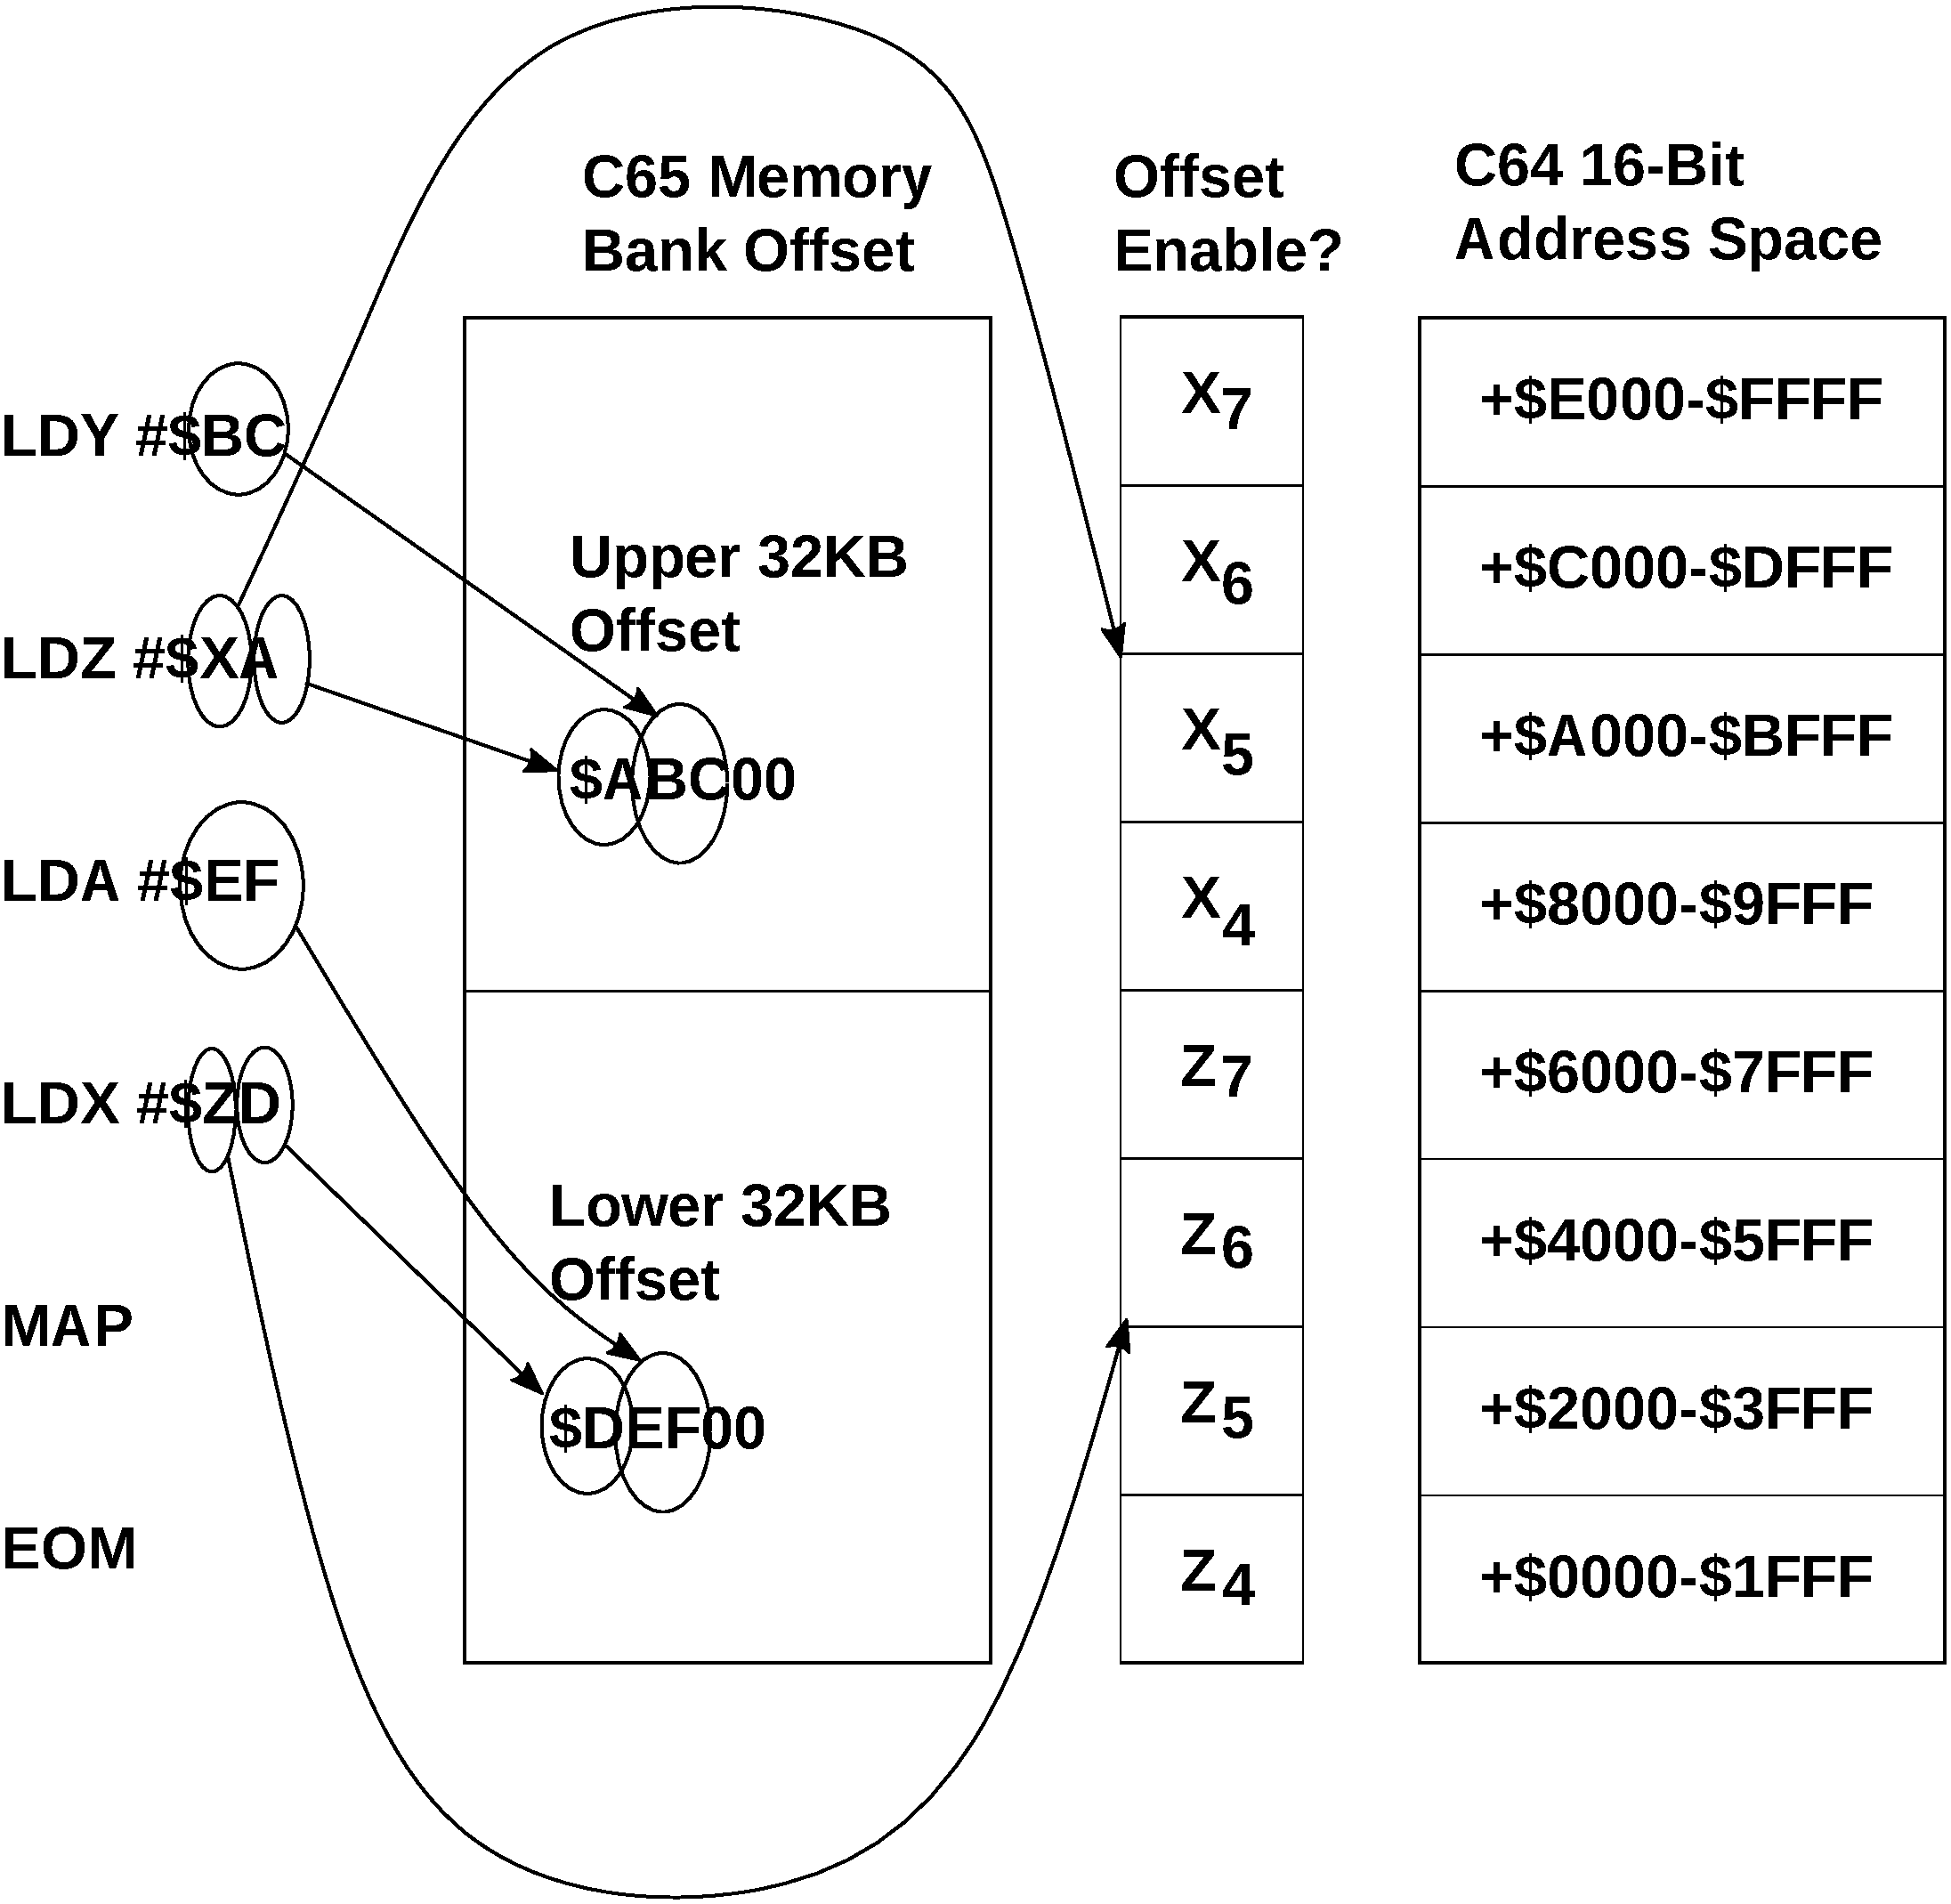
\includegraphics[width=0.75\textwidth]{images/illustrations/map-instruction-operation.pdf}\index{MAP}\index{Memory banking}
\end{center}

That is, the contents of the A register and the lower-nibble of the X register form a 12-bit value
that is multiplied by 256 to produce the offset used for any of the 8KB banks in the lower 32KB half of the 6502's 16-bit address
space.  The upper nibble of the X register is used as flags to indicate which of the four 8KB blocks in that 32KB half of the
6502 address space should have the offset added to their addresses to compute the actual address.

The Y and Z registers are used in a similar way to produce the offset for the upper 32KB half of the 6502 address space, and the
flags to indicate whether the offset is used for each of the four 8KB blocks in that half of the address space.

Note that the lower 8 bits of the offset cannot be set. That is, the offset will be a multiple of 256
bytes, unlike on some extended 6502 processors.  However, in practice this restriction is rarely
limiting.

To understand how this works in practice, the following example shows how this works with a concrete
example, showing the address ranges that would be visible in each of the 8KB slices of the 6502's
64KB address space:

\begin{center}
  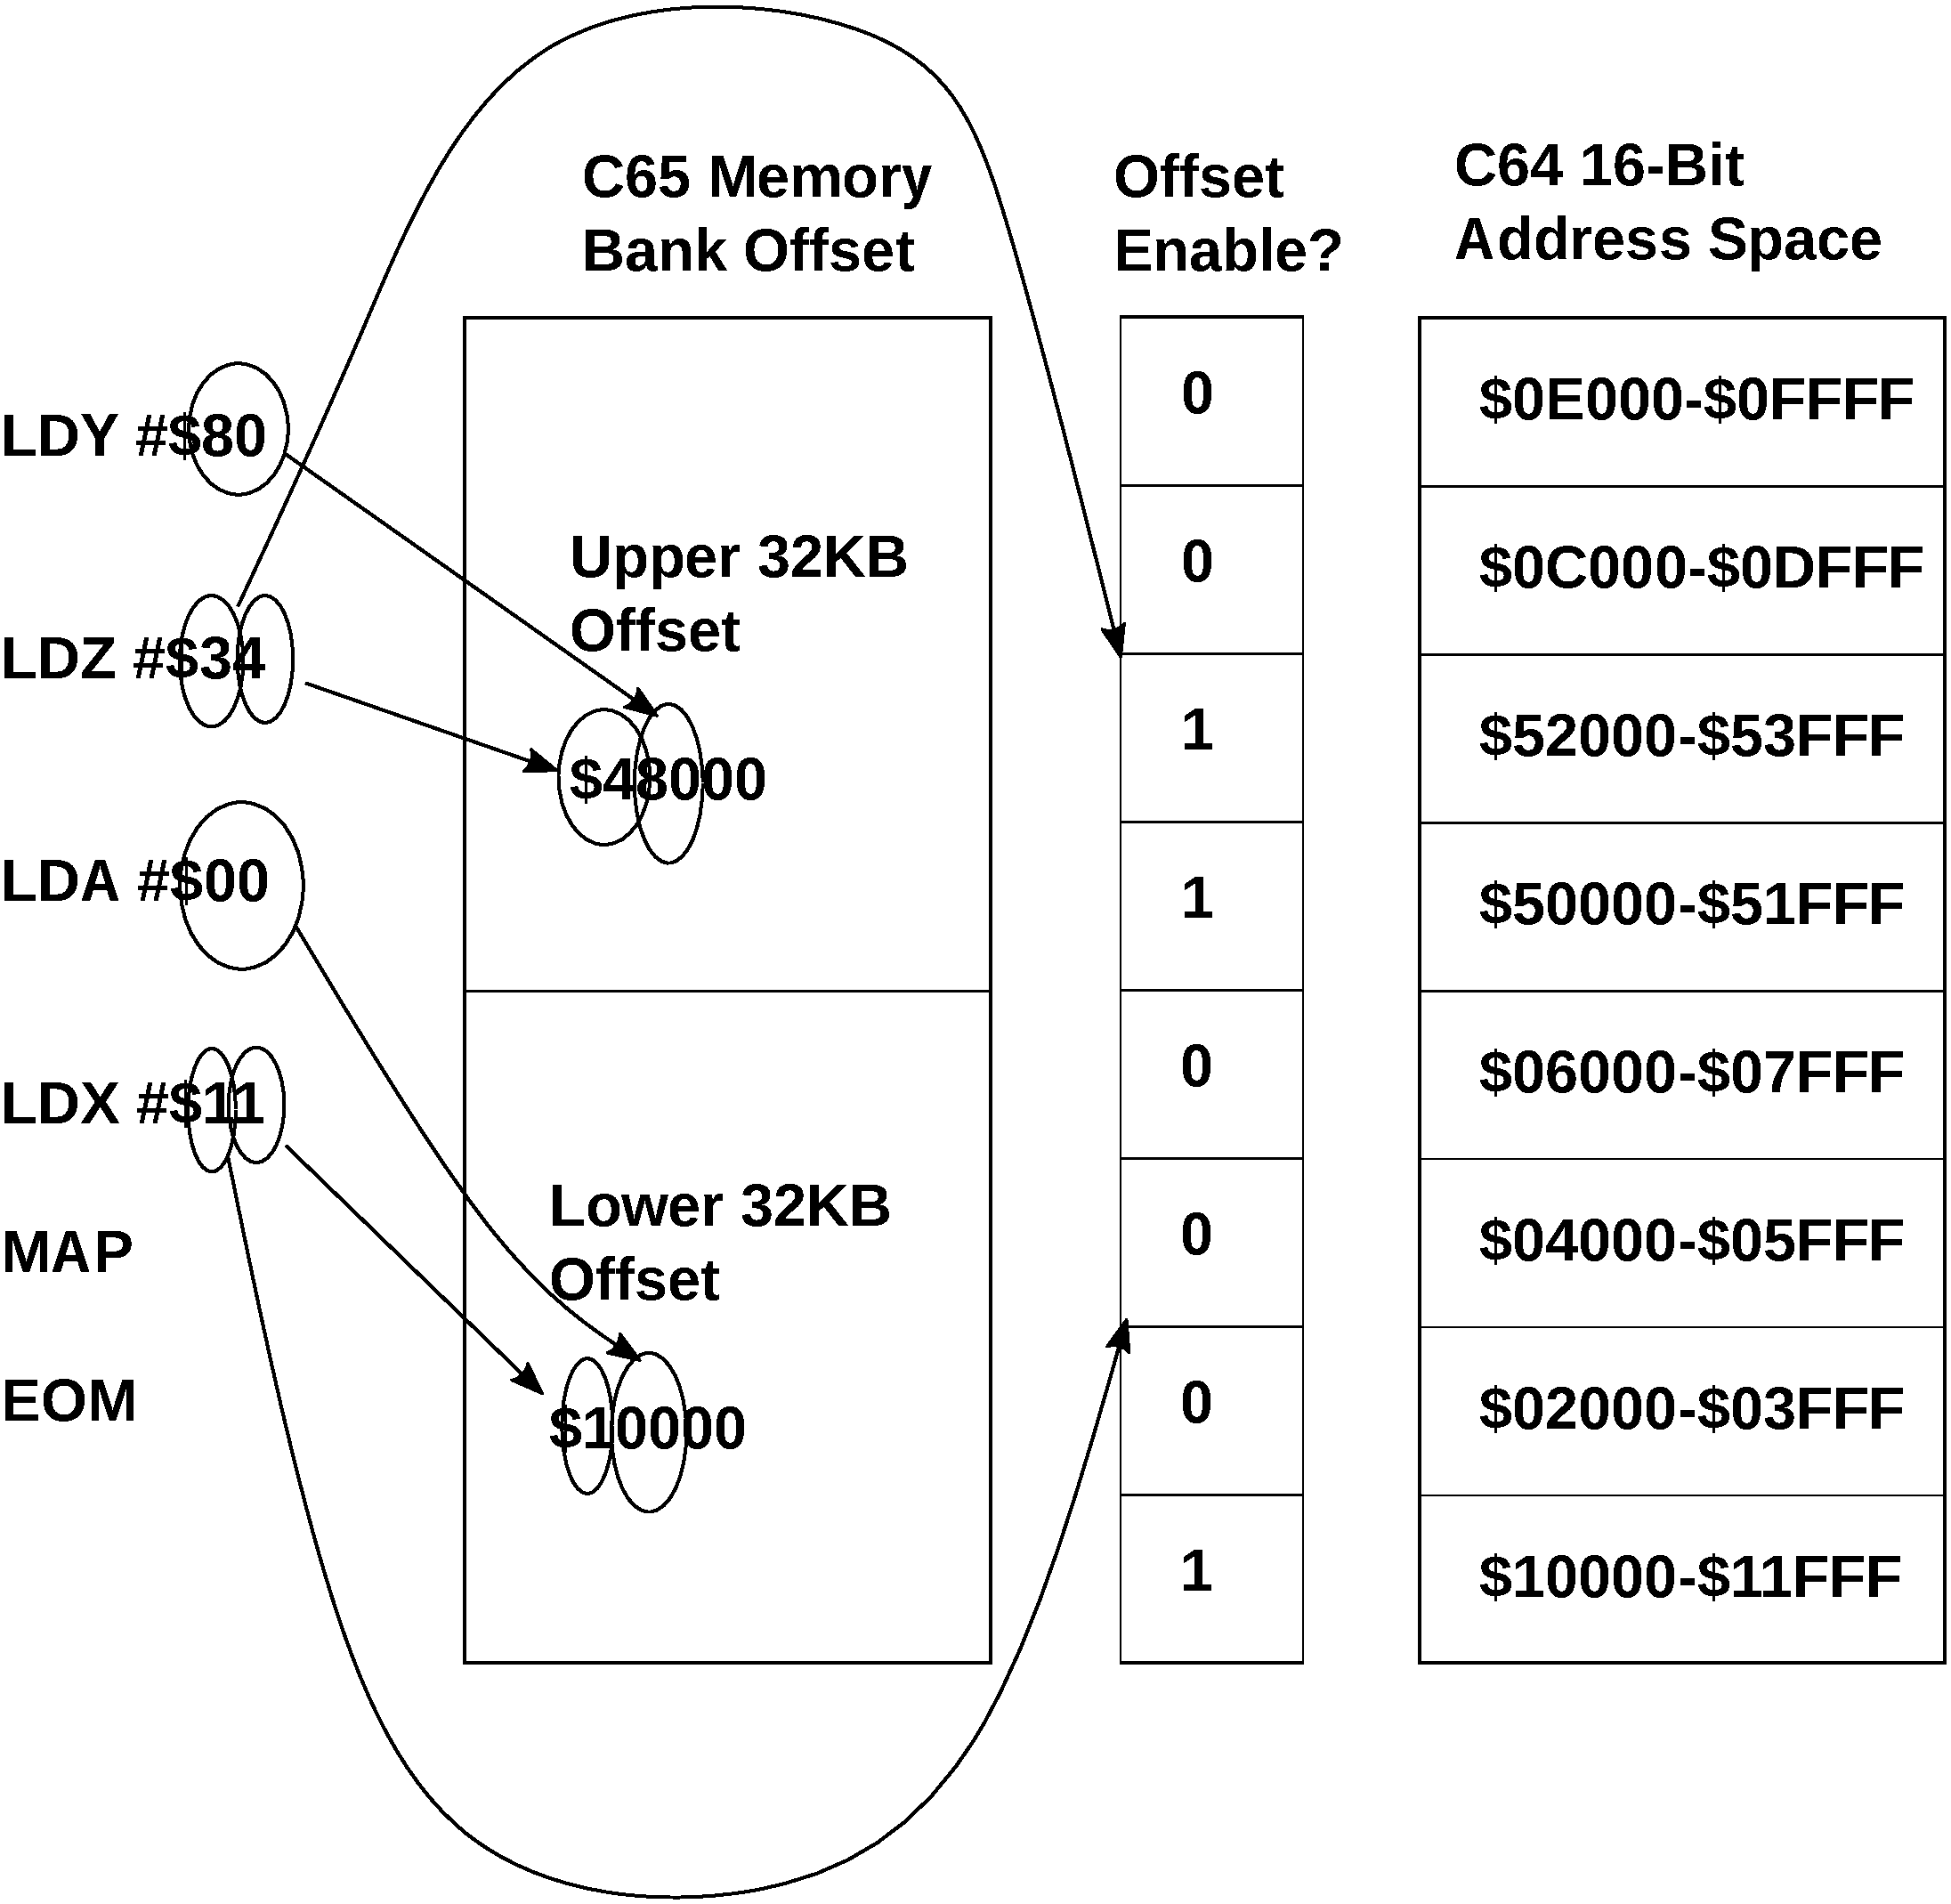
\includegraphics[width=0.75\textwidth]{images/illustrations/map-instruction-operation-example1.pdf}\index{MAP}\index{Memory banking}
\end{center}

Notice that the offsets for each of the two 32KB address ranges get added to the 6502 address.
This is why the offset of \$48000 for the upper 32KB generates an address of \$50000 at the 6502
address \$8000.

See also under ``Using the MAP instruction to access >1MB'' for further explanation.

\subsubsection{Direct Memory Access (DMA) Controller}

The C65's F018/F018A DMA controller allows for rapid filling, copying and swapping of the contents of memory
anywhere in the 1MB address space. Detailed information about the F018 DMA controller, and the MEGA65's
enhancements to this, refer to \bookvref{cha:dmagic}

\subsubsection{Flat Memory Access}

\subsection{Accessing memory beyond the 1MB point}
\label{sec:extended-memory}

The MEGA65 can support up to 256MB of memory. This is more than the 1MB address space of the CSG4510
on which it is based. There are several ways of performing this.

\subsubsection{Using the MAP instruction to access >1MB}

The full address space is available to the MAP instruction for legacy C65-style memory
mapping, although some care is required, as the MAP instruction must be called up to three times.
The reason for this is that the MAP instruction must be called to first select which mega-byte of
memory will be used for the lower and upper map regions, before it is again called in the normal
way to set the memory mapping.  Because between these two calls the memory mapping offset will be
a mix of the old and new addresses, all mapping should be first disabled via the MAP instruction.
This means that the code to re-map memory should live in the bottom 64KB of RAM or in one of the
ROM-bankable regions, so that it can remain visible during the mapping process.

Failure to handle this situation properly will result in the processor executing instructions
from somewhere unexpected half-way through the process, because the routine it is executing
to perform the mapping will suddenly no longer be mapped.

Because of the relative complexity of this process, and the other problems with the MAP instruction
as a means of memory access, we recommend that for accessing data outside of the current memory
map that you use either DMA or the flat-memory address features of the 45GS02 that are described below.
Indeed, access to the full address space via the MAP instruction is only provided for completeness.

As an other example of how the MAP instruction can be used to map an area of memory from
the expanded address space, the following program maps the Ethernet frame buffer from its natural location
at \$FFDE8000 to appear at \$6800.  To keep the example as simple as possible, we assume that the code
is running from in the bottom 64KB of RAM, and not in the region between \$6000 -- \$8000.

As the MAP instruction normally is only aware of the C65-style 20-bit addresses, the MEGA65 extension to the
instruction must be used to set the upper 8 bits of the 28-bit MEGA65 addresses, i.e., which mega-byte of address
space should be used for the address translation.  This is done by setting the X
register to \$0F when setting the mega-byte number for the lower-32KB of the C64-style 64KB address space.
This does not create any incompatibility with any sensible use of the MAP instruction on a C65, because this
value indicates that none of the four 8KB memory blocks will be re-mapped, but at the same time specifies that
the upper 4 bits of the address offset for re-mapped block is the non-zero value of \$F.  The mega-byte number
is then specified by setting the A register.

The same approach applies to the upper 32KB, but using the Z and Y
registers instead of the X and A registers.  However, in this case, we do not need to re-map the upper 32KB of
memory in this example, we will leave the Z and Y registers set to zero.  We must however set X and A to
set the mega-byte number for the lower-32KB to \$FF. Therefore A must have the value \$FF.  To set the lower 20-bits
of the address offset we use the MAP instruction a second time, this time using it in the normal C65 manner.
As we want to remap \$6800 to \$FFDE800, and have already dealt with the \$FFxxxxx offset via the mega-byte number,
we need only to apply the offset to make \$6800 point to \$DE800. \$DE800 minus \$6800 = \$D8000.  As the MAP instruction
operates with a mapping granularity of 256 bytes = \$100, we can drop the last two digits from \$D8000 to obtain the
MAP offset of \$D80. The lower 8-bits, \$80, must be loaded into the A register. The upper 4-bits, \$D, must be loaded into
the low-nibble of the X register.  As we wish to apply the mapping to only the fourth of the 8KB blocks that make up the
lower 32KB half of the C64 memory map, we must set the 4th bit of the upper nibble. That is, the upper nibble must be set
to \%1000, i.e., \$8.  Therefore the X register must be loaded with \$8D.  Thus we yield the complete example program:

\begin{screenoutput}
; Map Ethernet registers at $6000 - $7FFF

; Ethernet controller really lives $FFDE000 - $FFDEFFF, so select $FF megabyte section for MAP LO
LDA #$ff
LDX #$0f
LDY #$00
LDZ #$00
map

; now enable mapping of $DE000-$DFFFF at $6000
; MAPs are offset based, so we need to subtract $6000 from the target address
; $DE000 - $6000 = $D8000
LDA #$80
LDX #$8d
LDY #$00
LDZ #$00
map
EOM

; Ethernet buffer now visible at $6800 - $6FFF
\end{screenoutput}

Note that the EOM (End Of Mapping) instruction (which is the same as NOP on a 6502, i.e., opcode \$EA) was only supplied after the last MAP instruction, to make sure that no interrupts could occur while
the memory map contained mixed values with the mega-byte number set, but the lower-bits of the mapping address had not been
updated.

No example in BASIC for the MAP instruction is possible, because the MAP is an machine code instruction of the 4510 / 45GS02 processors.

\subsubsection{Flat-Memory Access}

The 45GS02 makes it easy to read or write a byte from anywhere in memory by allowing the Zero-Page Indirect
addressing mode to use a 32-bit pointer instead of the normal 16-bit pointer.  This is accomplished by
using the Z-indexed Zero-Page Indirect Addressing Mode for the access, and having the instruction directly
preceded by a NOP instruction (opcode \$EA).  For example:

\begin{screenoutput}
NOP
LDA ($45),Z
\end{screenoutput}

If you are using the ACME assembler, or another assembler that supports the 45GS02 extensions, you can instead use square-brackets
to indicate that you are performing a flat-memory operation. Such assemblers will insert the \$EA prefix automatically for you. For example:

\begin{screenoutput}
LDA [$45],Z
\end{screenoutput}

Regardless which tool you are using, this example would read the four bytes of Zero-Page memory at \$45 -- \$48 to form a 32-bit memory address, and add the value of the
Z register to this to form the actual address that will be read from.  The byte order in the address is the same as
the 6502, i.e., the right-most (least significant) byte of the address will be read from the first address (\$45 in this case),
and so on, until the left-most (most significant) byte will be read from \$48.  For example, to read from memory location
\$12345678, the contents of memory beginning at \$45 should be 78 56 34 12.

This method is much more efficient and also simpler than either using the MAP instruction or the DMA controller for single memory accesses,
and is what we generally recommend.  The DMA controller can be used for moving/filler larger regions of memory.
We recommend the MAP instruction only be used for banking code, or in rare situations where extensive access to a small region of
memory is required, and the extra cycles of reading the 32-bit addresses is problematic.

\subsection{Virtual 32-bit Register}

The 45GS02 allows the use of its four general purpose registers, A, X, Y and Z (A is LSB, Z is MSB) as a single virtual 32-bit register, 
also called the {\em Q pseudo register}.
This can greatly simplify and speed up many common operations, and help avoid many common programming errors.
For example, adding two 16-bit or 32-bit values can now be easily accomplished with something like:

\begin{screenoutput}
  ; Clear carry before performing addition, as normal
  CLC
  ; Prefix an instruction with two NEG instructions to select virtual 32-bit register mode
  NEG
  NEG
  LDA $1234  ; Load the contents of $1234-$1237 into A,X,Y and Z respectively
  ; And again, for the addition
  NEG
  NEG
  ADC $1238  ; Add the contents of $1238-$123B
  ; The result of the addition is now in A, X, Y and Z.
  ; And can be written out in whole or part

  ; To write it all out, again, we need the NEG + NEG prefix
  NEG
  NEG
  STA $123C ; Write the whole out to $123C-$123F

  ; Or to write out the bottom bytes, we can just write the contents of A and X as normal
  STA $1240
  STX $1241
\end{screenoutput}

This approach works with the LDA, STA, ADC, SBC, CMP, EOR, AND, BIT, ORA, ASL, ASR, LSR, ROL, ROR, INC and DEC instructions.
If you are using ACME or another 45GS02 aware assembler, you can instead use the new \stw{LDQ}, \stw{STQ}, \stw{ADCQ},
\stw{SBCQ}, \stw{CPQ}, \stw{EORQ}, \stw{ANDQ}, \stw{BITQ}, \stw{ORQ}, \stw{ASLQ}, \stw{ASRQ}, \stw{LSRQ}, \stw{ROLQ}, \stw{RORQ}, \stw{INQ} and \stw{DEQ}
mnemonics.\index{LDQ}\index{STQ}\index{ADCQ}\index{SBCQ}\index{CPQ}\index{EORQ}\index{ANDQ}\index{BITQ}\index{ORQ}\index{ASLQ}\index{ASRQ}\index{LSRQ}\index{ROLQ}\index{RORQ}\index{INQ}\index{DEQ} The previous example would thus become:

\begin{screenoutput}
  ; Clear carry before performing addition, as normal
  CLC
  LDQ  $1234  ; Load the contents of $1234-$1237 into A,X,Y and Z respectively
  ADCQ $1238  ; Add the contents of $1238-$123B
  ; The result of the addition is now in A, X, Y and Z.
  ; And can be written out in whole or part

  ; To write it all out, again, we need the NEG + NEG prefix
  STQ $123C ; Write the whole out to $123C-$123F

  ; Or to write out the bottom bytes, we can just write the contents of A and X as normal
  STA $1240
  STX $1241
\end{screenoutput}

The virtual 32-bit addressing mode works with any addressing mode.
However, indexed addressing modes, where X, Y or Z are added to the address should
be used with care, because these registers may in fact be holding part of a 32-bit value.

The exception is the Zero-Page Indirect Z-Indexed addressing mode: In this case the Z register is NOT added to the target address
(with the exception of the LDQ opcode), unlike would normally be the case. This is to allow the virtual 32-bit register to be able
to be used with flat-memory access with the combined prefix of \stw{NEG NEG NOP},  before the instruction to allow accessing a
32-bit value anywhere in memory in a single instruction.

Note that the virtual 32-bit register cannot be used in immediate mode, e.g., to load a constant into the four general
purpose registers, or to add or subtract a constant value.  This is to avoid problems with variable length instructions.

For LDQ and STQ, it would save at most one byte
compared to LDA \#\$nn ... LDZ \#\$nn, and would be no faster.  In fact, for many common
values, such as \#\$00000000, there are short-cuts, such as:

\begin{screenoutput}
LDA #$00
TAX
TAY
TAZ
\end{screenoutput}

If you need to add or subtract a 32-bit immediate value, this may require you to re-order the arguments, or perform other
minor gymnastics.  For example, to compute the sum of the contents of memory and an immediate value, you can load the A, X, Y
and Z registers with the immediate value, and then use \stw{ADCQ} with the memory address, e.g.:

\begin{screenoutput}
  ; Get the immediate value #$12345678 into Q
  LDA #$78
  LDX #$56
  LDY #$34
  LDZ #$12
  ; Add the contents of memory locations $1234-$1237
  NEG
  NEG
  ADC $1234
  ; Store the result back in $1234-$1237
  NEG
  NEG
  STA $1234
\end{screenoutput}

Again, if you are using the ACME or another 45GS02-aware assembler, this can be more compactly and
clearly written as follows. But note that in both cases the same byte-sequence of machine code is
produced, and the program will take the same number of cycles to execute.

\begin{screenoutput}
  ; Get the immediate value #$12345678 into Q
  LDA #$78
  LDX #$56
  LDY #$34
  LDZ #$12
  ; Add the contents of memory locations $1234-$1237
  ADCQ $1234
  ; Store the result back in $1234-$1237
  STQ $1234
\end{screenoutput}

\section{C64 CPU Memory Mapped Registers}

\input{regtable_CPU.C64}

\section{New CPU Memory Mapped Registers}

\input{regtable_CPU.MEGA65}

\section{MEGA65 CPU Maths Acceleration Registers}

Every MEGA65 contains a combined 32-bit hardware multiplier and divider.
This device takes two 32-bit inputs, {\bf MULTINA} and {\bf MULTINB}, and simultaneously calculates:

\begin{itemize}
\item the 64-bit product {\bf MULTOUT} of {\bf MULTINA} and {\bf MULTINB}
\item the 32-bit whole part {\bf DIVOUT}(4-7) of {\bf MULTINA} divided by {\bf MULTINB}
\item the 32-bit fractional part {\bf DIVOUT}(0-3) of {\bf MULTINA} divided by {\bf MULTINB}
\end{itemize}

It is always updating the outputs based on the inputs, so there is no need to take special action when changing the inputs.
The multiplier takes 1 cycle to calculate, and the updated result will thus be available immediately (a {\bf MULBUSY} bit is
defined, but currently it won't be set at all). The hardware divider, however, can take upto 20 cycles depending on the
particular inputs. The programmer should check the {\bf DIVBUSY} bit if the divider is still calculating:

\begin{screenoutput}
loop:   BIT $D70F   ; transfer DIVBUSY bit into N flag
        BMI loop    ; as long as it is set, we need to wait
\end{screenoutput}

The MEGA65 is planned to also include a programmable math unit, which helps to accelerate the calculation of fixed-point formulae.
This is presently disabled and will be further documented if and when it becomes available (addresses \$D780 - \$D7E3).

\input{regtable_MATH.MEGA65}

\section{MEGA65 Hypervisor Mode}
\label{sec:hypervisor-mode}

\subsection{Reset}

On power-up or reset, the MEGA65 starts up in hypervisor mode, and expects to find a program in the
16KB hypervisor memory, and begins executing instructions at address \$8100.  Normally a JMP instruction
will be located at this address, that will jump into a reset routine. That is, the 45GS02
does not use the normal 6502 reset vector. It's function is emulated by the Hyppo hypervisor program,
which fetches the address from the 6502 reset vector in the loaded client operating system when
exiting hypervisor mode.

The hypervisor memory is automatically mapped on reset to \$8000 - \$BFFF.  This special memory is not
able to mapped or in anyway accessed, except when in hypervisor mode. It can, however, always be accessed from the serial monitor/debugger
interface via its 28-bit address, \$FFF8000 -- \$FFFBFFF.  This is to protect it from accidental or malicious access from a guest operating system.

\subsection{Entering / Exiting Hypervisor Mode}

Entering the Hypervisor occurs whenever any of the following events occurs:

\begin{itemize}
\item{\bf Power-on} When the MEGA65 is first powered on.
\item{\bf Reset} If the reset line is lowered, or a watch-dog triggered reset occurs.
\item{\bf SYSCALL register accessed} The registers \$D640 - \$D67F in the MEGA65 I/O context trigger SYSCALLs when accessed.
  This is intended to be the mechanism by which a client operating system or process requests the attention of the hypervisor or operating system.
\item{\bf Page Fault} On MEGA65s that feature virtual memory, a page fault will cause a trap to hypervisor mode.
\item{\bf Certain keyboard events} Pressing \widekey{RESTORE} for >0.5 seconds, or the \specialkey{ALT} and
\specialkey{TAB} key combination traps to the hypervisor.  Typically the first is used to launch the Freeze Menu an the second to toggle the display of debug interface.
\item{\bf Accessing virtualised I/O devices} For example, if the F011 (internal 3.5'' disk drive controller) has been virtualised, then attempting to read or write sectors using this device will cause traps to the hypervisor.
  \item{\bf Executing an instruction that would lock up the CPU} A number of undocumented opcodes on the 6502 will cause the CPU to lockup.  On the MEGA65, instead of locking up, the computer will trap to the hypervisor.  This could be used to implement alternative instruction behaviours, or simply to tell the user that something bad has happened.
  \item{\bf Certain special events} Some devices can generate hypervisor-level interrupts. These are implemented as traps to the hypervisor.
\end{itemize}

The 45GS02 handles all of these in a similar manner internally:

\begin{enumerate}
\item The SYSCALL or trap address is calculated, based on the event.
\item The contents of all CPU registers are saved into the virtualisation control registers.
\item The hypervisor mode memory layout is activated, the CPU decimal flag and special purpose registers are all set to appropriate values.  The contents of the A,X,Y and Z and most other CPU flags are preserved, so that they can be accessed from the Hypervisor's SYSCALL/trap handler routine, without having to load them, thus saving a few cycles for each call.
\item The hypervisor-mode flag is asserted, and the program counter (PC) register is set to the computed address.
\end{enumerate}

All of the above happens in one CPU cycle, i.e., in 25 nano-seconds.
Returning from a SYSCALL or trap consists simply of writing to \$D67F, which
requires 125 nano-seconds, for a total overhead of 150 nano-seconds.
This gives the MEGA65 SYSCALL performance rivalling -- even beating
-- even the fastest modern computers, where the system call latency is
typically hundreds to tens of thousands of cycles \cite{soares2010flexsc}.

\subsection{Hypervisor Memory Layout}

The hypervisor memory is 16KB in size.  The first 512 bytes are
reserved for SYSCALL and system trap entry
points, with four bytes for each.  For example, the reset entry point is
at \$8100 - \$8100 + 3 = \$8100 - \$8103.
This allows 4 bytes for an instruction, typically a JMP instruction,
followed by a NOP to pad it to 4 bytes.

The full list of SYSCALLs and traps is:

\begin{longtable}{|L{1.2cm}|L{1.1cm}|C{2cm}|L{6cm}|}
\hline
{\bf{HEX}} & {\bf{DEC}} & {\bf{Name}} & {\bf{Description}} \\
\hline
\endfirsthead
\multicolumn{3}{l@{}}{\ldots continued}\\
\hline
{\bf{HEX}} & {\bf{DEC}} & {\bf{Name}} & {\bf{Description}} \\
\hline
\endhead
\multicolumn{3}{l@{}}{continued \ldots}\\
\endfoot
\hline
\endlastfoot
\small  8000 & \small 32768 & SYSCALL00 & SYSCALL 0 entry point \\
\hline
\small  8004 & \small 32772 & SYSCALL01 & SYSCALL 1 entry point \\
\hline
\small  8008 & \small 32776 & SYSCALL02 & SYSCALL 2 entry point \\
\hline
\small  800C & \small 32780 & SYSCALL03 & SYSCALL 3 entry point \\
\hline
\small  8010 & \small 32784 & SYSCALL04 & SYSCALL 4 entry point \\
\hline
\small  8014 & \small 32788 & SYSCALL05 & SYSCALL 5 entry point \\
\hline
\small  8018 & \small 32792 & SYSCALL06 & SYSCALL 6 entry point \\
\hline
\small  801C & \small 32796 & SYSCALL07 & SYSCALL 7 entry point \\
\hline
\small  8020 & \small 32800 & SYSCALL08 & SYSCALL 8 entry point \\
\hline
\small  8024 & \small 32804 & SYSCALL09 & SYSCALL 9 entry point \\
\hline
\small  8028 & \small 32808 & SYSCALL0A & SYSCALL 10 entry point \\
\hline
\small  802C & \small 32812 & SYSCALL0B & SYSCALL 11 entry point \\
\hline
\small  8030 & \small 32816 & SYSCALL0C & SYSCALL 12 entry point \\
\hline
\small  8034 & \small 32820 & SYSCALL0D & SYSCALL 13 entry point \\
\hline
\small  8038 & \small 32824 & SYSCALL0E & SYSCALL 14 entry point \\
\hline
\small  803C & \small 32828 & SYSCALL0F & SYSCALL 15 entry point \\
\hline
\small  8040 & \small 32832 & SYSCALL10 & SYSCALL 16 entry point \\
\hline
\small  8044 & \small 32836 & SECURENTR & Enter secure container trap entry point \\
\hline
\small  8048 & \small 32840 & SECUREXIT & Leave secure container trap entry point. \\
\hline
\small  804C & \small 32844 & SYSCALL13 & SYSCALL 19 entry point \\
\hline
\small  8050 & \small 32848 & SYSCALL14 & SYSCALL 20 entry point \\
\hline
\small  8054 & \small 32852 & SYSCALL15 & SYSCALL 21 entry point \\
\hline
\small  8058 & \small 32856 & SYSCALL16 & SYSCALL 22 entry point \\
\hline
\small  805C & \small 32860 & SYSCALL17 & SYSCALL 23 entry point \\
\hline
\small  8060 & \small 32864 & SYSCALL18 & SYSCALL 24 entry point \\
\hline
\small  8064 & \small 32868 & SYSCALL19 & SYSCALL 25 entry point \\
\hline
\small  8068 & \small 32872 & SYSCALL1A & SYSCALL 26 entry point \\
\hline
\small  806C & \small 32876 & SYSCALL1B & SYSCALL 27 entry point \\
\hline
\small  8070 & \small 32880 & SYSCALL1C & SYSCALL 28 entry point \\
\hline
\small  8074 & \small 32884 & SYSCALL1D & SYSCALL 29 entry point \\
\hline
\small  8078 & \small 32888 & SYSCALL1E & SYSCALL 30 entry point \\
\hline
\small  807C & \small 32892 & SYSCALL1F & SYSCALL 31 entry point \\
\hline
\small  8080 & \small 32896 & SYSCALL20 & SYSCALL 32 entry point \\
\hline
\small  8084 & \small 32900 & SYSCALL21 & SYSCALL 33 entry point \\
\hline
\small  8088 & \small 32904 & SYSCALL22 & SYSCALL 34 entry point \\
\hline
\small  808C & \small 32908 & SYSCALL23 & SYSCALL 35 entry point \\
\hline
\small  8090 & \small 32912 & SYSCALL24 & SYSCALL 36 entry point \\
\hline
\small  8094 & \small 32916 & SYSCALL25 & SYSCALL 37 entry point \\
\hline
\small  8098 & \small 32920 & SYSCALL26 & SYSCALL 38 entry point \\
\hline
\small  809C & \small 32924 & SYSCALL27 & SYSCALL 39 entry point \\
\hline
\small  80A0 & \small 32928 & SYSCALL28 & SYSCALL 40 entry point \\
\hline
\small  80A4 & \small 32932 & SYSCALL29 & SYSCALL 41 entry point \\
\hline
\small  80A8 & \small 32936 & SYSCALL2A & SYSCALL 42 entry point \\
\hline
\small  80AC & \small 32940 & SYSCALL2B & SYSCALL 43 entry point \\
\hline
\small  80B0 & \small 32944 & SYSCALL2C & SYSCALL 44 entry point \\
\hline
\small  80B4 & \small 32948 & SYSCALL2D & SYSCALL 45 entry point \\
\hline
\small  80B8 & \small 32952 & SYSCALL2E & SYSCALL 46 entry point \\
\hline
\small  80BC & \small 32956 & SYSCALL2F & SYSCALL 47 entry point \\
\hline
\small  80C0 & \small 32960 & SYSCALL30 & SYSCALL 48 entry point \\
\hline
\small  80C4 & \small 32964 & SYSCALL31 & SYSCALL 49 entry point \\
\hline
\small  80C8 & \small 32968 & SYSCALL32 & SYSCALL 50 entry point \\
\hline
\small  80CC & \small 32972 & SYSCALL33 & SYSCALL 51 entry point \\
\hline
\small  80D0 & \small 32976 & SYSCALL34 & SYSCALL 52 entry point \\
\hline
\small  80D4 & \small 32980 & SYSCALL35 & SYSCALL 53 entry point \\
\hline
\small  80D8 & \small 32984 & SYSCALL36 & SYSCALL 54 entry point \\
\hline
\small  80DC & \small 32988 & SYSCALL37 & SYSCALL 55 entry point \\
\hline
\small  80E0 & \small 32992 & SYSCALL38 & SYSCALL 56 entry point \\
\hline
\small  80E4 & \small 32996 & SYSCALL39 & SYSCALL 57 entry point \\
\hline
\small  80E8 & \small 33000 & SYSCALL3A & SYSCALL 58 entry point \\
\hline
\small  80EC & \small 33004 & SYSCALL3B & SYSCALL 59 entry point \\
\hline
\small  80F0 & \small 33008 & SYSCALL3C & SYSCALL 60 entry point \\
\hline
\small  80F4 & \small 33012 & SYSCALL3D & SYSCALL 61 entry point \\
\hline
\small  80F8 & \small 33016 & SYSCALL3E & SYSCALL 62 entry point \\
\hline
\small  80FC & \small 33020 & SYSCALL3F & SYSCALL 63 entry point \\
\hline
\small  8100 & \small 33024 & RESET & Power-on/reset entry point \\
\hline
\small  8104 & \small 33028 & PAGFAULT & Page fault entry point (not currently used) \\
\hline
\small  8108 & \small 33032 & RESTORKEY & Restore-key long press trap entry point \\
\hline
\small  810C & \small 33036 & ALTTABKEY & ALT+TAB trap entry point \\
\hline
\small  8110 & \small 33040 & VF011RD & F011 virtualised disk read trap entry point \\
\hline
\small  8114 & \small 33044 & VF011WR & F011 virtualised disk write trap entry point \\
\hline
\small  8118 & \small 33048 & BREAKPT & CPU break-point encountered \\
\hline
\small  811C -- 81FB & \small 33048 -- 33275 & RESERVED & Reserved traps point entry \\
\hline
\small  81FC & \small 33276 & CPUKIL & KIL instruction in 6502-mode trap entry point \\
\hline
\end{longtable}

The remainder of the 16KB hypervisor memory is available for use by the programmer, but
will typically use the last 512 bytes for the stack and zero-page, giving an overall memory map as follows:

\begin{longtable}{|L{1.2cm}|L{1.1cm}|L{8cm}|}
\hline
{\bf{HEX}} & {\bf{DEC}} & {\bf{Description}} \\
\hline
\endfirsthead
\multicolumn{3}{l@{}}{\ldots continued}\\
\hline
{\bf{HEX}} & {\bf{DEC}} & {\bf{Description}} \\
\hline
\endhead
\multicolumn{3}{l@{}}{continued \ldots}\\
\endfoot
\hline
\endlastfoot
\small  8000 -- 81FF & \small 32768 -- 33279 & SYSCALL and trap entry points \\
\hline
\small  8200 -- BDFF & \small 33280 -- 48639 & Available for hypervisor or operating system program \\
\hline
\small  8E00 -- BEFF & \small 48640 -- 48895 & Processor stack for hypervisor or operating system \\
\hline
\small  8F00 -- BFFF & \small 48896 -- 49151 & Processor zero-page storage for hypervisor or operating system \\
\hline
\end{longtable}

The stack is used for holding the return address of function calls.  The zero-page storage is typically used for holding
variables and other short-term storage, as is customary on the 6502.

\subsection{Hypervisor Virtualisation Control Registers}

\input{regtable_HCPU.MEGA65}

\subsection{Programming for Hypervisor Mode}

The easiest way to write a program for Hypervisor Mode on the MEGA65 is to use KickC, which is a special version of C
made for writing programs for 6502-class processors.  The following example programs are from KickC's supplied examples.
KickC produces very efficient code, and directly supports the MEGA65's
hypervisor mode quite easily through the use of a linker definition file with the following contents:

\begin{screenoutput}
.file [name="%O.bin", type="bin", segments="XMega65Bin"]
.segmentdef XMega65Bin [segments="Syscall, Code, Data, Stack, Zeropage"]
.segmentdef Syscall [start=$8000, max=$81ff]
.segmentdef Code [start=$8200, min=$8200, max=$bdff]
.segmentdef Data [startAfter="Code", min=$8200, max=$bdff]
.segmentdef Stack [min=$be00, max=$beff, fill]
.segmentdef Zeropage [min=$bf00, max=$bfff, fill]
\end{screenoutput}

This file instructs KickC's assembler to create a 16KB file with the 512 byte SYSCALL/trap entry point region at the start,
followed by code and data areas, and then the stack and zero-page areas. It enforces the size and location of these fields, and
will give an error during compilation if anything is too big to fit.

With this file in place, you can then create a KickC source file that provides data structures for the SYSCALL/trap table, e.g.:

\begin{screenoutput}
// XMega65 KERNAL Development Template
// Each function of the KERNAL is a no-args function
// The functions are placed in the SYSCALLS table surrounded by JMP and NOP

import "string"

// Use a linker definition file (put the previous listing into that file)
#pragma link("mega65hyper.ld")

// Some definitions of addresses and special values that this program uses
const char* RASTER = 0xd012;
const char* VIC_MEMORY = 0xd018;
const char* SCREEN = 0x0400;
const char* BGCOL = 0xd021;
const char* COLS = 0xd800;
const char BLACK = 0;
const char WHITE = 1;

// Some text to display
char[] MESSAGE = "hello world!";
\end{screenoutput}

\begin{screenoutput}
void main() {
    // Initialise screen memory, and select correct font
    *VIC_MEMORY = 0x14;
    // Fill the screen with spaces
    memset(SCREEN, ' ', 40*25);
    // Set the colour of every character on the screen to white
    memset(COLS, WHITE, 40*25);
    // Print the "hello world!" message
    char* sc = SCREEN+40;  // Display it one line down on the screen
    char* msg = MESSAGE; // The massage to display
    // A simple copy routine to copy the string
    while(*msg) {
        *sc++ = *msg++;
    }
    // Loop forever showing two white lines as raster bars
    while(true) {
        if(*RASTER==54 || *RASTER==66) {
            *BGCOL = WHITE;
        } else {
            *BGCOL = BLACK;
        }
    }
}

// Here are a couple sample SYSCALL handlers that just display a character on the screen
void syscall1() {
    *(SCREEN+79) = '>';
}

void syscall2() {
    *(SCREEN+78) = '<';
}

// Now we select the SYSCALL segment to hold the SYSCALL/trap entry point table.
#pragma data_seg(Syscall)

// The structure of each entry point is JMP <handler address> + NOP.
// We have a char (xjmp) to hold the opcode for the JMP instruction,
// and then put the address of the SYSCALL/trap handler in the next
// two points as a pointer, and end with the NOP instruction opcode.
\end{screenoutput}

\begin{screenoutput}
struct SysCall {
    char xjmp;         // Holds $4C, the JMP $nnnn opcode
    void()* syscall;   // Holds handler address, will be the target of the JMP
    char xnop;         // Holds $EA, the NOP opcode
};

// To save writing 0x4C and 0xEA all the time, we define them as constants
const char JMP = 0x4c;
const char NOP = 0xea;

// Now we can have a nice table of up to 64 SYSCALL handlers expressed
// in a fairly readable and easy format.
// Each line is an instance of the struct SysCall from above, with the JMP
// opcode value, the address of the handler routine and the NOP opcode value.
export struct SysCall[] SYSCALLS = {
    { JMP, &syscall1, NOP },
    { JMP, &syscall2, NOP }
    };

// In this example we had only two SYSCALLs defined, so rather than having
// another 62 lines, we can just ask KickC to make the TRAP table begin
// at the next multiple of $100, i.e., at $8100.
export align(0x100) struct SysCall[] SYSCALL\_RESET = {
    { JMP, &main, NOP }
};
\end{screenoutput}

If you save the first listing into a file called mega65hyper.ld, and the second
into a file called mega65hyper.kc, you can then compile them using KickC with
a command like:

\begin{screenoutput}
  kickc -a mega65hyper
\end{screenoutput}

It will then produce a file called mega65hyper.bin, which you can then try out
on your MEGA65, or run in the XMega65 emulator with a command like:

\begin{screenoutput}
  xmega65 -kickup mega65hyper.bin
\end{screenoutput}

  \chapter{45GS02 \& 6502 Instruction Sets}

The 45GS02 CPU is able to operate in native mode, where it
is compatible with the CSG 4510, and in 6502 compatibility mode,
where 6502 undocumented instructions, also known as illegal
instructions, are supported for compatibility.

When in 4510 compatibility mode, the 45GS02 also supports a number
of extensions through {\em compound instructions}. These work be prefixing
the desired instruction's opcode with one or more {\em prefix bytes}, which
represent sequences of instructions that should not normally occur.  For example,
two \stw{NEG} instructions in a row acts as a prefix to tell the 45GS02 that the
following instruction will operate on 32 bits of data, instead of the usual 8 bits
of data.  This means that a 45GS02 instruction stream can be readily decoded or disassembled,
without needing to set special instruction length flags, as is the case with the 65816
family of microprocessors. The trade-off is increased execution time, as the 45GS02 must
skip over the prefix-bytes.

The remainder of this chapter introduces the addressing modes, instructions, opcodes and
instruction timing data of the 45GS02, beginning with 6502 compatibility mode, before
moving on to 4510 compatibility mode, and the 45GS02 extensions.

\section{Addressing Modes}

The 45GS02 supports 36 different addressing modes, which are explained below.
Many of these are very similar to one another, being variations of the normal 6502
or 65CE02 addressing modes, except that they accept either
32-bit pointers, operate on 32-bits of data, or both.

\subsection{Implied}

In this mode, there are no operands, as the precise function of the instruction is
implied by the instruction itself.  For example, the \screentext{INX} instruction increments
the X Register.

\subsection{Accumulator}

In this mode, the Accumulator is the operand. This is typically used to shift,
rotate or modify the value of the Accumulator Register in some way.  For example,
\screentext{INC A} increments the value in the Accumulator Register.

\subsection{Q Pseudo Register}

In this mode, the Q Pseudo Register is the operand. This is typically used to shift,
rotate or modify the value of the Q Pseudo Register in some way.  For example,
\screentext{ASL Q} shifts the value in the Q Pseudo Register left one bit.

Remember that the Q Pseudo Register is simply the A, X, Y and Z registers acting together
as a pseudo 32-bit register, where A contains the least significant bits, and Z the
most significant bits.  There are some cases where using a Q mode instruction can be
helpful for operating on the four true registers.

\subsection{Immediate Mode}

In this mode, the argument to the instruction is a value that is used directly.
This is indicated by proceeding the value with a \# character. Most assemblers allow
values to be entered in decimal, or in hexadecimal by preceding the value with a \$ sign,
in binary, by preceding the value with a \% sign.  For example, to set the Accumulator
Register to the value 5, you could use the following:

\begin{tcolorbox}[colback=black,coltext=white]
\verbatimfont{\codefont}
\begin{verbatim}
LDA #5
\end{verbatim}
\end{tcolorbox}

The immediate argument is encoded as a single byte following the instruction.  For the above
case, the instruction stream would contain \$A9, the opcode for LDA immediate mode, followed
by \$05, the immediate operand.

\subsection{Immediate Word Mode}

In this mode, the argument is a 16-bit value that is used directly. There is only one instruction
which uses this addressing mode, \screentext{PHW}.  For example, to push the word \$1234
onto the stack, you could use:

\begin{tcolorbox}[colback=black,coltext=white]
\verbatimfont{\codefont}
\begin{verbatim}
PHW #$1234
\end{verbatim}
\end{tcolorbox}

The low byte of the immediate value follows the opcode of the instruction.  The high byte of the
immediate value then follows that.  For the above example, the instruction stream would thus
be \$F4 \$34 \$12.

\subsection{Base Page (Zero-Page) Mode}

In this mode, the argument is an 8-bit address.  The upper 8-bits of the address are taken from
the Base Page Register.  On 6502 processors, there is no Base Page Register, and instead, the
upper 8-bits are always set to zero -- hence the name of this mode on the 6502: Zero-Page. On
the 45GS02, it is possible to move this ``Zero-Page'' to any page in the processor's 64KB view
of memory by setting the Base Page Register using the \screentext{TAB} instruction. Base Page
Mode allows faster access to a 256 region of memory, and uses less instruction bytes to do so.

The argument is encoded as a single byte that immediately follows the instruction opcode. For
example, \screentext{LDA \$12} would read the value stored in location \$12 in the Base Page,
and put it into the Accumulator Register.  The instruction byte stream for this would be
\$85 \$12.

\subsection{Base Page (Zero-Page) Quad Mode}

In this mode, the argument is an 8-bit address.  The upper 8-bits of the address are taken from
the Base Page Register.  On 6502 processors, there is no Base Page Register, and instead, the
upper 8-bits are always set to zero -- hence the name of this mode on the 6502: Zero-Page. On
the 45GS02, it is possible to move this ``Zero-Page'' to any page in the processor's 64KB view
of memory by setting the Base Page Register using the \screentext{TAB} instruction. Base Page
Mode allows faster access to a 256 region of memory, and uses less instruction bytes to do so.

The argument is encoded as a single byte that immediately follows the instruction opcode. For
example, \screentext{LDQ \$12} would read the value stored in locations \$12 -- \$15 in the Base Page,
and put them into the Q Pseudo Register.  

\subsection{Base Page (Zero-Page) X Indexed Mode}

This mode is identical to Base Page Mode, except that the address is formed by taking the
argument, and adding the value of the X Register to it.  In 6502 mode, the result will always
be in the Base Page, that is, any carry due to the addition from the low byte into the high byte
of the address will be ignored.  The encoding for this addressing mode is identical to Base Page
Mode.

\subsection{Base Page (Zero-Page) Quad X Indexed Mode}

This mode is identical to Base Page Quad Mode, except that the address is formed by taking the
argument, and adding the value of the X Register to it.  In 6502 mode, the result will always
be in the Base Page, that is, any carry due to the addition from the low byte into the high byte
of the address will be ignored.  The encoding for this addressing mode is identical to Base Page Quad
Mode.

\subsection{Base Page (Zero-Page) Y Indexed Mode}

This mode is identical to Base Page Mode, except that the address is formed by taking the
argument, and adding the value of the Y Register to it.  In 6502 mode, the result will always
be in the Base Page, that is, any carry due to the addition from the low byte into the high byte
of the address will be ignored.  The encoding for this addressing mode is identical to Base Page
Mode.

\subsection{Base Page (Zero-Page) Base Y Indexed Mode}

This mode is identical to Base Page Quad Mode, except that the address is formed by taking the
argument, and adding the value of the Y Register to it.  In 6502 mode, the result will always
be in the Base Page, that is, any carry due to the addition from the low byte into the high byte
of the address will be ignored.  The encoding for this addressing mode is identical to Base Page Quad
Mode.

\subsection{Base Page (Zero-Page) Z Indexed Mode}

This mode is identical to Base Page Mode, except that the address is formed by taking the
argument, and adding the value of the Z Register to it.  In 6502 mode, the result will always
be in the Base Page, that is, any carry due to the addition from the low byte into the high byte
of the address will be ignored.  The encoding for this addressing mode is identical to Base Page
Mode.

\subsection{Base Page (Zero-Page) Quad Z Indexed Mode}

This mode is identical to Base Page Quad Mode, except that the address is formed by taking the
argument, and adding the value of the Z Register to it.  In 6502 mode, the result will always
be in the Base Page, that is, any carry due to the addition from the low byte into the high byte
of the address will be ignored.  The encoding for this addressing mode is identical to Base Page Quad
Mode.

\subsection{Absolute Mode}

In this mode, the argument is an 16-bit address.  The low 8-bits of the address are taken from
the byte immediately following the instruction opcode. The upper 8-bits are taken from the
byte following that.  For example, the instruction \screentext{LDA \$1234}, would read the
memory location \$1234, and place the read value into the Accumulator Register.  This would
be encoded as \$AD \$34 \$12.

\subsection{Absolute Quad Mode}

In this mode, the argument is an 16-bit address.  The low 8-bits of the address are taken from
the byte immediately following the instruction opcode. The upper 8-bits are taken from the
byte following that.  For example, the instruction \screentext{LDQ \$1234}, would read the
memory locations \$1234 -- \$1237, and place the read values into the Q Pseudo Register.  This would
be encoded as \$42 \$42 \$AD \$34 \$12.

\subsection{Absolute X Indexed Mode}

This mode is identical to Absolute Mode, except that the address is formed by taking the
argument, and adding the value of the X Register to it.  If the indexing causes the address
to cross a page boundary, i.e., if the upper byte of the address changes, this may incur a
1 cycle penalty, depending on the processor mode and speed setting.
The encoding for this addressing mode is identical to Absolute Mode.

\subsection{Absolute Quad X Indexed Mode}

This mode is identical to Absolute Quad Mode, except that the address is formed by taking the
argument, and adding the value of the X Register to it.  If the indexing causes the address
to cross a page boundary, i.e., if the upper byte of the address changes, this may incur a
1 cycle penalty, depending on the processor mode and speed setting.
The encoding for this addressing mode is identical to Absolute Quad Mode.

\subsection{Absolute Y Indexed Mode}

This mode is identical to Absolute Mode, except that the address is formed by taking the
argument, and adding the value of the Y Register to it.  If the indexing causes the address
to cross a page boundary, i.e., if the upper byte of the address changes, this may incur a
1 cycle penalty, depending on the processor mode and speed setting.
The encoding for this addressing mode is identical to Absolute Mode.

\subsection{Absolute Quad Y Indexed Mode}

This mode is identical to Absolute Quad Mode, except that the address is formed by taking the
argument, and adding the value of the Y Register to it.  If the indexing causes the address
to cross a page boundary, i.e., if the upper byte of the address changes, this may incur a
1 cycle penalty, depending on the processor mode and speed setting.
The encoding for this addressing mode is identical to Absolute Quad Mode.

\subsection{Absolute Z Indexed Mode}

This mode is identical to Absolute Mode, except that the address is formed by taking the
argument, and adding the value of the Z Register to it.  If the indexing causes the address
to cross a page boundary, i.e., if the upper byte of the address changes, this may incur a
1 cycle penalty, depending on the processor mode and speed setting.
The encoding for this addressing mode is identical to Absolute Mode.

\subsection{Absolute Quad Z Indexed Mode}

This mode is identical to Absolute Quad Mode, except that the address is formed by taking the
argument, and adding the value of the Z Register to it.  If the indexing causes the address
to cross a page boundary, i.e., if the upper byte of the address changes, this may incur a
1 cycle penalty, depending on the processor mode and speed setting.
The encoding for this addressing mode is identical to Absolute Quad Mode.

\subsection{Absolute Indirect Mode}

In this mode, the 16-bit argument is the address that points to, i.e., contains the
address of actual byte to read.  For example, if memory location \$1234 contains \$78
and memory location \$1235 contains \$56, then \screentext{JMP (\$1234)} would jump
to address \$5678.  The encoding for this addressing mode is identical to Absolute Mode.

\subsection{Absolute Indirect X-Indexed Mode}

In this mode, the 16-bit argument is the address that points to, i.e., contains the
address of actual byte to read. It is identical to Absolute Indirect Mode, except that
 the value of the X Register is added to the pointer address.
For example, if the X Register contains the value \$04, memory location \$1238 contains \$78
and memory location \$1239 contains \$56, then \screentext{JMP (\$1234)} would jump
to address \$5678.
The encoding for this addressing mode is identical to Absolute Mode.

\subsection{Base Page Indirect X-Indexed Mode}

This addressing mode is identical to Absolute Indirect X-Indexed Mode, except that the address
of the pointer is formed from the Base Page Register (high byte) and the 8-bit operand (low byte).
The encoding for this addressing mode is identical to Base Page Mode.

\subsection{Base Page Quad Indirect X-Indexed Mode}

This addressing mode is identical to Base PAge Indirect X-Indexed Mode, except that the address
of the pointer is formed from the Base Page Register (high byte) and the 8-bit operand (low byte).
The encoding for this addressing mode is identical to Base Page Quad Mode.

\subsection{Base Page Indirect Y-Indexed Mode}

This addressing mode differs from the X-Indexed Indirect modes, in that the Y Register is
added to the address that is read from the pointer, instead of being added to the pointer.
This is a very useful mode, that is frequently because it effectively provides access to
``the Y-th byte of the memory at the address pointed to by the operand.'' That is, it de-references
a pointer.
The encoding for this addressing mode is identical to Base Page Mode.

\subsection{Base Page Quad Indirect Y-Indexed Mode}

This addressing mode is identical to the Base Page Indirect Y-Indexed Mode, except that
32-bits of data are operated on. The encoding for this addressing mode is identical to
Base Page Mode, except that it is prefixed by \$42, \$42.

\subsection{Base Page Indirect Z-Indexed Mode}

This addressing mode differs from the X-Indexed Indirect modes, in that the Z Register is
added to the address that is read from the pointer, instead of being added to the pointer.
This is a very useful mode, that is frequently because it effectively provides access to
``the Z-th byte of the memory at the address pointed to by the operand.'' That is, it de-references
a pointer.
The encoding for this addressing mode is identical to Base Page Mode.

That is, it is equivalent to the Base Page Indirect Y-Indexed Mode.

\subsection{Base Page Quad Indirect Z-Indexed Mode}

This addressing mode is identical to the Base Page Indirect Z-Indexed Mode, except that
32-bits of data are operated on. The encoding for this addressing mode is identical to
Base Page Mode, except that it is prefixed by \$42, \$42.

\subsection{32-bit Base Page Indirect Z-Indexed Mode}

This mode is formed by preceding a Base Page Indirect Z-Indexed Mode instruction with
the {NOP} instruction (opcode \$EA).  This causes the 45GS02 to read a 32-bit address instead
of a 16-bit address from the Base Page address indicated by its operand.  The Z index is added
to that pointer.  Importantly, the 32-bit address does not refer to the processor's current 64KB
view of memory, but rather to the 45GS02's true 28-bit address space. This allows easy access
to any memory, without requiring the use of complex bank-switching or DMA operations.

For example, if addresses \$12 to \$15 contained the bytes \$20, \$D0, \$FF, \$0D, and the
Z index contained the value \$01, the following instruction sequence would change the screen
colour to blue:

\begin{tcolorbox}[colback=black,coltext=white]
\verbatimfont{\codefont}
\begin{verbatim}
LDA #$06
LDZ #$01
STA [$12],Z
\end{verbatim}
\end{tcolorbox}

\subsection{32-bit Base Page Indirect Quad Z-Indexed Mode}

This addressing mode is identical to the 32-bit Base Page Indirect Z-Indexed Mode,
except that it operates on 32-bits of data at the 32-bit address formed by the argument,
in comparison to 32-bit Base Page Indirect Z-Indexed Mode which operates on only 8 bits
of data.   The encoding of this addressing mode is \$42, \$42, \$EA, followed by the
natural 6502 opcode for the instruction being performed.


\subsection{32-bit Base Page Indirect Mode}

This mode is formed by preceding a Base Page Indirect Z-Indexed Mode instruction with
the {NOP} instruction (opcode \$EA).  This causes the 45GS02 to read a 32-bit address instead
of a 16-bit address from the Base Page address indicated by its operand.
Importantly, the 32-bit address does not refer to the processor's current 64KB
view of memory, but rather to the 45GS02's true 28-bit address space. This allows easy access
to any memory, without requiring the use of complex bank-switching or DMA operations.

For example, if addresses \$12 to \$15 contained the bytes \$20, \$D0, \$FF, \$0D,
the following instruction sequence would change the screen border colour to blue:

\begin{tcolorbox}[colback=black,coltext=white]
\verbatimfont{\codefont}
\begin{verbatim}
LDA #$06
STA [$12]
\end{verbatim}
\end{tcolorbox}

NOTE: The ACME assembler is the only assembler that currently supports this addressing mode.
For other assemblers, you can achieve the same result by using a \stw{NOP} instruction to
prefix the equivalent {\em Base Page Indirect, Indexed by Z} instruction.

\begin{tcolorbox}[colback=black,coltext=white]
\verbatimfont{\codefont}
\begin{verbatim}
LDA #$06
NOP
STA ($12),Z
\end{verbatim}
\end{tcolorbox}


The encoding for this addressing mode is identical to Base Page Mode.

\subsection{32-bit Base Page Indirect Mode}

This addressing mode is identical to the 32-bit Base Page Indirect Mode,
except that it operates on 32-bits of data at the 32-bit address formed by the argument,
in comparison to 32-bit Base Page Indirect Mode which operates on only 8 bits
of data.   The encoding of this addressing mode is \$42, \$42, \$EA, followed by the
natural 6502 opcode for the instruction being performed.

\subsection{Stack Relative Indirect, Indexed by Y}

This addressing mode is similar to Base Page Indirect Y-Indexed Mode,
except that instead of providing the address of the pointer in the
Base Page, the operand indicates the offset in the stack to find the
pointer. This addressing mode effectively de-references a pointer that
has been placed on the stack, e.g., as part of a function call from a
high-level language.  It is encoded identically to the Base Page Mode.

\subsection{Relative Addressing Mode}

In this addressing mode, the operand is an 8-bit signed offset to the
current value of the Program Counter (PC). It is used to allow branches
to encode the near-by address at which execution should proceed if the
branch is taken.

\subsection{Relative Word Addressing Mode}

This addressing mode is identical to Relative Addressing Mode, except that
the address offset is a 16-bit value. This allows a relative branch or jump
to any location in the current 64KB memory view.  This makes it possible
to write software that is fully relocatable, by avoiding the need for absolute
addresses when calling routines.

\section{6502 Instruction Set}

NOTE: The mechanisms for switching from 4510 to 6502 CPU personality
have yet to be finalised.

NOTE: Not all 6502 illegal opcodes are currently implemented.

\subsection{Opcode Map}

\begin{center}
\rotatebox{270}{
\input{6502-opcodes}
}
\end{center}

\subsection{Instruction Timing}

The following table summarises the base instruction timing for 6502 mode.
Please also read the information for 4510 mode, as it discusses a number
of important factors that affect these figures.

\begin{center}
\rotatebox{270}{
\input{6502-cycles}
}
\end{center}

\subsection{Addressing Mode Table}

\begin{center}
  \rotatebox{270}{
    \scriptsize
\input{6502-modes}
}
\end{center}

\subsection{Official And Unintended Instructions}

The 6502 opcode matrix has a size of 16 x 16 = 256 possible opcodes.
Those, that are officially documented, form the set of the
\textcolor{blue}{legal} instructions.
All instructions of this legal set are headed by a blue coloured mnemonic.

The remaining opcodes form the set of the
\textcolor{red}{unintended} instructions
(sometimes called "illegal" instructions).
For the sake of completeness these are documented too.
All instructions of the unintended set are headed by a red coloured mnemonic.

The unintended instructions are implemented in the 6502 mode,
but are not guaranteed to produce exactly the same results as on other
CPU's of the 65xx family. Many of these instructions are known to
be unstable, even running on old hardware.

\input{instructionset-6502}


\section{4510 Instruction Set}

\subsection{Opcode Map}

\begin{center}
\rotatebox{270}{
  \input{4510-opcodes}
  }
\end{center}

\subsection{Instruction Timing}

The following table lists the base cycle count for each opcode.
Note that the number of cycles depends on the speed setting of the
processor: Some instructions take more or fewer cycles when the
processor is running at full-speed, or a C65 compatibility 3.5MHz speed,
or at C64 compatibility 1MHz/2MHz speed.  More detailed information on
this is listed under each each instruction's information, but the high-level
view is:

\begin{itemize}
\item When the processor is running at 1MHz, all instructions take at least
  two cycles, and dummy cycles are re-inserted into Read-Modify-Write instructions,
  so that all instructions take exactly the same number of cycles as on a 6502.
\item The Read-Modify-Write instructions and all instructions that read a value from
  memory all require an extra cycle when operating at full speed, to allow signals
  to propagate within the processor.
\item The Read-Modify-Write instructions require an additional cycle if the operand
  is \$D019, as the dummy write is performed in this case.
  This is to improve compatibility with C64 software that frequently uses this
  ``bug'' of the 6502 to more rapidly acknowledge VIC-II interrupts.
\item Page-crossing and branch-taking penalties do not apply when the processor is
  running at full speed.
\item Many instructions require fewer cycles when the processor is running at full
  speed, as generally most non-bus cycles are removed. For example, Pushing and Pulling
  values to and from the stack requires only 2 cycles, instead of the 4 that that the
  6502 requires for these instructions.
\end{itemize}

Note that it is possible that further changes to processor timing will occur.

Similar issues apply to when the processor is in 6502 mode.

\begin{center}
\rotatebox{270}{
\input{4510-cycles}
}
\end{center}

\subsection{Addressing Mode Table}

\begin{center}
  \rotatebox{270}{
    \scriptsize
\input{4510-modes}
}
\end{center}


\input{instructionset-4510}

\section{45GS02 Compound Instructions}

As the 4510 has no unallocated opcodes, the 45GS02 uses compound instructions
to implement its extension.  These compound instructions consist of one or
more single-byte instructions placed immediately before a conventional
instruction.  These prefixes instruct the 45GS02 to treat the following instruction
differently, as described in \bookvref{cha:cpu}.

% Opcodes can have multiple meanings, so no table

% No instruction timing table for compounds, as it can't
% be correctly drawn.

% Same goes for mode list.


\input{instructionset-45GS02}


  \chapter{Developing System Programmes}

\section{Introduction}

The MEGA65 has a number of system programs and utilities that are used at various times to perform various functions.
This includes the utilities accessible via the Utility Menu \index{Utility Menu}, the Freeze Menu \index{Freeze Menu} and
its own helper programs, as well as the Flash Menu \index{Flash Menu}\index{MEGA Flash}.

A number of these system programs are pre-loaded into the MEGA65 bitstream, while others live on the SD card.
For those that are pre-loaded into the MEGA65 bitstream, this works by having areas of pre-initialised memory, that
contain the appropriate program.  For example, the utilities accessible via the Utility Menu are all located in
the colour RAM, while the Flash Menu is located at \$50000 -- \$57FFF.

In one sense, the easiest way to test new versions of these utilities is to generate a new bitstream with the updated versions.
However, synthesising a new bitstream is very time consuming, typically taking an hour on a reasonably fast computer.
Therefore this chapter explains the procedure for loading an alternate version of each of these system programs, as well as
providing some useful information about these programs, how the operate, and the environment in which they operate compared
with normal C64 or C65 mode programs.

\section{Flash Menu}

The flash menu is located in pre-initialised RAM at \$50000 -- \$57FFFF.  It is executed during the first boot each time the
MEGA65 is powered on.  It is unusual in that it executes in the hypervisor context. This is so that it has access to the QSPI
flash, which is not available outside of Hypervisor Mode, so that user programs cannot corrupt the cores stored in the flash.

It is also important to note that the flash menu program must fit {\em entirely} below \$8000 when loaded {\em and} executing, as the Hypervisor is still mapped at \$8000 -- \$BFFF, and can easily be corrupted by an ill behaved flash menu program.  In this regard, the flash menu
can be regarded as an extension of the hypervisor that is discarded after the first boot.
This is unlike all other system programs, that operate in a dedicated memory context, from where the Hypervisor is safe from corruption. It also means that you can't crunch the flash menu to make it fit, as it would overwrite the Hypervisor during decrunching.

Also, as the flash menu is executed very early in the boot process, only the pre-included OpenROM ROM image is available.  Thus you must ensure that your flash menu program is compatible with that ROM.

The Hypervisor maintains a flag that indicates whether the flash menu has been executed or not. This flag is updated at the point
where the Hypervisor exits to user mode for the first time, since after that point, the contents of \$50000 -- \$57FFF can no longer
be trusted to contain the flash menu.  This means that if you wish to have the Hypervisor run a new version of the flash menu that
you have loaded, you must prevent the Hypervisor from exiting to user mode first.

The easiest way to achieve this is to hold the ALT key down while powering on the MEGA65.  This will cause the Hypervisor to display the Utility Menu, rather than exiting to user mode.  It is safe at this time to use the {\tt m65} utility to load the replacement flash menu program using a command similar to the following:

\begin{tcolorbox}[colback=black,coltext=white]
\verbatimfont{\codefont}
\begin{verbatim}
m65 -@ newflashmenu.prg@50000
\end{verbatim}
\end{tcolorbox}

That command would load the file {\tt newflashmenu.prg} at memory location \$50000.

After that, you can simply press the reset button on the side of the MEGA65 while holding \specialkey{NO SCROLL} down,
and it will boot again, and because it never left Hypervisor Mode during the previous boot cycle, it will run your
updated flash menu program.

It should also be possible to completely automate this process, by first using {\tt m65 -b} to load a new bitstream, thus simulating a cold boot, and then quickly calling {\tt m65} again to simulate depressing the ALT key (or herhaps simply halting the processor), then {\tt m65 -@ ...} and finally {\tt m65 -F} to reset the machine.  Writing a script or utility that correctly implements this automation is left as an exercise for the reader.

\section{Format/FDISK Utility}

The Format/FDISK utility is accessed as part of the Utility Menu system.  These utilities are compiled, crunched and linked using the
{\tt utilpacker} program.  If you have checked out the mega65-core source repository, you can re-build the colour RAM image by using:

\begin{tcolorbox}[colback=black,coltext=white]
\verbatimfont{\codefont}
\begin{verbatim}
make bin/COLOURRAM.BIN
\end{verbatim}
\end{tcolorbox}

You will of course need to first have modified the Format/FDISK utility, which is normally located in the {\tt src/mega65-freeze-menu} subdirectory.

You need to then load this modified colour RAM image into the running machine. Similar to when updating the flash menu, the Hypervisor will
only present the utility menu on the first boot, before exiting to user mode for the first time, because it cannot otherwise be sure that
the colour RAM contains the valid utility programs.  

So as for the flash menu, you would power the MEGA65 off, and then holding the ALT key down, you switch the MEGA65 back on, so that it displays the utility menu.  At this point you can use the following command to load your modified {\tt COLOURRAM.BIN} file:

\begin{tcolorbox}[colback=black,coltext=white]
\verbatimfont{\codefont}
\begin{verbatim}
m65 -c COLOURRAM.BIN
\end{verbatim}
\end{tcolorbox}

You can now hold \specialkey{ALT} down, and press the reset button on the left side of the MEGA65, which should
again present
the utility menu,
but this time with your modified format/fdisk utility in place.

\section{Keyboard Test Utility}

The process for updating the Keyboard test utility is essentially the same as for the format/FDISK utility, as it lives in the colour RAM

\section{MEGA65 Configuration Utility}

The process for updating the MEGA65 Configuration utility is essentially the same as for the format/FDISK utility, as it lives in the colour RAM

\section{Freeze Menu}

The Freeze Menu is a normal program, which is stored in {\tt FREEZER.M65} on the SD card's FAT32 file system.

To updated the Freeze Menu, simply use the {\tt m65ftp} utility or some other means to upload your updated FREEZER.M65 file to the SD card's FAT32 file system.  The format of the program is simply a C64-mode PRG file, just renamed to FREEZER.M65.

\section{Freeze Menu Helper Programmes}

The Freeze Menu helper programs are updated in the same way as the Freeze Menu itself.

\section{Hypervisor}

The Hypervisor is normally built as HICKUP.M65, a 16KiB file that contains the complete Hypervisor program.  MEGA65 bitstreams contain a pre-build version located at \$FFF8000 -- \$FFFBFFF.  Updated versions of the Hypervisor can be tested using two main approaches:

\begin{itemize}
	\item 1. Place the updated HICKUP.M65 file on the FAT32 file system of the SD card, and then power the MEGA65 off and on.  This works because the Hypervisor contains code that checks for an updated version of itself, and if found, loads it. However this approach is problematic in that if you install a newer bitstream, it will still downgrade the Hypervisor to whatever version is found in the HICKUP.M65 file on the SD card.  This method is only recommended for developers who have a need to test their modified Hypervisor code from a cold start. Even then, it is recommended to remove the HICKUP.M65 file immediately after testing to avoid unexpected down-grading in the future.
	\item 2. Use the m65 command's {\\t -k} option to replace the Hypervisor in place, and then reset the MEGA65 using the reset button on the left side of the case.  This should be done when the Hypervisor is {\em not} active, so that corruption of current execution cannot occur. However, it must also occur before any ROM has been loaded to replace the default OpenROM image.  This is because the Hypervisor will attempt to call into the ROM on first-boot in prepration for calling the flash menu, and assumes that the OpenROM is present, because it uses a special OpenROM-specific call to initialise parts of the system state for the flash menu.  This is best done by using a command like {\tt m65 -k bin/HICKUP.M65 -R bin/MEGA65.ROM} to load both a new Hypervisor program and re-load an OpenROM image.
\end{itemize}

\section{OpenROM}

To load a new version of a ROM, there are several options, including replacing both the Hypervisor and ROM at the same time, as described above. However, typically the easiest is to copy the new ROM onto the FAT32 filesystem of the SD card as either MEGA65.ROM, or MEGA65$x$.ROM, where $x$ is replaced by a digit between 0 and 9.  When reseting the MEGA65, MEGA65.ROM will then be loaded as normal, or if a digit between 0 and 9 is held down on the keyboard while resetting, the Hypervisor will instead load MEGA65$x$.ROM, where $x$ is the number being held down on the keyboard.

  {\newenvironment{hyppotrap}[3]
{
  \newcommand{\availablefrom}[1]{Available since Hyppo ##1}
  \newcommand{\deprecatedfrom}[1]{
    \textcolor{Orange}{
      \textbf{DEPRECATED} since Hyppo ##1.
      This service may be removed in a future version. New programs should
      not use this service.
    }
  }
  \newcommand{\errordesc}[3]{
    \index{Hyppo Error Codes!\$##1}
    \textbf{\$##1 ##2} ##3\par
  }
  \newcommand{\hypporef}[1]{
    \StrDel{hyppo:##1}{\_}[\reflbl]
    \nameref{\reflbl}
  }
  \newcommand{\notimplemented}{\item[Remarks:]\textbf{NOT IMPLEMENTED}\par}
  \newcommand{\register}[2]{\textbf{##1} ##2\par}
  \newcommand{\TODO}{\textbf{\color{red}TODO}}
  \titleformat*{\subsection}{\normalfont\huge\bfseries\color{blue}}
  \subsection{hyppo\_#1}
  { \StrDel{hyppo:#1}{\_}[\reflbl] \label{\reflbl} }
  \index{Hyppo Services!\$#2 \$#3}
  \begin{description}[leftmargin=2.7cm,style=nextline]
  \item [Trap:] LDA \#\$#3 : STA \$#2 : CLV
}
{
  \end{description}
}

\DeclareTCBInputListing{\acmelisting}{ m }{
  bottom=0mm,
  breakable,
  colback=black,
  coltext=lightgray,
  enhanced,
  frame empty,
  fontupper=\codefont,
  listing engine=listings,
  listing file={#1},
  listing only,
  listing options={
    basewidth=0.3em,
    breakatwhitespace,
    breakindent=0pt,
    breaklines,
    columns=fullflexible,
    commentstyle=\sffamily\footnotesize\color{Dandelion},
    includerangemarker=false,
    inputpath="examples/appendix-hypervisor-calls",
    keywordstyle={*\color{white}},
    keywordstyle={[2]\color{GreenYellow}},
    language={[acme]Assembler},
    linerange=EXAMPLE\ BEGINS-EXAMPLE\ ENDS,
    postbreak={;\space},
    rangeprefix=;\ >>>\ ,
    showstringspaces=false,
  },
  top=0mm,
  underlay first and middle={
    \node at ([yshift=-3mm]frame.south)
      {\ldots{} continues on the next page \ldots} ;
  }
}


\chapter{MEGA65 Hyppo Services}
\index{Hyppo Services}
\index{Registers!\$D640}
\index{Registers!\$D641}
\index{Registers!\$D642}
\index{Registers!\$D643}
\index{Registers!\$D644}
\index{Registers!\$D645}
\index{Registers!\$D646}
\index{Registers!\$D647}
\index{Registers!\$D648}
\index{Registers!\$D649}
\index{Registers!\$D64A}
\index{Registers!\$D64B}
\index{Registers!\$D64C}
\index{Registers!\$D64D}
\index{Registers!\$D64E}
\index{Registers!\$D64F}
\index{Registers!\$D650}
\index{Registers!\$D651}
\index{Registers!\$D652}
\index{Registers!\$D653}
\index{Registers!\$D654}
\index{Registers!\$D655}
\index{Registers!\$D656}
\index{Registers!\$D657}
\index{Registers!\$D658}
\index{Registers!\$D659}
\index{Registers!\$D65A}
\index{Registers!\$D65B}
\index{Registers!\$D65C}
\index{Registers!\$D65D}
\index{Registers!\$D65E}
\index{Registers!\$D65F}
\index{Registers!\$D660}
\index{Registers!\$D661}
\index{Registers!\$D662}
\index{Registers!\$D663}
\index{Registers!\$D664}
\index{Registers!\$D665}
\index{Registers!\$D666}
\index{Registers!\$D667}
\index{Registers!\$D668}
\index{Registers!\$D669}
\index{Registers!\$D66A}
\index{Registers!\$D66B}
\index{Registers!\$D66C}
\index{Registers!\$D66D}
\index{Registers!\$D66E}
\index{Registers!\$D66F}
\index{Registers!\$D670}
\index{Registers!\$D671}
\index{Registers!\$D672}
\index{Registers!\$D673}
\index{Registers!\$D674}
\index{Registers!\$D675}
\index{Registers!\$D676}
\index{Registers!\$D677}
\index{Registers!\$D678}
\index{Registers!\$D679}
\index{Registers!\$D67A}
\index{Registers!\$D67B}
\index{Registers!\$D67C}
\index{Registers!\$D67D}
\index{Registers!\$D67E}
\index{Registers!\$D67F}

\section{Introduction}
A part of the MEGA65 is the system program called Hyppo that:
\begin{itemize}
  \item Boots the MEGA65.
  \item Loads the ROMs and other files from the SD card.
  \item Makes memory banks 2 and 3 ROM-like by protecting them from being
        written to.
  \item Virtualises the floppy disk controller so you can use disk images.
  \item Launches various utilities like the freezer and the Matrix Mode
        Debugger.
  \item Provides services specific to the MEGA65 that you can use in your
        programs.
\end{itemize}

If you know about hypervisors and virtual machines, Hyppo is a very limited
hypervisor. Don't expect to be able to run multiple virtual machines
concurrently with full isolation. Hyppo runs things that are more akin to the
task and processes of a modern operating system than the virtual machines of a
hypervisor as you might know it.

Hyppo provides 3 operating modes.

\begin{itemize}
  \item \textbf{The C64-like operating mode} runs C64 programs and MEGA65
        programs that run in the MEGA65's C64 mode. When you boot with
        \megasymbolkey pressed or use the \textbf{GO64} command, Hyppo
        starts a process in the C64-like operating mode to run BASIC 2 or the
        MEGA65 program.
  \item \textbf{The C65-like operating mode} is the MEGA65's normal operating
        mode. This is where regular MEGA65 program run, including BASIC 65
        programs.
  \item \textbf{The MEGA65 operating mode} runs the MEGA65's system programs
        like the freezer, the configuration utility and the Matrix Mode
        Debugger. Maybe surprisingly, normal MEGA65 programs do not run in the
        MEGA65 operating mode. They run in the C65-like operating mode. The
        MEGA65 operating mode is designed solely for the MEGA65 and does not
        attempt to be compatible with or even be similar to previous systems.
\end{itemize}

Unlike on the C128, it is possible for a program to effectively change the
operating mode while it's is running, by simply enabling or disabling the
various hardware features.

\filbreak
Hyppo provides very limited virtualisation of the MEGA65's hardware. It can
virtualise the floppy controller. There are plans to virtualise the serial bus
so the MEGA65 can use disk images for units like the 1541.

There are some parts of the hardware that only Hyppo can access. It is the only
component that can directly access the internal and external SD cards. You need
to use Hyppo's services if you want to access the files and directories on the
SD cards from within your programs.

\subsection{Terminology}

When you start to learn about Hyppo, there can be some terminology that might be
confusing if you already know about other parts of the MEGA65.

On the SD card there is likely to be a file called HICKUP.M65. This file updates
Hyppo to new versions without having to install an upgraded core. You might find
occasions where Hyppo might be called Hickup because of this strong association.

There are 3 distinct disk operating systems in the MEGA65.

\begin{itemize}
  \item Inside Hyppo is Hyppo DOS, or HDOS for short. HDOS is for accessing
        the FAT32 file system on the SD cards. HDOS does not know anything
        about Commodore file systems. It can attach an image of a Commodore
        file system, but it does not understand what is inside the image.
  \item Inside the Kernal is CBDOS. CBDOS is for accessing 1581-like file
        systems. CBDOS uses the 45IO27 multi-function I/O controller to access
        the sectors of a physical disk. CBDOS does not know anything about SD
        cards and the FAT32 file system on them. Hyppo virtualises part of the
        45IO27 so CBDOS can access disk images like they're physical disks.
  \item The external disk units attached to the serial bus each have their own
        DOS. They are used for accessing the file systems on their respective
        physical disks.
\end{itemize}

The word drive means different things for each of these DOS's.

\begin{itemize}
  \item The drives in Hyppo are the partitions of the internal and external SD
        cards. When the MEGA65 boots, Hyppo assigns numbers to the partitions
        it can read.
  \item The drives in CBDOS are the physical disk drives attached to the 45IO27
        multi-function I/O controller --- such as the internal disk drive ---
        or the disk images attached to the virtualised 45IO27. The CBDOS drives
        are normally seen as units 8 and 9.
  \item The drives in an external unit attached to the serial bus are the
        disk drives inside that unit.
\end{itemize}

\filbreak
\subsection{Versions}

This chapter describes the services available in Hyppo 1.2.

New Hyppo services may become available and existing Hyppo services may change
or be deprecated. A robust program will use the \nameref{hyppo:getversion}
service to check whether it is compatible with the Hyppo in the MEGA65 it's
running on.

% Jimbo - Do we commit to semantic versioning? Do we have a deprecation policy?

\subsection{Using}
When you want to use a Hyppo service, you don't use JSR. This is because
Hyppo exists in a space that's separate from regular code. In order to
access it, the CPU needs to switch into its hypervisor mode.

At addresses \$D640 -- \$D67F are a set of hypervisor traps. Writing to these
addresses are not like writing to other addresses. Instead of writing to memory
or I/O, the CPU switches into the hypervisor mode and starts a Hyppo service.
How the CPU does this is described in \bookvref{cha:cpu}.

Which Hyppo service starts depends on what value from the A register you
write and which trap you write to. Each of the services described in this
chapter tells you what value to write and which trap to use. You have to use the
A register when triggering a trap. Writing the same value from another register
won't work.

When the Hyppo service finishes, the CPU will switch back to your program.
Except for the registers a service uses to return values, the registers are
otherwise preserved.

\textbf{Important} The CPU may or may not execute the next byte in your
program after the Hyppo service finishes. Put a CLV instruction after the STA.
The CPU executing the CLV or not shouldn't matter to your program. If your
program does rely on the V flag, you can use the NOP instruction instead. When
you use NOP you must be mindful of when the CPU interprets the NOP as a prefix
for the following instruction. For this reason, you should prefer using CLV
over NOP.

\subsection{Errors}
\index{Hyppo Error Codes}

If the service was successful, it will set the C flag.

If the service was unsuccessful, it will clear the C flag and put an error code
in the A register. There is a table of error codes in the description for
\nameref{hyppo:geterrorcode}.



% ==============================================================================
% General Services
% ==============================================================================
\newpage
\section{General Services}


% ******************************************************************************
% geterrorcode
% ******************************************************************************
\begin{hyppotrap}{geterrorcode}{D640}{38}
\index{Hyppo Error Codes}
\item [Service:]
  Returns the current error code from Hyppo.
\item [Precondition:]
  The previous service used cleared the C flag.
\item [Outputs:]
  \register{A}{The error code of the previously failed service.}
\item [History:]
  \availablefrom{1.2}
\item [Remarks:]
  The error code is only valid if the previous Hyppo service cleared the C flag.
  If the C flag was set there was no error and the Hyppo error code is
  undefined.

  The meanings here are generic. See the sections for the services for more
  specific meanings.
\item [Error codes:] This is possibly not an exhaustive list.
{
  \setlength{\def\arraystretch{1.5}\tabcolsep}{3pt}
  \begin{longtable}{|c|r|l|p{8cm}|}
    \hline
    \textbf{Hex} & \textbf{Dec} & \textbf{Name} & \textbf{General meaning}\\
    \hline
    \endhead
    \index{Hyppo Error Codes!\$01}
    \$01 & 1 & \makecell[tl]{partition not \\ interesting} &
    The partition is not of a supported type.
    \\\hline
    \index{Hyppo Error Codes!\$02}
    \$02 & 2 & bad signature &
    The signature bytes at the end of a partition table or of the first sector
    of a partition were missing or incorrect.
    \\\hline
    \index{Hyppo Error Codes!\$03}
    \$03 & 3 & is small FAT &
    This is partition is FAT12 or FAT16 partition. Only FAT32 is supported.
    \\\hline
    \index{Hyppo Error Codes!\$04}
    \$04 & 4 & \makecell[tl]{too many reserved\\clusters} &
    The partition has more than 65,535 reserved sectors.
    \\\hline
    \index{Hyppo Error Codes!\$05}
    \$05 & 5 & not two FATs &
    The partition does not have exactly two copies of the FAT structure.
    \\\hline
    \index{Hyppo Error Codes!\$06}
    \$06 & 6 & too few clusters &
    The partition contains too few clusters.
    % Jimbo - What is the minimum?
    \\\hline
    \index{Hyppo Error Codes!\$07}
    \$07 & 7 & read timeout &
    It took to long to read from the SD card.
    % Jimbo - Is there a write timeout error code?
    \\\hline
    \index{Hyppo Error Codes!\$08}
    \$08 & 8 & partition error &
    An unspecified error occurred while handling a partition.
    \\\hline
    \index{Hyppo Error Codes!\$10}
    \$10 & 16 & invalid address &
    An invalid address was supplied in an argument.
    \\\hline
    \index{Hyppo Error Codes!\$11}
    \$11 & 17 & illegal value &
    An illegal value was supplied in an argument.
    \\\hline
    \index{Hyppo Error Codes!\$20}
    \$20 & 32 & read error &
    An unspecified error occurred while reading.
    \\\hline
    \index{Hyppo Error Codes!\$21}
    \$21 & 33 & write error &
    An unspecified error occurred while writing.
    \\\hline
    \index{Hyppo Error Codes!\$80}
    \$80 & 128 & no such drive &
    The supplied Hyppo drive number does not exist.
    \\\hline
    \index{Hyppo Error Codes!\$81}
    \$81 & 129 & {name too long} &
    The supplied filename was too long.
    \\\hline
    \index{Hyppo Error Codes!\$82}
    \$82 & 130 & not implemented &
    The Hyppo service is not implemented.
    \\\hline
    \index{Hyppo Error Codes!\$83}
    \$83 & 131 & file too long &
    The file is larger than 16MB.
    \\\hline
    \index{Hyppo Error Codes!\$84}
    \$84 & 132 & \makecell[tl]{too many\\open files} &
    All of the file descriptors are in use.
    \\\hline
    \index{Hyppo Error Codes!\$85}
    \$85 & 133 & invalid cluster &
    The supplied cluster number is invalid.
    \\\hline
    \index{Hyppo Error Codes!\$86}
    \$86 & 134 & is a directory &
    An attempt was made to operate on a directory, where a normal file was
    expected.
    \\\hline
    \index{Hyppo Error Codes!\$87}
    \$87 & 135 & not a directory &
    An attempt was made to operate on a normal file, where a directory was
    expected.
    \\\hline
    \index{Hyppo Error Codes!\$88}
    \$88 & 136 & file not found &
    The file could not be located in the current directory of the current drive.
    \\\hline
    \index{Hyppo Error Codes!\$89}
    \$89 & 137 & \makecell[tl]{invalid file\\descriptor} &
    An invalid or closed file descriptor was supplied.
    \\\hline
    \index{Hyppo Error Codes!\$8A}
    \$8A & 138 & \makecell[tl]{image wrong\\length} &
    The disk image file has the wrong length.
    \\\hline
    \index{Hyppo Error Codes!\$8B}
    \$8B & 139 & image fragmented &
    The disk image is not stored contiguously on the SD card.
    \\\hline
    \index{Hyppo Error Codes!\$8C}
    \$8C & 140 & no space &
    The SD card has no free space for the requested operation.
    \\\hline
    \index{Hyppo Error Codes!\$8D}
    \$8D & 141 & file exists &
    A file already exists with the given name.
    \\\hline
    \index{Hyppo Error Codes!\$8E}
    \$8E & 142 & directory full &
    The directory cannot accommodate any more entries.
    \\\hline
    \index{Hyppo Error Codes!\$FF}
    \$FF & 255 & eof &
    The end of a file or directory was encountered.
    \\\hline
    \index{Hyppo Error Codes!\$FF}
    \$FF & 255 & no such trap &
    There is no Hyppo service available for the trap. The program may be
    incompatible with this version of Hyppo.
    \\\hline
  \end{longtable}
}
\end{hyppotrap}


% ******************************************************************************
% getversion
% ******************************************************************************
\newpage
\begin{hyppotrap}{getversion}{D640}{00}
\item [Service:]
  Returns the version of Hyppo and HDOS.
\item [Outputs:]
  \register{A}{The major version number of Hyppo}
  \register{X}{The major version number of Hyppo}
  \register{Y}{The minor version number of HDOS}
  \register{Z}{The major version number of HDOS}
\item [History:]
  \availablefrom{1.2}
\item [Remarks:]
  The HDOS in Hyppo is not related to the CBDOS inside the Kernal or the
  DOS in the disk drive units attached to the serial port.
\item [Example:]
  Tests if Hyppo's version is $\geq$ 1.2 and $<$ 2.0.
  \acmelisting{getversion.asm}
\end{hyppotrap}


% ******************************************************************************
% setup_transfer_area
%
% Jimbo - What are the post-conditions for this? What services are affected by
%         this?
%       - Is this now redudant? So far everything I've used has the transfer
%         area as a parameter.
% ******************************************************************************
\newpage
\begin{hyppotrap}{setup\_transfer\_area}{D640}{3A}
\item [Service:]
  Sets up the area Hyppo uses to transfer data to and from your program.
\item [Inputs:]
  \register{Y}{The MSB of the transfer area's address}
\item [Errors:]
  \errordesc{10}{invalid address}{The transfer area address in Y $>$ \$7E}
\item [History:]
  \availablefrom{1.2}
\item [Remarks:]
  The transfer area must be between \$0000 and \$7E00. It must also begin on a
  page boundary. The LSB of its address must be \$00.

  The transfer area is 256 bytes long for most services.

  The transfer area is indicated using the CPU's current memory mapping at
  the time that a service is used. However, it is good practice to always
  place it in the bottom 32KB of bank 0.
\item [Example:]
  Reserves 256 bytes on a page boundary and sets it up as the transfer area.
  \acmelisting{setup_transfer_area.asm}
\end{hyppotrap}



% ==============================================================================
% Disk/storage services
% ==============================================================================
\newpage
\section{Drive/Storage Services}

% Jimbo - These should be named as what they are, partitions.
%         This would resolve potential confusion when we do start referring
%         to the virtual F011's drive 0 and 1 around mounting disk images.

In Hyppo, drives are the partitions of the internal and external SD cards.
They are not the drive 0 and drive 1 of the F011 floppy controller. They
are also not the drive 0 and drive 1 of dual-drive units attached to the serial
bus.


% ******************************************************************************
% chdir
% ******************************************************************************
\begin{hyppotrap}{chdir}{D640}{0C}
\item [Service:]
  Changes the current working directory.
\item [Preconditions:]
  The FAT dir entry for the directory you want to change to has been
  found. \hypporef{findfile} is typically used to find a FAT dir entry.
  \hypporef{findfirst}, \hypporef{findnext} and \hypporef{readdir} can also be
  used.
\item [Errors:]
  \errordesc{87}{not a directory}{The FAT dir entry last found isn't for a
  directory. Bit 4 of the FAT dir entry's attribute byte is set for
  directories.}
\item [History:]
  \availablefrom{1.2}
\item [Remarks:]
  You can move up to the parent directory by finding the .. FAT dir entry.

  You cannot move up or down more than one directory at a time.

  Use \hypporef{cdrootdir} to directly change back to the root directory.
\end{hyppotrap}


% ******************************************************************************
% closeall
% ******************************************************************************
\newpage
\begin{hyppotrap}{closeall}{D640}{22}
\item [Service:]
  Closes all the file descriptors.
\item [Postconditions:]
  Using any file descriptor with \hypporef{closedir} or \hypporef{closefile}
  succeeds.

  Using any file descriptor with \hypporef{readdir} or \hypporef{readfile}
  fails.

  \hypporef{opendir} and \hypporef{openfile} reuse the file descriptor.
\item [History:]
  \availablefrom{1.2}
\item [Remarks:]
  You can also close individual file descriptors using \hypporef{closedir} or
  \hypporef{closefile}.
\end{hyppotrap}


% ******************************************************************************
% closedir
% ******************************************************************************
\newpage
\begin{hyppotrap}{closedir}{D640}{16}
\item [Service:]
  Closes a file descriptor for a directory.
\item [Preconditions:]
  The file descriptor given in the X register was opened using
  \hypporef{opendir}.
\item [Inputs:]
  \register{X}{The file descriptor for the directory}
\item [Postconditions:]
  Using the file descriptor again with \hypporef{closedir} succeeds.

  Using the file descriptor again with \hypporef{readdir} fails.

  \hypporef{opendir} and \hypporef{openfile} reuse the file descriptor.
\item [History:]
  \availablefrom{1.2}
\item [Remarks:]
  You can also close all the open file descriptors using \hypporef{closeall}.
\item [Example:]
  See the examples in \hypporef{opendir} and \hypporef{readdir}.
\end{hyppotrap}


% ******************************************************************************
% closefile
% ******************************************************************************
\newpage
\begin{hyppotrap}{closefile}{D640}{20}
\item [Service:]
  Closes a file descriptor for a file.
\item [Preconditions:]
  The file descriptor given in the X register was opened using
  \hypporef{openfile}.
\item [Inputs:]
  \register{X}{The file descriptor for the file}
\item [Postconditions:]
  Using the file descriptor again with \hypporef{closefile} succeeds.

  Using the file descriptor again with \hypporef{readfile} fails.

  \hypporef{opendir} and \hypporef{openfile} reuse the file descriptor.
\item [History:]
  \availablefrom{1.2}
\item [Remarks:]
  You can also close all the open file descriptors using \hypporef{closeall}.
\item [Example:]
  See the example in \hypporef{openfile}.
\end{hyppotrap}


% ******************************************************************************
% filedate
% ******************************************************************************
\newpage
\begin{hyppotrap}{filedate}{D640}{2C}
\item [Service:]
  Sets time stamp of a file.
\notimplemented
\end{hyppotrap}


% ******************************************************************************
% findfile
%
% Jimbo - Does this service work for files that don't have an LFN?
% ******************************************************************************
\newpage
\begin{hyppotrap}{findfile}{D640}{34}
\item [Service:]
  Finds the first file whose filename matches the current Hyppo filename.
\item [Preconditions:]
  The current Hyppo filename has been set using \hypporef{setname}.
\item [Postconditions:]
  No additional file descriptors are open.
\item [Errors:]
  \errordesc{88}{file not found}{A matching file was not found in the current
  directory of the current drive.}
\item [History:]
  \availablefrom{1.2}
\item [Remarks:]
  % Jimbo - Why does Hyppo do this and create this restriction?
  Hyppo will only find files whose long filename is all in uppercase.
  Hyppo converts the current filename to ASCII uppercase before trying
  to match it. Bytes \$61 -- \$7B change to \$41 -- \$5A.

  Hyppo does not yet support the wildcard characters * and ?. Support
  for that is planned in a future version.

  This only finds the first matching file. You can find multiple matches by
  using \hypporef{findfirst} and \hypporef{findnext}.
\end{hyppotrap}


% ******************************************************************************
% findfirst
%
% Jimbo - Does this service work for files that don't have an LFN?
% ******************************************************************************
\newpage
\begin{hyppotrap}{findfirst}{D640}{30}
\item [Service:]
  Finds the first file whose filename matches the current Hyppo filename.
\item [Preconditions:]
  The current Hyppo filename has been set using \hypporef{setname}.
\item [Outputs:]
  \register{A}{The file descriptor for reading the current working directory.
  You might be responsible for closing this file descriptor using
  \hypporef{closedir}. See the remarks.}
\item [Postconditions:]
  \hypporef{findnext} find the next matching file or fails with a file not
  found error.
\item [Side effects:]
  Sets the current file descriptor.
\item [Errors:]
  \errordesc{88}{file not found}{A matching file was not found in the current
  directory of the current drive.}
\item [History:]
  \availablefrom{1.2}
\item [Remarks:]
  If Hyppo finds an initial matching file, it will set the C flag and
  return a file descriptor in the A register. This is a file descriptor for
  reading the current working directory. You are responsible for closing it
  using \hypporef{closedir}. It's a standard directory file descriptor. You
  can use \hypporef{readdir} to read the FAT dir entries after the file that
  was found.

  If Hyppo doesn't find any matching files, it will fail with a file
  not found error. In this case Hyppo will have already closed the
  file descriptor and you don't have to close it.

  % Jimbo - Why does Hyppo do this and create this restriction?
  Hyppo will only find files whose long filename is all in uppercase.
  Hyppo converts the current filename to ASCII uppercase before trying
  to match it. Bytes \$61 -- \$7B change to \$41 -- \$5A.

  Hyppo does not yet support the wildcard characters * and ?. Support
  for that is planned in a future version.

  If you are only interested in the first match, you can use \hypporef{findfile}
  instead. \hypporef{findfile} always closes the file descriptor for you. But
  you can't use it to find multiple matching files.
\end{hyppotrap}


% ******************************************************************************
% findnext
%
% Jimbo - Does this service work for files that don't have an LFN?
% ******************************************************************************
\newpage
\begin{hyppotrap}{findnext}{D640}{32}
\item [Service:]
  Finds a subsequent file whose filename matches the current Hyppo filename.
\item [Preconditions:]
  The current Hyppo filename has been set using \hypporef{setname}.

  The first matching file has already been found successfully using
  \hypporef{findfirst}.
\item [Postconditions:]
  Using \hypporef{findnext} again finds the next matching file or fails with a
  file not found error.
\item [Errors:]
  \errordesc{88}{file not found}{A subsequent matching file was not found in
  the current directory of the current drive.}
\item [History:]
  \availablefrom{1.2}
\item [Remarks:]
  If Hyppo doesn't find a subsequent matching file, it will fail with a
  file not found error. Hyppo will also close the file descriptor it
  output in \hypporef{findfirst}.

  If you don't exhaust the search by using \hypporef{findnext} until it fails
  with a file not found error, you are required to close the file descriptor
  yourself using \hypporef{closedir}.
\end{hyppotrap}


% ******************************************************************************
% fstat
% ******************************************************************************
\newpage
\begin{hyppotrap}{fstat}{D640}{28}
\item [Service:]
  Returns information about a file.
\notimplemented
\end{hyppotrap}


% ******************************************************************************
% getcurrentdrive
% ******************************************************************************
\newpage
\begin{hyppotrap}{getcurrentdrive}{D640}{04}
\item [Service:]
  Returns the number of the currently selected drive (SD card partition).
\item [Outputs:]
  \register{A}{The current drive number}
\item [History:]
  \availablefrom{1.2}
\item [Remarks:]
  \hypporef{selectdrive} changes the current drive number. \hypporef{cdrootdir}
  can also change it.
\item [Example:]
  Prints the number of the currently selected drive in the top-left of the
  screen. This example assumes that there aren't more than 10 drives (drives
  0 to 9). It also assumes the screen memory hasn't been moved from \$000800.
  \acmelisting{getcurrentdrive.asm}
\end{hyppotrap}


% ******************************************************************************
% getcwd
% ******************************************************************************
\newpage
\begin{hyppotrap}{getcwd}{D640}{0A}
\item [Service:]
  Returns information on the currently selected directory or sub-directory.
\notimplemented
\end{hyppotrap}


% ******************************************************************************
% getdefaultdrive
% ******************************************************************************
\newpage
\begin{hyppotrap}{getdefaultdrive}{D640}{02}
\item [Service:]
  Returns the drive number (SD card partition) Hyppo selected while
  booting.
\item [Outputs:]
  \register{A}{The default drive number}
\item [History:]
  \availablefrom{1.2}
\item [Example:]
  Selects the default drive.
  \acmelisting{getdefaultdrive.asm}
\end{hyppotrap}


% ******************************************************************************
% getdrivesize
% ******************************************************************************
\newpage
\begin{hyppotrap}{getdrivesize}{D640}{08}
\item [Service:]
  Returns information on the size of the currently selected drive (SD card
  partition).
\notimplemented
\end{hyppotrap}


% ******************************************************************************
% loadfile
% ******************************************************************************
\newpage
\begin{hyppotrap}{loadfile}{D640}{36}
\item [Service:]
  Loads a file into chip memory.
\item [Preconditions:]
  The name of the file to load has been set using \hypporef{setname}.
\item [Inputs:]
  \register{X}{The LSB of the address to start loading from}
  \register{Y}{The middle byte of the address to start loading from}
  \register{Z}{The MSB of the address to start loading from}
\item [Postconditions:]
  No additional file descriptors are open.
\item [Errors:]
  \errordesc{84}{too many open files}{\hypporef{loadfile} uses one file
  descriptor internally, but all the file descriptors are in use. Close some or
  all of the file descriptors using \hypporef{closedir}, \hypporef{closefile}
  or \hypporef{closeall}.}
  \errordesc{88}{file not found}{The file was not found in the current directory
  of the current drive.}
\item [History:]
  \availablefrom{1.2}
\item [Remarks:]
  This service can load files up to 16MB in size into the first 16MB of chip
  memory. Chip memory is the 384KB or more of memory inside the CPU module.

  Loading will start at 28-bit address \$00ZZYYXX. If loading tries to go beyond
  \$00FFFFFF, it wraps around and continue at \$00000000.

  You can use \hypporef{loadfile\_attic} to load a file into hyper memory. The
  hyper memory is the 8MB or more of memory in the external RAM chips.
\item [Example:]
  Allocates an 8K memory block in bank 3 or 4 and loads the file KABOOM.WAV into
  it. This example assumes the size of KABOOM.WAV is less than 8K.

  \TODO
\end{hyppotrap}


% ******************************************************************************
% loadfile_attic
% ******************************************************************************
\newpage
\begin{hyppotrap}{loadfile\_attic}{D640}{3E}
\item [Service:]
  Loads a file into hyper memory.
\item [Preconditions:]
  The name of the file to load has been set using \hypporef{setname}.
\item [Inputs:]
  \register{X}{The LSB of the address to start loading from}
  \register{Y}{The middle byte of the address to start loading from}
  \register{Z}{The MSB of the address to start loading from}
\item [Postconditions:]
  No additional file descriptors are open.
\item [Errors:]
  \errordesc{84}{too many open files}{hos\_loadfile\_attic uses one file
  descriptor internally, but all the file descriptors are in use. Close some or
  all of the file descriptors using \hypporef{closedir}, \hypporef{closefile}
  or \hypporef{closeall}.}
  \errordesc{88}{file not found}{The file was not found in the current directory
  of the current drive.}
\item [History:]
  \availablefrom{1.2}
\item [Remarks:]
  This service can load files up to 16MB in size into the first 16MB of hyper
  memory. Hyper memory is the 8MB or more of memory in the external RAM chips.

  Loading will start at 28-bit address \$08ZZYYXX. If loading tries to go beyond
  \$08FFFFFF, the loading will wrap around and continue at \$08000000.

  You can use \hypporef{loadfile} to load a file into chip memory. The chip
  memory is the 384KB or more of memory inside the CPU module.
\end{hyppotrap}


% ******************************************************************************
% mkdir
% ******************************************************************************
\newpage
\begin{hyppotrap}{mkdir}{D640}{0E}
\item [Service:]
  Creates a sub-directory.
\item [Errors:]
  \errordesc{8D}{file exists}{A sub-directory or file already exists with the
  current Hyppo filename in the current working directory of the current
  drive.}
\notimplemented
\end{hyppotrap}


% ******************************************************************************
% mkfile
% ******************************************************************************
\begin{hyppotrap}{mkfile}{D640}{1E}
\item [Service:]
  Creates a file.
\item [Errors:]
  \errordesc{8D}{file exists}{A sub-directory or file already exists with the
  current Hyppo filename in the current working directory of the current
  drive.}
\notimplemented
\end{hyppotrap}


% ******************************************************************************
% opendir
% ******************************************************************************
\newpage
\begin{hyppotrap}{opendir}{D640}{12}
\item [Service:]
  Opens the current working directory for reading the file entries in it.
\item [Preconditions:]
  The drive and directory you want to read have already been set up using
  \hypporef{selectdrive} and \hypporef{chdir} if necessary.
\item [Outputs:]
  \register{A}{The file descriptor for reading the directory. You are
  responsible for closing this file descriptor using \hypporef{closedir}.}
\item [Postconditions:]
  \hypporef{readdir} reads the first FAT dir entry in the directory.
\item [Errors:]
  \errordesc{84}{too many open files}{All the file descriptors are in use.
  \hypporef{opendir} and \hypporef{openfile} share the same very small pool of
  file descriptors. Close some or all of the file descriptors using
  \hypporef{closedir}, \hypporef{closefile} or \hypporef{closeall}.}
  \errordesc{87}{not a directory}{The FAT dir entry last found is for a file.
  Use \hypporef{openfile} for files.}
\item [History:]
  \availablefrom{1.2}
\item [Example:]
  Calls processdirentry for each FAT dir entry in the current working directory.
  processdirentry is assumed to be defined elsewhere.

  \TODO
\end{hyppotrap}


% ******************************************************************************
% openfile
% ******************************************************************************
\newpage
\begin{hyppotrap}{openfile}{D640}{18}
\item [Service:]
  Opens a file on a drive.
\item [Preconditions:]
  The file has already been found. Files can be found using \hypporef{findfile},
  \hypporef{findfirst} and \hypporef{findnext}. \hypporef{readdir} can also be
  used to find a file.
\item [Outputs:]
  \register{A}{The file descriptor for accessing the file. You are responsible
  for closing this file descriptor using \hypporef{closefile}.}
\item [Postconditions:]
  Using \hypporef{readfile} with this file descriptor reads the first sector of
  the file.
\item [Side effects:]
  Sets the current file to the newly opened file. \hypporef{readfile} reads
  from the current file.
\item [Errors:]
  \errordesc{84}{too many open files}{All the file descriptors are in use.
  \hypporef{opendir} and \hypporef{openfile} share the same very small pool of
  file descriptors. Close some or all of the file descriptors using
  \hypporef{closedir}, \hypporef{closefile} or \hypporef{closeall}.}
  \errordesc{86}{is a directory}{The FAT dir entry last found is for a
  directory. Use \hypporef{opendir} for directories.}
\item [History:]
  \availablefrom{1.2}
\item [Remarks:]
  You cannot use this to open a file inside a disk image. To do that you use
  \hypporef{d81attach0} or \hypporef{d81attach1} to attach the disk image and
  then use either use the Kernal to read the file or program the virtualised
  F011 floppy controller.
\item [Example:]
  Finds, opens and then closes the file CONFIG.DAT.
  \acmelisting{openfile.asm}
\end{hyppotrap}


% ******************************************************************************
% readdir
% ******************************************************************************
\newpage
\begin{hyppotrap}{readdir}{D640}{14}
\item [Service:]
  Reads the next FAT dir entry into a destination area.
\item [Preconditions:]
  The file descriptor given in the X register was opened using
  \hypporef{opendir} and \hypporef{closedir} hasn't since been used to close it.

  The destination area is on a page boundary between \$0000 and \$7E00 and is
  at least 87 bytes.
\item [Inputs:]
  \register{X}{The file descriptor for the directory.}
  \register{Y}{The MSB of the destination area.}
\item [Outputs:]
  Starting at \$YY00, the FAT dir entry has this structure.
  {\setlength{\tabcolsep}{2mm}
  \begin{tabular}{|c|c|p{6.9cm}|}
  \hline
  \textbf{Offset} & \textbf{Type} & \textbf{Description}
  \\\hline
  \$00 & asciiz & The long file name
  \\
  \$40 & byte & The length of long file name
  \\
  \$41 & ascii & The "8.3" file name. The name part is padded with spaces to make
               it exactly 8 bytes. The 3 bytes of the extension follow. There is
               no . between the name and the extension. There is no NULL byte.
  \\
  \$4E & dword & The cluster number where the file begins. For sub-directories,
               this is where the FAT dir entries start for that sub-directory.
  \\
  \$52 & dword & The length of file in bytes.
  \\
  \$56 & byte  & The type and attribute bits.
  \\\hline
  \end{tabular}
  }

  This is what the bits in the last byte mean. Bits 6 and 7 are undefined.
  {\setlength{\tabcolsep}{2mm}
  \begin{tabular}{|c|l|}
  \hline
  \textbf{Bit} & \textbf{Meaning if bit is set} \\
  \hline
  0 & Read only         \\
  1 & Hidden            \\
  2 & System            \\
  3 & Volume label      \\
  4 & Sub-directory     \\
  5 & Archive           \\
  \hline
  \end{tabular}
  }
\item [Postconditions:]
  Using \hypporef{readdir} again reads the next FAT dir entry in the directory.
\item [Errors:]
  \errordesc{08}{partition error}{An unspecified error occurred while handling
  the currently selected partition.}
  \errordesc{10}{invalid address}{The Y register is $>$ \$7E.}
  \errordesc{85}{invalid cluster}{An attempt was made to read past the end of
  the directory.}
\item [Remarks:]
  If the long file name in the FAT dir entry is too long to copy into the
  destination area, Hyppo skips the entry entirely.

  The file names in FAT are encoded as UTF-16. Hyppo only reads the LSB
  of each 16-bit character. Hyppo does not convert file names into
  PETSCII.

  See \hypporef{setup\_transfer\_area} for more details about the value for the
  Y register.
\item [History:]
  \availablefrom{1.2}
\item [Example:]
  Checks if the file DIR1 is a sub-directory. Returns with the C flag set if it
  is.

  \TODO
\end{hyppotrap}


% ******************************************************************************
% readfile
% ******************************************************************************
\newpage
\begin{hyppotrap}{readfile}{D640}{1A}
\item [Service:]
  Reads the next sector of the current file into the sector buffer.
\item [Preconditions:]
  There is a current file open. Files can be opened with \hypporef{openfile}.
\item [Outputs:]
  \register{X}{The LSB of the number of bytes read}
  \register{Y}{The MSB of the number of bytes read}
\item [Postconditions:]
  The next call to \hypporef{readfile} will read the next sector of the current
  file or signal the end of the file.
\item [Errors:]
  \TODO
\item [History:]
  \availablefrom{1.2}
\item [Remarks:]
  To access the data, you need to either:
  \begin{itemize}
    \item map the sector buffer into the 16-bit address space;
    \item use an enhanced DMA transfer to copy the sector buffer (where? \TODO)
          into a buffer already mapping into the 16-bit address space; or
    \item use 32-bit load instructions to access the sector buffer directly.
  \end{itemize}

  If a full sector was read, Y:X will be \$0200. For the last sector of the
  file, Y:X may be less than that. Any bytes in the sector buffer after Y:X are
  undefined and will not necessarily be zero.

  If you read past the end of the last sector, Y:X will be \$0000, the A
  register will be \$FF and the C flag will be set.

  While multiple files can be opened simultaneously, only the current file can
  be read. The current file is often the last file opened, but not always.
\item [Example:]
  Maps the sector buffer to \$DE00 and then reads each sector of the file
  calling proccesssector for each sector read. proccesssector is assumed to be
  defined elsewhere.
  \acmelisting{readfile.asm}
\end{hyppotrap}


% ******************************************************************************
% rename
% ******************************************************************************
\newpage
\begin{hyppotrap}{rename}{D640}{2A}
\item [Service:]
  Renames a file or sub-directory.
\item [Errors:]
  \errordesc{8D}{file exists}{A sub-directory or file already exists with the
  current Hyppo filename in the current working directory of the current
  drive.}
\notimplemented
\end{hyppotrap}


% ******************************************************************************
% rmdir
% ******************************************************************************
\begin{hyppotrap}{rmdir}{D640}{10}
\item [Service:]
  Removes a sub-directory.
\notimplemented
\end{hyppotrap}


% ******************************************************************************
% rmfile
% ******************************************************************************
\begin{hyppotrap}{rmfile}{D640}{26}
\item [Service:]
  Removes a files.
\notimplemented
\end{hyppotrap}


% ******************************************************************************
% seekfile
% ******************************************************************************
\begin{hyppotrap}{seekfile}{D640}{24}
\item [Service:]
  Seeks to a given sector in a file.
\notimplemented
\end{hyppotrap}


% ******************************************************************************
% selectdrive
% ******************************************************************************
\newpage
\begin{hyppotrap}{selectdrive}{D640}{06}
\item [Service:]
  Selects the currently selected drive (SD card partition).
\item [Preconditions:]
  Hyppo has assigned a drive number to the SD card partition.
\item [Inputs:]
  \register{X}{The drive number to become the new current drive}
\item [Postconditions:]
  \hypporef{getcurrentdrive} returns the value that was in the X register.

  Hyppo services operate on the newly selected drive.
\item [Errors:]
  \errordesc{80}{no such drive}{The drive in the X register does not exist.
  Hyppo only assigns drive numbers to the SD card partitions it can
  read.}
\item [History:]
  \availablefrom{1.2}
\item [Example:]
  Tests if drive 2 exists by trying to select it. Returns with the C flag set if
  drive 2 exists.
  \acmelisting{selectdrive.asm}
\end{hyppotrap}


% ******************************************************************************
% setname
% ******************************************************************************
\newpage
\begin{hyppotrap}{setname}{D640}{2E}
\item [Service:]
  Sets the current Hyppo filename.
\item [Preconditions:]
  The filename is stored in ASCII and ends with \$00 byte.

  The filename starts on a page boundary between \$0000 and \$7E00 and is less
  than 63 characters, excluding the \$00 byte.
\item [Inputs:]
  \register{Y}{The MSB of the filename address.}
\item [Postconditions:]
  Hyppo has copied the filename into it's own data area.

  The hyppo\_find* and hyppo\_load* services use this filename.
\item [Side effects:]
  Sets the transfer area to \$YY00.
\item [Errors:]
  \errordesc{10}{invalid address}{The Y register is $>$ \$7E.}
  \errordesc{81}{name too long}{The filename is longer than 63 characters.}
\item [History:]
  \availablefrom{1.2}
\item [Remarks:]
  The filename must be between \$0000 and \$7E00. It must also begin on a
  page boundary. That is, its address must end with \$00. The current memory
  mapping is used. However, it is good practice to place it in the bottom 32KB
  of bank 0.

  The filenames in FAT are encoded in UTF-16. Hyppo only reads the LSB
  of each 16-bit character. Hyppo does not convert between ASCII and
  PETSCII.

  Hyppo accesses the files in the FAT file system on the internal and
  external SD cards. It does not access files on disks in floppy drives or in
  disk images.
\item [Example:]
  See the examples in \hypporef{openfile}, \hypporef{loadfile},
  \hypporef{d81attach0}.
\end{hyppotrap}


% ******************************************************************************
% writefile
% ******************************************************************************
\newpage
\begin{hyppotrap}{writefile}{D640}{1C}
\item [Service:]
  Writes the sector buffer to the current file.
\notimplemented
\end{hyppotrap}



% ==============================================================================
% Disk Image Services
% ==============================================================================
\newpage
\section{Disk Image Services}

The 45IO27 multi-function I/O controller includes a F011-compatible floppy
controller. The internal floppy drive is attached to this as drive 0.

Hyppo can virtualise the F011 floppy controller so that disk images
can be attached instead of floppy drives. Once a disk image is attached,
Hyppo traps the F011's I/O registers and emulates the commands on the disk
image.

You can use BASIC, the Kernal and the F011 I/O registers to operate on a disk
image just as you would a physical disk. The virtualisation does not behave the
same as a floppy drive in all cases. If you intend for your program to work
with both disk images and physical disks, be sure to test it with both.


% ******************************************************************************
% d81attach0
% ******************************************************************************
\begin{hyppotrap}{d81attach0}{D640}{40}
\item [Service:]
  Attach a D81 disk image to virtualised F011 drive 0.
\item [Preconditions:]
  The current Hyppo filename has been set using \hypporef{setname}.
\item [History:]
  \availablefrom{1.2}
\item [Remarks:]
  Unless it's been changed, drive 0 of the virtualised F011 floppy controller is
  unit 8.
\item [Example:]
  Attaches the disk image MYPROGRAM.D81 to virtualised F011 drive 0.

  \TODO
\end{hyppotrap}


% ******************************************************************************
% d81attach1
% ******************************************************************************
\newpage
\begin{hyppotrap}{d81attach1}{D640}{46}
\item [Service:]
  Attach a D81 disk image to virtualised F011 drive 1.
\item [Preconditions:]
  The current Hyppo filename has been set using \hypporef{setname}.
\item [History:]
  \availablefrom{1.2}
\item [Remarks:]
  Unless it's been changed, drive 1 of the virtualised F011 floppy controller is
  unit 9.
\end{hyppotrap}


% ******************************************************************************
% d81detach
% ******************************************************************************
\newpage
\begin{hyppotrap}{d81detach}{D640}{42}
\item [Service:]
  Detaches any disk images from virtualised F011 drives 0 and 1.
\item [History:]
  \availablefrom{1.2}
\end{hyppotrap}


% ******************************************************************************
% d81write_en
%
% Jimbo - hyppo_d81attach* already write-enables the images.
%         See https://github.com/MEGA65/mega65-core/issues/494
% ******************************************************************************
\newpage
\begin{hyppotrap}{d81write\_en}{D640}{44}
\item [Service:]
  Enables writing to any disk images attached to virtualised F011 drives 0
  and 1.
\item [History:]
  \availablefrom{1.2}
\end{hyppotrap}



% ==============================================================================
% Task and Process Services
% ==============================================================================
\newpage
\section{Task and Process Services}


% ******************************************************************************
% create_task_c64
% ******************************************************************************
\begin{hyppotrap}{create\_task\_c64}{D640}{66}
\item [Service:]
  Creates a Hyppo task in the C64-like operating mode.
\notimplemented
\end{hyppotrap}


% ******************************************************************************
% create_task_c65
% ******************************************************************************
\begin{hyppotrap}{create\_task\_c65}{D640}{68}
\item [Service:]
  Creates a Hyppo task in the C65-like operating mode.
\notimplemented
\end{hyppotrap}


% ******************************************************************************
% create_task_native
% ******************************************************************************
\begin{hyppotrap}{create\_task\_native}{D640}{62}
\item [Service:]
  Creates a Hyppo task in the MEGA65 operating mode.
\notimplemented
\end{hyppotrap}


% ******************************************************************************
% exit_and_switch_to_task
% ******************************************************************************
\begin{hyppotrap}{exit\_and\_switch\_to\_task}{D640}{6A}
\item [Service:]
  Exits the current Hyppo task and switches context to another Hyppo task.
\notimplemented
\end{hyppotrap}


% ******************************************************************************
% exit_task
% ******************************************************************************
\begin{hyppotrap}{exit\_task}{D640}{6E}
\item [Service:]
  Exits the current Hyppo task. % Jimbo - And then what?
\notimplemented
\end{hyppotrap}


% ******************************************************************************
% get_mapping
% ******************************************************************************
\newpage
\begin{hyppotrap}{get\_mapping}{D640}{74}
\item [Service:]
  Copies the current 45GS02 memory mapping into a destination area.
\item [Preconditions:]
  The destination area starts on a page boundary between \$0000 and \$7E00 and
  is at least 6 bytes.
\item [Inputs:]
  \register{Y}{The MSB of the destination area.}
\item [Outputs:]
  Starting at \$YY00, the current mapping info has this structure.
  {\setlength{\tabcolsep}{2mm}
  \begin{tabular}{|c|c|p{6.9cm}|}
  \hline
  \textbf{Offset} & \textbf{Type} & \textbf{Description} \\
  \hline
  0 & word & MAPLO \\
  2 & word & MAPHI \\
  4 & byte & The megabyte offset for MAPLO \\
  5 & byte & The megabyte offset for MAPHI \\
  \hline
  \end{tabular}
  }
\item [Errors:]
  \errordesc{10}{invalid address}{The Y register is $>$ \$7E.}
\item [History:]
  \availablefrom{1.2}
\item [Remarks:]
  MAPLO is the mapping for \$0000 - \$7FFF.

  MAPHI is the mapping for \$8000 - \$FFFF.

  See \TODO{} for more information on MEGA65 memory mapping and banking.
\end{hyppotrap}


% ******************************************************************************
% get_proc_desc
% ******************************************************************************
\newpage
\begin{hyppotrap}{get\_proc\_desc}{D640}{48}
\item [Service:]
  Copies the current task block into a destination area.
\item [Preconditions:]
  The destination area starts on a page boundary between \$0000 and \$7E00 and
  is at least 256 bytes.
\item [Inputs:]
  \register{Y}{The MSB of the destination area.}
\item [Outputs:]
  Starting at \$YY00, the current task block has this structure.
  {\setlength{\tabcolsep}{2mm}
  \begin{tabular}{|c|c|p{6.9cm}|}
  \hline
  \textbf{Offset} & \textbf{Type} & \textbf{Description}
  \\\hline
  \$00 & byte & The ID of the current task.
  \\
  \$01 & text & The name of the current task. A maximum of 16 characters.
                Padded with \$00 bytes.
                If it's 16 characters, there are no trailing \$00 bytes.
  \\
  \$11 & byte & Flags for the D81 disk image attached to drive 0 of the
                virtualised F011 floppy controller.
  \\
  \$12 & byte & Same as above but for drive 1.
  \\
  \$13 & byte & The length of the D81 disk image filename attached to drive 0.
  \\
  \$14 & byte & Same as above but for drive 1.
  \\
  \$15 & text & The filename of the D81 disk image attached to drive 0.
                A maximum of 32 characters. Padded with \$20 bytes.
                There is no trailing \$00 byte.
  \\
  \$35 & text & Same as above but for drive 1.
  \\
  \$55 & & The meaning of these bytes are undefined and subject to change.
  \\
  \$80 & & File descriptor 0.
  \\
  \$A0 & & File descriptor 1.
  \\
  \$C0 & & File descriptor 2.
  \\
  \$E0 & & File descriptor 3.
  \\\hline
  \end{tabular}
  }

  Each of the file descriptors has this structure.
  {\setlength{\tabcolsep}{2mm}
  \begin{tabular}{|c|c|p{6.9cm}|}
  \hline
  \textbf{Offset} & \textbf{Type} & \textbf{Description}
  \\\hline
  \$00 & byte  & The number of the SD card partition where the file resides.
                 \$FF means the file descriptor is closed.
  \\\hline
  \$01 & dword & The cluster where the file starts
  \\\hline
  \$05 & dword & The current cluster
  \\\hline
  \$09 & byte  & The current sector within the current cluster
  \\\hline
  \$0A & dword & The length of the file (what unit? \TODO)
  \\\hline
  \$0E & dword & The current position within the file's buffer
  \\\hline
  \$12 & dword & The cluster of the directory in which the file resides
  \\\hline
  \$16 & word  & The index of the file within its directory
  \\\hline
  \$18 & dword & The absolute 32-bit address of the file's buffer
  \\\hline
  \$1C & word  & The number of bytes used in the file's buffer
  \\\hline
  \$1E & word  & The current offset within the file's buffer
  \\\hline
  \end{tabular}
  }
\item [Errors:]
  \errordesc{10}{invalid address}{The Y register is $>$ \$7E.}
\item [History:]
  \availablefrom{1.2}
\end{hyppotrap}


% ******************************************************************************
% gettasklist
% ******************************************************************************
\newpage
\begin{hyppotrap}{gettasklist}{D640}{50}
\item [Service:]
  Gets the list of tasks in Hyppo.
\notimplemented
\end{hyppotrap}


% ******************************************************************************
% load_into_task
% ******************************************************************************
\begin{hyppotrap}{load\_into\_task}{D640}{64}
\item [Service:]
  Loads a file from an SD card partition into the memory of a Hyppo task.
\notimplemented
\end{hyppotrap}


% ******************************************************************************
% readoutoftask
% ******************************************************************************
\begin{hyppotrap}{readoutoftask}{D640}{58}
\item [Service:]
  Reads from the memory of another Hyppo task.
\notimplemented
\end{hyppotrap}


% ******************************************************************************
% receivemessage
% ******************************************************************************
\begin{hyppotrap}{receivemessage}{D640}{54}
\item [Service:]
  Receives messages sent from other Hyppo tasks.
\notimplemented
\end{hyppotrap}


% ******************************************************************************
% reset
% ******************************************************************************
\newpage
\begin{hyppotrap}{reset}{D640}{7E}
\item [Service:]
  Warm boots the MEGA65.
\item [History:]
  \availablefrom{1.2}
\end{hyppotrap}


% ******************************************************************************
% rom_writeenable
% ******************************************************************************
\newpage
\begin{hyppotrap}{rom\_writeenable}{D641}{02}
\item [Service:]
  Changes \$20000 -- \$3FFFF to behave like RAM by disabling the
  write-protection.
\item [History:]
  \availablefrom{1.2}
\item [Remarks:]
  \$20000 -- \$3FFFF normally has the Kernal, BASIC, CBDOS, and font ROMs.

  \hypporef{rom\_writeprotect} enables the write-protection and blocks writes.
  \hypporef{toggle\_rom\_writeprotect} toggles the write-protection.
\end{hyppotrap}


% ******************************************************************************
% rom_writeprotect
% ******************************************************************************
\newpage
\begin{hyppotrap}{rom\_writeprotect}{D641}{00}
\item [Service:]
  Changes \$20000 -- \$3FFFF to behave like ROM by enabling the
  write-protection.
\item [History:]
  \availablefrom{1.2}
\item [Remarks:]
  \$20000 -- \$3FFFF normally has the Kernal, BASIC, CBDOS, and font ROMs.

  \hypporef{rom\_writeenable} disables the write-protection and allows writes.
  \hypporef{toggle\_rom\_writeprotect} toggles the write-protection.
\end{hyppotrap}


% ******************************************************************************
% sendmessage
% ******************************************************************************
\newpage
\begin{hyppotrap}{sendmessage}{D640}{52}
\item [Service:]
  Sends a message to another Hyppo task.
\notimplemented
\end{hyppotrap}


% ******************************************************************************
% serial_monitor_wait_and_write
% ******************************************************************************
\newpage
\begin{hyppotrap}{serial\_monitor\_wait\_and\_write}{D643}{xx}
\item [Service:]
  Waits for the serial monitor or Matrix Mode Debugger to be ready to receive
  and then writes a character to it.
\item [Inputs:]
  \register{A}{The ASCII character to write.}
\item [History:]
  \availablefrom{1.2}
\item [Remarks:]
  The service waits for the serial monitor to be ready to receive. This could
  slow down or hang your program. If you don't want this and you are happy for
  the character to be lost if the serial monitor is not ready to receive,
  use \hypporef{serial\_monitor\_write}.
\end{hyppotrap}


% ******************************************************************************
% serial_monitor_write
% ******************************************************************************
\newpage
\begin{hyppotrap}{serial\_monitor\_write}{D640}{7C}
\item [Service:]
  Writes a character to the serial monitor or the Matrix Mode Debugger.
\item [Preconditions:]
  The serial monitor is ready to receive.
\item [Inputs:]
  \register{Y}{The ASCII character to write.}
\item [History:]
  \availablefrom{1.2}
\item [Remarks:]
  The character will be lost if the serial monitor is not ready to receive,
  If you don't want the character to be lost, use
  \hypporef{serial\_monitor\_wait\_and\_write}.
\end{hyppotrap}


% ******************************************************************************
% set_mapping
% ******************************************************************************
\newpage
\begin{hyppotrap}{set\_mapping}{D640}{76}
\item [Service:]
  Copies the source area into the current 45GS02 memory mapping.
\item [Preconditions:]
  The source area starts on a page boundary between \$0000 and \$7E00 and
  is at least 6 bytes.
\item [Inputs:]
  \register{Y}{The MSB of the source area.}

  Starting at \$YY00, the current mapping info has this structure.
  {\setlength{\tabcolsep}{2mm}
  \begin{tabular}{|c|c|p{6.9cm}|}
  \hline
  \textbf{Offset} & \textbf{Type} & \textbf{Description} \\
  \hline
  0 & word & MAPLO \\
  2 & word & MAPHI \\
  4 & byte & The megabyte offset for MAPLO \\
  5 & byte & The megabyte offset for MAPHI \\
  \hline
  \end{tabular}
  }
\item [Postconditions:]
  The CPU continues execution with the new memory mapping.
\item [Errors:]
  \errordesc{10}{invalid address}{The Y register is $>$ \$7E.}
\item [History:]
  \availablefrom{1.2}
\item [Remarks:]
  You must take care when changing the memory mapping. Hyppo will not take any
  steps to ensure the instructions after the STA are executed regardless of the
  mapping. If you change the mapping of the block where the program counter
  points to, the CPU will resume with the instructions in the newly mapped
  block.

  MAPLO is the mapping for \$0000 - \$7FFF.

  MAPHI is the mapping for \$8000 - \$FFFF.

  See \TODO{} for more information on MEGA65 memory mapping and banking.
\end{hyppotrap}


% ******************************************************************************
% switch_to_task
% ******************************************************************************
\newpage
\begin{hyppotrap}{switch\_to\_task}{D640}{6C}
\item [Service:]
  Switches context to another Hyppo task.
\notimplemented
\end{hyppotrap}


% ******************************************************************************
% terminateothertask
% ******************************************************************************
\begin{hyppotrap}{terminateothertask}{D640}{60}
\item [Service:]
  Terminates another Hyppo task.
\notimplemented
\end{hyppotrap}


% ******************************************************************************
% toggle_force_4502
% ******************************************************************************
\newpage
\begin{hyppotrap}{toggle\_force\_4502}{D640}{72}
\item [Service:]
  Toggles the CPU personality between 45GS02 and 6502.
\item [Outputs:]
  \register{A}{If bit 5 is set, the CPU is in the 45GS02 personality. If bit 5
  is clear, the CPU is in the 6502 personality.}
\item [History:]
  \availablefrom{1.2}
\item [Remarks:]
  The others bits of the A register are undefined. Do not expect them to be
  zero.

  In the 6502 personality, none of the new opcodes of the 65C02, 65CE02, 4510
  or 45GS02 are available. These are replaced with the original --- and often
  strange --- behaviour of the undefined opcodes of the 6502.

  \textbf{Warning} This feature is incomplete and untested. Most undocumented
  6502 opcodes do not operate correctly when the 6502 personality is enabled.
\item [Example:] Enables the 45GS02 personality regardless of the CPU's current
  personality.

  \TODO
\end{hyppotrap}


% ******************************************************************************
% toggle_rom_writeprotect
% ******************************************************************************
\newpage
\begin{hyppotrap}{toggle\_rom\_writeprotect}{D640}{70}
\item [Service:]
  Toggles the write-protection for \$20000 -- \$3FFFF.
\item [Outputs:]
  \register{A}{If bit 2 is set, \$20000 -- \$3FFFF cannot be written to.}
\item [History:]
  \availablefrom{1.2}
\item [Remarks:]
  The others bits of the A register are undefined. Do not expect them to be
  zero.

  If you want to toggle but disable or enable the protection, you can use
  \hypporef{rom\_writeenable} and \hypporef{rom\_writeprotect}.
\end{hyppotrap}


% ******************************************************************************
% writeintotask
% ******************************************************************************
\newpage
\begin{hyppotrap}{writeintotask}{D640}{56}
\item [Service:]
  Writes into the memory of another Hyppo task.
\notimplemented
\end{hyppotrap}



% ==============================================================================
% System Partition
% ==============================================================================
\newpage
\section{System Partition Services}


% ******************************************************************************
% configsector_apply
% ******************************************************************************
\begin{hyppotrap}{configsector\_apply}{D642}{04}
\item [Service:]
  Applies the system configuration sector currently loading into memory.
\item [History:]
  \availablefrom{1.2}
\end{hyppotrap}


% ******************************************************************************
% configsector_read
% ******************************************************************************
\begin{hyppotrap}{configsector\_read}{D642}{00}
\item [Service:]
  Reads the system configuration sector into memory.
\item [History:]
  \availablefrom{1.2}
\end{hyppotrap}


% ******************************************************************************
% configsector_write
% ******************************************************************************
\begin{hyppotrap}{configsector\_write}{D642}{02}
\item [Service:]
  Writes the system configuration sector from memory.
\item [History:]
  \availablefrom{1.2}
\end{hyppotrap}


% ******************************************************************************
% dmagic_autoset
% ******************************************************************************
\begin{hyppotrap}{dmagic\_autoset}{D642}{06}
\item [Service:]
  Sets the DMAgic revision based on the loaded ROM.
\item [History:]
  \availablefrom{1.2}
\end{hyppotrap}



% ==============================================================================
% Freezer
% ==============================================================================
\newpage
\section{Freezer Services}


% ******************************************************************************
% freeze_self
% ******************************************************************************
\begin{hyppotrap}{freeze\_self}{D67F}{xx}
\item [Service:]
  Launches the freezer.
\item [History:]
  \availablefrom{1.2}
\end{hyppotrap}


% ******************************************************************************
% get_slot_count
% ******************************************************************************
\begin{hyppotrap}{get\_slot\_count}{D642}{16}
\item [Service:]
  Gets the number of freeze slots
\item [History:]
  \availablefrom{1.2}
\end{hyppotrap}


% ******************************************************************************
% locate_freeze_slot
% ******************************************************************************
\begin{hyppotrap}{locate\_freeze\_slot}{D642}{10}
\item [Service:]
  Locates the first sector of a freeze slot
\item [History:]
  \availablefrom{1.2}
\end{hyppotrap}


% ******************************************************************************
% read_freeze_region_list
% ******************************************************************************
\begin{hyppotrap}{read\_freeze\_region\_list}{D642}{14}
\item [Service:]
  Reads the freeze region list
\item [History:]
  \availablefrom{1.2}
\end{hyppotrap}


% ******************************************************************************
% unfreeze_from_slot
% ******************************************************************************
\begin{hyppotrap}{unfreeze\_from\_slot}{D642}{12}
\item [Service:]
  Unfreezes from a freeze slot
\item [History:]
  \availablefrom{1.2}
\end{hyppotrap}
}
  \chapter{Machine Language Monitor}

\section{Introduction}

Before we go any further, it is important to remember that the MEGA65 typically
has two separate machine language monitors:  The one included in C65 ROMs, and
the one that is part of the Matrix Mode debug interface.  It is also possible to
replace the standard C65 monitor in the ROM with the enhanced MEGA65 OpenROMs
machine language monitor, which corrects many bugs and adds many new features --
including support for all enhanced CPU instructions of the MEGA65.  This chapter
describes all three of these machine language monitors.

\section{C65 ROM Standard Machine Language Monitor}
\index{MONITOR!Standard C65 ROM Monitor}
The machine language monitor is a debugging tool for machine language
programs. It includes a mini-assembler, a disassembler and many useful commands.
When the program execution encounters the code 00 (zero) alias BRK,
the default action of the operating system is, to call the monitor.
This features allows the debugging of programs by setting breakpoints.

\subsection{Table of C65 ROM Standard Monitor Commands}

{
\ttfamily
\setlength{\tabcolsep}{1mm}
\begin{tabular}{|l|l|l|}
\hline
C & mnemonic & description \\
\hline
A &     ASSEMBLE        & Assemble a line of 45GS02 code\\
C &     COMPARE         & Compare two sections of memory\\
D &     DISASSEMBLE     & Disassemble a line of 45GS02 code\\
F &     FILL            & Fill a section of memory with a value \\
G &     GO              & Start execution at specified address\\
H &     HUNT            & Find specified data in a section of memory\\
L &     LOAD            & Load a file from disk\\
M &     MEMORY          & Dump a section of memory\\
R &     REGISTERS       & Display the contents of the 45GS02 registers\\
S &     SAVE            & Save a section of memory to a disk file\\
T &     TRANSFER        & Transfer memory to another location\\
V &     VERIFY          & Compare a section of memory with a disk file\\
X &     EXIT            & Exit Monitor mode\\
\hline
 . &     <period>        & Assembles a line of 45GS02 code\\
 > &     <greater>       & Modifies memory\\
 ; &     <semicolon>     & Modifies register contents\\
 @ &     <at sign>       & Disk command, directory or status\\
\hline
\$ &     <hex>           & Display hex, decimal, octal, and binary value \\
 + &     <decimal>       & Display hex, decimal, octal, and binary value\\
\& &     <octal>         & Display hex, decimal, octal, and binary value\\
\% &     <binary>        & Display hex, decimal, octal, and binary value\\
\hline
\end{tabular}
}

\subsection {Calling the Monitor}

To enter the monitor from BASIC, type:
\screentext{MONITOR}

The monitor responds with a display of register contents and waits for a command:

\begin{tcolorbox}[colback=blue,coltext=white]
\verbatimfont{\codefont}
\begin{verbatim}
MONITOR
    PC   SR AC XR YR ZR BP SP
; 000000 00 00 00 00 00 00 F8
\end{verbatim}
\end{tcolorbox}

\subsection{addresses and numbers}

All addresses and numbers must be numbers of base 16 (hex),
10 (decimal), 8 (octal) or 2 (dual). Symbolic names like CHROUT
or arithmetics like \$1000+5 are not allowed.

It is an old tradition since the first monitor of the Commodore PET,
that the default base is 16. In fact the old monitors would not
accept any other numbers, than hexadecimal (short hex).
This may confuse beginners, because a statement like
\begin{verbatim}
LDA #10
\end{verbatim}
loads the decimal value 16 into the accumulator.
Later monitors, like that of the Commodore 128 accepted numbers of
base 16,10,8 and 2 - like this one, but still used 16 (hex) as default.
Additionally the MEGA65 monitor allows character entry, which uses
the PETSCII value of the character.
Following prefixes can be used to specify the base of the following number:

{\ttfamily
{\setlength{\tabcolsep}{1mm}
\begin{tabular}{|l|l|l|l|l|}
\hline
 base  & name & prefix & digits characters & example     \\
\hline
16 & hexadecimal  &     & 0123456789ABCDEF &   100       \\
16 & hexadecimal  & \$  & 0123456789ABCDEF & \$100       \\
10 & decimal      &  +  & 0123456789       & +256        \\
 8 & octal        & \&  & 01234567         & \&400       \\
 2 & dual         & \%  & 01               & \%100000000 \\
   & character    &  '  & all              & 'A          \\
\hline
\end{tabular}
}
}


% ======================================
% Start of the monitor command reference
% ======================================

\titleformat*{\subsubsection}{\normalfont\huge\bfseries\color{blue}}

% ***********
% DISASSEMBLE
% ***********

\subsubsection{D : DISASSEMBLE}
\index{DISASSEMBLE}
\index{MONITOR Commands!DISASSEMBLE}
\begin{description}[leftmargin=2cm,style=nextline]
\item [Format:] {\bf D [from [,to]]}
\item [Usage:] Prints a machine language listing for the specified
               address range assuming, that it contains code.
               If only one argument is present, the disassembler
               disassembles the next 21 bytes. If no argument is
               given, the disassembly continues with the last used
               disassemble address.
               The contents are printed as hex values.

\item [Remarks:] The rows start with the dot character '.'.
                 This enables direct full screen editing of the disassembly.
                 Typing return in any row will assemble the changed
                 command of the cursor row back to memory, if writable RAM is there.
                 See monitor command {\bf .}.

                 The disassembler knows the instruction set of the C65 CPU
                 GS6502. Enhanced instructions from the 45GS02 CPU of the MEGA65
                 are not recognised.

\item [Example:] Using {\bf D}
\end{description}

\includegraphics[width=\linewidth]{images/monitor-d}

% ******
% MEMORY
% ******

\subsubsection{M : MEMORY}
\index{MEMORY}
\index{MONITOR Commands!MEMORY}
\begin{description}[leftmargin=2cm,style=nextline]
\item [Format:] {\bf M [from [,to]]}
\item [Usage:] Prints a memory dump for the given address range.
               The dump displays memory contents, organised in rows
               of 16 consecutive addresses starting with the
               address, given as 1st. argument. The dump continues
               until a row has been printed, containing the value
               of the address given as 2nd. argument.
               If no 2nd. argument is present, the dump displays
               a full page of 256 bytes in 16 rows.
               The contents are printed as 16 byte values in hex,
               followed by the character representation.

\item [Remarks:] The rows start with the character '>'.
                 This enables direct full screen editing of the dump.
                 Typing return in any row will write the changed
                 values of the cursor row back to memory, if writable RAM is there.
                 See monitor command {\bf >}.

\item [Example:] Using {\bf M}
\end{description}

\includegraphics[width=\linewidth]{images/monitor-m}

\section{Enhanced Machine Language Monitor}
\index{MONITOR!Enhanced MEGA65 ROM Monitor}
\label{cha:MLMonitor}

This machine language monitor is a new development for the MEAG65.
It is available both in the 92xxxx ROMs and in the OpenROMs.

The enhanced monitor has following additional features:
\begin{description}[leftmargin=1cm,style=nextline]
\item[Adddresses:] All addresses are used as 32-bit (4 bytes) addresses.
   This allows access to the whole MEGA65 address range, which needs
   28-bit. This is especially useful for the access to the 8MB RAM blocks
   called attic RAM at \$8000000 (builtin) and cellar RAM at
   \$8800000 (optional). Setting bit 31 of an address to 1 gives access
   to a special (banked) configuration. In this case the I/O area at \$D000
   and the ROM area \$6000 - \$7FFF (monitor ROM) and \$E000 - \$FFFF
   (kernal ROM) overlay the current bank.

\item[Commands:] The additional command {\bf B} displays character bitmaps.

\item[Disk access:] The disk command character {\bf \@} knows two more
  functions: {\bf U1} for reading a sequence of disk blocks to memory and
  {\bf U2} for writing a memory range to disk blocks. This enables disk
  disk editing, for example modifying directory entries or can be even
  used to backup whole floppy contents or disk images. The attic RAM is
  large enough to hold the contents of 8 complete 1581 floppies.

\item[Disassembler:] The disassembler can decode all additional
  address modes, like the 32-bit indirect mode $[\$nn],Z$
  and the compound instructions involving the use of the 32-bit Q register.

\item[Register:] The register displays the full 16-bit stack pointer
 and the base page register and accepts new settings for ithem.

\end{description}

\subsection{Table of MEGA65 Enhanced Monitor Commands}

{
\ttfamily
\setlength{\tabcolsep}{1mm}
\begin{tabular}{|l|l|l|}
\hline
C & mnemonic & description \\
\hline
A &     ASSEMBLE        & Assemble a line of 45GS02 code\\
B &     BITMAPS         & Display 8x8 bitmaps (characters)\\
C &     COMPARE         & Compare two sections of memory\\
D &     DISASSEMBLE     & Disassemble a line of 45GS02 code\\
F &     FILL            & Fill a section of memory with a value \\
G &     GO              & Start execution at specified address\\
H &     HUNT            & Find specified data in a section of memory\\
L &     LOAD            & Load a file from disk\\
M &     MEMORY          & Dump a section of memory\\
R &     REGISTERS       & Display the contents of the 45GS02 registers\\
S &     SAVE            & Save a section of memory to a disk file\\
T &     TRANSFER        & Transfer memory to another location\\
V &     VERIFY          & Compare a section of memory with a disk file\\
X &     EXIT            & Exit Monitor mode\\
\hline
 . &     <period>        & Assembles a line of 45GS02 code\\
 > &     <greater>       & Modifies memory\\
 ; &     <semicolon>     & Modifies register contents\\
 @ &     <at sign>       & Disk command, directory or status\\
\hline
\$ &     <hex>           & Display hex, decimal, octal, and binary value \\
 + &     <decimal>       & Display hex, decimal, octal, and binary value\\
\& &     <octal>         & Display hex, decimal, octal, and binary value\\
\% &     <binary>        & Display hex, decimal, octal, and binary value\\
\hline
\end{tabular}
}


\subsection {Calling the Monitor}

To enter the monitor from BASIC, type:
\screentext{MONITOR}

The monitor responds with a display of register contents and waits for a command:

\begin{tcolorbox}[colback=blue,coltext=white]
\verbatimfont{\codefont}
\begin{verbatim}
MONITOR
\end{verbatim}
\begin{tcolorbox}[colback=yellow,coltext=blue,,arc=0mm,boxrule=0mm,
       left*=0.5mm,right*=0mm,top=0mm,bottom=0mm,nobeforeafter,
       left skip=0.1mm,
       width=50mm,height=3mm,valign=center]
\begin{verbatim}
BS MONITOR COMMANDS:ABCDFGHJMRTX@.>;?$+&%'LSV
\end{verbatim}
\end{tcolorbox}
\begin{verbatim}
    PC   SR AC XR YR ZR BP  SP  NVEBDIZC
; 00CFA4 35 00 00 00 00 00 01F8 --11-1-1
\end{verbatim}
\end{tcolorbox}

\subsection{addresses and numbers}

All addresses and numbers must be numbers of base 16 (hex),
10 (decimal), 8 (octal) or 2 (dual). Symbolic names like CHROUT
or arithmetics like \$1000+5 are not allowed.

It is an old tradition since the first monitor of the Commodore PET,
that the default base is 16. In fact the old monitors would not
accept any other numbers, than hexadecimal (short hex).
This may confuse beginners, because a statement like
\begin{verbatim}
LDA #10
\end{verbatim}
loads the decimal value 16 into the accumulator.
Later monitors, like that of the Commodore 128 accepted numbers of
base 16,10,8 and 2 - like this one, but still used 16 (hex) as default.
Additionally the MEGA65 monitor allows character entry, which uses
the PETSCII value of the character.
Following prefixes can be used to specify the base of the following number:

{\ttfamily
{\setlength{\tabcolsep}{1mm}
\begin{tabular}{|l|l|l|l|l|}
\hline
 base  & name & prefix & digits characters & example     \\
\hline
16 & hexadecimal  &     & 0123456789ABCDEF &   100       \\
16 & hexadecimal  & \$  & 0123456789ABCDEF & \$100       \\
10 & decimal      &  +  & 0123456789       & +256        \\
 8 & octal        & \&  & 01234567         & \&400       \\
 2 & dual         & \%  & 01               & \%100000000 \\
   & character    &  '  & all              & 'A          \\
\hline
\end{tabular}
}
}

\subsection{Assembler}

The monitor has a builtin mini-assembler, which can be used to write
machine language code using the standard mnemonics like {\bf LDA} or
{\bf STA}, etc.
The most important difference to a full assembler is the necessity
to use numeric constants as operands for the instructions only.
So you cannot use named variables, labels or subroutine names.
A call to the kernal routine, which prints a character to the screen
would be written {\ttfamily {\bf JSR CHROUT}} in a full assembler, while
the mini-assembler needs the syntax {\ttfamily \bf JSR FFD2} (you need
to know or lookup the addresses). There is the convenience for
branch instructions, that the target address is written to the
operand field and the mini-assembler computes the relative address,
that is inserted in the code.

The assembler knows all instructions and address modes of the MEGA65
CPU 45GS02 (except the instructions using the Q register, these will
be added later). So an instruction like {\ttfamily \bf LDA [TXTPTR],Z}
will be assembled as loading the accumulator using a 32-bit pointer
at the addresses {\ttfamily \bf TXTPTR, TXTPTR+1, TXTPTR+2, TXTPTR+3}.

% ********
% ASSEMBLE
% ********

\subsubsection{A : ASSEMBLE}

\index{ASSEMBLE}
\index{MONITOR Commands!ASSEMBLE}
\begin{description}[leftmargin=2cm,style=nextline]
\item [Format:] {\bf A address mnemonic operand}
\item [Usage:] The mini assembler allows entry of machine language instructions
               using easy to remember mnemonics instead of opcodes.
               The operand may be entered as hex, decimal, binary or character.
               Branch targets are automatically converted to relative distances.
               After each entered instruction, the mini assembler generates
               the 1-3 byte long machine code, prints this code along with the
               instruction and advances the program counter. A new line
               is generated with the command {\bf A} and the new value of the
               program counter printed. This eases the fast entry of instructions.
               The assembly input mode is stopped by pressing RETURN only.
               Any line of the entered code or a line in disassembly format
               can be changed by moving the cursor into that line and changing
               the desired element, for example the mnemonic or the operand.
               Listed hex values before the mnemonic are ignored.

               If the monitor shall be reentered after executing the code,
               the last instruction must be a {\bf BRK} instruction
               and the program must be called with I/O and monitor ROM active.
               This is done by setting the bit 31 of the execution address.
               If the program was entered in bank 0 on address 1500,
               it should be started with: \screentext{G 80001500}.

               If the entered code is a subroutine, it must end with a
               {\bf RTS} instruction.

\item [Remarks:] The assembler recognises all 45GS02 instructions of the
                 MEGA65, except the instructions, that use the Q register.
                 These instructions can be entered by typing
                 the NEG NEG prefix explicit. E.g. instead of LDQ \$1234,
                 entering the 3 instructions (on 3 different rows)
                 NEG NEG LDA \$1234 is assembled to the equivalent code.

\end{description}
\includegraphics[width=\linewidth]{images/monitor-a}

% *******
% BITMAPS
% *******

\subsubsection{B : BITMAPS}

\index{BITMAPS}
\index{MONITOR Commands!BITMAPS}
\begin{description}[leftmargin=2cm,style=nextline]
\item [Format:] {\bf B display character bitmaps}
\item [Usage:] B address

\item [Remarks:] The B command displays the contents of memory cells bitwise
                 by printing an asterisk for 1 and a dor for 0.
                 The special arrangement of character data with 8 bytes
                 forming one character cell, is considered.
                 8 characters are displayed for each call.

                 There are three ROM character sets builtin
                 in the 92xxxx ROMs:

\begin{tcolorbox}[colback=blue,coltext=white]
\verbatimfont{\codefont}
\begin{verbatim}
FONT A : $029000 : ASCII [\]^_ {|}~ included
FONT B : $03D000 : serif version of A
FONT C : $02D000 : original C64 font
\end{verbatim}
\end{tcolorbox}
\end{description}
\includegraphics[width=\linewidth]{images/monitor-b}





\section{MEGA65 Matrix Mode Monitor Interface}
\index{MONITOR!Matrix Mode/Serial Monitor Interface}

This monitor is different to the other two: It is part of the MEGA65
system itself, and runs concurrently with MEGA65's processor. That is,
you can view and modify the memory the MEGA65, {\em while a program is running}.

This works using dedicated hardware in the MEGA65 design, that implements a little
helper processor that runs this monitor interface, and has a special access mechanism
to the memory and processor of the MEGA65.

In comparison with the ROM-based monitors that execute on the MEGA65's primary processor,
the Matrix Mode monitor has several advantages and disadvantages:
\begin{itemize}
\item It can be used while a program is running.
\item It can be used, even if the ROM area is being used for program code or data,
  instead of containing a standard C65 or MEGA65 ROM.
\item It can be accessed via the serial debug interface, via the JB1 connector.
\item It can be instructed to stop the processor as soon as the program counter (PC)
  register of the main processor reaches a user specified address. That is, it supports
  a (single) hardware breakpoint.
\item It can be instructed to stop the processor whenever a specified memory address
  is written to. That is, it suppors a ``write watch'' on a single memory address.
  The memory address is specified as a full 28-bit address, allowing it to detect memory
  writes via any means. Note that DMA operations will complete, before the watch point
  takes effect.
\item It can be instructed to stop the processor whenever specific CPU flags are set
  or cleared, which can also be used to support debugging of programs.
\item On some models of the MEGA65, the integrated ROM of the monitor processor is
  very small, which means that functionality may be limited. This is why, for example,
  there is no ``assemble'' command for this monitor.  This may be corrected in future
  core updates for MEGA65 models that have capacity for a larger monitor processor ROM.
\end{itemize}

\subsection{Table of Matrix Mode Monitor Commands}

{
\ttfamily
\setlength{\tabcolsep}{1mm}
\begin{tabular}{|l|l|l|}
\hline
C & mnemonic & description \\
\hline
\# & HYPERTRAP & Enable/disable CPU hypervisor traps \\
+ & UARTDIVISOR & Set UART bitrate divisor \\
? & HELP & help \\
@ & CPUMEM & (show memory from CPU context) \\
\hline
B & BREAKPOINT & Set/clear CPU execution break point \\
D & DISASSEMBLE & Disassemble memory \\
E & FLAGWATCH & Set/clear CPU flags watch point \\
F & FILL & Fill memory with a value \\
G & SETPC & Set CPU program counter \\
H & HELP & help \\
I & INTERRUPTS & Enable/disable CPU interrupts \\
J & DEBUGMON & Various debug functions for the monitor itself \\
L & LOADMEMORY & Load data into memory \\
M & MEMORY & Show memory contents \\
R & REGISTERS & show registers \\
S & SETMEMORY & Set memory contents \\
T & TRACE & set CPU trace/run mode \\
W & MEMORYWATCH & Set/clear memory write watch point \\
Z & CPUHISTORY & CPU history \\
\hline
\end{tabular}
}

\subsection {Calling the Monitor}

To enter or exit the monitor hold down \megasymbolkey and press \specialkey{TAB}.
You will see an animation of green characters raining down from the top of the screen, and
then be presented with a simple text terminal interface which is transparent, so that you can
see the screen output of your running program at the same time.

\subsubsection{\# : Hypervisor trap enable/disable}

\index{HYPERTRAP}
\index{MONITOR Commands!HYPERTRAP}
\begin{description}[leftmargin=2cm,style=nextline]
\item [Format:] {\bf \# Enable or disable Hypervisor Traps}
\item [Usage:] \#[0|1]

\item [Remarks:] If the argument is 1, then Hypervisor traps are enabled,
  otherwise they are disabled.

  {\em It is not confirmed if this command is currently functional.}
\end{description}


\subsubsection{+ : Set Serial Interface UART Divisor}

\index{UARTDIVISOR}
\index{MONITOR Commands!UARTDIVISOR}
\begin{description}[leftmargin=2cm,style=nextline]
\item [Format:] {\bf + Set Serial Interface UART Divisor}
\item [Usage:] + divisor

\item [Remarks:] Sets the divisor for the serial monitor interface.
  This allows changing the baud rate of the serial monitor interface
  from the default 2,000,000 bits per second.  The baud rate will be
  equal to $40,500,000 \div (divisor-1)$. This affects only the
  serial UART interface, and does not affect accessing this monitor
  via the Matrix Mode composited display.

  For example, to slow the
  serial monitor interface down to 19,200 bits per second, the divisor
  would need to be $40,500,000 \div (19,200 - 1) = 2108$.
  The + command then requires that you convert this value to hexadecimal,
  thus the command would be {\tt +83c}.  

  Note that this command does {\em no} sanity checking of the provided value.
  If you accidentally provide an incorrect value for your needs, you can
  recover from this situation by activating the Matrix Mode interface by holding
  down \megasymbolkey and tapping \specialkey{TAB}, and entering
  the appropriate command to correct the divisor, e.g., {\tt +14} to return
  to the default of 2,000,000 bits per second.

  You must then exit the Matrix
  Mode again by repeating the \megasymbolkey + \specialkey{TAB} key combination,
  before the serial UART interface will become active again. This is because
  the Matrix Mode disables the serial UART interface when active.
\end{description}

\subsubsection{@ : CPUMEMORY}
\index{CPUMEMORY}
\index{MONITOR Commands!CPUMEMORY}
\begin{description}[leftmargin=2cm,style=nextline]
\item [Format:] {\bf @ [address]}
\item [Usage:] Prints a memory dump for the given 16-bit address,
  {\em as interpretted by the current CPU memory mapping}.
  If you wish to inspect the contents of memory anywhere in the 28-bit
  address space, use the M command instead.

  The dump displays memory contents, organised in rows
  of 16 consecutive addresses starting with the
  address. The dump displays
  a full page of 256 bytes in 16 rows.
  The contents are printed as 16 byte values in hex,
  followed by the character representation.

\item [Remarks:] If not address is provided, it will show the next 256 bytes.

\end{description}

\subsubsection{? or H : HELP}
\index{HELP}
\index{MONITOR Commands!HELP}
\begin{description}[leftmargin=2cm,style=nextline]
\item [Format:] {\bf ?} {\em or} {\bf h}
\item [Usage:] Displays a (very) brief message identifying the monitor.
  On some models of the MEGA65 that have more memory available to the
  monitor processor, this command may display information about each
  of the available commands.

\end{description}


\subsubsection{B : BREAKPOINT}
\index{BREAKPOINT}
\index{MONITOR Commands!BREAKPOINT}
\begin{description}[leftmargin=2cm,style=nextline]
\item [Format:] {\bf b [address]}
\item [Usage:] Sets or clears the hardware breakpoint. If no address is provided,
  then the breakpoint will be disabled. Otherwise the breakpoint is set to the
  provided 16-bit address.

  Whenever the program counter (PC) register of the MEGA65's processor equals the value
  provided to this command, the processor will halt, and the Matrix Mode monitor interface
  will display the last instruction executed and current register values to alert the user
  to this event. It does not activate the Matrix Mode display when this occurs. It is
  normally expected that Matrix Mode will either already be active, or that the user is
  interacting via the serial interface.

\end{description}


\subsubsection{D : DISASSEMBLE}
\index{DISASSEMBLE}
\index{MONITOR Commands!DISASSEMBLE}
\begin{description}[leftmargin=2cm,style=nextline]
\item [Format:] {\bf <d|D> [address]}
\item [Usage:] Disassembles and displays the instruction stored at the
  indicated 28-bit address.

  To disassemble instructions from the CPU's
  current memory context, taking into account current memory banking,
  prefix the address with 777, e.g., {\tt d777080D} would disassemble
  the instruction at \$080D, as currently visible to the MEGA65's
  processor.

  Use {\tt D} instead of {\tt d} to disassemble 16 instructions at a time, instead of just one.

\end{description}

\subsubsection{E : FLAGWATCH}
\index{FLAGWATCH}
\index{MONITOR Commands!FLAGWATCH}
\begin{description}[leftmargin=2cm,style=nextline]
\item [Format:] {\bf e [value]}
\item [Usage:] 
  Sets or clears the CPU flag watch point: If no argument is provided, the
  flag watch point is disabled. If a value is provided, it is assumed to be
  a 16-bit value, where the first two hexadecimal digits indicate the processor
  flags that will trigger the watch point if they are set. The second two
  hexadecimal digits indicate which processor flags will trigger the watch point
  if they are clear.  In this way any combination of processor flag values can
  be monitored.

  {\em This command does not function correctly at the time of writing.}
  
\item [Example:]

  To cause the watch point to trigger when the Negative Flag is asserted, the
  command {\tt e8000} would be used.  
  
\end{description}

\subsubsection{F : FILL}
\index{FILL}
\index{MONITOR Commands!FILL}
\begin{description}[leftmargin=2cm,style=nextline]
\item [Format:] {\bf f [start] [end+1] [value] }
\item [Usage:] Fills the indicated 28-bit address range with
  the indicated value. 
\item [Remarks:]
  The end address should be one more than the last address
  that is desired to be filled.

\end{description}

\subsubsection{G : SETPC}
\index{SETPC}
\index{MONITOR Commands!SETPC}
\begin{description}[leftmargin=2cm,style=nextline]
\item [Format:] {\bf g address}
\item [Usage:] Sets the Program Counter (PC) register of the MEGA65's processor
  to the supplied 16-bit address.  If the processor is running at the time, execution
  will immediately proceed from that address. If the processor is halted at the time,
  e.g., due to the use of the {\\tt t1} command, the processor remains halted, but with
  the Program Counter set to the indicated address, ready for when the processor is
  again allowed to run.

\end{description}


\subsubsection{I : INTERRUPTS}
\index{INTERRUPTS}
\index{MONITOR Commands!INTERRUPTS}
\begin{description}[leftmargin=2cm,style=nextline]
\item [Format:] {\bf i[0|1]}
\item [Usage:] Enables or disables interrupts on the MEGA65's
  processor. Disabling interrupts can be helpful when single-stepping
  through a program, as otherwise you will tend to end up only
  stepping through the interrupt handler code, because the interrupts
  will happen more frequently than the steps through the code.

\item [Remarks:] {\em This command is known to have problems, and may
  not currently function.}

\end{description}

\subsubsection{J : DEBUGMON}
\index{DEBUGMON}
\index{MONITOR Commands!DEBUGMON}
\begin{description}[leftmargin=2cm,style=nextline]
\item [Format:] {\bf j [value]}
\item [Usage:] Display, and optionally set, internal signals of the matrix
  mode monitor interface.

\end{description}


\subsubsection{L : LOADMEMORY}
\index{LOADMEMORY}
\index{MONITOR Commands!LOADMEMORY}
\begin{description}[leftmargin=2cm,style=nextline]
\item [Format:] {\bf l <start addr> <end addr + 1>}
\item [Usage:] Fast-load a block of memory via the serial monitor
  interface.  Immediately after sending this command, the bytes of
  memory to be loaded should be sent to the serial monitor interface.
  The bytes are read as-is, and thus should be provided as natural
  bytes, not encoded in hexadecimal.  This allows loading data at
  approximately 200KiB per second at the default serial baud rate
  of 2,000,000 bits per second.

\end{description}

\subsubsection{M : MEMORY}
\index{MEMORY}
\index{MONITOR Commands!MEMORY}
\begin{description}[leftmargin=2cm,style=nextline]
\item [Format:] {\bf <m|M> [address]}
\item [Usage:] Prints a memory dump for the given 28-bit address.
  If you wish to inspect the contents of memory as currently seen
  by the processor's current banking configuration, use the \@
  command instead.

  The dump displays memory contents, organised in rows
  of 16 consecutive addresses starting with the
  address. The dump displays
  a full page of 256 bytes in 16 rows.
  The contents are printed as 16 byte values in hex,
  followed by the character representation.

\item [Remarks:] If not address is provided, it will show the next 256 bytes.

\end{description}

\subsubsection{R : REGISTERS}
\index{REGISTERS}
\index{MONITOR Commands!REGISTERS}
\begin{description}[leftmargin=2cm,style=nextline]
\item [Format:] {\bf r}
\item [Usage:] Displays the current value of various processor registers
  and flags, as well as a disassembly of the most recently executed
  instruction.

\end{description}

\subsubsection{S : SETMEMORY}
\index{SETMEMORY}
\index{MONITOR Commands!SETMEMORY}
\begin{description}[leftmargin=2cm,style=nextline]
\item [Format:] {\bf s addr <value ...>}
\item [Usage:] Sets the contents of the indicated memory location to the supplied value.
  If more than one space-separated value is provided, then multiple consecutive memory
  locations will be set.

  This command uses 28-bit addresses, and therefore ignores the current selected memory banking
  configuration.

\end{description}


\subsubsection{T : TRACE}
\index{TRACE}
\index{MONITOR Commands!TRACE}
\begin{description}[leftmargin=2cm,style=nextline]
\item [Format:] {\bf t<0|1|c>}
\item [Usage:] Selects the trace or run mode of the processor: {\tt t0} means that the
  processor runs freely, {\tt t1} halts the processor, and {\tt tc} runs the processor
  in continuous-trace mode, where it displays each instruction and the register values
  immediately following its execution, as though {\tt t1} had been selected, and the user
  were to then immediately press return or enter to request the next instruction to be
  executed.

  If {\tt t1} is selected, pressing enter or return in the Matrix Mode monitor will cause
  the next instruction to be executed.

  The {\tt t0} command is also used following the triggering of a break-point or watch-point,
  to allow the processor to resume.
  
\end{description}

\subsubsection{W : WATCHPOINT}
\index{WATCHPOINT}
\index{MONITOR Commands!WATCHPOINT}
\begin{description}[leftmargin=2cm,style=nextline]
\item [Format:] {\bf w [address]}
\item [Usage:] Sets or clears the hardware watch-point. If no address is provided,
  then the watch-point will be disabled. Otherwise the watch-point is set to the
  provided 28-bit address.

  Whenever the MEGA65's processor writes to the address
  provided to this command, the processor will halt, and the Matrix Mode monitor interface
  will display the last instruction executed and current register values to alert the user
  to this event.  It does not activate the Matrix Mode display when this occurs.
  It is
  normally expected that Matrix Mode will either already be active, or that the user is
  interacting via the serial interface.

\end{description}

\subsubsection{Z : CPUHISTORY}
\index{CPUHISTORY}
\index{MONITOR Commands!CPUHISTORY}
\begin{description}[leftmargin=2cm,style=nextline]
\item [Format:] {\bf z [address]}
\item [Usage:] Displays information about the instructions recently executed by
  the MEGA65's processor.

\item [Remarks:] {\em This command is suspected to not be correctly operational at
  the time of writing.}

\end{description}



  

  \chapter{F018-Compatible Direct Memory Access (DMA) Controller}
\label{cha:dmagic}

The MEGA65 includes an F018/F018A backward-compatible DMA controller.
Unlike in the C65, where the DMA controller exists as a separate
chip, it is part of the 45GS02 processor in the MEGA65.  However, as the
use of the DMA controller is a logically separate topic, it is documented
separately in this appendix.
 
The MEGA65's DMA controller provides several important improvements over the
F018/F018A DMAgic chips of the C65:
 
\begin{itemize}
\item{\bf Speed} The MEGA65 performs DMA operations at 40MHz, allowing filling 40MiB or copying 20MiB
  per second.  For example, it is possible to copy a complete 8KiB C64-style bitmap display in
  about 200 micro-seconds, equivalent to less than four raster lines!
 \item{\bf Large Memory Access} The MEGA65's DMA controller allows access to all 256MiB of address space.
\item{\bf Texture Copying Support} The MEGA65's DMA controller can do fractional address calculations
  to support hardware texture scaling, as well as address striding, to make it possible in principle
  to simultaneously scale-and-draw a texture from memory to the screen. This would be useful, should
  anyone be crazy enough to try to implement a Wolfenstein or Doom style-game on the MEGA65.
\item{\bf Transparency/Mask Value Support} The MEGA65's DMA controller can be told to ignore a special value
   when copying memory, leaving the destination memory contents unchanged. This allows masking of transparent
   regions when performing a DMA copy, which considerably simplifies blitting of graphics shapes.
\item{\bf Per-Job Option List} A number of options can be configured for each job in a chained list of DMA
  jobs, for example, selecting F018 or F018B mode, changing the transparency value, fractional address stepping
  or the source or destination memory region.

\item{\bf Background Audio DMA}
  The MEGA65 includes background audio DMA capabilities similar to the Amiga\texttrademark series of computers.
  Key differences are that the MEGA65 can use either 8 or 16 bit samples, supports very high sample rates
  up to approximately 1 MHz, has 256 volume settings per channel, and no inter-channel modulation.

\end{itemize}

\section{Audio DMA}

The MEGA65 includes four channels of DMA-driven audio playback that can be used in place of the direct digital
audio registers at \$D6F8-\$D6FB.  That is, you must select which of these two sources to feed to the audio
cross-bar mixer.  This is selected via the AUDEN signal (\$D711 bit 7), which simultaneously enables the audio DMA
function in the processor, as well as instructing the audio cross-bar mixer to use the audio from this instead
of the \$D6F8-\$D6FB digital audio registers. If you wish to have no
other audio than the audio DMA channels, the audio cross-bar mixer can
be bypassed, and the DMA audio played at full volume by setting the
NOMIX signal (\$D711 bit 4).  In that mode no audio from the SIDs, FM,
microphones or other sources will be available.
All other bits in
\$D711 should ordinarily be left clear, i.e., write \$80 to \$D711 to
enable audio DMA.

Two channels form the left digital audio channel, and the other two
channels form the right digital audio channel. It is these left and
right channels that are then fed into the MEGA65's audio cross-bar
mixer.   

As the DMA controller is part of the processor of the MEGA65, and the MEGA65 does not have reserved bus slots
  for multi-media operations, the MEGA65 uses idle CPU cycles to perform background DMA. This requires that the
  MEGA65 CPU be set to the ``full speed'' mode, i.e., approximately 40MHz.  In this mode, there is a wait-state
  whenever reading an operand from memory.  Thus each instruction that loads a byte from memory will create one
  implicit audio DMA slot.  This is rarely a problem in practice, except if the processor idles in a very tight
  loop.  To ensure that audio continues to play in the background, such loops should include a read instruction,
  such as:

\begin{screenoutput}
loop:   LDA $1234   // Ensure loop has at least one idle cycle for
                    // audio DMA
        JMP loop
\end{screenoutput}

Each of the four DMA channels is configured using a block of 16
registers at \$D720, \$D730, \$D740 and \$D750, respectively.
We will explain the registers for the first channel, channel 0, at
\$D720 -- \$D72F.

\subsection{Sample Address Management}

To play an audio sample you must first supply the start address of the
sample. This is a 24-bit address, and must be in the main chip memory
of the MEGA65. This is done by writing the address into \$D72A --
\$D72C.  This is the address of the first sample value that will be played.
You must then provide the end address of the sample in \$D727 --
\$D728.  But note that this is is only 16 bits. This is because the
MEGA65 compares only the bottom 16 bits of the address when checking
if it has reached the end of a sample.  In practice, this means that
samples cannot be more than 64KB in size.  If the sample contains a
section that should be repeated, then the start address of the
repeating part should be loaded into \$D721 -- \$D723, and the CH0LOOP
bit should be set (\$D720 bit 6).  

You can determine the current sample address at any time by reading
the registers at \$D72A -- \$D72C. But beware: These registers are not
latched, so it is possible that the values may be updated as you read
the registers, unless you stop the channel first by clearing the CH0EN
signal.

\subsection{Sample Playback frequency and Volume}

The MEGA65 controls the playback rate of audio DMA samples by using a
24-bit counter.  Whenever the 24-bit counter overflows, the next
sample is requested. Sample speed control is achieved by setting the
value added to this counter each CPU cycle.  Thus a value of
\$FFFFFF would result in a sample rate of almost 40.5 MHz.  In
practice, sample rates above a few megahertz are not possible, because
there are insufficient idle CPU cycles, and distorted audio will
result.  Even below this, care must be taken to ensure that idle
cycles come sufficiently often and dispersed throughout the
processor's instruction stream to prevent distortion.  At typical
sample rates below 16KHz and using 8 bit samples these effects are
typically negligible for normal instruction streams, and so no special
action is normally required for typical audio playback.

At the other end of the scale, sample rates as low as 40.5MHz/$2^{24}$
= 2.4 samples per second are possible.  This is sufficiently low
enough for even the most demanding infra-sound applications.

Volume is controlled by setting \$D629.  Maximum volume is obtained
with the value \$FF, while a value of \$00 will effectively mute the
channel.  The first two audio channels are normally allocated to the
left, and the second two to the right.  However, the MEGA65 includes
separate volume controls for the opposite channels. For example, to
play audio DMA channel 0 at full volume on both left and right sides
of the audio output, set both \$D729 and \$D71C to \$FF.  This allows
panning of the four audio DMA channels.

Both the frequency and volume can be freely adjusted while a sample is playing
to produce various effects.

\subsection{Pure Sine Wave}

Where it is necessary to produce a stable sine wave, especially at
higher frequencies, 
there is a special mode to support this. By setting the CH0SINE
signal, the audio channel will play a 32-byte 16-bit sine wave
pattern.  The sample addresses still need to be set, as though the
sine wave table were located in the bottom 64 bytes of memory, as the
normal address generation logic is used in this mode. However, no
audio DMA fetches are performed when a channel is in this mode, thus
avoiding all sources of distortion due to irregular spacing of idle
cycles in the processor's instruction stream.

This can be used to produce sine waves in both the audible range, as
well as well into the ultrasonic range, at frequencies exceeding
60,000Hz, provided that the MEGA65 is connected to an appropriately
speaker arrangement. 

\subsection{Sample playback control}

To begin a channel playing a sample, set the CH0EN signal (\$D720 bit
7). The sample will play until its completion, unless the CH0LOOP
signal has also been set. When a sample completes playing, the CH0STP
flag will be set.  The audio DMA subsystem cannot presently generate
interrupts.

Unlike on the Amiga\texttrademark, the MEGA65 audio DMA system supports both
8 and 16-bit samples.  It also supports packed 4-bit samples, playing
either the lower or upper nybl of each sample byte.  This allows two
separate samples to occupy the same byte, thus effectively halving the
amount of space required to store two equal length samples.

\section{MEGA65 Enhanced DMA Jobs}

The MEGA65's implementation of the DMAgic supports significantly
enhanced DMA jobs.  An enhanced DMA job is indicated by writing the
low-byte of the DMA list address to \$D705 instead of to \$D700.  The
MEGA65 will then look for one or more {\em job option tokens} at the
start of the DMA list.  Those tokens will be interpretted, before
executing the DMA job which immediately follows the {\em end of job
  options} token (\$00).  Job option tokens which take an argument have the
most-significant bit set, and always take a 1 byte option.  Job option
tokens that take no argument have the most-significant-bit clear.
Unsupported job option tokens are simply ignored.
This allows for future revisions of the DMAgic to add support for
additional options, without breaking backward compatibility.

The list of valid job option tokens is:

\begin{tabular}{|c|l|}
  \hline
  \$00 & End of job option list \\
  \$06 & Enable use of transparent value \\
  \$07 & Disable use of transparent value \\
  \$0A & Use 11-byte F011A DMA list format \\
  \$0B & Use 12-byte F011B DMA list format \\
  \$80 & Source address bits 20 -- 27 \\
  \$81 & Destination address bits 20 -- 27 \\
  \$82 & Source skip rate (256\textsuperscript{ths} of bytes) \\
  \$83 & Source skip rate (whole bytes) \\
  \$84 & Destination skip rate (256\textsuperscript{ths} of bytes) \\
  \$85 & Destination skip rate (whole bytes) \\
  \$86 & Transparent value (bytes with matching value are not written) \\
\end{tabular}




\section{F018 ``DMAgic'' DMA Controller}

\input{regtable_DMA.C65}

\section{MEGA65 DMA Controller Extensions}

\input{regtable_DMA.MEGA65}

\section{Unimplemented Functionality}

The MEGA65's DMAgic does not currently support either memory-swap or
mini-term operations.

Miniterms were intended for bitplane blitting,
which is not required for the MEGA65 which offers greatly advanced
character modes and stepped and fractional DMA address incrementing
which allows efficient texture copying and scaling. Also there exists
no known software which ever used this facility, and it remains
uncertain if it was ever implemented in any revision of the DMAgic
chip used in C65 prototypes. 

The memory-swap
operation is intended to be implemented, but can be worked around in
the meantime by copying the first region to a 3rd region that acts as
a temporary buffer, then copying the 2nd region to the 1st, and the
3rd to the 2nd.

  \chapter{VIC-IV Video Interface Controller}
\label{cha:viciv}

\section{Features}
The VIC-IV is a fourth generation Video Interface Controller developed
especially for the MEGA65, and featuring very good backwards compatibility
with the VIC-II that was used in the C64, and the VIC-III that
was used in the C65.  The VIC-IV can be programmed as though it were either
of those predecessor systems.  In addition it supports a number of new
features. It is easy to mix older VIC-II/III features with the new VIC-IV
features, making it easy to transition from the VIC-II or VIC-III to the VIC-IV,
just as the VIC-III made it easy to transition from the VIC-II.  Some of the new
features and enhancements of the VIC-IV include:

\begin{itemize}
\item {\bf Direct access to 384KB RAM} (up from 16KB/64KB with the VIC-II and 128KB
  with the VIC-IV).
\item Support for {\bf 32KB of 8-bit Colour/Attribute RAM} (up from 2KB on the VIC-III), to
  support very large screens.
\item {\bf HDTV 720$\times$576 / 800$\times$600 native resolution} at both 50Hz and 60Hz for {\bf PAL and NTSC}, with {\bf VGA and digital video} output.
\item {\bf 81MHz pixel clock} (up from $\sim$ 8MHz with the VIC-II/III), which enables a wide range of new features.
\item New 16-colour (16$\times$8 pixels per character cell) and 256-colour (8$\times$8 pixels per character cell) {\bf full-colour text modes}.
\item Support for up to {\bf 8,192 unique characters in a character set}.
\item {\bf Four 256-colour palette banks} (versus the VIC-III's single palette bank), each supporting {\bf 23-bit colour depth} (versus the VIC-III's 12-bit colour depth), and which can be rapidly alternated to create even more colourful graphics than is possible with the VIC-III.
\item Screen, bitmap, colour and character data can be positioned at any {\bf address with byte-level granularity} (compared with fixed 1KB -- 16KB boundaries with the VIC-II/III)
\item {\bf Virtual screen dimensioning}, which combined with byte-level data position granularity provides effective {\bf hardware support for scrolling and panning in both X and Y directions}.
\item {\bf New sprite modes}: Bitplane modification, {\bf full-colour} (15 foreground colours + transparency) and tiled modes, allowing a wide variety of new and exciting sprite-based effects
  \item The ability to stack sprites in a bit-planar manner to produce {\bf sprites with up to 256 colours}.
\item Sprites can use 64 bits of data per raster line, allowing {\bf sprites to be 64 pixels wide} when using VIC-II/III mono/multi-colour mode, or 16 pixels wide when using the new VIC-IV full-colour sprite mode.
\item {\bf Sprite tile mode}, which allows a sprite to be repeated horizontally across an entire raster line, allowing sprites to be used to create  animated backgrounds in a memory-efficient manner.
  \item Sprites can be configured to use a {\bf separate 256-colour palette} to that used to draw other text and graphics, allowing for a more colourful display.
  \item {\bf Super-extended attribute mode} which uses two screen RAM bytes and two colour RAM bytes per character mode, which supports a wide variety of new features including {\bf alpha-blending/anti-aliasing}, {\bf hardware kerning/variable-width characters}, hardware horizontal/vertical flipping, alternate palette selection and other powerful features that make it easy to create highly dynamic and colourful displays.
  \item {\bf Raster-Rewrite Buffer} which allows {\bf hardware-generated pseudo-sprites}, similar to ``bobs'' on Amiga\texttrademark \ computers, but with the advantage that they are rendered in the display pipeline, and thus do not need to be un-drawn and redrawn to animate them.
    \item {\bf Multiple 8-bit colour play-fields} are also possible using the Raster-Rewrite Buffer.

      In short, the VIC-IV is a powerful evolution of the VIC-II/III, while retaining the character and distinctiveness of the VIC-series of
      video controllers.

      For a full description of the additional registers that the VIC-IV provides, as well as documentation of the legacy VIC-II and VIC-III registers, refer to the corresponding sections of this appendix. The remainder of the appendix will focus on describing the capabilities and use of many of the VIC-IV's new features.
\end{itemize}

\section{VIC-II/III/IV Register Access Control}
Because the new features of the VIC-IV are all extensions to the existing VIC-II/III designs, there is no concept of having to select the mode in which the VIC-IV will operate: It is always in VIC-IV mode. However, for backwards compatibility with software, the many additional registers of the VIC-IV can be hidden, so that it appears to be either a VIC-II or VIC-III. This is done in the same manner that the VIC-III uses to hide its new features from legacy VIC-II software.

 The mechanism is the VIC-III write-only KEY register (\$D02F, 53295 decimal).  The VIC-III by default conceals its new features until a ``knock'' sequence is performed.  This consists of writing two special values one after the other to \$D02F.  The following table summarises the knock sequences supported by the VIC-IV, and indicates which are VIC-IV specific, and which are supported by the VIC-III:

\setlength{\tabcolsep}{3pt}
\begin{longtable}{|L{2.4cm}|L{2.4cm}|L{3.5cm}|L{2cm}|}
\hline
{\bf{First Value Hex (Decimal)}} & {\bf{Second Value Hex (Decimal)}} & {\bf{Effect}} & {\bf{VIC-IV Specific? }} \\
\hline
\endfirsthead
\multicolumn{3}{l@{}}{\ldots continued}\\
\hline
{\bf{First Value Hex (Decimal)}} & {\bf{Second Value Hex (Decimal)}} & {\bf{Effect}} & {\bf{VIC-IV Specific? }} \\
\endhead
\multicolumn{3}{l@{}}{continued \ldots}\\
 \endfoot
 \hline
\endlastfoot
\small \$00 (0) & \small \$00 (0) & Only VIC-II registers visible (all VIC-III and VIC-IV new registers are hidden) & No \\
 \hline
\small \$A5 (165) & \small \$96 (150) & VIC-III new registers visible & No \\
 \hline
\small \$47 (71) & \small \$53 (83) & Both VIC-III and VIC-IV new registers visible & Yes \\
 \hline
\small \$45 (69)  & \small \$54 (84) & No VIC-II/III/IV registers visible. 45E100 Ethernet controller buffers are visible instead & Yes \\
 \hline
   \end{longtable}


 \subsection{Detecting VIC-II/III/IV}

 Detecting which generation of the VIC-II/III/IV a machine is fitted with can be important for programs that support only particular generations, or that wish to vary their graphical display based on the capabilities of the machine.  While there are many possibilities for this, the following is a simple and effective method.  It relies on the fact that the VIC-III and VIC-IV do not repeat the VIC-II registers throughout the IO address space.  Thus while \$D000 and \$D100 are synonymous when a VIC-II is present (or a VIC-III/IV is hiding their additional registers), this is not the case when a VIC-III or VIC-IV is making all of its registers visible.  Therefore presence of a VIC-III/IV can be determined by testing whether these two locations are aliases for the same register, or represent separate registers.
 The detection sequence consists of using the KEY register to attempt to make either VIC-IV or VIC-III additional registers visible. If either succeeds, then we can assume that the corresponding generation of VIC is installed. As the VIC-IV supports the VIC-III KEY knocks, we must first test for the presence of a VIC-IV.  Also, we assume that the MEGA65 starts in VIC-IV mode, even when running C65 BASIC.  Thus the test can be done in BASIC from either C64 or C65 mode as follows:

\begin{screenoutput}
0 REM IN C65 MODE WE CANNOT SAFELY WRITE TO 53295, SO WE TEST A DIFFERENT WAY
10 IF PEEK(53272) AND 32 THEN GOTO 65
20 POKE53248,1:POKE53295,71:POKE53295,83
30 POKE53248+256,0:IFPEEK(53248)=1THENPRINT"VIC-IV PRESENT":END
40 POKE53248,1:POKE53295,165:POKE53295,150
50 POKE53248+256,0:IFPEEK(53248)=1THENPRINT"VIC-III PRESENT":END
60 PRINT "VIC-II PRESENT": END

65 REM WE ASSUME WE HAVE A C65 HERE
70 V1=PEEK(53248+80):V2=PEEK(53248+80):V3=PEEK(53248+80)
80 IF V1<>V2 OR V1<>V3 OR V2<>V3 THEN PRINT "VIC-IV PRESENT":END
90 GOTO 40

\end{screenoutput}

As the MEGA65 is the only C64-class computer that is fitted with a VIC-IV, this can be used as a {\em de facto} test for the presence
of a MEGA65 computer. Detection of a VIC-III can be similarity assumed to indicate the presence of a C65.

\section{Video Output Formats, Timing and Compatibility}

\subsection{Integrated Marvellous Digital Hookup\texttrademark (IMDH\texttrademark)
  Digital Video Output}}
  \index{Integrated Marvellous Digital Hookup\texttrademark}
  \index{IMDH\texttrademark}
  
The MEGA65 features VGA analog video output and Integrated Marvellous
Digital Hookup\texttrademark \ (IMDH\texttrademark ). This is different
to existing common digital video standards in several key points:

\begin{enumerate}
  \item We didn't invent a new connector for it: We instead used the
    most common digital video connector already in use.  So your
    existing cables should work fine!
  \item We didn't make it purposely incompatible with any existing
    digital video standard. So your existing TVs and monitors should
    work fine!
  \item We don't engage in highway-robbery for other vendors to use
    the IMDH\texttrademark \ digital video standard, by trying to
    charge them \$10,000 every year, just for the permission to be
    able to sell a single device. This means that the MEGA65 is
    cheaper for you!
  \item The IMDH\texttrademark \ standard does not allow
    content-protection or other sovereignty eroding flim-flam. If you
    produced the video, you can do whatever you like with it!
\end{enumerate}

\subsubsection{Connecting to Naughty Proprietary Digital Video
  Standards}
\index{digital video}

There are digital video standards that are completely backwards compared
with IMDH\texttrademark. Fortunately because of IMDH\texttrademark's
open approach to interoperability, these should, in most cases,
function with the MEGA65 without difficulty.  Simply find a video
cable fits the IMDH\texttrademark connector on the back of your MEGA65, and connect
it to your MEGA65 and a TV, Monitor or Projector that has the same
connector.

However, regrettably, not all manufacturers
have submitted their devices for IMDH\texttrademark compliance testing with the
MEGA65 team. This means that some TVs and Monitors are,
unfortunately, not IMDH\texttrademark compliant.  Thus while most TVs and Monitors
will work with the MEGA65, you might find that you need to try a
couple to get a satisfactory result.  If you do find a monitor that
doesn't work with the MEGA65, please let us know, and also report the
problem to the Monitor vendor, recommending that they submit their
devices for IMDH\texttrademark compliance testing. 

The VIC-IV was designed for use in the MEGA65 and related systems, including the MEGAphone family of portable devices.
The VIC-IV supports both VGA and digital video output, using the
non-proprietary IMDH\texttrademark \ interface.
It also supports parallel digital video output suitable for driving LCD display
panels.  Considerable care has been taken to create a common video front-end that supports these three output modes.

For simplicity and accuracy of frame timing for legacy software, the video format is normally based on the HDTV PAL and NTSC 720$\times$576/480 (576p and 480p) modes using a 27MHz output pixel clock.  This is ideal for digital video and LCD display panels. However not all VGA displays support
these modes, especially 720$\times$576 at 50Hz.

In terms of VIC-II and VIC-III backwards compatibility, this display format has several effects that do not cause problems for most programs, but can cause some differences in behaviour:

\begin{enumerate}
\item Because the VIC-IV display is progressive rather than interlaced, two physical raster lines are produced for each logical VIC-II or VIC-III raster line.  This means that there are either 63 or 65 cycles per logical double raster, rather than per physical 576p/480p physical raster. This can cause some minor visual artefacts, when programs make assumptions about where on a horizontal line the VIC is drawing when, for example, the border or screen colour is changed.
\item The VIC-IV does not follow the behaviour of the VIC-III, which allowed changes in video modes, e.g., between text and bitmap mode, on characters.  Nor does it follow the VIC-II's policy of having such changes take effect immediately.  Instead, the VIC-IV applies changes at the start of each raster line.  This can cause some minor artefacts.
\item The VIC-IV uses a single-raster rendering buffer which is populated using the VIC-IV's internal 81MHz pixel clock, before being displayed using the 27MHz output pixel clock.  This means that a raster lines display content tends to be rendered much earlier in a raster line than on either the VIC-II or VIC-III.  This can cause some artefacts with displays, particularly in demos that rely on specific behaviour of the VIC-II at particular cycles in a raster line, for example for effects such as VSP or FLI.  At present, such effects are unlikely to display correctly on the current revision of the VIC-IV.  Improved support for these features is planned for a future revision of the VIC-IV.
  \item The 1280$\times$200 and 1280$\times$400 display modes of the VIC-III are not currently supported, as they cannot be meaningfully displayed on any modern monitor, and no software is known to support or use this feature.
\end{enumerate}

\subsection{Frame Timing}

Frame timing is designed to match that of the 6502 + VIC-II combination of the C64.  Both PAL and NTSC timing is supported, and the number of cycles per logical raster line, the number of raster lines per frame, and the number of cycles per frame are all adjusted accordingly.  To achieve this, the VIC-IV ordinarily uses HDTV 576p 50Hz (PAL) and 480p 60Hz (NTSC) video modes, with timing tweaked to be as close as possible to double-scan PAL and NTSC composite TV modes as used by the VIC-II.

The VIC-IV produces timing impulses at approximately 1MHz which are used by the 45GS02 processor, so that the correct effective frequency is provided when operating at the 1MHz, 2MHz and 3.5MHz C64, C128 and C65 compatibility modes.  This allows the single machine to switch between accurate PAL and NTSC CPU timing, as well as video modes. The exact frequency varies between PAL and NTSC modes, to mimic the behaviour of PAL versus NTSC C64, C128 and C65 processor and video timing.

The PAL frame is constructed from 624 physical raster lines, consisting of 864 pixel clock ticks. The pixel clock is 27MHz, which is 1/3 the VIC-IV pixel clock.  The visible frame is 720$\times$576 pixels, the entirety of which can be used in VIC-IV mode. In VIC-II and VIC-III modes, the border area reduces the usable size to 640$\times$400 pixels.  In VIC-II mode and VIC-III 200H modes, the display is double scanned, with two 31.5 micro-second physical rasters corresponding to a single 63 micro-second VIC-II-style raster line.  Thus each frame consists of 312 VIC-II raster lines of 63 micro-seconds each, exactly matching that of a PAL C64.

\includegraphics[width=\linewidth]{images/illustrations/VIC-IV-PAL-Frame.pdf}

The NTSC frame is constructed from 526 physical raster lines, consisting of 858 pixel clock ticks. The pixel clock is 27MHz, which is 1/3 the VIC-IV pixel clock.  The visible frame is 720$\times$480 pixels, the entirety of which can be used in VIC-IV mode. In VIC-II and VIC-III modes, the border area reduces the usable size to 640$\times$400 pixels.  In VIC-II mode and VIC-III 200H modes, the display is double scanned, with two 32 micro-second physical rasters corresponding to a single 64 micro-second VIC-II-style raster line.  Thus each frame consists of 263 VIC-II raster lines of 64 micro-seconds each, matching the most common C64 NTSC video timing.

\includegraphics[width=\linewidth]{images/illustrations/VIC-IV-NTSC-Frame.pdf}

As these HDTV video modes are not supported by all VGA monitors, a compatibility mode is included that provides a 640$\times$480 VGA-style mode. However, as the pixel clock of the MEGA65 is fixed at 27MHz, this mode runs at 63Hz.  Nonetheless, this should work on the vast majority of VGA monitors.  There should be no problem with the PAL / NTSC modes when using the digital video output of the MEGA65 with the vast majority of IMDH\texttrademark-enabled monitors and TVs.

To determine whether the MEGA65 is operating in PAL or NTSC, you can enter the freeze menu, which displays the current video mode, or from a program you can check the PALNTSC signal (bit 7 of \$D06F, 53359 decimal). If this bit is set, then the machine is operating in NTSC mode, and clear if operating in PAL mode. This bit can be modified to change between the modes, e.g.:

\begin{tcolorbox}[colback=black,coltext=white]
\verbatimfont{\codefont}
\begin{verbatim}
10 IFPEEK(53272)<32THENPOKE53295,ASC("G"):POKE53295,ASC("S"):REM ENABLE C65+MEGA65 IO
20 NTSC=PEEK(53359)AND128
30 IFNTSCTHENPRINT"MEGA65 IS IN NTSC MODE"
40 IFNTSC=0THENPRINT"MEGA65 IS IN PAL MODE"
50 INPUT"SWITCH MODES (Y/N)? ",A$
60 IFA$="Y"THENPOKE53359,PEEK(53359)+128-NTSC
70 NTSC=PEEK(53359)AND128
80 IFNTSCTHENPRINT"MEGA65 IS NOW IN NTSC MODE"
90 IFNTSC=0THENPRINT"MEGA65 IS NOW IN PAL MODE"
\end{verbatim}
\end{tcolorbox}

\subsubsection{Physical and Logical Rasters}

Physical rasters per frame refers to the number of actual raster lines in the PAL or
NTSC Enhanced Definition TV (EDTV) video modes used by the MEGA65.  Logical Rasters refers to the number of VIC-II-style rasters per frame.
Each logical raster consists of two physical rasters per line, since EDTV modes are double-scan modes compared with the original PAL and NTSC
Standard Definition TV modes used by the C64. The frame parameters of the VIC-IV for PAL and NTSC are as follows:

\setlength{\tabcolsep}{3pt}
\begin{longtable}{|L{2cm}|L{2.5cm}|L{2.5cm}|L{2.5cm}|}
\hline
{\bf{Standard}} & {\bf{Cycles per Raster}} & {\bf{Physical Rasters per Frame}} & {\bf{Logical Rasters per Frame}}  \\
\hline
\endfirsthead
\multicolumn{3}{l@{}}{\ldots continued}\\
\hline
{\bf{Standard}} & {\bf{Cycles per Raster}} & {\bf{Physical Rasters per Frame}} & {\bf{Logical Rasters per Frame}}  \\
\endhead
\multicolumn{3}{l@{}}{continued \ldots}\\
\endfoot
\hline
\endlastfoot
\small PAL & 63 & 312 & 626 \\
\small NTSC & 65 & 263 & 526 \\
\end{longtable}

The result is that the frames on the VIC-IV consist of exactly the same
 number of $\sim$ 1MHz CPU cycles as on the VIC-II exactly.

\subsubsection{Bad Lines}

The VIC-IV does not natively incur any ``bad lines'', because the VIC-IV has its own dedicated memory busses to the main memory
and colour RAM of the MEGA65.  This means that both the processor and VIC-IV can access the memory at the same time, unlike on the
C64 or C65, where they are alternated.

However, to improve compatibility, the VIC-IV signals when a ``bad line'' would have occurred on the VIC-II.  The 45GS02 processor
of the MEGA65 accepts these bad line signals, and pauses the CPU for 40 clock cycles, except if the processor is running
at full speed, in which case they are ignored.  This improves the timing compatibility with the VIC-II considerably.  However,
the timing is not exact, because the current revision of the 45GS02 pauses for exactly 40 cycles, instead of 40 -- 43 cycles,
depending on the instruction being executed at the time. Also, the VIC-IV and 45GS02 do not currently pause for sprite fetches.


The bad line emulation is controlled by bit 0 of \$D710: setting this bit enables bad line emulation, and clearing it prevents
any bad line from stealing time from the processor.


\section{Memory Interface}

The VIC-IV supports up to 64KB of colour RAM and, in principle, 16MB of direct access RAM for video data.  However in typical installations
32KB of colour RAM and 384KB of addressable RAM is present. In MEGA65 systems, the second 128KB of RAM is typically used to hold a C65-compatible ROM, leaving 256KB available, unless software is written to avoid the need to use C65 ROM routines, in which case all 384KB can be used.

The VIC-IV supports all legacy VIC-II and VIC-III methods for accessing this RAM, including the VIC-II's use of 16KB banks, and the VIC-III's Display Address Translator (DAT).  This additional memory can be used for character and bitmap displays, as well as for sprites.  However, the VIC-III bitplane modes remain limited to using only the first 128KB of RAM, as the VIC-IV does not enhance the bitplane mode.

\subsection{Relocating Screen Memory}

To use the additional memory for screen RAM, the screen RAM start address can be adjusted to any location in memory with byte-level granularity by setting the SCRNPTR registers (\$D060 -- \$D063, 53344 -- 53347 decimal).  For example, to set the screen memory to address 12345:

\begin{tcolorbox}[colback=black,coltext=white]
\verbatimfont{\codefont}
\begin{verbatim}
IFPEEK(53272)<32THENPOKE53295,ASC("G"):POKE53295,ASC("S"):REM ENABLE C65+MEGA65 IO
POKE53344+0,69:POKE53344+1,35:POKE53344+2,1
\end{verbatim}
\end{tcolorbox}

\subsection{Relocating Character Generator Data}

The location of the character generator data can also be set with byte-level precision via the CHARPTR registers at \$D068 -- \$D06A (53352 -- 53354 decimal). As usual, the first of these registers holds the lowest-order byte, and the last the highest-order byte. The three bytes allow for placement of character data anywhere in the first 16MB of RAM. For systems with less than 16MB of RAM accessible by the VIC-IV, the upper address bits should be zero.

For example, to indicate that character generator data should be sourced beginning at \$41200 (266752 decimal), the following
could be used.  Note that the AND binary operator only works with arguments between 0 and 65,535. Therefore we first
subtract 4$\times$65,536 = 262,144 from the address (the 4 is determined by calculating INT(266752/65536) ), before we use the AND operator to compute the lower part of the address:

\begin{tcolorbox}[colback=black,coltext=white]
\verbatimfont{\codefont}
\begin{verbatim}
IFPEEK(53272)<32THENPOKE53295,ASC("G"):POKE53295,ASC("S"):REM ENABLE C65+MEGA65 IO
POKE53352,(266752-INT(266752/65536)*65536)AND255
POKE53353,INT((266752-INT(266752/65536)*65536)/256)
POKE53354,INT(266752/65536)
\end{verbatim}
\end{tcolorbox}


\subsection{Relocating Colour / Attribute RAM}

The area of colour RAM being used can be similarly set using the COLPTR registers (\$D064 -- \$D065, 53348 -- 53349 decimal). That is, the value is an offset from the start of the colour / attribute RAM.  This is because, like on the C64, the colour / attribute RAM of the MEGA65 is a separate memory component, with its own dedicated connection to the VIC-IV.  By default, the COLPTRs are set to zero, which replicates the behaviour of the VIC-II/III.  To set the display to use the colour / attribute RAM beginning at offset 4000, one could use something like:

\begin{tcolorbox}[colback=black,coltext=white]
\verbatimfont{\codefont}
\begin{verbatim}
IFPEEK(53272)<32THENPOKE53295,ASC("G"):POKE53295,ASC("S"):REM ENABLE C65+MEGA65 IO
POKE53348,4000 AND 255
POKE53349,INT(4000/256)
\end{verbatim}
\end{tcolorbox}

\subsection{Relocating Sprite Pointers and Images}

The location of the sprite pointers can also be moved, and sprites can be made to have their data anywhere in first 4MB of memory.
This is accomplished by first setting the location of the sprite pointers by setting the SPRPTRADR registers (\$D06C -- \$D06E, 53356 -- 53358 decimal, but note that only the bottom 7 bits of \$D06E are used, as the highest bit is used for the SPRPTR16 signal).  This allows the list of
eight sprite pointers to be moved from the end of screen RAM to an arbitrary location in the first 8MB of RAM.  To allow sprites themselves
to be located anywhere in the first 4MB of RAM, the SPRPTR16 bit in \$D06E must be set. In this mode, two bytes are used to indicate the
location of each sprite, instead of one. That is, the list of sprite pointers will be 16 bytes long, instead of 8 bytes long as on the VIC-II/III.  When SPRPTR16 is enabled, the location of the sprite pointers should always be set explicitly via the SPRPTRADR registers.
For example, to position the sprite pointers at location 800 -- 815, you could use something like the following code. Note that a little gymnastics is required to keep the SPRPTR16 bit unchanged, and also to work around the AND binary operator not working with values greater than 65535:

\begin{tcolorbox}[colback=black,coltext=white]
\verbatimfont{\codefont}
\begin{verbatim}
IFPEEK(53272)<32THENPOKE53295,ASC("G"):POKE53295,ASC("S"):REM ENABLE C65+MEGA65 IO
POKE53356,(800-INT(800/65536)*65536) AND 255
POKE53357,INT(800/256)AND255
POKE53358,(PEEK(53358)AND128)+INT(800/65536)
\end{verbatim}
\end{tcolorbox}

The location of each sprite image remains a multiple of 64 bytes, thus allowing for up to 65,536 unique sprite images
to be used at any point in time, if the system is equipped with sufficient RAM (4MB or more).  In this mode, the VIC-II 16KB banking is ignored, and the location of sprite data is simply 64 $\times$ the pointer value.  For example, to have the data for a sprite at \$C000 (49152 decimal), this would be sprite location 768, because 49152 divided by 64 = 768.  We then need to split 768 into high and low bytes, to set the two pointer bytes: 768 = 256$\times$3, with remainder 0, so this would require the two sprite pointer bytes to be 0 (low byte, which comes first) and 3 (high byte).  Thus if the sprite pointers were located at \$7F8 (2040 decimal), setting the first sprite to sprite image 768 could be done with something like:

\begin{screenoutput}
POKE2040,INT(768/256)
POKE2041,768-256*INT(768/256)
\end{screenoutput}

\section{Hot Registers}

Because of the availability of precise vernier registers to set a wide
range of video parameters directly, \$D011 (53265 decimal), \$D016 (53272 decimal) and other VIC-II and
VIC-III video mode registers are implemented as virtual registers:
by default, writing to any of these results in computed consistent values being
applied to all of the relevant vernier registers.  This means that
writing to any of these virtual registers will reset the video mode.
Thus some care has to be taken when using new VIC-IV features to not
touch any of the ``hot'' VIC-II and VIC-III registers.

The ``hot'' registers to be careful with are:

\$D011, \$D016, \$D018, \$D031 (53265, 53272, 53274 and 53287 decimal) and the VIC-II bank bits of \$DD00 (56576 decimal).

If you write to any of those, various VIC-IV registers will need to be re-written
with the values you wish to maintain.

This ``hot'' register behaviour is intended primarily for legacy software.
It can be disabled by clearing the HOTREG signal (bit 7 of \$D05D, 53341 decimal).

\section{New Modes}

\subsection{Why the new VIC-IV modes are Character and Bitmap modes, not Bitplane modes}

The new VIC-IV video modes are derived from the VIC-II character and bitmap modes, rather than the VIC-III
bitplane modes. This decision was based on several realities of programming a memory-constrained 8-bit home computer:

\begin{enumerate}
\item Bitplanes require that the same amount of memory is given to each area on screen, regardless of whether it
is showing empty space, or complex graphics. There is no way with bitplanes to reuse content from within an image in
another part of the image.  However, most C64 games use highly repetitive displays, with common elements appearing in various
places on the screen, of which Boulder Dash and Super Giana Sisters would be good examples.

\item Bitplanes also make it difficult to update a display, because every pixel is unique, in that there is no way to make a change,
for example to the animation in an onscreen element, and have it take effect in all places at the same time. The diamond
animations in Boulder Dash are a good example of this problem.  The requirement to modify multiple separate bytes in each
bitplane create an increased computational burden, which is why there were calls for the Amiga AAA chip-set to include so-called
``chunky'' modes, rather than just bitplane based modes.  While the Display Address Translator (DAT) and DMAgic of the C65 provide some
relief to this problem, the relief is only partial.

\item Scrolling using the C65 bitplanes requires copying the entire bitplane, as the hardware support for smooth scrolling does not
extend to changing the bitplane source address in a fine manner.  Even using the DMAgic to assist, scrolling a 320$\times$200 256-colour
display requires 128,000 clock cycles in the best case (reading and writing 320$\times$200 = 64000 bytes). At 3.5MHz on the C65 this
would require about 36 milli-seconds, or about 2 complete video frames.  Thus for smooth scrolling of such a display, a double
buffered arrangement would be required, which would consume 128,000 of the 131,072 bytes of memory.

In contrast, the well known character modes of the VIC-II are widely used in games, due to their ability to allow a small amount
of screen memory to select which 8$\times$8 block of pixels to display, allowing very rapid scrolling, reduced memory consumption, and
effective hardware acceleration of animation of common elements.  Thus the focus of improvements in the VIC-IV has been on
character mode.  As bitmap mode on the VIC-II is effectively a special case of character mode, with implied character numbers, it
comes along free for the ride on the VIC-IV, and will only be mentioned in the context of a very few bitmap-mode specific
improvements that were trivial to make, and it thus seemed foolish to not implement, in case they find use.

\end{enumerate}

\subsection{Displaying more than 256 unique characters via
"Super-Extended Attribute Mode"}

The primary innovation is the addition of the Super-Extended Attribute Mode. The VIC-II already uses 12 bits per character: Each 8$\times$8
cell is defined by 12 bits of data: 8 bits of screen RAM data, by
default from \$0400 -- \$07E7 (1024 -- 2023 decimal), indicating which
characters to show, and 4 bits of colour data from the 1K nibble colour
RAM at \$D800 -- \$DBFF (55296 -- 56319 decimal). The VIC-III of the
C65 uses 16 bits, as the colour RAM is now 8 bits, instead of 4, with
the extra 4 bits of colour RAM being used to support attributes (blink,
bold, underline and reverse video).  It is recommended to revise how
this works, before reading the following. A good introduction to the
VIC-II text mode can be found in many places.
% For example, \ref{vicii-cheaper-by-the-dozen}. <- undefined
Super-Extended Attribute mode doubles the number of bits per character used from the VIC-III’s 16, to 32: Two bytes of screen RAM and two bytes of
colour/attribute RAM.

Super-Extended Attribute Mode is enabled by setting bit 0 in \$D054
(53332 decimal). Remember to first enable VIC-IV mode, to make this
register accessible. When this bit is set, two bytes are used for each
of the screen memory and colour RAM for each character shown on the
display. Thus, in contrast to the 12 bits of information that the C64
uses per character, and the 16 bits that the VIC-III uses, the VIC-IV
has 32 bits of information.  How those 32 bits are used varies slightly
among the particular modes.  The default is as follows:

\setlength{\tabcolsep}{3pt}
\begin{longtable}{|L{3cm}|L{8cm}|}
\hline
{\bf{Bit(s)}} & {\bf{Function}}  \\
\hline
\endfirsthead
\multicolumn{2}{l@{}}{\ldots continued}\\
\hline
{\bf{Bit(s)}} & {\bf{Function}}  \\
\endhead
\multicolumn{2}{l@{}}{continued \ldots}\\
\endfoot
\hline
\endlastfoot
\small Screen RAM byte 0 & {\small Lower 8 bits of character number, the same as the VIC-II and VIC-III }\\
\small Screen RAM byte 1, bits 0 - 4 & {\small Upper 5 bits of character number, allowing addressing of 8,192 unique characters }\\
\small Screen RAM byte 1, bits 5 - 7 & {\small Trim pixels from right side of character (bits 0 - 2) }\\
\small Colour RAM byte 0, bit 7 & {\small Vertically flip the character }\\
\small Colour RAM byte 0, bit 6 & {\small Horizontally flip the character }\\
\small Colour RAM byte 0, bit 5 & {\small Alpha blend mode (leave 0, discussed later) }\\
\small Colour RAM byte 0, bit 4 & {\small GOTO X (allows repositioning of characters along a raster via the Raster-Rewrite Buffer, discussed later) }\\
\small Colour RAM byte 0, bits 3 & {\small If set, Full-Colour characters use 4 bits per pixel and are 16 pixels wide (less any right side trim bits), instead of using 8 bits per pixel. When using 8 bits per pixels, the characters are the normal 8 pixels wide  }\\
\small Colour RAM byte 0, bits 2 & {\small Trim pixels from right side of character (bit 3) }\\
\small Colour RAM byte 0, bits 0 - 1 & {\small Number of pixels to trim from top or bottom of character }\\
\small Colour RAM byte 1, bits 0 - 3 & {\small Low 4 bits of colour of character }\\
\small Colour RAM byte 1, bit 4 & {\small Hardware blink of character (if VIC-III extended attributes are enabled) }\\
\small Colour RAM byte 1, bit 5 & {\small Hardware reverse video enable of character (if VIC-III extended attributes are enabled)* }\\
\small Colour RAM byte 1, bit 6 & {\small Hardware bold attribute of character (if VIC-III extended attributes are enabled)* }\\
\small Colour RAM byte 1, bit 7 & {\small Hardware underlining of character (if VIC-III extended attributes are enabled) }\\
\end{longtable}


* Enabling BOLD and REVERSE attributes at the same time on the MEGA65 selects an alternate palette, effectively allowing 512 colours on screen, but each 8$\times$8 character can use colours only from one 256 colour palette.

We can see that we still have the C64 style bottom 8 bits of the character number in the first screen byte. The second byte of screen memory gets five extra bits for that, allowing 2$^{13}$ = 8,192 different characters to be used on a single screen. That's more than enough for unique characters covering an 80$\times$50 screen (which is possible to create with the VIC-IV).  The remaining bits allow for trimming of the character.  This allows for variable width characters, which can be used to do things that would not normally be possible, such as using text mode for free horizontal placement of characters (or parts thereof). This was originally added to provide hardware support for proportional width fonts.

For the colour RAM, the second byte (byte 1) is the same as the C65, i.e., the lower half providing four bits of foreground colour, as on the C64, plus the optional VIC-III extended attributes. The C65 specifications document describes the behaviour when more than one of these are used together, most of which are logical, but there are a few combinations that behave differently than one might expect. For example, combining bold with blink causes the character to toggle between bold and normal mode. Bold mode itself is implemented by effectively acting as bit 4 of the foreground colour value, causing the colour to be drawn from different palette entries than usual.

The C65 / VIC-III attributes and the use of 256 colour 8-bit values for various VIC-II colour registers is enabled by setting bit 5 of \$D031 (53297 decimal).  Therefore this is highly recommended when using the VIC-IV mode, as otherwise certain functions will not behave as expected. Note that BOLD+REVERSE together has the meaning of selecting an alternate palette on the MEGA65, which differs from the C65.

Many effects are possible due to Super-Extended Attribute Mode.  A few possibilities are explained in the following sub-sections.

\subsection{Using Super-Extended Attribute Mode}

Super-Extended Attribute Mode requires double the screen RAM and colour RAM as the VIC-II/III text modes. This is because two bytes of each are
required to define each character, instead of one.  The screen RAM can be located anywhere in the 384KiB of main memory using registers \$D060 -- \$D062 (53344 -- 53346 decimal).  The colour RAM can be located anywhere in the 32KiB colour RAM.  Only the first 1 or 2 KiB of the colour RAM is visible at \$D800 -- \$DBFF or \$D800 -- \$DFFF (if the {\em CRAM2K} signal is set in bit 0 of \$D030, 53296 decimal). Thus if using a screen larger than 40$\times$25 characters use of the DMA controller or some other means may be required to access the full amount of colour RAM.  Thus we will initially discuss using Super-Extender Attribute Mode with a 40x25 character display.

The easiest way to use Super-Extended Attribute Mode is from C65 mode, with the screen set to 80 columns, as the C65 ROM sets up 2KiB for both the screen RAM and colour RAM.  The user need only to treat each character pair as a single Super-Extended Attribute character.

The first step is to enable the Super-Extended Attribute Mode by asserting the {\em FCLRHI} and {\em CHR16} signals, by setting bits 2 and 0 of \$D054 (53332 decimal).  As this is a VIC-IV register, we must first enable the VIC-IV IO mode.  The VIC-IV must also be configured to 40 column mode, by clearing the {\em H640} signal by clearing bit 7 of \$D031 (53297 decimal).  This is because each pair of characters will be used to form a single character on screen, thus 80 bytes are required to display 40 characters.

Because pairs of colour RAM and screen RAM bytes are used to define each character, care must be taken to initialise and manipulate the screen.
A good approach is to set the text colour to black, because this is colour code 0, and then to fill the screen with @ characters, because that is
character code 0.  You can then have several ways to manipulate the screen.  You can use the normal PRINT command and carefully construct
strings that will put the correct values into each screen and colour byte pair. Another approach is to use the BANK and POKE commands to directly set the contents of the screen and colour RAM.


XXX Finish above description

XXX Example program

The following descriptions assume that you have implemented one of the methods described above to set the screen and colour RAM.

\subsection{Full-Colour (256 colours per character) Text Mode}

In normal VIC-II/III text mode, one byte is used for each row of pixels in a character.  As a reminder for how those modes work, in
hi-res mode, each pixel is either the background or foreground colour, based on the state of one bit in the byte.  Multi-colour mode
uses two bits to select between four possible colours, but as there are still only 8 bits to describe each row of 8 pixels, each pair
of pixels has the same colour.

The VIC-IV's full-colour text mode removes these limitations, and allows each pixel of a character to be chosen from the 256 colour of
either the primary or alternate palette bank.  To do this, each character now requires 64 bytes of data.  Also,
XXX

\subsection{Many-colour (16 colours per character) Text Mode}

XXX

\subsection{Alpha-Blending / Anti-Aliasing}

XXX

\subsection{Flipping Characters}

XXX

\subsection{Variable Width Fonts}

There are 4 bits that allow trimming pixels from the right edge of characters when they are displayed. This has the effect of making
characters narrower. This can be useful for making more attractive text displays, where narrow characters, such as ``i'' take less space than wider characters, such as ``m'', without having to use a bitmap display. This feature can be used to make it very efficient to display
such variable-width text displays -- both in terms of memory usage and processing time.

This feature can be combined with full-colour text mode, alpha blending mode and 4-bits per pixel mode to allow characters that consist of
15 levels of intensity between the background and foreground colour, and that are up to 16 pixels wide.  Further, the GOTO bit can be used to implement negative kerning, so that character pairs like A and T do not have excessive white space between them when printed adjacently. The prudent use of these features can result in highly impressive text display, similar to that on modern systems, but that are still efficient enough to be implemented on a relatively constrained system such as the MEGA65. The ``MegaWAT!?'' presentation software for the MEGA65 uses several of these features to produce its attractive anti-aliased proportional text display on slides.

XXX Example program

\subsection{Raster-Rewrite Buffer}

If the GOTO bit is set for a character in Super-Extended Attribute Mode, instead of painting a character, the position on the raster is back-tracked (or advanced forward to) the
pixel position specified in the low 10 bits of the screen memory bytes.  If the vertical flip bit is set, then this has the alternate
meaning of preventing the background colour from being painted.  This combination can be used to print text material over the top of
other text material, providing a crude supplement to the 8 hardware sprites.  The amount of material is limited only by the raster
time of the VIC-IV. Some experimentation will be required to determine how much can be achieved in PAL and NTSC modes.

This ability to draw multiple layers of text and graphics is highly powerful. For example, it can be used to provide multiple overlapping
layers of separately scrollable graphics.  This gives many of the advantages of bitplane-based play-fields on other computers, such as the
Amiga, but without the disadvantages of bitplanes.

XXX Example program

\section{Sprites}

\subsection{VIC-II/III Sprite Control}

The control of sprites for C64 / VIC-II/III compatibility is unchanged from the C64.  The only practical differences are very minor.
In particular the VIC-IV uses ring-buffer for each sprites data when rendering a raster. This means that a sprite can be displayed multiple times per raster line, thus potentially allowing for horizontal multiplexing.

\subsection{Extended Sprite Image Sets}

On the VIC-II and VIC-III, all sprites must draw their image data from a single 16KB region of memory at any point in time.
This limits the number of different sprite images to 256, because each sprite image occupies 64 bytes.  In practice, the same
16KB region must also contain either bitmap, text or bitplane data, considerably reducing the number of sprite images that
can be used at the same time.

The VIC-IV removes this limitation, by allowing sprite data to be placed anywhere in memory, although still on 64-byte
boundaries. This is done by setting the SPRPTR16 signal (bit 7, \$D06E, decimal 53358), which tells the VIC-IV to expect
two bytes per sprite pointer instead of one.  These addresses are then absolute addresses, and ignore the 16KB VIC-II
bank selection logic.  Thus 16 bytes are required instead of 8 bytes.  The list of pointers can also be placed anywhere
in memory by setting the SPRPTRADR (\$D06C -- \$D06D, 53356 -- 53357 decimal) and SPRPTRBNK signals (bits 0 -- 6, \$D06E, 53358 decimal).
This allows for sprite data to be located anywhere in the first 4MB of RAM, and the sprite pointer list to be located anywhere
in the first 8MB of RAM.  Note that typical installations of the VIC-IV have only 384KB of connected RAM, so these limitations are
of no practical effect. However, the upper bits of the SPRPTRBNK signal should be set to zero to avoid forward-compatibility
problems.

One reason for supporting more sprite images is that sprites on the VIC-IV can require more than one 64 byte image slot.
For example, enabling Extra-Wide Sprite Mode means that a sprite will require 8$\times$21 = 168 bytes, and will thus occupy
four VIC-II style 64 byte sprite image slots.  If variable height sprites are used, this can grow to as much as  8$\times$255 = 2,040 bytes per sprite.

\subsection{Variable Sprite Size}

Sprites can be one of three widths with the VIC-IV:

\begin{enumerate}
\item Normal VIC-II width (24 pixels wide).
\item Extra Wide, where 64 bits (8 bytes) of data are used per raster line, instead of the VIC-II's 24.
  This results in sprites that are 64 pixels wide, unless Full-Colour Sprite Mode is selected for a sprite,
  in which case the sprite will be 64 / 8 = 8 pixels wide.
\item Tiled mode, where the sprite is drawn repeatedly until the end of the raster line.
\end{enumerate}

To enable a sprite to be 64 pixels (or 16 pixels if in Full-Colour Sprite Mode), set the corresponding bit for the sprite in the SPRX64EN register at (\$D057, 53335 decimal).

Similarly, sprites can be various heights:  Sprites will be either the 21 pixels high of the VIC-II, or if the corresponding bit for the sprite is enabled in the SPRHGTEN signal (\$D055, 53333 decimal), then that sprite will be the number of pixels tall that is set in the SPRHGT
register (\$D056, 53334 decimal).

\subsection{Variable Sprite Resolution}

By default, sprites are the same resolution as on the VIC-II, i.e., each sprite pixel is two physical pixels wide and high.
However, sprites can be made to use the native resolution, where sprite pixels are one physical pixel wide and/or high.
This is achieved by setting the relevant bit for the sprite in the SPRENV400 (\$D076, 53366 decimal) registers to increase the
vertical resolution on a sprite-by-sprite basis.  The horizontal resolution for all sprites is either the normal VIC-II resolution, or if the SPR640 signal
is set (bit 4 of \$D054, 53332 decimal), then sprites will have the same horizontal resolution as the physical pixels of the display.

\subsection{Sprite Palette Bank}

The VIC-IV has four palette banks, compared with the single palette bank of the VIC-III.
The VIC-IV allows the selection of separate palette banks for bitmap/text graphics and for sprites.  This makes it easy to have
very colourful displays, where the sprites have different colours to the rest of the display, or to use palette animation to achieve
interesting visual effects in sprites, without disturbing the palette used by other elements of the display.

The sprite palette bank is selected by setting the SPRPALSEL signal in bits 2 and 3 of the register \$D070 (53360 decimal).
It is possible to set this to the same bank as the bitmap/text display, or to select a different palette bank.
Palette bank selection takes effect immediately.  Don't forget that to be able to modify a palette, you have to also bank it
to be the palette accessible via the palette bank registers at \$D100 -- \$D3FF by setting the MAPEDPAL signal in bits 6 and 7 of
\$D070.

\subsection{Full-Colour Sprite Mode}

In addition to monochrome and multi-colour modes, the VIC-IV supports a new full-colour sprite mode.  In this mode, four bits are used to
encode each sprite pixel.  However, unlike multi-colour mode where pairs of bits encode pairs of pixels, in full-colour mode the pixels
remain at their normal horizontal resolution.  The colour zero is considered transparent. If you wish to use black in a full-colour sprite, you must configure the palette bank that is selected for sprites so that one of the 15 colours for the specific sprite encodes black.

Full-colour sprite mode is selectable for each sprite by setting the appropriate bit in the SPR16EN register (\$D06B, 53355 decimal).

To enable the eight sprites to have 15 unique colours each, the sprite colour is drawn using the palette entry corresponding to:
$sprite number \times 16 + nibble value$, where $sprite number$ is the number of the sprite (from 0 to 7), and $nibble value$ is the value
of the half-byte that contains the sprite data for the pixel.  In addition, if bitplane mode is enabled for this sprite, then 128 is
added to the colour value, which makes it easy to switch between two colour schemes for a given sprite by changing only one bit in the
SPRBPMEN register.

Because Full-Colour Sprite Mode requires four bits per pixel, sprites will be only six pixels wide, unless Extra Wide Sprite Mode is enabled
for a sprite, in which case the sprite will be 16 pixels wide.  Tiled Mode also works with Full-Colour Sprite Mode, and will result in the
16 full-colour pixels of the sprite being repeated until the end of the raster line.

The following BASIC program draws a Full-Colour Sprite in either C64 or C65 mode:

\begin{screenoutput}
0 AD=56*64:IF PEEK(53272) AND 32 THEN GOTO 30: REM C65/C64 MODE DETECT
10 POKE 53295,ASC("G"):POKE 53295,ASC("S"): REM ENABLE MEGA65 VIC-IV FEATURES
20 AD=768+64: REM $0340 HEX FOR SPRITE
30 FOR I=AD TO AD+168:POKEI,0:NEXT I
40 POKE 2040,AD/64: REM SET SPRITE NUMBER
50 POKE 53269,1: REM ENABLE SPRITE 0
60 POKE 53248,100:POKE 53249,100: REM PUT SPRITE ON SCREEN
70 POKE 53355,1: REM MAKE SPRITE 0 16-COLOUR
80 POKE 53335,1: REM MAKE SPRITE 0 USE 64 BITS OF DATA = 16 X 4-BIT PIXELS
90 POKE 53287,10: REM MAKE PINK THE TRANSPARENT COLOUR
100 GOSUB 900: REM READ MULTI-COLOUR SPRITE

899 END

900 REM LOAD SPRITE
910 READN$:IFN$="END"THEN RETURN
920 GOSUB 1000
930 GOTO 910

1000 REM DECODE STRING OF NIBBLES IN N$ AT ADDRESS AD
1010 L=LEN(N$)
1020 FOR I=1 TO (L/2+1):POKE AD+I,0
1030 FOR I= 1 TO L:N=ASC(MID$(N$,I,1))-ASC("@")
1040 A=AD+INT((I-1)/2):IF (I AND 1)=1 THEN N=N*16
1050 V=PEEK(A):POKE A,V OR N:NEXTI
1060 AD=AD+INT(I/2)
1070 IF (L AND 1) THEN AD=AD+1
1080 RETURN

1998 REM SPRITE DATA FOLLOWS
1999 REM @ = TRANSPARENT, A-O = COLOURS 1 TO 15
2000 DATA "@ABCDEFGHIJKLMNO"
2010 DATA "AA@@@@@@@@@@@@@@"
2020 DATA "A@A@@@@@@@@@@@@@"
2030 DATA "A@@A@@@@@@@@@@@@"
2040 DATA "A@@@A@@@@@@@@@@@"
2050 DATA "A@@@@A@@@@@@@@@@"
2060 DATA "A@@@@@A@@@@@@@@@"
2070 DATA "A@@@@@@A@@@@@@@@"
2080 DATA "A@@@@@@@A@@@@@@@"
2090 DATA "A@@@@@@@@A@@@@@@"
2100 DATA "A@@@@@@@@@A@@@@@"
2110 DATA "A@@@@@@@@@@A@@@@"
2120 DATA "A@@@@@@@@@@@A@@@"
2130 DATA "A@@@@@@@@@@@@A@@"
2140 DATA "A@@@@@@@@@@@@@A@"
2150 DATA "A@@@@@@@@@@@@@@A"
2160 DATA "A@@@@@@@@@@@@@@@"
2170 DATA "A@@@@@@@@@@@@@@@"
2180 DATA "A@@@@@@@@@@@@@@@"
2190 DATA "A@@@@@@@@@@@@@@@"
2200 DATA "A@@@@@@@@@@@@@@@"
2210 DATA "END"
\end{screenoutput}

\section{VIC-II / C64 Registers}

\input{regtable_VIC-II.C64}

\section{VIC-III / C65 Registers}

\input{regtable_VIC-III.C65}

\section{VIC-IV / MEGA65 Specific Registers}

\input{regtable_VIC-IV.MEGA65}

  \chapter{Sound Interface Device (SID)}

\section{SID Registers}

The MEGA65 has 4 SIDs build in, which can be access through the register ranges
starting at \$D400, \$D420, \$D440, and \$D460. The registers in each of these ranges are
exactly the same, so the following table only lists the first SID. Add 32 the get to
the next SID respectively.

\input{regtable_SID.MEGA65}

  \chapter{6526 Complex Interface Adaptor (CIA) Registers}

\section{CIA 6526 Registers}

\subsection*{CIA1 Registers}
\input{regtable_CIA1.C64}

\subsection*{CIA2 Registers}
\input{regtable_CIA2.C64}

\section{CIA 6526 Hypervisor Registers}

In addition to the standard CIA registers available on the C64 and C65, the MEGA65
provides an additional set of registers that are visible only when the system is in
Hypervisor Mode. These additional registers allow the internal state of the CIA to
be more fully extracted when freezing, thus allowing more programs to function
correctly after being frozen.  They are not visible when using the MEGA65 normally,
and can be safely ignored by programmers who are not programming the MEGA65 in
Hypervisor Mode.

\subsection*{CIA1 Hypervisor Registers}
\input{regtable_CIA1.MEGA65}

\subsection*{CIA2 Hypervisor Registers}
\input{regtable_CIA2.MEGA65}

  \chapter{4551 UART, GPIO and Utility Controller}

\section{C65 6551 UART Registers}

\input{regtable_UART.C65}

\section{4551 General Purpose I/O \& Miscellaneous Interface Registers}
\label{sec:uartmisc}

\input{regtable_UARTMISC.MEGA65}

  \chapter{45E100 Fast Ethernet Controller}

\section{Overview}

The 45E100 is a new and simple Fast Ethernet controller that has been
designed specially for the MEGA65 and for 8-bit computers generally.
In addition to supporting 100Mbit Fast Ethernet, it is radically
different from other Ethernet controllers, such as the RR-NET.

The 45E100 includes dual receive buffers, allowing one frame to be
processed while another is receiving.  It includes automatic CRC32
checking on reception, and automatic CRC32 generation for transmit, considerably
reducing the burden on the processor and allowing for very simple programs.  It also supports true
full-duplex operation at 100Mbit per second, allowing for total bi-directional
throughput exceeding 100Mbit per second.  The MAC address is software
configurable, and promiscuous mode is supported, as are individual control
of the reception of broadcast and multi-cast Ethernet frames.  The 45E100 also
supports both transmit and receive interrupts, allowing greatly improved
real-world performance. When especially low latency is required, it is also possible
to immediately abort the transmission of the current Ethernet frame, so that a
higher-priority frame can be immediately sent.
These features combine to enable sub-millisecond round trip latencies,
which can be of particular value for interactive applications, such as multi-player network
games.

\subsection{Differences to the RR-NET and similar solutions}

The RR-NET and other Ethernet controllers for the Commodore\texttrademark \ line
of 8-bit home computers generally use an Ethernet controller that was
designed for 16-bit PCs, but that also supports a so-called ``8-bit mode,''
which suffers from a number of disadvantages. The primary disadvantages
are the lack of working interrupts, and processor intensive access to
the Ethernet frame buffers.  The lack of interrupts forces programs to
use polling to check for the arrival of new Ethernet frames.  This,
together with the complexities of accessing the buffers results in an
Ethernet interface that is very slow, and whose real-world throughput
is considerably less than its theoretical 10Mbits per second.  Even
a Commodore 64 with REU cannot achieve speeds above several tens of
kilobytes per second.

In contrast, the 45E100 supports both RX (Ethernet frame received) interrupts and TX
(ready to transmit) interrupts, freeing the processor from having to poll
the device. Because the 45E100 supports RX interrupts, there is no need for large
numbers of receive buffers, which is why the 45E100 requires only two RX buffers
to achieve very high levels of performance.

Further, the 45E100 supports direct memory mapping of the
Ethernet frame buffers, allowing for much more efficient access, including
by DMA.  Using the MEGA65's integrated DMA controller it is quite possible
to achieve transfer rates of several mega-bytes per second -- some 100x
faster than the RR-NET.

\subsection{Theory of Operation: Receiving Frames}

The 45E100 is simple to operate: To begin receiving Ethernet frames, the programmer
needs only to clear the RST bit (bit 0 of register \$D6E0) to release the
Ethernet controller from reset.  It will then auto-negotiate connection at
the highest available speed, typically 100Mbit, full-duplex.  The RXBLKD bit (bit 6 of \$D6E0)
should then be checked, and if set, the RXBM (bit 2 of register \$D6E1) bit should be toggled to switch
the active and mapped receive buffers, so that the 45E100 knows that the
program no longer needs the contents of the previously mapped buffer, and can
safely begin receiving an Ethernet frame into that buffer.

When the 45E100 receives an ethernet frame, it will assert RXBLKD to indicate that the receive
buffer has been filled with an ethernet frame.  No further ethernet frames will be received until
RXBLKD is cleared again, as described above. This is because the 45E100 has only two receive buffers
for ethernet frames: one of which is mapped visible to the processor, and the other which is visible
to the 45E100's ethernet engine at any point in time.  Toggling RXBM allows toggling between which
of the two buffers is mapped and which is ready to receive an ethernet frame.  The buffers are 2KiB
bytes each.  The first two bytes are used to indicate the length of the received frame, and four
are consumed by the ethernet CRC32 code, yielding an effective Maximum Transport Unit (MTU) length
of 2,042 bytes.  The ethernet frame data begins at byte offset 2 in the receive buffer, with the
frame length written LSB-first in the first two bytes.  The layout of the receive buffers is thus as follows:

\begin{longtable}{|L{1.0cm}|L{1.1cm}|C{1.3cm}|L{6.9cm}|}
\hline
{\bf{HEX}} & {\bf{DEC}} & {\bf{Length}} & {\bf{Description}} \\
\hline
\endfirsthead
\multicolumn{3}{l@{}}{\ldots continued}\\
\hline
{\bf{HEX}} & {\bf{DEC}} & {\bf{Length}} & {\bf{Description}} \\
\hline
\endhead
\multicolumn{3}{l@{}}{continued \ldots}\\
\endfoot
\hline
\endlastfoot
\small  0000 & \small 0 & 1 & The low byte of the length of the received ethernet frame. \\
\hline
\small  0001 & \small 1 & 1 & The lower four bits contain the upper bits of the length of the received ethernet frame.  Bit 4 is set if the received ethernet frame is a multi-cast frame. Bit 5 if it is a broadcast frame. Bit 6 is set if the frame's destination address matches the 45E100's programmed MAC address. Bit 7 is set if the CRC32 check for the received frame failed, i.e., that the frame is either truncated or was corrupted in transit. \\
\hline
\small  0002 -- 07FB & \small 2 -- 2,043 & 2,042 & The received frame. Frames shorter than 2,042 bytes will begin at offset 2. \\
\hline
\small  07FC -- 07FF & \small 2,044 -- 2,047 & 4 & Reserved space for holding the CRC32 code during reception.  The CRC32 code is, however, always located directly after the received frame, and thus will only occupy this space if the received frame is more than 2,038 bytes long. '' \\
\hline
\end{longtable}

Because of the very rapid rate at which Fast Ethernet frames can be received, a programmer should use the
receive interrupt feature, enabled by setting RXQEN (bit 7 of \$D6E1).  Polling is possible as an alternative, but
is not recommended with the 45E100, because at the 100Mbit Fast Ethernet speed, packets can arrive
as often as every 10 microseconds.  Fortunately, at the MEGA65's 40MHz full speed mode, and using
the 20MiB per second DMA copy functionality, it is possible to keep up with such high data rates.

\subsection{Accessing the Ethernet Frame Buffers}

Unlike on the RR-NET, the 45E100's ethernet frame buffers are able to be memory mapped, allowing rapid access via DMA
or through assembly language programs.  It is also possible to access the buffers from BASIC with some care.

The frame buffers can either be accessed from their natural location in the MEGA65's extended address space at address
\$FFDE800 -- \$FFDEFFF, or they can be mapped into the normal C64/C65 \$D000 IO address space.  Care must be
taken as mapping the ethernet frame buffers into the \$D000 IO address space causes all other IO devices to unavailable
during this time.  Therefore interrupts MUST be disabled before doing so, whether using BASIC or machine code.  Therefore
when programming in assembly language or machine code, it is recommended to use the natural location, and to access this
memory area using one of the three mechanisms for accessing extended address space, which are described in Appendix
\ref{sec:extended-memory}.

The method of
disabling interrupts differs depending on the context in which a program is being written. For programs being written using C64 mode's BASIC 2, the following will work:

\begin{screenoutput}
  POKE56333,127: REM DISABLE CIA TIMER IRQS
\end{screenoutput}

While for C65's BASIC 10, the following must instead be used, because a VIC-III raster interrupt is used instead of a CIA-based timer interrupt:

\begin{screenoutput}
POKE53274,0: REM DISABLE VIC-II/III/IV RASTER IRQS
\end{screenoutput}

Once this has been done, the IO context for the ethernet controller can be activated by writing \$45 (69 in decimal, equal to the character 'E' in PETSCII)) and \$54 (84 in decimal, equal to the character 'T' in PETSCII) into the VIC-IV's KEY register (\$D02F, 53295 in decimal), for example:

\begin{screenoutput}
POKE53295,ASC("E"):POKE53295,ASC("T")
\end{screenoutput}

At this point, the ethernet RX buffer can be read beginning at location \$D000 (53248 in decimal), and the TX buffer can be written to at the same address.  Refer to `Theory of Operation: Receiving Frames' above for further explanation on this.

Once you have finished accessing the ethernet frame buffer, you can restore the normal C64, C65 or MEGA65 IO context by writing to the VIC-III/IV's KEY register.  In most cases, it will make the most sense to revert to the MEGA65's IO context by writing \$47 (71 decimal) in and \$53 (83 in decimal) to the KEY register, for example:

\begin{screenoutput}
POKE53295,ASC("G"):POKE53295,ASC("S")
\end{screenoutput}

Finally, you should then re-enable interrupts, which will again depend on whether you are programming from C64 or C65 mode.  For C64 mode:

\begin{screenoutput}
POKE56333,129
\end{screenoutput}

For C65 mode it would be:

\begin{screenoutput}
POKE53274,129
\end{screenoutput}



\subsection{Theory of Operation: Sending Frames}

Sending frames is similarly simple: The program must simply load the frame to be transmitted into
the transmit buffer, write its length into TXSZLSB and TXSZMSB registers, and then write \$01 into
the COMMAND register.  The frame will then begin to transmit, as soon as the transmitter is idle.
There is no need to calculate and attach an ethernet CRC32 field, as the 45E100 does this automatically.

Unlike for the receiver, there is only one frame buffer for the transmitter (this may be changed in
a future revision). This means that you cannot prepare the next frame until the previous frame has
already been sent.  This slightly reduces the maximum data throughput, in return for a very simple
architecture.

Also, note that the transmit buffer is write-only from the processor bus interface. This means that
you cannot directly read the contents of the transmit buffer, but must load values ``blind''.  Finally,
the 45E100 allows you to send ethernet.

\subsection{Advanced Features}

In addition to operating as a simple and efficient ethernet frame transceiver, the 45E100
includes a number of advanced features, described here.

\subsubsection{Broadcast and Multicast Traffic and Promiscuous Mode}

The 45E100 supports filtering based on the destination Ethernet address, i.e., MAC address.
By default, only frames where the destination Ethernet address matches the ethernet address
programmed into the MACADDR1 -- MACADDR6 registers will be received. However, if the MCST bit
is set, then multicast ethernet frames will also be received. Similarly, setting the BCST bit
will allow all broadcast frames, i.e., with MAC address ff:ff:ff:ff:ff:ff, to be received.
Finally, if the NOPROM bit is cleared, the 45E100 disables the filter entirely, and will
receive all valid ethernet frames.

\subsubsection{Debugging and Diagnosis Features}

The 45E100 also supports several features to assist in the diagnosis of ethernet problems.
First, if the NOCRC bit is set, then even ethernet frames that have invalid CRC32 values
will be received. This can help debug faulty ethernet devices on a network.

If the STRM bit is set, the ethernet transmitter transmits a continuous stream of debugging frames
supplied via a special high-bandwidth logging interface. By default, the 45E100 emits a
stream of approximately 2,200 byte ethernet frames that contain compressed video provided
by a VIC-IV or compatible video controller that supports the MEGA65 video-over-ethernet
interface.  By writing a custom decoder for this stream of ethernet frames, it is possible
to create a remote display of the MEGA65 via ethernet. Such a remote display can be used,
for example, to facilitate digital capture of the display of a MEGA65.

The size and content of the debugging frames can be controlled by writing special values to the
COMMAND register.  Writing \$F1 allows the selection of frames that are ~1,200 bytes long.
While this reduces the performance of the debugging and streaming features, it allows the reception
of these frames on systems whose ethernet controllers cannot be configured to receive frames
of ~2,200 bytes.

If the STRM bit is set and bit 2 of \$D6E1 is also set, a compressed log of instructions executed by
the 45gs02 CPU will instead be streamed, if a compatible processor is connected to this interface.
This mechanism includes back-pressure, and will cause the 45gs02 processor to slowdown,
so that the instruction data can be emitted.  This typically limits the speed of the connected
45gs02 processor to around 5MHz, depending on the particular instruction mix.

Note also that
the status of bit 2 of \$D6E1 cannot currently be read directly. This may be corrected in a future
revision.

Finally, if the video streaming functionality is enabled, this also enables reception of synthetic
keyboard events via ethernet.  These are delivered to the MEGA65's Keyboard Complex Interface Adapter
(KCIA), allowing full remote interaction with a MEGA65 via its ethernet interface.  This feature is
primarily intended for development.

\section{Memory Mapped Registers}

The 45E100 Fast Ethernet controller is a MEGA65-specific feature.
It is therefore only available in the MEGA65 IO context.
This is enabled by writing \$53 and then \$47 to VIC-IV register \$D02F.
If programming in BASIC, this can be done with:

\begin{screenoutput}
POKE53295,ASC("G"):POKE53295,ASC("S")
\end{screenoutput}

The 45E100 Fast Ethernet controller has the following registers

\setlength{\tabcolsep}{3pt}
\begin{longtable}{|L{1.2cm}|L{1.1cm}|c|c|c|c|c|c|c|c|}
\hline
{\bf{HEX}} & {\bf{DEC}} & {\bf{DB7}} & {\bf{DB6}} & {\bf{DB5}} & {\bf{DB4}} & {\bf{DB3}} & {\bf{DB2}} & {\bf{DB1}} & {\bf{DB0}} \\
\hline
\endfirsthead
\multicolumn{3}{l@{}}{\ldots continued}\\
\hline
{\bf{HEX}} & {\bf{DEC}} & {\bf{DB7}} & {\bf{DB6}} & {\bf{DB5}} & {\bf{DB4}} & {\bf{DB3}} & {\bf{DB2}} & {\bf{DB1}} & {\bf{DB0}} \\
\endhead
\multicolumn{3}{l@{}}{continued \ldots}\\
\endfoot
\hline
\endlastfoot
\small  D6E0 & \small 55008 & \small -- & \small RXBLKD & \small -- & \small KEYEN & \small DRXDV & \multicolumn{2}{c|}{\small DRXD}& \small RST \\
\hline
\small  D6E1 & \small 55009 & \small RXQEN & \small TXQEN & \small RXQ & \small TXQ & \small STRM & \small RXBU & \small RXBM & \small -- \\
\hline
\small  D6E2 & \small 55010 & \multicolumn{8}{c|}{\small TXSZLSB}\\
\hline
\small  D6E3 & \small 55011 & \multicolumn{8}{c|}{\small TXSZMSB}\\
\hline
\small  D6E4 & \small 55012 & \multicolumn{8}{c|}{\small COMMAND}\\
\hline
\small  D6E5 & \small 55013 & \multicolumn{2}{c|}{\small --}& \small MCST & \small BCST & \multicolumn{2}{c|}{\small TXPH}& \small NOCRC & \small NOPROM \\
\hline
\small  D6E6 & \small 55014 & \multicolumn{3}{c|}{\small MIIMPHY}& \multicolumn{5}{c|}{\small MIIMREG}\\
\hline
\small  D6E7 & \small 55015 & \multicolumn{8}{c|}{\small MIIMVLSB}\\
\hline
\small  D6E8 & \small 55016 & \multicolumn{8}{c|}{\small MIIMVMSB}\\
\hline
\small  D6E9 & \small 55017 & \multicolumn{8}{c|}{\small MACADDR1}\\
\hline
\small  D6EA & \small 55018 & \multicolumn{8}{c|}{\small MACADDR2}\\
\hline
\small  D6EB & \small 55019 & \multicolumn{8}{c|}{\small MACADDR3}\\
\hline
\small  D6EC & \small 55020 & \multicolumn{8}{c|}{\small MACADDR4}\\
\hline
\small  D6ED & \small 55021 & \multicolumn{8}{c|}{\small MACADDR5}\\
\hline
\small  D6EE & \small 55022 & \multicolumn{8}{c|}{\small MACADDR6}\\
\hline
\end{longtable}
\begin{itemize}
\item{\bf{BCST}} Accept broadcast frames
\item{\bf{COMMAND}} Ethernet command register (write only)
\item{\bf{DRXD}} Read ethernet RX bits currently on the wire
\item{\bf{DRXDV}} Read ethernet RX data valid (debug)
\item{\bf{KEYEN}} Allow remote keyboard input via magic ethernet frames
\item{\bf{MACADDR1}} Ethernet MAC address
\item{\bf{MACADDR2}} Ethernet MAC address
\item{\bf{MACADDR3}} Ethernet MAC address
\item{\bf{MACADDR4}} Ethernet MAC address
\item{\bf{MACADDR5}} Ethernet MAC address
\item{\bf{MACADDR6}} Ethernet MAC address
\item{\bf{MCST}} Accept multicast frames
\item{\bf{MIIMPHY}} Ethernet MIIM PHY number (use 0 for Nexys4, 1 for MEGA65 r1 PCBs)
\item{\bf{MIIMREG}} Ethernet MIIM register number
\item{\bf{MIIMVLSB}} Ethernet MIIM register value (LSB)
\item{\bf{MIIMVMSB}} Ethernet MIIM register value (MSB)
\item{\bf{NOCRC}} Disable CRC check for received packets
\item{\bf{NOPROM}} Ethernet disable promiscuous mode
\item{\bf{RST}} Write 0 to hold ethernet controller under reset
\item{\bf{RXBLKD}} Indicate if ethernet RX is blocked until RX buffers rotated
\item{\bf{RXBM}} Set which RX buffer is memory mapped
\item{\bf{RXBU}} Indicate which RX buffer was most recently used
\item{\bf{RXQ}} Ethernet RX IRQ status
\item{\bf{RXQEN}} Enable ethernet RX IRQ
\item{\bf{STRM}} Enable streaming of CPU instruction stream or VIC-IV display on ethernet
\item{\bf{TXPH}} Ethernet TX clock phase adjust
\item{\bf{TXQ}} Ethernet TX IRQ status
\item{\bf{TXQEN}} Enable ethernet TX IRQ
\item{\bf{TXSZLSB}} TX Packet size (low byte)
\item{\bf{TXSZMSB}} TX Packet size (high byte)
\end{itemize}


\subsection{COMMAND register values}

The following values can be written to the COMMAND register to perform the described functions.
In normal operation only the STARTTX command is required, for example, by performing the following POKE:

\begin{screenoutput}
POKE55012,1
\end{screenoutput}

\begin{longtable}{|L{1.2cm}|L{1.1cm}|C{2cm}|L{6cm}|}
\hline
{\bf{HEX}} & {\bf{DEC}} & {\bf{Signal}} & {\bf{Description}} \\
\hline
\endfirsthead
\multicolumn{3}{l@{}}{\ldots continued}\\
\hline
{\bf{HEX}} & {\bf{DEC}} & {\bf{Signal}} & {\bf{Description}} \\
\hline
\endhead
\multicolumn{3}{l@{}}{continued \ldots}\\
\endfoot
\hline
\endlastfoot
\small  0000 & \small 0 & STOPTX & Immediately stop transmitting the current ethernet frame.  Will cause a partially sent frame to be received, most likely resulting in the loss of that frame.   \\
\hline
\small  0001 & \small 1 & STARTTX & Transmit packet \\
\hline
\small  00D0 & \small 208 & RXNORMAL & Disable the effects of RXONLYONE \\
\hline
\small  00D4 & \small 212 & DEBUGVIC & Select VIC-IV debug stream via ethernet when \$D6E1.3 is set \\
\hline
\small  00DC & \small 220 & DEBUGCPU & Select CPU debug stream via ethernet when \$D6E1.3 is set \\
\hline
\small  00DE & \small 222 & RXONLYONE & Receive exactly one ethernet frame only, and keep all signals states (for debugging ethernet sub-system) \\
\hline
\small  00F1 & \small 241 & FRAME1K & Select ~1KiB frames for video/cpu debug stream frames (for receivers that do not support MTUs of greater than 2KiB) \\
\hline
\small  00F2 & \small 242 & FRAME2K & Select ~2KiB frames for video/cpu debug stream frames, for optimal performance. \\
\hline
\end{longtable}


\section{Example Programs}

Example programs for the ethernet controller exist in imperfect for in the MEGA65 Core repository on github in the src/tests and src/examples directories.

  \chapter{45IO27 Multi-Function IO Controller}

\section{Overview}

The 45IO27 is a multi-purpose IO controller that incorporates the functions of the
C65's F011 floppy controller, together with the MEGA65's SD card controller interface,
and a number of other miscellation IO functions.

Each of these major functions is covered in a separate section of this chapter

\section{F011-compatible Floppy Controller}

The MEGA65 computer is one of very few modern computers that still
includes first-class support for magnetic floppy drives.  It includes
a floppy controller that is backwards compatible with the C65's F011D
floppy drive controller.

However, unlike the F011D, the MEGA65's
floppy disk controller supports HD and ED media, and similar to the
1541 floppy drive, it also supports variable data rates, so that a
determined user could develop disk formats that store more data,
includ robust copy protection schemes, or both.

GCR encoding is not currently supported, but may be supported by a
future revision of the controller.  It may also be possible with some
creativity and effort to use the debug register interface to read
double-density GCR formatted media.  This is because there are debug
registers that can be queried to indicate the gap between each
successive magnetic domain -- which is sufficient to decode any disk
format. 

\subsection{Multiple Drive Support}

Like the C65's F011 floppy drive controller, the 45IO27 supports up to 8 drives.
The first two of those drives, drive 0 and drive 1, are assumed to be connected to a
standard 34-pin floppy cable, the same as used in standard PCs, i.e.,
with a twist in the cable to allow the use of two unjumpered drives.

As is described in later sections, it is possible to switch drive 0
and drive 1's position, without having to change cabling. Similarly,
either or both of the first two drives may reference a real floppy
drive, a D81 disk image stored on an attached SD card, or redirected
to the floppy drive virtualisation service, so that the sector
accesses can be handled by a connected computer, e.g., as part of a
comfortable and efficient cross-development environment.

The remaining six drives are supported only in conjunction with a
future C1565-compatible external drive port.

\subsection{Buffered Sector Operations}
\label{subsec:reading-from-disks-and-buffer-management}

The 45IO27 support two main modes of reading sectors from a
disk: byte-by-byte, and via a memory-mapped sector buffer.

The byte-by-byte mechanism consists of having a loop wait for the DRQ
signal to be asserted, and then reading the byte of data from the DATA
register (\$D087).

The memory-mapped sector buffer method consists of waiting for the
BUSY flag to clear, indicating that the entire sector has been read,
and then directly accessing the sector buffer located at \$FFD6C00 --
\$FFD6DFF. Care should be taken to ensure that the BUFSEL signal (bit 7 of \$D689) is
cleared, so that the floppy sector buffer is visible, rather than the
SD card sector buffer for programmes other than the Hypervisor. This
is because only the Hypervisor has access to the full 4KiB SD
controller buffer space: Normal programmes see either the floppy
sector buffer or the SD card sector buffer repeated 8 times between
\$FFD6000 and \$FFD6FFF.

Alternatively, the sector buffer can be mapped at \$DE00 -- \$DFFF,
i.e., in the 4KB IO area, by writing the \$81 to the SD command
register at \$D680.  This will hide any IO peripherals that are
otherwise using this area, e.g., from cartridges, or REU emulation.
This function can be disabled again by writing \$82 to the SD command
register. As with the normal sector buffer memory mapping at
\$FFD6xxx, the BUFSEL signal (bit 7 of \$D689) affects whether the FDC
or the SD card sector buffer is visible, for software not running in
Hypervisor mode.  Note that if you use the matrix mode / serial monitor
interface to inspect the contents of the sector buffer, that this occurs
in the Hypervisor context, and so the BUFSEL signal will be ignored,
and the full 4KiB buffer will be visible.

The memory-mapped sector buffer has the advantage that it can be
accessed via DMA, allowing for very efficient copies.  Also, it allows
for loading a sector to occur in the background, while your program
gets on with more interesting things in the meantime.

\subsection{Reading Sectors from a Disk}

There are several steps that you must follow in order to successfully read
a sector from a disk. If you follow these instructions, your code will work
with both physical disks, as well as D81 disk images that exist on the SD
card:

\begin{itemize}
\item First, enable the motor and select the appropriate drive. The F011
  supports upto 8 physical drives, although it is rare for more than two
  to be physically connected.  To enable the motor, write \$60 to \$D080.
  You should then write a SPINUP command (\$20) to \$D081, and wait for
  the BUSY flag (bit 7 of \$D082) to clear.  The drive is now spinning
  at speed, and ready to service requests.
\item Next, select the correct side of the disk by either setting or clearing
  the SIDE1 flag (bit 3 of \$D080).  This takes effect immediately.
\item Third, use the step-in and step-out commands (writing \$10 and \$18 to
  \$D081) as required to move the head to the correct track. Again, after each
  command, you should wait for the BUSY flag (bit 7 of \$D082) to clear, before
  issuing the next command.

  Note that you can check if the head is at track 0
  by checking the TRACK0 flag, but there is no fool-proof way to know if you
  are on any other specific track.  You can use the registers at \$D6A3 --
  \$D6A5 to see the track, sector and side value from the last sector header
  which passed under the head to make an informed guess as to which track
  is currently selected. Note that this only works for real disks, as disk
  images do not spin under the read head. Also note that it is possible for
  tracks to contain sectors which purposely or accidently have incorrect
  track numbers in the sector headers.
  
  \item Fourth, you need to load the desired track, sector and
side number into the TRACK, SECTOR and SIDE registers (\$D084, \$D085
and \$D086, respectively). The FDC is now primed ready to read a sector.

\item Fifth, you should write an appropriate read command
value into \$D081.  This will normally be \$40 (64).  You then wait
for the RDREQ signal (\$D083, bit 7) to go high, to indicate that the
sector has been found. You then either wait for each occassion when
DRQ goes high, and read byte-by-byte in such a loop, or wait for the
BUSY flag to clear and the DRQ and EQ flags to go high, which indicates
that the complete sector has been read into the buffer.

\end{itemize}

\subsection{Track Auto-Tune Function Deprecated}

The 45IO27 also includes a track ``auto-tune'' function, which is enabled
by clearing bit 7 of \$D696.  That function reads the sector headers to
determine which track the head is currently over, and steps the head in or
out to try to get to the correct track. Auto-tune is enabled by default.

\subsection{Sector Skew and Target Any Mode}

It is also worth noting that the TARGANY signal can be asserted to
tell the floppy controller to simply read the next sector that passes
under the head.  This applies only when using real floppy disks, where
it offers the considerable advantage of letting you read the sectors
in the order in which they exist on the disk. This allows you to read
a track at once, without having to wait for the index hole to pass by,
or having to know which sector will next pass under the head.

For example,
the C65 DOS formats disks using a skew factor of 7, while PCs may use
a different skew-factor. If you don't know the skew factor of the disk,
you may schedule the reading of the sectors on the track in a sub-optimal
order. This can result in transfer rates as low as 5 sectors per second,
compared with the optimal case of 50 sectors per second.
Thus with either correct sector order, or using the target any mode,
it is possible to read approximately two full tracks per second,
i.e., two sides $\times$ two tracks, or approximately 20KiB/second on
DD disks, or double that on HD disks, at around 40KiB/second.  This
compares very favourably with the C65 DOS loading speed, which is
typically nearer 1KiB/sec in C64 mode.

\subsection{Disk Layout and 1581 Logical Sectors}

The 1581 disk format is unusual in that the physical sectors on the
disk are a different size of the size of the data blocks that it
presents to the user.  Specifically, the disks use 512 byte sectors,
while the 1581 (and C65) DOS present 256 byte data blocks.
Two blocks are stored in each physical sector.  Also, the physical
track numbers are from 0 to 79, while the logical track numbers of the
DOS are 1 to 80.  Physical sectors are also numbered from 1 to 10,
while logical block numbers begin are 0 to 39.

This means that if you want to find a 1581 logical sector, you need to
know which physical sector it will be found in.  To determine the
physical sector that contains a block, you first subtract one from the
track number, and then divide the sector number by two.  Logical
sectors 0 to 19 of each track are located in physical sectors 1 to 10
on the first side of the disk.  Logical sectors 20 to 39 are 
located in physical sectors 1 to 10 on the reverse side of the disk.  

Thus we can map a some logical track and sector $t$,$s$ to the
physical track, side and sector as follows:

$track = t - 1$

$sector = (s/2)+1, IFF s < 20, ELSE = ((s-20)/2) + 1$

$side = 0 IFF sector < 20$

It is also worth noting that the 45IO27 is capable of reading from
tracks beyond track 80, provided that the disk drive is capable of
this.  Almost all 3.5 inch floppy drives are capable of reading at
least one extra track, as historically manufacturers of floppy disks
stored information about the disk on the 81st track.  In our
experience almost all drives will also be able to access an 82nd
track.

\subsection{FD2000 Disks}

The CMD(tm) FD2000(tm) high-density 3.5'' disk drives for Commodore(tm) computers
use an unusual disk layout that is quite different from PCs: They use 10 sectors,
the same as on 720KB double-density (DD) disks, but double the {\em sector size}
from 512 bytes to 1,024 bytes.  The 45IO27 does not currently support these
larger sectors. At least read-only support is planned to be added via a core update
in the future.

However, the 45IO27 {\em does} already support high-density disks and drives, with much
higher capacities than the FD2000 was able to support.

\subsection{High-Density and Variable-Density Disks}

The 45IO27 supports variable data rates, allowing the use of HD drives and media,
with a flexible approach to disk formats to support user experimentation, and the
easy manipulation of high-capacity software distribution formats.

You are really only limited by your imagination, available time, and
the limited number of people who are still interested in inserting a
floppy disk into their computer!

The standard high-density (HD) disk format is ``1.44MB'', using 18 sectors per track over 80 tracks.
This results in 80 tracks $\times$ 18 sectors $\times$ 2 sides = 2,880 sectors. As each sector
is 512 bytes, this corresponds to 1,440 KiB.  This leads us into the interesting wonderland of
``floppy disk marketing megabytes,'' a phenomena which long predates SD card and hard drive
manufacturers using 1,000,000 byte megabytes.

Curiously for floppy disks, the 1,024,000 byte ``mega byte'' was used, i.e., ``1MB'' = 1 KiB $\times$ 1 KB,
that is a strange hybrid of binary and decimal conventions.  Perhaps it was because the previous standard
was 720KB, and they thought people would thing it odd if double 720KB was 1.41MiB, and complain about the
missing kilo-bytes.  We will continue to use the 1,024KB = 1,000KiB floppy disk marketing mega-byte for
consistency with this historical inconsistency.

However, HD floppy disks are fundamentally capable of holding much more than 1.44MB. For example, the FD2000
stored 1.6MB by using double-sized sectors to squeeze the equivalent of 20 sectors per track, and the Amiga
went further by using track-at-once writing to fit 22 sectors per track. Both these formats used a constant
data rate over all tracks, and thus a constant number of sectors per track.

However, the circumference of the tracks on a 3.5'' floppy disk vary quite a lot: The inner track has a diameter
of around 2.5cm, while the outside track is 1.6$\times$ longer. 
The 1.44MB disk format is designed so that
the data is reliably stored on those shorter inner tracks.
This means that we should be able to fit 160\%
more data on the outer-most track compared with the inner-most track, subject to a number of terms and conditions
imposed by The Laws of Physics, the design of floppy drive electronics, the quality of media being used and
various other annoying things.
Because of this variability and uncertainty, the MEGA65's floppy controller supports fully variable data rate
on a track-by-track basis.

\subsection{Track Information Blocks}

To support variable data rates, the 45GS27 supports the use of
{\em Track Information Blocks}\index{Track Information Block} (TIBs)\index{TIB} that contain information on the
data rate and encoding used on the track. This allows users to experiment with various densities on various tracks,
and yet have the disks function automatically for buffered sector operations.

The Track Information Block is automatically created when using the automatic track format function, but must be
manually created if using unbuffered formatting. The TIB itself consists of the following data:

\begin{enumerate}
\item 3$\times$ \$A1 Sync bytes (written with clock byte \$FB)
\item \$65 MEGA65 Track Information Block marker (written with clock byte \$FF, as are all following bytes in the block)
\item The track number
\item The data rate divisor, in the same format as \$D6A2, i.e., data rate = 40.5MHz / value.
\item Track encoding information: Bit 7 = Track-at-once flag, 1 = no inter-sector gaps (Amiga style), 0 = with inter-sector gaps (normal), Bit 6 = data encoding, 0 = MFM, 1=RLL2,7. Other bits are reserved, and should be 0 when written.
\item Sector count, i.e., number of sectors on the track.
\item CRC byte 1, using the normal floppy disk CRC algorithm.
\item CRC byte 2, using the normal floppy disk CRC algorithm.
\end{itemize}

The Track Information Block is always written a the data rate for a 720KB Double-Density disk,
so that they can be present on any disk.  Writing the Track Information Block and start-of-track
gaps at the DD data rate also ensures that at very high data rates, the head still has sufficient
time to switch to write mode, thus avoiding one of the many problems that arise when writing data
at very high data rates.

If formatting disks unbuffered, it is the programmer's responsibility to switch the data rate after
having written the Track Information Block, and several more bytes to allow the floppy encoding
pipeline to flush out the last byte of the Track Information Block.
This is all automatically managed if using the automatic track formatting function.

The inclusion of the TIB allows users to play and explore the possibilities of different data rates
on different drives and media, while still being automatically readable in all MEGA65s, because the
TIB allows the controller to switch to the correct data rate and encoding.  It is likely that over
time somewhat standardised formats will develop, quite likely in the range of 2MB to 3.5MB -- thus
approaching the capacity of ED media in ED drives, without the need for those drives or media.

\subsection{Formatting Disks}

Formatting disks is now possible with the 45IO27, either unbuffered or fully-automatic.
To format a track issue one of the following commands to \$D081:

\begin{itemize}
\item \$A0 -- Automatic format, with inter-sector gaps, and write pre-compensation disabled.
\item \$A1 -- Manual format, write-precompensation disabled.
\item \$A4 -- Automatic format, with inter-sector gaps, and write pre-compensation enable.
\item \$A5 -- Manual format, write-precompensation enabled.
\item \$A8 -- Automatic format, Amiga-style track-at-once, and write pre-compensation disabled.
\item \$AC -- Automatic format, Amiga-style track-at-once, and write pre-compensation enable.
\end{itemize}  
  
Manual formatting is not recommended, unless mastering track-at-once formatted disks for software
distribution, because of the relative complexity of doing so. Also, at the higher data rates,
bytes have to be delivered to the floppy controller as often as every 20 cycles, which requires
considerable care when writing the format routine.
For more information on manual formatting tracks, refer to the C64 Specifications Manual or the
C65 ROM DOS source code, for examples of manual formatting.

The automatic modes, in contrast, format a track with a single command, and are thus much easier to use,
and are recommended for general use.  Write pre-compensation should normally be enabled, as it is
required at higher data rates, and does not cause problems at lower data rates.

\subsection{Write Pre-Compensation}

Write pre-compensation is a family of algorithms used when writing high data-rate signals to floppy disks.
It is used to anticipate and cancel out the predictable component of timing variation of magnetic recording.
There are a variety of sources of this timing variation, which have been the subject of PhD theses, and a
lot of proprietary research by hard drive manufacturers.  What is important for us to understand is that adjacent
pulses (really magnetic inversions) get pushed together, if they are surrounded by longer pulses, or tend to
spread apart if surrounded by shorter pulses.

There are also other fascinatingly complex and difficult to predict factors, that cause things such as the ``negative
shift of mid-length pulses'', ``inverse F-distribution of pulse arrival times'' and goodness knows what else.  But
we shall leave those to the hard drive manufacturers.  We limit ourselves to the data pattern induced effect described
in the previous paragraph.

The 45GS27 supports two tunable coefficients for small and large corrections to this,
which are used with an internal look-up table.  However, this is all automatically handled if you enable write pre-compensation.
This allows data rates that much more closely approach the expected limit of HD media, although due to the other horrors of
magnetic media recording alluded to above, the actual limit is not reached.

\subsection{Buffered Sector Writing}

The 45IO27 can write to disk images that are located on the SD card,
or when using virtualised disk access.

To write a sector, you follow a similar process to reading, except
that you write \$84 to the command byte instead of \$40.  The \$80
indicates a write, and the \$04 activates write-precompensation.  This
is important when writing to real floppy disks, especially HD and ED
disks.  Write-precompensation causes bits to be written slightly early
or slightly late, using an algorithm that models how the magnetic
domains on a disk tend to move after being written.

If you do not wish
to use the sector buffer, but instead provide each byte one at a time
during the write operation, you must add \$01 to the command code.
However, this is not recommended on the MEGA65, because when writing
to the SD card or using virtualised disk images the entire sector
operation can happen instantaneously from the perspective of your
program.  This means that it is not possible to supply data reliably
when in this mode.  Thus apart from being less convenient, it is also
less reliable. 

Once a write operation has been triggered, the DRQ signal indicates
when you should provide the next byte if performing a byte-by-byte
write. Otherwise, it is assumed that you will have pre-filled the
sector buffer with the complete 512 bytes of data required.

To write to disks that contain Track Information Blocks\index{Track Information Block}\index{TIB},
you should first wait for the TIB to be read when changing tracks. This is done by waiting
for \$D6A9 (sectors per track from the TIB) to contain a non-zero value.

\subsection{F011 Floppy Controller Registers}

The following are the set of F011 compatibility registers of the 45IO47.
Note that registers related to the use of SD card based storage are found in the corresponding section below.

\input{regtable_FDC.C65}

The following registers apply to the 45IO27 only, i.e., are MEGA65 specific:

\input{regtable_FDC.MEGA65}

\section{SD Card Controller and F011 Virtualisation Functions}

For those situations where you do not wish to use real floppy disks,
the 45IO27 supports two complementary alternative modes:

\begin{itemize}
\item SD card Based Disk Image Access.
\item Virtualised Disk Image Access.
\end{itemize}

This is in addition to providing direct access to a dual-bus SD card
interface.

\subsection{SD card Based Disk Image Access}

The 45IO27 is both a floppy drive and SD card controller.
This enables it to transparently allow access to D81 disk images
stored on the SD card.  Further, because the controller is combined,
it is possible to still have the floppy drive step and spin as though
it were being used, providing considerable atmosphere and sense of
realism, even when using disk images.

The 45IO27 supports both 800KB standard D81 disk images, as well as
64MiB ``MEGA Images''.  While an operating system may impose
restrictions based on the name of a file, the 45IO27 is blind to these
requirements. Instead, it requires only that a {\tt contiguous} 800KiB
or 64MiB of the SD card is used to contain a disk image.

When a disk image is enabled, the corresponding set of sectors on the
SD card are effectively placed under user control, and the operating
system is no longer able to prevent the reading or writing of any of
those sectors.  Thus you should never enable access to an image that
is shorter than the required size, as it will otherwise allow the user
to unwittingly or maliciously access and/or modify data that is not
part of the image file.

For the same reason, only the hypervisor can change the sector number
where a disk image starts (the D?STARTSEC? signals), or allow the use
of disk images instead of the real floppy drive (USEREAL0 and USEREAL1
signals).  Once the Hypervisor has set the start sector of a disk
image, and cleared the USEREAL0 or USEREAL1 signal, the user can still
controll whether an access will go to the real floppy drive or to the
disk image by respectively clearing or setting the appropriate
signal.  For drive 0, this is D0IMG, and for drive 1, it is D1IMG.

There are also signals to control whether a disk image is an 800KiB
D81 image or a 64MiB MEGA Disk image, and whether a disk image is
present, and whether it is write protected. These are all located in
the \$D68B register. Because of the ability of manipulation of these
registers to corrupt or improperly access data, these signals are all
read-only, except from within the hypervisor.

The following table lists the registers that are used to control
access to disk images resident on the SD card:

\input{regtable_SDFDC.MEGA65}

\subsection{F011 Virtualisation}

In addition to allowing automatic read and write access to SD card
based D81 images, it is possible to connect a program to the serial
monitor interface that provides and accepts data as though it were the
floppy disk.

This is commonly used in a cross-development
environment, where you wish to frequently modify a disk image that is
used by a program you are developing -- without the need to
continually push new versions of the disk image on the MEGA65's
SD card first. It also has the added benefit that it allows you to
easily visualise which sectors are being read from and written to,
which can help speed up development and debugging of your program.

This function operates together with the MEGA65's Hypervisor by
triggering hyperrupts (that is, interrupts that activate the
Hypervisor).  There is then special code in the Hypervisor that
communicates with the {\tt m65} program via the serial monitor
interface.

If that all sounds rather complex, all you need to know is that to use
this function, you run the {\tt m65} utility with arguments like
{\tt -d image.d81}.  This should automatically establish the link with
the MEGA65.  If the BASIC interprettor stops responding, press the
reset button (not the power switch) on the left side of your MEGA65,
and it should return to the BASIC's {\tt READY.} prompt -- and if your
supplied disk image has a C65 auto-boot function, then it should
automatically start booting.

This function works very well if the host computer runs Linux, and
will allow loading at a speed of around 60KiB per second.  However, it
may be much slower on Windows or Apple OSX-based systems.

Of course to use this, you will also need an interface module and/or
cable to connect your cross-development system to the MEGA65's serial
monitor interface. This is most easily done using a Trenz TE0790-03
JTAG adapter and mini-USB cable.

More information on using this interface and the {\tt m65} tool can be
found in \bookvref{cha:transfer-and-debug-tools}.

\subsection{Dual-Bus SD Card Controller}

The 45IO27 contains a high-speed dual-bus SD card controller.  This
controller operates in SPI x1 mode at a clock speed of 20MHz,
providing a maximum throughput of approximately 2MiB/sec.  The quality
of the SD card makes a signficant difference to performance, with some
cards routinely delivering 1.7MiB/sec, while others 1MiB/sec or
less. Generally speaking, newer cards marketted as being suitable for
video recording perform better.  The controller supports SDHC cards,
and has experimental support for SDXC cards.  Legacy SD cards with a
capacity of 2GiB or less are not supported, as these use a different
addressing mode.

The SD controller itself is very simple to drive: Supply the sector
number in \$D861-\$D684, and then issue a read or write command to the
command register (\$D680).  The SD controller supports only
sector-based buffered operations, using the sector buffer. In
hypervisor mode, the sector buffer is located at \$FFD6E00 --
\$FFD6FFF, while when the computer is in normal operating mode, the SD
card and the floppy controller share a single address for both the
floppy drive and SD card sector buffers. Which buffer is visible at
that address is dictated by the BUFSEL signal. If it is 1, then the SD
card buffer is visible, while if it is 0, then the floppy drive sector
buffer is visible.  See also Sub-section
\vref{subsec:reading-from-disks-and-buffer-management} for further
discussion on the precise behaviour of this buffer with regard to
normal mode versus Hypervisor mode, and how it can also be mapped at
\$DE00. 

\subsubsection{Write Gate}

When writing a sector, you must, however, first open the ``write
gate''. This is a mechanism to prevent accidental corruption of data
on the SD card, as it requires two different values to be written to
the command register (\$D680) in quick succession: You have
approximately 1 milli second after opening the write gate to command
the write, before the write gate effectively closes again,
write-protecting the SD card until the write gate is opened again.
There are two different write gates: One for the master boot record
(sector 0), and the other for all other sectors, both of which are
listed in the command table below. This is designed to provide
additional protection to the very important master boot record sector
against programmes accidentally calculating sector 0 as the target for
an ordinary write.

\subsubsection{Fill Mode}

Where you wish to fill sectors with a constant value, the 45IO27
supports a mode for this, so that you do not need to overwrite the
contents of the sector buffer. This is activated by placing the
desired fill value into the FILLVAL register (\$D686), and then
issuing the enable fill mode command (\$83), performing the sector
write operations, and then issuing the disable fill mode command
(\$84). 

\subsubsection{Selecting Among Multiple SD Cards}

The controller supports two SD Card interfaces, and it is possible to
have a card in both at the same time.  However, each card needs to be
reset and commanded separately.  Only one card can be commanded at a
time.  That said, it is possible to reset each card once, and then
switch between the cards to perform individual operations.

To select the first SD Card slot, write \$C0 to the SD Controller
Command Register (\$D680).  To select the second SD Card slot, write
\$C1 instead.

\subsubsection{SD Controller Command Table}

The SD controller supports the following commands that can be written
to the command register at \$D680:

\setlength{\tabcolsep}{3pt}
\begin{longtable}{|L{2.4cm}|L{8cm}|}
\hline
{\bf{Command}} & {\bf{Function}} \\
\hline
\endfirsthead
\multicolumn{2}{l@{}}{\ldots continued}\\
\hline
{\bf{Command}} & {\bf{Function}} \\
\endhead
\multicolumn{2}{l@{}}{continued \ldots}\\
 \endfoot
 \hline
\endlastfoot
\small \$00 (0) & Place SD card under reset (deprecated. Use command
\$10 instead) \\
 \hline
\small \$01 (1) & Release SD card from reset \\
 \hline
\small \$02 (2) & Read a sector from the SD card \\
 \hline
\small \$03 (3) & Write a single sector to the SD card \\
 \hline
\small \$04 (4) & Write the first sector of a multi-sector write to the SD card \\
 \hline
\small \$05 (5) & Write a subsequent sector of a multi-sector write to the SD card \\
 \hline
\small \$06 (6) & Write the final sector of a multi-sector write to the SD card \\
 \hline
\small \$0C (12) & Request flush of SD card write buffers (experimental) \\
 \hline
\small \$0E (14) & Pull SD handshake line low (debug only) \\
 \hline
\small \$0F (15) & Pull SD handshake line high (debug only) \\
 \hline
\small \$10 (16) & Place SD card under reset with flags set (preferred
method) \\
 \hline
\small \$11 (17) & Release SD card from reset (alternate method) \\
 \hline
\small \$40 (64) & Clear the SDHC/SDXC flag, selecting legacy SD card mode (deprecated)  \\
 \hline
\small \$41 (65) & Set the SDHC/SDXC mode flag   \\
 \hline
\small \$44 (68) & End force clearing of SD card state machine error
flag \\
\small \$45 (69) & Begin force clearing of SD card state machine error
flag \\
\small \$4D (77) & Open write-gate to sector 0 (master boot record)
for approximately 1 milli-second \\
 \hline
\small \$57 (87) & Open write-gate for all sectors > 0 for approximately 1 milli-second \\
 \hline
\small \$81 (129) & Enable mapping of the SD/FDC sector buffer at
\$DE00 -- \$DFFF \\
 \hline
\small \$82 (130) & Disable mapping of the SD/FDC sector buffer at
\$DE00 -- \$DFFF \\
 \hline
\small \$83 (131) & Enable SD Card Fill Mode \\
 \hline
\small \$84 (132) & Disable SD Card Fill Mode \\
 \hline
\small \$C0 (192) & Select SD Card Slot 0 \\
 \hline
\small \$C1 (193) & Select SD Card Slot 1 \\
 \hline
   \end{longtable}


Note that the hypervisor can enable or disable direct access to the SD
controller. The hypervisor operating system may provide a mechanism
for requesting permission to access the SD card controller, e.g., for
disk management utilities.

The SD card controller registers are as follows:

\input{regtable_SD.MEGA65}

\section{Touch Panel Interface}

Some MEGA65 variants include an LCD touch panel, primarily the
MEGAphone hand-held version of the MEGA65.  The touch interface
supports the detection of two simultaneous touch events.  Some
variants may also support gesture detection, however, this is still
very experimental.

The touch detection interface that is contained in the 45IO27 is
complemented by the on-screen-keyboard interface of the 4551 UART and
GPIO controller.  Refer to \bookref{sec:uartmisc} for further
information.  Of particular relevance are bit 7 of the registers \$D615 --
\$D617 which allow activating the on-screen keyboard interface,
selecting whether the on-screen keyboard is placed in the upper or
lower portion of the screen, and whether the primary or secondary
on-screen keyboard is displayed.

Direct connections between the 4551 and the 45IO27 combine information
about any currently displayed on-screen keyboard and the touch
interface controller, allowing synthetic keyboard events to be
automatically triggered when the on-screen keyboard portion of the
touch interface is pressed.  This allows the touch interface to be
used to drive the on-screen keyboard without requiring any support
from user programmes. This works even when the on-screen keyboard is
moving during activation or transitioning between the top and bottom
of the screen.

As touch interfaces can require calibration, the 45IO27 allows for a
linear transformation of both the X and Y coordinates of a touch
event.  Specifically, there are scale (TCHXSCALE and TCHYSCALE) and
offset registers (TCHXDELTA and TCHYDELTA) that provide for this
transformation. It is also possible to flip the touch screen
coordinates in either or both the X and Y axes.  These calibration
registers also affect the operation of the on-screen keyboard.

It should also be noted that some touch interfaces do not have
constant horizontal or vertical resolution. For example, some panels
have a low horizontal resolution region in the middle of the panel,
which can require some care to accommodate.

To detect the primary touch event, the TOUCH1XLSB, TOUCH1XMSB, TOUCH1YLSB,
TOUCH1YMSB registers can be read.  Similar registers exist for the 2nd
touch event: TOUCH2XLSB, TOUCH2XMSB, TOUCH2YLSB, TOUCH2YMSB. Each
touch event has a signle bit flag that indicates whether the touch
event is currently valid: the EV1 and EV2 bits of the register
\$D6B0.  There are also corresponding bit-fields that indicate whether a
given touch event has been made or released, allowing the detection of
when a finger both makes and breaks contact with the screen.  The
UPDN1 and UPDN2 signals provide this information.  Binary values of 01 and
10, respectively indicate if the finger has been removed or pressed
against the touch panel.  Values of 00 and 11 mean that a finger is
either being held or not being held against the touch panel.

The
primary touch event is also fed into the lightpen\index{light pen} input of the VIC-IV,
and can be detected using the normal light pen registers of the VIC-IV.

The registers for the touch panel interface are as follows:

\input{regtable_TOUCH.MEGA65}

\section{Audio Support Functions}
\index{cross-bar switch, audio}
\index{mixer, audio}
\index{audio mixer}
\index{audio cross-bar switch}
The 45IO27 provides the primary interface into the MEGA65's full
cross-bar audio mixer. This includes the interface for reading or
modifying the mixer co-efficients, as well as accessing the mixer
feedback registers, and setting the 16-bit digital sample values that
are two of the input channels into the audio mixer.

The audio mixer consists of 128 coefficients, each of which is 16
bits.  Each audio output channel, e.g., left speaker, right speaker,
left headphone, right headphone, cellular modem 1 (MEGAphone models
only) and so on, are generated by taking each of the audio input
channels, multiplying them by the appropriate coefficient, and adding
it to the total output of the audio output channel.

Because each
audio output channel has its own set of coefficients that are applied
to all of the audio input channels, this means that it is possible to
produce totally different audio out each audio channel: For example,
it is possible to play your favourite quadrophonic SID music out of
the headphones while rick-rolling passers by with Amiga-style MOD
audio.  This is why the audio mixer is refered to as a {\tt full
  cross-bar} mixer, because there are no restrictions on how you mix
each audio output channel.  In this regard, it is very similar to a
full-function audio desk, allowing different mixing levels for
different speakers.

Because the audio coefficients are 16 bits each, each one is formed
using two successive bytes of the audio co-efficient space.  Changes
to the audio coefficients take effect immediately, so care should be
taken when changing coefficients to avoid audible clicks and pops.
Also, you must allow 32 cycles to elapse before changing the selected
audio coefficient, as otherwise the change may be discarded if the
audio mixer accumulator has not had time to re-visit that coefficient.

The audio sources on the MEGA65 and MEGAphone devices are as follows:

\setlength{\tabcolsep}{3pt}
\begin{longtable}{|L{2.4cm}|L{8cm}|}
\hline
{\bf{Input Channel ID}} & {\bf{Connection}} \\
\hline
\endfirsthead
\multicolumn{2}{l@{}}{\ldots continued}\\
\hline
{\bf{Input Channel ID}} & {\bf{Connection}} \\
\endhead
\multicolumn{2}{l@{}}{continued \ldots}\\
 \endfoot
 \hline
\endlastfoot
\small \$0 (0) & Left SIDs \\
 \hline
\small \$1 (1) & Right SIDs \\
 \hline
\small \$2 (2) & Modem Bay 1 (MEGAphone only) \\
 \hline
\small \$3 (3) & Modem Bay 2 (MEGAphone only) \\
 \hline
\small \$4 (4) & Bluetooth(tm) Left \\
 \hline
\small \$5 (5) & Bluetooth(tm) Right \\
 \hline
\small \$6 (6) & Headphone Interface 1 \\
 \hline
\small \$7 (7) & Headphone Interface 2 \\
 \hline
\small \$8 (8) & Digital audio Left \\
 \hline
\small \$9 (9) & Digital audio Right \\
 \hline
\small \$A (10) & MEMs Microphone 0 (Nexys4 and MEGAphone only) \\
 \hline
\small \$B (11) & MEMs Microphone 1 (MEGAphone only) \\
 \hline
\small \$C (12) & MEMs Microphone 2 (MEGAphone only) \\
 \hline
\small \$D (13) & MEMs Microphone 3 (MEGAphone only) \\
 \hline
\small \$E (14) & Headphone jack microphone (Nexys4 and MEGAphone only) \\
 \hline
\small \$F (15) & OPL-compatible FM audio ({\em shares co-efficient
  with input 14}) \\
 \hline
\end{longtable}

The OPL-compatible FM audio which is on source 15 is controlled by the
coefficient for source 14.  This is because the coefficient for source
15 provides the master volume level for each output.

The audio cross-bar mixer supports the following eight output
channels:

\setlength{\tabcolsep}{3pt}
\begin{longtable}{|L{2.4cm}|L{8cm}|}
\hline
{\bf{Output Channel ID}} & {\bf{Connection}} \\
\hline
\endfirsthead
\multicolumn{2}{l@{}}{\ldots continued}\\
\hline
{\bf{Output Channel ID}} & {\bf{Connection}} \\
\endhead
\multicolumn{2}{l@{}}{continued \ldots}\\
 \endfoot
 \hline
\endlastfoot
\small \$0 (0) & Left Primary Speaker (digital audio on MEGA65 R2/R3,
physical speaker on MEGAphone, headphone jack audio on Nexys4) \\
 \hline
\small \$1 (1) & Right Primary Speaker (digital audio on MEGA65 R2/R3,
physical speaker on MEGAphone, headphone jack audio on Nexys4) \\
 \hline
\small \$2 (2) & Modem Bay 1 audio output (MEGAphone only) \\
 \hline
\small \$3 (3) & Modem Bay 2 audio output (MEGAphone only) \\
 \hline
\small \$4 (4) & Bluetooth Left Audio (MEGAphone only) \\
 \hline
\small \$5 (5) & Bluetooth Right Audio (MEGAphone only) \\
 \hline
\small \$6 (6) & Headphone Left output (MEGA65 R2/R3 and MEGAphone
only.  On Nexys4 boards the primary speaker drives the 3.5mm jack) \\
 \hline
\small \$7 (7) & Headphone Right output (MEGA65 R2/R3 and MEGAphone
only.  On Nexys4 boards the primary speaker drives the 3.5mm jack) \\
 \hline
\end{longtable}

To determine the coefficient register number for a given source and
output, multiply the output number by 32 and multiply the source
number by 2.  This will be the register number for the LSB of the
16-bit coefficient.  The MSB will be the next register. For example,
to set the coefficient of the right SIDs to the 2nd modem bay audio
output, the coefficient would be $32\times 3 + 1 \times 2 = 96 + 2 =
98$.  



XXX - mixer stuff
XXX - mixer feedback registers
XXX - Left and right digi
XXX - CPU register for selecting PWM/PDM

\input{regtable_AUDIO.MEGA65}


\section{Miscellaneous IO Functions}


  \input{appendix-sound-registers}
  \chapter{Reference Tables}\label{ch:referencetables}

\section{Units of Storage}\label{s:unitsofstorage}

\begin{center}
	\begin{tabular}{|c|c|c|}
		\hline
		\textbf{Unit} & \textbf{Equals} & \textbf{Abbreviation} \\ \hhline{|=|=|=|}
		1 Bit & & \\ \hline
		1 Nybble & 4 Bits & \\ \hline
		1  Byte & 8 bits & B  \\ \hline
		1  Kilobyte & 1024 B & KB \\ \hline
		1  Megabyte & 1024 KB or 1,048,576 B & MB \\ \hline
	\end{tabular}
\end{center}

\clearpage

\section{Base Conversion}\label{s:baseconversion}

\small

\begin{multicols}{2}
\begin{center}
\rowcolors{1}{}{lightgrey}
	\begin{tabular}{|c|c|c|}
	\hline
		\textbf{Decimal} & \textbf{Binary} & \textbf{Hexadecimal} \\ \hhline{|=|=|=|}   
	\texttt{0} & \texttt{\%0} &  \texttt{\$0} \\ \hline
  \texttt{1} & \texttt{\%1} &  \texttt{\$1} \\ \hline
  \texttt{2} & \texttt{\%10} &  \texttt{\$2} \\ \hline
  \texttt{3} & \texttt{\%11} &  \texttt{\$3} \\ \hline
  \texttt{4} & \texttt{\%100} &  \texttt{\$4} \\ \hline
  \texttt{5} & \texttt{\%101} &  \texttt{\$5} \\ \hline
  \texttt{6} & \texttt{\%110} &  \texttt{\$6} \\ \hline
  \texttt{7} & \texttt{\%111} &  \texttt{\$7} \\ \hline
  \texttt{8} & \texttt{\%1000} &  \texttt{\$8} \\ \hline
  \texttt{9} & \texttt{\%1001} &  \texttt{\$9} \\ \hline
  \texttt{10} & \texttt{\%1010} &  \texttt{\$A} \\ \hline
  \texttt{11} & \texttt{\%1011} &  \texttt{\$B} \\ \hline
  \texttt{12} & \texttt{\%1100} &  \texttt{\$C} \\ \hline
  \texttt{13} & \texttt{\%1101} &  \texttt{\$D} \\ \hline
  \texttt{14} & \texttt{\%1110} &  \texttt{\$E} \\ \hline
  \texttt{15} & \texttt{\%1111} &  \texttt{\$F} \\ \hline
  \texttt{16} & \texttt{\%10000} &  \texttt{\$10} \\ \hline
  \texttt{17} & \texttt{\%10001} &  \texttt{\$11} \\ \hline
  \texttt{18} & \texttt{\%10010} &  \texttt{\$12} \\ \hline
  \texttt{19} & \texttt{\%10011} &  \texttt{\$13} \\ \hline
  \texttt{20} & \texttt{\%10100} &  \texttt{\$14} \\ \hline
  \texttt{21} & \texttt{\%10101} &  \texttt{\$15} \\ \hline
  \texttt{22} & \texttt{\%10110} &  \texttt{\$16} \\ \hline
  \texttt{23} & \texttt{\%10111} &  \texttt{\$17} \\ \hline
  \texttt{24} & \texttt{\%11000} &  \texttt{\$18} \\ \hline
  \texttt{25} & \texttt{\%11001} &  \texttt{\$19} \\ \hline
  \texttt{26} & \texttt{\%11010} &  \texttt{\$1A} \\ \hline
  \texttt{27} & \texttt{\%11011} &  \texttt{\$1B} \\ \hline
  \texttt{28} & \texttt{\%11100} &  \texttt{\$1C} \\ \hline
  \texttt{29} & \texttt{\%11101} &  \texttt{\$1D} \\ \hline
  \texttt{30} & \texttt{\%11110} &  \texttt{\$1E} \\ \hline
  \texttt{31} & \texttt{\%11111} &  \texttt{\$1F} \\ \hline
  	\end{tabular}
  \end{center}
  
\begin{center}
\rowcolors{1}{}{lightgrey}
  \begin{tabular}{|c|c|c|}
  \hline
		\textbf{Decimal} & \textbf{Binary} & \textbf{Hexadecimal} \\ \hhline{|=|=|=|}   
 \texttt{32} & \texttt{\%100000} &  \texttt{\$20} \\ \hline
 \texttt{33} & \texttt{\%100001} &  \texttt{\$21} \\ \hline
 \texttt{34} & \texttt{\%100010} &  \texttt{\$22} \\ \hline
 \texttt{35} & \texttt{\%100011} &  \texttt{\$23} \\ \hline
 \texttt{36} & \texttt{\%100100} &  \texttt{\$24} \\ \hline
 \texttt{37} & \texttt{\%100101} &  \texttt{\$25} \\ \hline
 \texttt{38} & \texttt{\%100110} &  \texttt{\$26} \\ \hline
 \texttt{39} & \texttt{\%100111} &  \texttt{\$27} \\ \hline
 \texttt{40} & \texttt{\%101000} &  \texttt{\$28} \\ \hline
 \texttt{41} & \texttt{\%101001} &  \texttt{\$29} \\ \hline
 \texttt{42} & \texttt{\%101010} &  \texttt{\$2A} \\ \hline
 \texttt{43} & \texttt{\%101011} &  \texttt{\$2B} \\ \hline
 \texttt{44} & \texttt{\%101100} &  \texttt{\$2C} \\ \hline
 \texttt{45} & \texttt{\%101101} &  \texttt{\$2D} \\ \hline
 \texttt{46} & \texttt{\%101110} &  \texttt{\$2E} \\ \hline
 \texttt{47} & \texttt{\%101111} &  \texttt{\$2F} \\ \hline
 \texttt{48} & \texttt{\%110000} &  \texttt{\$30} \\ \hline
 \texttt{49} & \texttt{\%110001} &  \texttt{\$31} \\ \hline
 \texttt{50} & \texttt{\%110010} &  \texttt{\$32} \\ \hline
 \texttt{51} & \texttt{\%110011} &  \texttt{\$33} \\ \hline
 \texttt{52} & \texttt{\%110100} &  \texttt{\$34} \\ \hline
 \texttt{53} & \texttt{\%110101} &  \texttt{\$35} \\ \hline
 \texttt{54} & \texttt{\%110110} &  \texttt{\$36} \\ \hline
 \texttt{55} & \texttt{\%110111} &  \texttt{\$37} \\ \hline
 \texttt{56} & \texttt{\%111000} &  \texttt{\$38} \\ \hline
 \texttt{57} & \texttt{\%111001} &  \texttt{\$39} \\ \hline
 \texttt{58} & \texttt{\%111010} &  \texttt{\$3A} \\ \hline
 \texttt{59} & \texttt{\%111011} &  \texttt{\$3B} \\ \hline
 \texttt{60} & \texttt{\%111100} &  \texttt{\$3C} \\ \hline
 \texttt{61} & \texttt{\%111101} &  \texttt{\$3D} \\ \hline
 \texttt{62} & \texttt{\%111110} &  \texttt{\$3E} \\ \hline
 \texttt{63} & \texttt{\%111111} &  \texttt{\$3F} \\ \hline
			\end{tabular}
		\end{center}
\end{multicols}

\vspace*{\fill}

\clearpage

\vspace*{\fill}

\begin{multicols}{2}
  \begin{center}
  \rowcolors{1}{}{lightgrey}
  \begin{tabular}{|c|c|c|}
  \hline
		\textbf{Decimal} & \textbf{Binary} & \textbf{Hexadecimal} \\ \hhline{|=|=|=|}   
  \texttt{64} & \texttt{\%1000000} &  \texttt{\$40} \\ \hline
 \texttt{65} & \texttt{\%1000001} &  \texttt{\$41} \\ \hline
 \texttt{66} & \texttt{\%1000010} &  \texttt{\$42} \\ \hline
 \texttt{67} & \texttt{\%1000011} &  \texttt{\$43} \\ \hline
 \texttt{68} & \texttt{\%1000100} &  \texttt{\$44} \\ \hline
 \texttt{69} & \texttt{\%1000101} &  \texttt{\$45} \\ \hline
 \texttt{70} & \texttt{\%1000110} &  \texttt{\$46} \\ \hline
 \texttt{71} & \texttt{\%1000111} &  \texttt{\$47} \\ \hline
 \texttt{72} & \texttt{\%1001000} &  \texttt{\$48} \\ \hline
 \texttt{73} & \texttt{\%1001001} &  \texttt{\$49} \\ \hline
 \texttt{74} & \texttt{\%1001010} &  \texttt{\$4A} \\ \hline
 \texttt{75} & \texttt{\%1001011} &  \texttt{\$4B} \\ \hline
 \texttt{76} & \texttt{\%1001100} &  \texttt{\$4C} \\ \hline
 \texttt{77} & \texttt{\%1001101} &  \texttt{\$4D} \\ \hline
 \texttt{78} & \texttt{\%1001110} &  \texttt{\$4E} \\ \hline
 \texttt{79} & \texttt{\%1001111} &  \texttt{\$4F} \\ \hline
 \texttt{80} & \texttt{\%1010000} &  \texttt{\$50} \\ \hline
 \texttt{81} & \texttt{\%1010001} &  \texttt{\$51} \\ \hline
 \texttt{82} & \texttt{\%1010010} &  \texttt{\$52} \\ \hline
 \texttt{83} & \texttt{\%1010011} &  \texttt{\$53} \\ \hline
 \texttt{84} & \texttt{\%1010100} &  \texttt{\$54} \\ \hline
 \texttt{85} & \texttt{\%1010101} &  \texttt{\$55} \\ \hline
 \texttt{86} & \texttt{\%1010110} &  \texttt{\$56} \\ \hline
 \texttt{87} & \texttt{\%1010111} &  \texttt{\$57} \\ \hline
 \texttt{88} & \texttt{\%1011000} &  \texttt{\$58} \\ \hline
 \texttt{89} & \texttt{\%1011001} &  \texttt{\$59} \\ \hline
 \texttt{90} & \texttt{\%1011010} &  \texttt{\$5A} \\ \hline
 \texttt{91} & \texttt{\%1011011} &  \texttt{\$5B} \\ \hline
 \texttt{92} & \texttt{\%1011100} &  \texttt{\$5C} \\ \hline
 \texttt{93} & \texttt{\%1011101} &  \texttt{\$5D} \\ \hline
 \texttt{94} & \texttt{\%1011110} &  \texttt{\$5E} \\ \hline
 \texttt{95} & \texttt{\%1011111} &  \texttt{\$5F} \\ \hline
 \end{tabular}
\end{center}

\begin{center}
\rowcolors{1}{}{lightgrey}
  \begin{tabular}{|c|c|c|}
  \hline
		\textbf{Decimal} & \textbf{Binary} & \textbf{Hexadecimal} \\ \hhline{|=|=|=|}   
 \texttt{96} & \texttt{\%1100000} &  \texttt{\$60} \\ \hline
 \texttt{97} & \texttt{\%1100001} &  \texttt{\$61} \\ \hline
 \texttt{98} & \texttt{\%1100010} &  \texttt{\$62} \\ \hline
 \texttt{99} & \texttt{\%1100011} &  \texttt{\$63} \\ \hline
 \texttt{100} & \texttt{\%1100100} &  \texttt{\$64} \\ \hline
 \texttt{101} & \texttt{\%1100101} &  \texttt{\$65} \\ \hline
 \texttt{102} & \texttt{\%1100110} &  \texttt{\$66} \\ \hline
 \texttt{103} & \texttt{\%1100111} &  \texttt{\$67} \\ \hline
 \texttt{104} & \texttt{\%1101000} &  \texttt{\$68} \\ \hline
 \texttt{105} & \texttt{\%1101001} &  \texttt{\$69} \\ \hline
 \texttt{106} & \texttt{\%1101010} &  \texttt{\$6A} \\ \hline
 \texttt{107} & \texttt{\%1101011} &  \texttt{\$6B} \\ \hline
 \texttt{108} & \texttt{\%1101100} &  \texttt{\$6C} \\ \hline
 \texttt{109} & \texttt{\%1101101} &  \texttt{\$6D} \\ \hline
 \texttt{110} & \texttt{\%1101110} &  \texttt{\$6E} \\ \hline
 \texttt{111} & \texttt{\%1101111} &  \texttt{\$6F} \\ \hline
 \texttt{112} & \texttt{\%1110000} &  \texttt{\$70} \\ \hline
 \texttt{113} & \texttt{\%1110001} &  \texttt{\$71} \\ \hline
 \texttt{114} & \texttt{\%1110010} &  \texttt{\$72} \\ \hline
 \texttt{115} & \texttt{\%1110011} &  \texttt{\$73} \\ \hline
 \texttt{116} & \texttt{\%1110100} &  \texttt{\$74} \\ \hline
 \texttt{117} & \texttt{\%1110101} &  \texttt{\$75} \\ \hline
 \texttt{118} & \texttt{\%1110110} &  \texttt{\$76} \\ \hline
 \texttt{119} & \texttt{\%1110111} &  \texttt{\$77} \\ \hline
 \texttt{120} & \texttt{\%1111000} &  \texttt{\$78} \\ \hline
 \texttt{121} & \texttt{\%1111001} &  \texttt{\$79} \\ \hline
 \texttt{122} & \texttt{\%1111010} &  \texttt{\$7A} \\ \hline
 \texttt{123} & \texttt{\%1111011} &  \texttt{\$7B} \\ \hline
 \texttt{124} & \texttt{\%1111100} &  \texttt{\$7C} \\ \hline
 \texttt{125} & \texttt{\%1111101} &  \texttt{\$7D} \\ \hline
 \texttt{126} & \texttt{\%1111110} &  \texttt{\$7E} \\ \hline
 \texttt{127} & \texttt{\%1111111} &  \texttt{\$7F} \\ \hline
		\end{tabular}
	\end{center}
\end{multicols}

\vspace*{\fill}

\clearpage

\vspace*{\fill}

\begin{multicols}{2}
  \begin{center}
  \rowcolors{1}{}{lightgrey}
  \begin{tabular}{|c|c|c|}
  \hline
		\textbf{Decimal} & \textbf{Binary} & \textbf{Hexadecimal} \\ \hhline{|=|=|=|}   
  \texttt{128} & \texttt{\%10000000} &  \texttt{\$80} \\ \hline
 \texttt{129} & \texttt{\%10000001} &  \texttt{\$81} \\ \hline
 \texttt{130} & \texttt{\%10000010} &  \texttt{\$82} \\ \hline
 \texttt{131} & \texttt{\%10000011} &  \texttt{\$83} \\ \hline
 \texttt{132} & \texttt{\%10000100} &  \texttt{\$84} \\ \hline
 \texttt{133} & \texttt{\%10000101} &  \texttt{\$85} \\ \hline
 \texttt{134} & \texttt{\%10000110} &  \texttt{\$86} \\ \hline
 \texttt{135} & \texttt{\%10000111} &  \texttt{\$87} \\ \hline
 \texttt{136} & \texttt{\%10001000} &  \texttt{\$88} \\ \hline
 \texttt{137} & \texttt{\%10001001} &  \texttt{\$89} \\ \hline
 \texttt{138} & \texttt{\%10001010} &  \texttt{\$8A} \\ \hline
 \texttt{139} & \texttt{\%10001011} &  \texttt{\$8B} \\ \hline
 \texttt{140} & \texttt{\%10001100} &  \texttt{\$8C} \\ \hline
 \texttt{141} & \texttt{\%10001101} &  \texttt{\$8D} \\ \hline
 \texttt{142} & \texttt{\%10001110} &  \texttt{\$8E} \\ \hline
 \texttt{143} & \texttt{\%10001111} &  \texttt{\$8F} \\ \hline
 \texttt{144} & \texttt{\%10010000} &  \texttt{\$90} \\ \hline
 \texttt{145} & \texttt{\%10010001} &  \texttt{\$91} \\ \hline
 \texttt{146} & \texttt{\%10010010} &  \texttt{\$92} \\ \hline
 \texttt{147} & \texttt{\%10010011} &  \texttt{\$93} \\ \hline
 \texttt{148} & \texttt{\%10010100} &  \texttt{\$94} \\ \hline
 \texttt{149} & \texttt{\%10010101} &  \texttt{\$95} \\ \hline
 \texttt{150} & \texttt{\%10010110} &  \texttt{\$96} \\ \hline
 \texttt{151} & \texttt{\%10010111} &  \texttt{\$97} \\ \hline
 \texttt{152} & \texttt{\%10011000} &  \texttt{\$98} \\ \hline
 \texttt{153} & \texttt{\%10011001} &  \texttt{\$99} \\ \hline
 \texttt{154} & \texttt{\%10011010} &  \texttt{\$9A} \\ \hline
 \texttt{155} & \texttt{\%10011011} &  \texttt{\$9B} \\ \hline
 \texttt{156} & \texttt{\%10011100} &  \texttt{\$9C} \\ \hline
 \texttt{157} & \texttt{\%10011101} &  \texttt{\$9D} \\ \hline
 \texttt{158} & \texttt{\%10011110} &  \texttt{\$9E} \\ \hline
 \texttt{159} & \texttt{\%10011111} &  \texttt{\$9F} \\ \hline
	\end{tabular}
\end{center}
 
\begin{center}
\rowcolors{1}{}{lightgray}
 \begin{tabular}{|c|c|c|}
  \hline
		\textbf{Decimal} & \textbf{Binary} & \textbf{Hexadecimal} \\ \hhline{|=|=|=|}   
 \texttt{160} & \texttt{\%10100000} &  \texttt{\$A0} \\ \hline
 \texttt{161} & \texttt{\%10100001} &  \texttt{\$A1} \\ \hline
 \texttt{162} & \texttt{\%10100010} &  \texttt{\$A2} \\ \hline
 \texttt{163} & \texttt{\%10100011} &  \texttt{\$A3} \\ \hline
 \texttt{164} & \texttt{\%10100100} &  \texttt{\$A4} \\ \hline
 \texttt{165} & \texttt{\%10100101} &  \texttt{\$A5} \\ \hline
 \texttt{166} & \texttt{\%10100110} &  \texttt{\$A6} \\ \hline
 \texttt{167} & \texttt{\%10100111} &  \texttt{\$A7} \\ \hline
 \texttt{168} & \texttt{\%10101000} &  \texttt{\$A8} \\ \hline
 \texttt{169} & \texttt{\%10101001} &  \texttt{\$A9} \\ \hline
 \texttt{170} & \texttt{\%10101010} &  \texttt{\$AA} \\ \hline
 \texttt{171} & \texttt{\%10101011} &  \texttt{\$AB} \\ \hline
 \texttt{172} & \texttt{\%10101100} &  \texttt{\$AC} \\ \hline
 \texttt{173} & \texttt{\%10101101} &  \texttt{\$AD} \\ \hline
 \texttt{174} & \texttt{\%10101110} &  \texttt{\$AE} \\ \hline
 \texttt{175} & \texttt{\%10101111} &  \texttt{\$AF} \\ \hline
 \texttt{176} & \texttt{\%10110000} &  \texttt{\$B0} \\ \hline
 \texttt{177} & \texttt{\%10110001} &  \texttt{\$B1} \\ \hline
 \texttt{178} & \texttt{\%10110010} &  \texttt{\$B2} \\ \hline
 \texttt{179} & \texttt{\%10110011} &  \texttt{\$B3} \\ \hline
 \texttt{180} & \texttt{\%10110100} &  \texttt{\$B4} \\ \hline
 \texttt{181} & \texttt{\%10110101} &  \texttt{\$B5} \\ \hline
 \texttt{182} & \texttt{\%10110110} &  \texttt{\$B6} \\ \hline
 \texttt{183} & \texttt{\%10110111} &  \texttt{\$B7} \\ \hline
 \texttt{184} & \texttt{\%10111000} &  \texttt{\$B8} \\ \hline
 \texttt{185} & \texttt{\%10111001} &  \texttt{\$B9} \\ \hline
 \texttt{186} & \texttt{\%10111010} &  \texttt{\$BA} \\ \hline
 \texttt{187} & \texttt{\%10111011} &  \texttt{\$BB} \\ \hline
 \texttt{188} & \texttt{\%10111100} &  \texttt{\$BC} \\ \hline
 \texttt{189} & \texttt{\%10111101} &  \texttt{\$BD} \\ \hline
 \texttt{190} & \texttt{\%10111110} &  \texttt{\$BE} \\ \hline
 \texttt{191} & \texttt{\%10111111} &  \texttt{\$BF} \\ \hline
\end{tabular}
\end{center}
\end{multicols}

\vspace*{\fill}

\clearpage

\vspace*{\fill}
 
\begin{multicols}{2}  
\begin{center}
\rowcolors{1}{}{lightgray}
 \begin{tabular}{|c|c|c|}
  \hline
		\textbf{Decimal} & \textbf{Binary} & \textbf{Hexadecimal} \\ \hhline{|=|=|=|}   
    \texttt{192} & \texttt{\%11000000} &  \texttt{\$C0} \\ \hline
  \texttt{193} & \texttt{\%11000001} &  \texttt{\$C1} \\ \hline
  \texttt{194} & \texttt{\%11000010} &  \texttt{\$C2} \\ \hline
  \texttt{195} & \texttt{\%11000011} &  \texttt{\$C3} \\ \hline
  \texttt{196} & \texttt{\%11000100} &  \texttt{\$C4} \\ \hline
  \texttt{197} & \texttt{\%11000101} &  \texttt{\$C5} \\ \hline
  \texttt{198} & \texttt{\%11000110} &  \texttt{\$C6} \\ \hline
  \texttt{199} & \texttt{\%11000111} &  \texttt{\$C7} \\ \hline
  \texttt{200} & \texttt{\%11001000} &  \texttt{\$C8} \\ \hline
  \texttt{201} & \texttt{\%11001001} &  \texttt{\$C9} \\ \hline
  \texttt{202} & \texttt{\%11001010} &  \texttt{\$CA} \\ \hline
  \texttt{203} & \texttt{\%11001011} &  \texttt{\$CB} \\ \hline
  \texttt{204} & \texttt{\%11001100} &  \texttt{\$CC} \\ \hline
  \texttt{205} & \texttt{\%11001101} &  \texttt{\$CD} \\ \hline
  \texttt{206} & \texttt{\%11001110} &  \texttt{\$CE} \\ \hline
  \texttt{207} & \texttt{\%11001111} &  \texttt{\$CF} \\ \hline
  \texttt{208} & \texttt{\%11010000} &  \texttt{\$D0} \\ \hline
  \texttt{209} & \texttt{\%11010001} &  \texttt{\$D1} \\ \hline
  \texttt{210} & \texttt{\%11010010} &  \texttt{\$D2} \\ \hline
  \texttt{211} & \texttt{\%11010011} &  \texttt{\$D3} \\ \hline
  \texttt{212} & \texttt{\%11010100} &  \texttt{\$D4} \\ \hline
  \texttt{213} & \texttt{\%11010101} &  \texttt{\$D5} \\ \hline
  \texttt{214} & \texttt{\%11010110} &  \texttt{\$D6} \\ \hline
  \texttt{215} & \texttt{\%11010111} &  \texttt{\$D7} \\ \hline
  \texttt{216} & \texttt{\%11011000} &  \texttt{\$D8} \\ \hline
  \texttt{217} & \texttt{\%11011001} &  \texttt{\$D9} \\ \hline
  \texttt{218} & \texttt{\%11011010} &  \texttt{\$DA} \\ \hline
  \texttt{219} & \texttt{\%11011011} &  \texttt{\$DB} \\ \hline
  \texttt{220} & \texttt{\%11011100} &  \texttt{\$DC} \\ \hline
  \texttt{221} & \texttt{\%11011101} &  \texttt{\$DD} \\ \hline
  \texttt{222} & \texttt{\%11011110} &  \texttt{\$DE} \\ \hline
  \texttt{223} & \texttt{\%11011111} &  \texttt{\$DF} \\ \hline
\end{tabular}
\end{center}

\begin{center}
\rowcolors{1}{}{lightgray}
 \begin{tabular}{|c|c|c|}
  \hline
		\textbf{Decimal} & \textbf{Binary} & \textbf{Hexadecimal} \\ \hhline{|=|=|=|}   
	 \texttt{224} & \texttt{\%11100000} &  \texttt{\$E0} \\ \hline
 \texttt{225} & \texttt{\%11100001} &  \texttt{\$E1} \\ \hline
 \texttt{226} & \texttt{\%11100010} &  \texttt{\$E2} \\ \hline
 \texttt{227} & \texttt{\%11100011} &  \texttt{\$E3} \\ \hline
 \texttt{228} & \texttt{\%11100100} &  \texttt{\$E4} \\ \hline
 \texttt{229} & \texttt{\%11100101} &  \texttt{\$E5} \\ \hline
 \texttt{230} & \texttt{\%11100110} &  \texttt{\$E6} \\ \hline
 \texttt{231} & \texttt{\%11100111} &  \texttt{\$E7} \\ \hline
 \texttt{232} & \texttt{\%11101000} &  \texttt{\$E8} \\ \hline
 \texttt{233} & \texttt{\%11101001} &  \texttt{\$E9} \\ \hline
 \texttt{234} & \texttt{\%11101010} &  \texttt{\$EA} \\ \hline
 \texttt{235} & \texttt{\%11101011} &  \texttt{\$EB} \\ \hline
 \texttt{236} & \texttt{\%11101100} &  \texttt{\$EC} \\ \hline
 \texttt{237} & \texttt{\%11101101} &  \texttt{\$ED} \\ \hline
 \texttt{238} & \texttt{\%11101110} &  \texttt{\$EE} \\ \hline
 \texttt{239} & \texttt{\%11101111} &  \texttt{\$EF} \\ \hline
 \texttt{240} & \texttt{\%11110000} &  \texttt{\$F0} \\ \hline
 \texttt{241} & \texttt{\%11110001} &  \texttt{\$F1} \\ \hline
 \texttt{242} & \texttt{\%11110010} &  \texttt{\$F2} \\ \hline
 \texttt{243} & \texttt{\%11110011} &  \texttt{\$F3} \\ \hline
 \texttt{244} & \texttt{\%11110100} &  \texttt{\$F4} \\ \hline
 \texttt{245} & \texttt{\%11110101} &  \texttt{\$F5} \\ \hline
 \texttt{246} & \texttt{\%11110110} &  \texttt{\$F6} \\ \hline
 \texttt{247} & \texttt{\%11110111} &  \texttt{\$F7} \\ \hline
 \texttt{248} & \texttt{\%11111000} &  \texttt{\$F8} \\ \hline
 \texttt{249} & \texttt{\%11111001} &  \texttt{\$F9} \\ \hline
 \texttt{250} & \texttt{\%11111010} &  \texttt{\$FA} \\ \hline
 \texttt{251} & \texttt{\%11111011} &  \texttt{\$FB} \\ \hline
 \texttt{252} & \texttt{\%11111100} &  \texttt{\$FC} \\ \hline
 \texttt{253} & \texttt{\%11111101} &  \texttt{\$FD} \\ \hline
 \texttt{254} & \texttt{\%11111110} &  \texttt{\$FE} \\ \hline
 \texttt{255} & \texttt{\%11111111} &  \texttt{\$FF} \\ \hline
	\end{tabular}
\end{center}
\end{multicols}

\vspace*{\fill}

\normalsize

\cleardoublepage
  \chapter{Flashing the FPGAs and CPLDs in the MEGA65}
\label{cha:fpgacpldflashing}

The MEGA65 is an open-source and open-hardware computer. This means you are free,
not only to write programs that run on the MEGA65 as a finished computer, but you can
use the re-programmable chips in the MEGA65 to turn it into all sorts of other things!

If you just want to install an upgrade core for the MEGA65, or a core that lets you use
your MEGA65 as another type of computer, you are probably looking for Chapter \ref{cha:cores} instead.
This chapter is more intended for people who want to help develop cores for the MEGA65.

These re-programmable chips are called Field Programmable Gate Arrays (FPGAs) or
Complex Programmable Logic Devices (CPLDs), and can implement a wide variety of circuits.
They are normally programmed using a programming language like VHDL or Verilog.  These
are languages that are not commonly encountered by most people.  They are also quite
different in some ways to ``normal'' programming languages, and it can take a while to
understand how they work, but with some effort and perseverance, many people will be
able to do exiting things with them.

Be prepared to install many gigabytes of software on a Linux or Windows PC, before you will
be able to write programs for the FPGAs and CPLDs in the MEGA65.  Also, ``compiling'' complex
designs can take up to several hours, depending on the speed and memory capacity of your computer!
We recommend a computer with at least 8GB RAM, and preferably 16GB if you want to write
programs for FPGAs and CPLDs. If on the other hand all you want to do is load programs onto
your MEGA65's FPGAs and CPLDs that other people have written, then most computers running a recent
version of Windows or Linux should be able to cope.

\section{Warning}

Before we go any further, we do have to provide a warning about reprogramming the FPGAs and
CPLDs in the MEGA65.
Re-programming the MEGA65 FPGA can potentially cause
damage, or leave your MEGA65 in an unresponsive state from which it is very difficult to
recover, i.e., ``bricked''.  Therefore if you choose to open your MEGA65 and reprogram
any of the FPGAs it contains, it is no longer possible to guarantee its correct operation.
Therefore in this case we can not reasonably honour the warranty of the device as a computer.
You have been warned!

\section{Flashing the Artix 100T main FPGA with XILINX VIVADO}

If you choose to proceed, you will need a TE0790-03 JTAG programming module, a functioning
installation of Xilinx's Vivado software.  This can be done on either Windows or Linux, but
in both cases you will need to install any necessary USB drivers. It is also necessary to have
dip-switches 1 and 3 in the ON position and dip-switches 2 and 4 in the OFF position on the TE-0790.
With your MEGA65 disconnected from the power, the TE-0790 must be installed on the JB1 connector,
which is located between the floppy data cable and the audio jack.
The gold-plated hole of the TE-0790 must line up with the screw
hole below.  The mini-USB cable will then connect on the side towards the 3.5" floppy drive.
The following image shows the correct position: The TE0790 is surrounded by the yellow box,
and the dip-switches by the red box. Dip-switch 1 is the one nearest the floppy data cable.


\includegraphics[width=\linewidth]{images/jtag_detail_02.jpg}


Connect your non-8-bit computer to the FPGA programming device using a mini-USB cable. Switch
the MEGA65 computer ON. Open VIVADO, which can be downloaded from the internets.

\begin{figure}
  \includegraphics[width=\linewidth]{images/vivado01.png}
  \caption{Step 1: Open a project in VIVADO}
  \label{fig:vivado01}
\end{figure}

To access the Hardware Manager, open a project in VIVADO or create an empty one, if you do not have any projects yet.

\begin{figure}
  \includegraphics[width=\linewidth]{images/vivado02.png}
  \caption{Step 2: Open Hardware Manager}
  \label{fig:vivado02}
\end{figure}

In the left column, select "Open Hardware Manager" at the very bottom.

\begin{figure}
  \includegraphics[width=\linewidth]{images/vivado03.png}
  \caption{Step 3: Connect to FPGA}
  \label{fig:vivado03}
\end{figure}

Under "Hardware Manager", choose "Open Target", then "Auto Connect".

\begin{figure}
  \includegraphics[width=\linewidth]{images/vivado04.png}
  \caption{Step 4: Wait a moment}
  \label{fig:vivado04}
\end{figure}

Wait a moment, "Connecting to server..."  should automatically close without dropping an error to the console.

\begin{figure}
  \includegraphics[width=\linewidth]{images/vivado05.png}
  \caption{Step 5: Add Configuration Memory Device}
  \label{fig:vivado05}
\end{figure}

Under "Hardware Manager", choose "Add Configuration Memory Device", then "xc7a100t\_0".

\begin{figure}
  \includegraphics[width=\linewidth]{images/vivado06.png}
  \caption{Step 6: Select Memory Part}
  \label{fig:vivado06}
\end{figure}

In the newly opened dialogue, type "S25fl256s" (without quotes), then select "s25fl256sxxxxxxx0-spi-x1\_x2\_x4" (the upper one) and click "OK".

\begin{figure}
  \includegraphics[width=\linewidth]{images/vivado07.png}
  \caption{Step 7: Set programming options}
  \label{fig:vivado07}
\end{figure}

In the next dialogue, choose your local Configuration file, namely a bitstream with file suffix ".mcs". Leave all other parameters as they are (see \ref{fig:vivado07}).

\begin{figure}
  \includegraphics[width=\linewidth]{images/vivado08.png}
  \caption{Step 8: Programming in progress}
  \label{fig:vivado08}
\end{figure}

Patiently wait for the programming to finish. This can take several minutes as the Vivado software erases and then reprograms
the flash memory that is used to initialise the FPGA on power-up.

\begin{figure}
  \includegraphics[width=\linewidth]{images/vivado09.png}
  \caption{Step 9: Programming successful}
  \label{fig:vivado09}
\end{figure}

If your screen looks like \ref{fig:vivado09}, your new bistream has been successfully flashed into the Artix 100T FPGA!

\begin{figure}
  \includegraphics[width=\linewidth]{images/vivado09.png}
  \caption{Step 10: Reflashing the FPGA}
  \label{fig:vivado10}
\end{figure}

If you want to repeat the process, you might find the "Add Configuration Memory Device" option in step 5 greyed out. Instead, select "s25fl256sxxxxxxx0-spi-x1\_x2\_x4"  in the "Hardware" window, press right mouse button and select "Program Configuration Memory Device" to flash.

\section{Flashing the CPLD in the MEGA65's Keyboard with LATTICE DIAMOND}


If you choose to proceed, you will need a TE0790-03 JTAG programming module, a functioning
installation of Lattice Diamond Programmer software.  This can be done on either Windows or Linux, but
in both cases you will need to install any necessary USB drivers. It is also necessary to have
dip-switches 1 and 3 in the ON position and dip-switches 2 and 4 in the OFF position on the TE-0790.
With your MEGA65 disconnected from the power, the TE-0790 must be installed on the JB1 connector,
which is located between the floppy data cable and the audio jack.
The gold-plated hole of the TE-0790 must line up with the screw
hole below.  The mini-USB cable will then connect on the side towards the 3.5" floppy drive.
The following image shows the correct position: The TE0790 is surrounded by the yellow box,
and the dip-switches by the red box. Dip-switch 1 is the one nearest the floppy data cable.


\includegraphics[width=\linewidth]{images/jtag_detail_05.jpg}


One the PCB r2 MEGA65 Mainbord dip switch 1 (the one nearest to the user sitting in front of the machine
must be in the ON position, the other switches must be OFF. The keyboard will go into "Police Mode"
(blue and red blinking LEDs) when set correctly.

Connect your non-8-bit computer to the FPGA programming device using a mini-USB cable. Switch
the MEGA65 computer ON. Open DIAMOND PROGRAMMER, which can be downloaded from the internets.

\begin{figure}
  \includegraphics{images/diamond01.png}
  \caption{Step 1: Open DIAMOND PROGRAMMER}
  \label{fig:diamond01}
\end{figure}

Select "Create a new project from a JTAG scan". If entry under "Cable:" is empty, click "Detect Cable".

\begin{figure}
  \includegraphics[width=\linewidth]{images/diamond02.png}
  \caption{Step 2: Create a new project}
  \label{fig:diamond02}
\end{figure}

If dialog "Programmer: Multiple Cables Detected" appears, select the first entry ("Location 0000") and click "OK".

\begin{figure}
  \includegraphics[width=\linewidth]{images/diamond03.png}
  \caption{Step 3: Select cable}
  \label{fig:diamond03}
\end{figure}

You have now created a new project which should display "MachXO2" under "Device Family" and "LCMXO2-1200HC" under "Device"

\begin{figure}
  \includegraphics[width=\linewidth]{images/diamond04.png}
  \caption{Step 4: New Diamond Programmer project}
  \label{fig:diamond04}
\end{figure}

Choose "File"  then "Open File" to load the DIAMOND PROGRAMMER project with the MEGA65 keyboard firmware update.

\begin{figure}
  \includegraphics[width=\linewidth]{images/diamond05.png}
  \caption{Step 5: Open project}
  \label{fig:diamond05}
\end{figure}

Navigate into the folder with the extracted MEGA65 keyboard firmware files you have received and select the file ending with ".xcf".

\begin{figure}
  \includegraphics[width=\linewidth]{images/diamond06.png}
  \caption{Step 6: Select project file}
  \label{fig:diamond06}
\end{figure}

Click the three dots under "File Name" to set the correct path and find the file ending with ".jed".

\begin{figure}
  \includegraphics[width=\linewidth]{images/diamond07.png}
  \caption{Step 7: Choose correct path of .jed file}
  \label{fig:diamond07}
\end{figure}

Select the file ending with ".jed" and click "OK".

\begin{figure}
  \includegraphics[width=\linewidth]{images/diamond08.png}
  \caption{Step 8: Select .jed file}
  \label{fig:diamond08}
\end{figure}

Click on the icon with the green arrow facing down "PROGRAM", which looks similar to the DIAMOND PROGRAMMER program icon.

\begin{figure}
  \includegraphics[width=\linewidth]{images/diamond09.png}
  \caption{Step 9: Select cable}
  \label{fig:diamond09}
\end{figure}

After a moment  the Output window should display "INFO - Operation: successful." and the "Status" cell should go green (does not always happen).

\begin{figure}
  \includegraphics[width=\linewidth]{images/diamond10.png}
  \caption{Step 10: Operation successful}
  \label{fig:diamond10}
\end{figure}

You have now successfully flashed the MEGA65 keyboard. If you wish you can save the project now for later use.

\section{Flashing the MAX10 FPGA on the MEGA65's Mainboard with INTEL QUARTUS}

If you choose to proceed, you will need a TEI0004 - Arrow USB Programmer2 module with TEI0004 driver installed
and a functioning installation of Quartus Prime Programmer Lite Edition.  This can be done on either Windows
or Linux, but in both cases you will need to install any necessary USB drivers.
With your MEGA65 disconnected from the power, the TEI0004 must be installed on the J17 connector,
which is located between the floppy data cable and the ARTIX 7 FPGA on the Mainboard.
The micro-USB port of the TEI0004 must face in the opposite direction of the HDMI and LAN sockets, towards
the trap door.
The following image shows the correct position.

One the PCB r2 MEGA65 Mainbord all dip switches must be in the OFF. The Artix 100T main FPGA must not contain
a valid bitstream. See section "Flashing the Artix 100T main FPGA with XILINX VIVADO" on how to erase bitstream
from ARTIX 100T.

\includegraphics[width=\linewidth]{images/jtag_detail_05.jpg}

Connect your non-8-bit computer to the FPGA programming device using a micro-USB cable.
Open Quartus Prime Programmer Lite Edition, which can be downloaded from the internets.

\begin{figure}
  \includegraphics{images/max10_01.png}
  \caption{Step 1: Open Quartus Prime Programmer Lite Edition}
  \label{fig:max10_01}
\end{figure}

Click the "Hardware Setup" button in the top left corner of the Quartus Prime Programmer window.

\begin{figure}
  \includegraphics[width=\linewidth]{images/max10_02.png}
  \caption{Step 2: Enter Hardware Setup}
  \label{fig:max10_02}
\end{figure}

In the newly appeared window under "Currently selected hardware" choose "Arrow-USB-Blaster".
If "Arrow-USB-Blaster" does not appear, verify cable and drivers being correctly installed.

\begin{figure}
  \includegraphics[width=\linewidth]{images/max10_03.png}
  \caption{Step 3: Select Arrow USB-Blaster}
  \label{fig:max10_03}
\end{figure}

Click the "Add File" button from the left row and choose the latest ".pof" file. Then click "Open".

\begin{figure}
  \includegraphics[width=\linewidth]{images/max10_04.png}
  \caption{Step 4: Select Programming File}
  \label{fig:max10_04}
\end{figure}

Tick at least the three boxes under "Program/Configure". Also enabling all boxes under "Verify" and "Blank-Check"
will make the process more reliable.

\begin{figure}
  \includegraphics[width=\linewidth]{images/max10_05.png}
  \caption{Step 5: Select Program/Configure Options}
  \label{fig:max10_05}
\end{figure}

While keeping the Reset-Button pressed, switch the MEGA65 computer ON. The keyboard will go into "Police Mode"
(blue and red blinking LEDs). If it does not, the ARTIX 100T is not empty - restart the whole process.

Now click on "Start" in the left row of buttons. The progress bar in the top right corner should quickly go to
100 percent and turn green. You have now successfully updated your MAX10 FPGA!

If you receive an error message instead, make sure the ARTIX 100T bitstream has been erased and you did not
release the reset-button on the MEGA65 before - switch off the MEGA65 and restart this step.

\begin{figure}
  \includegraphics[width=\linewidth]{images/max10_06.png}
  \caption{Step 6: Programming successful}
  \label{fig:max10_06}
\end{figure}

  \lstset{
    basicstyle=\small\ttfamily,
    columns=flexible,
    breaklines=true
}

\chapter{Trouble shooting}

\section{Hardware}
    \subsection{No lights when powering on}
    If there are occasions when your MEGA65 display any lights when powering on, they relate to having certain HDMI devices plugged in while the MEGA65 is off, that don't provide enough power for the keyboard's CPLD to be properly powered on, but enough to stop it properly resetting when the MEGA65 powers on. Removing the HDMI cable and turning the machine off and on again fixes the issue.

\section{Vivado}
    \subsection{RAM requirements}
    \begin{tcolorbox}[colback=black,coltext=white]
    \begin{lstlisting}
INFO: [Synth 8-256] done synthesizing module 'ram32x1024' [/home/....]
INFO: [Synth 8-256] synthesizing module 'charrom' [/home/....]
    /opt/Xilinx/Vivado/2019.2/bin/loader: line 280: 2317 killed
    WARNING: [Vivado 12-8222] Failed run(s) : 'synth\_1'
        ERROR: Application Exception: failed to launch run 'impl\_1' due to failures in the following run(s):
        synth\_1
        These failed run(s) need to be reset prior to launching 'impl\_1' again.
    \end{lstlisting}
    \end{tcolorbox}
This error is due to vivado crashing because the machine doesn't have enough RAM for vivado to run.
Vivado requires at least 4GB to synthesise the MEGA65 target, but 8GB is better.

\section{mega65\_ftp}
    \subsection{Missing Library}
    \begin{tcolorbox}[colback=black,coltext=white]
\begin{lstlisting}
/usr/bin/ld: cannot find -lncurses
collect2: error: ld returned 1 exit status
Makefile:474: recipe for target 'bin/mega65_ftp' failed
make: *** [bin/mega65_ftp] Error 1\end{lstlisting}
    \end{tcolorbox}
This error occurs when the ncurses library is missing from the computer when building the mega65\_ftp program.
To rectify this issue you will need to ensure that you install this dependency.

    \begin{tcolorbox}[colback=black,coltext=white]
\begin{lstlisting}
sudo apt-get install libncurses5-dev libncursesw5-dev\end{lstlisting}
    \end{tcolorbox}


  \chapter{Model Specific Features}

\section{MEGA65 Desktop Computer, Revision 2 onwards}

The desktop version of the MEGA65 contains a Real-Time Clock (RTC), which also includes a small amount of non-volatile memory (NVRAM)
that retains its value, even if the computer is turned off and disconnected from its power supply. The NVRAM will hold its values
for as long as the internal battery has sufficient charge.  This battery also powers the Real-Time Clock (RTC) itself, which includes
a 100 year calendar spanning the years 2000 -- 2099.

The main trick with accessing the RTC from BASIC, is that we will need to use a MEGA65 Enhanced DMA operation to fetch the RTC registers, because the RTC registers sit above the 1MB barrier, which is the limit of the C65's normal DMA operations.  The easiest way to do this is to construct a little DMA list in memory somewhere, and make an assembly language routine that uses it.  Something like this (using BASIC 10 in C65 mode):

\begin{tcolorbox}[colback=black,coltext=white]
\verbatimfont{\codefont}
\begin{verbatim}
10 RESTORE 110:FORI=0TO43:READA$:POKE1024+I,DEC(A$):NEXT:BANK 128:SYS1042
20 S=PEEK(1024):M=PEEK(1025):H=PEEK(1026)
30 D=PEEK(1027):MM=PEEK(1028):Y=PEEK(1029)+DEC("2000")
40 IF H AND 128 GOTO 80
50 PRINT "THE TIME IS ";RIGHT$(HEX$(H AND 63),1);":";RIGHT$(HEX$(M),2);".";RIGHT$(HEX$(S),2)
60 IF H AND 32 THEN PRINT "PM": ELSE PRINT "AM"
70 GOTO 90
80 PRINT "THE TIME IS ";RIGHT$(HEX$(H AND 63),1);":";RIGHT$(HEX$(M),2);".";RIGHT$(HEX$(S),2)
90 PRINT "THE DATE IS";RIGHT$(HEX$(D),2);".";RIGHT$(HEX$(MM),2);".";HEX$(Y)
100 END
100 DATA 0B,80,FF,81,00,00,00,08,00,10,71,0D,20,04,00,00,00,00
110 DATA A9,47,8D,2F,D0,A9,53,8D,2F,D0,A9,00,8D,02,D7,A9
120 DATA 04,8D,01,D7,A9,00,8D,05,D7,60
\end{verbatim}
\end{tcolorbox}


This program works by setting up a DMA list in memory at 1,024 (hex \$0400) (unused normally on the C65), followed by a routine at 1,042 (hex \$0412) which ensures we have MEGA65 registers un-hidden, and then sets the DMA controller registers appropriately to trigger the DMA job, and then returns.  The rest of the BASIC code PEEKs out the RTC registers that the DMA job copied to 1,024 - 1,032 (hex \$0400 -- \$0407), and interprets them appropriately to print the time.

The curious can use the MONITOR command, and then D1012 to see the routine.

If you want a running clock, you could replace line 100 with GOTO 10.  Doing that, you will get a result something like the following:

\begin{tcolorbox}[colback=black,coltext=white]
\verbatimfont{\codefont}
\begin{verbatim}
THE TIME IS 10:05:36 PM
THE DATE IS 20.02.2020
THE TIME IS 10:05:36 PM
THE DATE IS 20.02.2020
THE TIME IS 10:05:36 PM
THE DATE IS 20.02.2020
THE TIME IS 10:05:36 PM
THE DATE IS 20.02.2020
...
\end{verbatim}
\end{tcolorbox}


If you first POKE0,65 to set the CPU to full speed, the whole program can run many times per second. There is an occasional glitch, if the RTC registers are read while being updated by the machine, so we really should de-bounce the values by reading the time a couple of times in succession, and if the values aren't the same both times, then repeat the process until they are. This is left as an exercise for the reader.

NOTE: These registers are not yet fully documented.

\input{regtable_TARGETM65R2.MEGA65.tex}

\section{MEGAphone Handheld, Revisions 1 and 2}

The MEGAphone revision 1 and 2 contain a Real-Time Clock (RTC), however this RTC does not include a non-volatile memory (NVRAM)
area.  Other specific features of the MEGAphone revisions 1 and 2 include a 3-axis accelerometer, including analog to digital
converters (ADCs), amplifier controller for loud speakers, and several I2C IO expanders, that are used to connect the joy-pad and other peripherals. The IO expanders are
fully integrated into the MEGAphone design, and thus there should be no normal need to read these registers directly.  The IO
expanders are, however, also responsible for power control of the various sub-systems of the MEGAphone.  

NOTE: These registers are not yet fully documented.

\input{regtable_TARGETMEGAPHONER1.MEGA65.tex}

\section{Nexys4 DDR FPGA Board}

NOTE: These registers are not yet fully documented.

%\input{regtable_TARGETN4DDR.MEGA65.tex}


  \chapter{Schematics}
\section{MEGA65 R3 Schematics}
\includepdf[landscape,pages=-,turn=false]{assets/TE0765-03.PDF}
\section{MEGA65 R2 Schematics}
\includepdf[landscape,pages=-,turn=false]{assets/TE0765-02.PDF}

  \chapter{Supporters \& Donors}

The MEGA65 would not have been possible to create without the generous support
of many organisations and individuals.

We are still compiling these lists, so apologies if we haven't included you yet.  If you
know anyone we have left out, please let us know, so that we can recognise the contribution
of everyone who has made the MEGA65 possible, and into the great retro-computing project
that it has become.

\section{Organisations}

\begin{itemize}
\item {\bf The MEGA Museum of Electronic Games \& Art e.V. Germany} \megakey{Everything}
\item {\bf Trenz Electronik, Germany} \megakey{Motherboard}
\item {\bf Hintsteiner, Austria} \megakey{Case}
\item {\bf GMK, Germany} \megakey{Keyboard}
\end{itemize}

\section{Contributors}

\setlength{\tabcolsep}{1mm}
\begin{tabular}{p{6cm}p{6cm}}

{\large\bf Andreas Liebeskind}     & {\large\bf Dr. Canan Hastik} \\
 \textit{(libi in paradize)}       & \textit{(indica)} \\
CFO MEGA eV                        & Chairwoman MEGA eV \\
& \\
{\large\bf Gurce Isikyildiz}       & {\large\bf Simon Jameson} \\
 \textit{(Gurce)}                  &  \textit{(Shallan)} \\
Tools and enhancements             & Platform Enhancements \\
& \\
{\large\bf Russell Peake}          & {\large\bf Stephan Kleinert} \\
  \textit{(rdpeake)}               & \textit{(ubik)}        \\
Bug Herding                        & Destroyer of BASIC 10     \\
& \\
{\large\bf Alexander Nik Petra}    & {\large\bf Wayne Johnson} \\
 \textit{(n0d)}                    &  \textit{(sausage)} \\
Early Case Design                  & Manual Additions \\
& \\
{\large\bf Ralph Egas}             & {\large\bf Lukas Kleiss} \\
 \textit{(0-limits)}               & \textit{(LAK132)} \\
Business Advisor                   & MegaWAT Presentation Software \\
& \\
{\large\bf Lucas Moss}             & {\large\bf Maurice van Gils }  \\
                                   & \textit{(Maurice)}  \\
MEGAphone PCB Design               & BASIC-65 example programs \\
& \\
{\large\bf Daren Klamer}           \\
 \textit{(Impakt)}                 \\
Manual proof-reading               \\
& \\
\end{tabular}

\newpage
\section{Supporters}

% page 1
\setlength{\tabcolsep}{1mm}
\begin{tabular}{p{4.5cm}p{4.5cm}p{4.5cm}}
@11110110100 & Arne Neumann & Christian Gräfe \\
3c74ce64 & Arne Richard Tyarks & Christian Heffner \\
8-Bit Classics & Axel Klahr & Christian Kersting \\
Aaron Smith & Balaz Ondrej & Christian Streck \\
Achim Mrotzek & Barry Thompson & Christian Wyk \\
Adolf Nefischer & Benjamin Maas & Christoph Haug \\
Adrian Esdaile & Bernard Alaiz & Christoph Huck \\
Adrien Guichard & Bernhard Zorn & Christoph Pross \\
Ahmed Kablaoui & Bieno Marti-Braitmaier & Christopher Christopher \\
Alan Bastian Witkowski & Bigby & Christopher Kalk \\
Alan Field & Bill LaGrue & Christopher Kohlert \\
Alberto Mercuri & Bjoerg Stojalowski & Christopher Nelson \\
Alexander Haering & Björn Johannesson & Christopher Taylor \\
Alexander Kaufmann & Bjørn Melbøe & Christopher Whillock \\
Alexander Niedermeier & Bo Goeran Kvamme & Claudio Piccinini \\
Alexander Soppart & Boerge Noest & Claus Skrepek \\
Alfonso Ardire & Bolko Beutner & Collen Blijenberg \\
Amiga On The Lake & Brett Hallen & Constantine Lignos \\
Andre Kapp & Brian Gajewski & Crnjaninja \\
André Kudra & Brian Green & Daniel Auger \\
André Simeit & Brian Juul Nielsen & Daniel Julien \\
André Wösten & Brian Reiter & Daniel Lobitz \\
Andrea Farolfi & Bryan Pope & Daniel O'Connor \\
Andrea Minutello & Burkhard Franke & Daniel Teicher \\
Andreas Behr & Byron Goodman & Daniel Tootill \\
Andreas Freier & Cameron Roberton (KONG) & Daniel Wedin \\
Andreas Grabski & Carl Angervall & Daniele Benetti \\
Andreas Millinger & Carl Danowski & Daniele Gaetano Capursi \\
Andreas Nopper & Carl Stock & Dariusz Szczesniak \\
Andreas Wendel Manufaktur & Carl Wall & Darrell Westbury \\
Andreas Zschunke & Carlo Pastore & David Asenjo Raposo \\
Andrew Bingham & Carlos Silva & David Dillard \\
Andrew Dixon & Carsten Sørensen & David Gorgon \\
Andrew Mondt & Cenk Miroglu Miroglu & David Norwood \\
Andrzej Hłuchyj & Chang sik Park & David Raulo \\
Andrzej Sawiniec & Charles A. Hutchins Jr. & David Ross \\
Andrzej Śliwa & Chris Guthrey & de voughn accooe \\
Anthony W. Leal & Chris Hooper & Dean Scully \\
Arkadiusz Bronowicki & Chris Stringer & Dennis Jeschke \\
Arkadiusz Kwasny & Christian Boettcher & Dennis Schaffers \\
Arnaud Léandre & Christian Eick & Dennis Schierholz \\
Arne Drews & Christian Gleinser & Dennis Schneck \\
\end{tabular}
% page 2
\newpage
\setlength{\tabcolsep}{1mm}
\begin{tabular}{p{4.5cm}p{4.5cm}p{4.5cm}}
denti & Frank Hempel & Henning Harperath \\
Dick van Ginkel & Frank Koschel & Henri Parfait \\
Diego Barzon & Frank Linhares & Henrik Kühn \\
Dierk Schneider & Frank Wolf & Holger Burmester \\
Dietmar Krueger & FranticFreddie & Holger Sturk \\
Dietmar Schinnerl & Fredrik Ramsberg & Howard Knibbs \\
Dirk Becker & Fridun Nazaradeh & Hubert de Hollain \\
Dirk Wouters & Friedel Kropp & Huberto Kusters \\
Domingo Fivoli & Garrick West & Hugo Maria Gerardus v.d. Aa \\
DonChaos & Gary Lake-Schaal & Humberto Castaneda \\
Donn Lasher & Gary Pearson & Ian Cross \\
Douglas Johnson & Gavin Jones & IDE64 Staff \\
Dr. Leopold Winter & Geir Sigmund Straume & Igor Ianov \\
Dusan Sobotka & Gerd Mitlaender & Immo Beutler \\
Earl Woodman & Giampietro Albiero & Ingo Keck \\
Ed Reilly & Giancarlo Valente & Insanely Interested Publishing \\
Edoardo Auteri & Gianluca Girelli & IT-Dienstleistungen Obsieger \\
Eduardo Gallardo & Giovanni Medina & Ivan Elwood \\
Eduardo Luis Arana & Glen Fraser & Jaap HUIJSMAN \\
Eirik Juliussen Olsen & Glen R Perye III & Jace Courville \\
Emilio Monelli & Glenn Main & Jack Wattenhofer \\
EP Technical Services & Gordon Rimac & Jakob Schönpflug \\
Epic Sound & GRANT BYERS & Jakub Tyszko \\
Erasmus Kuhlmann & Grant Louth & James Hart \\
ergoGnomik & Gregor Bubek & James McClanahan \\
Eric Hildebrandt & Gregor Gramlich & James Sutcliffe \\
Eric Hill & Guido Ling & Jan Bitruff \\
Eric Jutrzenka & Guido von Gösseln & Jan Hildebrandt \\
Erwin Reichel & Guillaume Serge & Jan Iemhoff \\
Espen Skog & Gunnar Hemmerling & Jan Kösters \\
Evangelos Mpouras & Günter Hummel & Jan Peter Borsje \\
Ewan Curtis & Guy Simmons & Jan Schulze \\
Fabio Zanicotti & Guybrush Threepwood & Jan Stoltenberg-Lerche \\
Fabrizio Di Dio & Hakan Blomqvist & Janne Tompuri \\
Fabrizio Lodi & Hans Pronk & Jannis Schulte \\
FARA Gießen GmbH & Hans-Jörg Nett & Jari Loukasmäki \\
FeralChild & Hans-Martin Zedlitz & Jarrod Adams \\
First Choice Auto's & Harald Dosch & Jason Smith \\
Florian Rienhardt & Harri Salokorpi & Javier Gonzalez Gonzalez \\
Forum64. de & Harry Culpan & Jean-Paul Lauque \\
Francesco Baldassarri & Heath Gallimore & Jeffrey van der Schilden \\
Frank Fechner & Heinz Roesner & Jens Schneider \\
Frank Glaush & Heinz Stampfli & Jens-Uwe Wessling \\
Frank Gulasch & Helge Förster & Jesse DiSimone \\
Frank Haaland & Hendrik Fensch & Johan Arneklev \\
\end{tabular}
% page 3
\newpage
\setlength{\tabcolsep}{1mm}
\begin{tabular}{p{4.5cm}p{4.5cm}p{4.5cm}}
Johan Svensson & Kosmas Einbrodt & Marcus Linkert \\
Johannes Fitz & Kurt Klemm & Marek Pernicky \\
John Cook & Lachlan Glaskin & Mario Esposito \\
John Deane & Large bits collider & Mario Fetka \\
John Nagi & Lars Becker & Mario Teschke \\
John Rorland & Lars Berntsson & Mariusz Tymków \\
John Sargeant & Lars Edelmann & Mark Adams \\
John Traeholt & Lars Slivsgaard & Mark Green \\
Jon Sandelin & Lasse Lambrecht & Mark Hucker \\
Jonas Bernemann & Lau Olivier & Mark Leitiger \\
Jonathan Prosise & Lee Chatt & Mark Spezzano \\
Joost Honig & Loan Leray & Mark Watkin \\
Jordi Pakey-Rodriguez & Lorenzo Quadri & Marko Rizvic \\
Jöre Weber & Lorenzo Travagli & Markus Bieler \\
Jörg Jungermann & Lorin Millsap & Markus Bonet \\
Jörg Schaeffer & Lothar James Foss & Markus Dauberschmidt \\
Jörg Weese & Lothar Serra Mari & Markus Fehr \\
Josef Hesse & Luca Papinutti & Markus Fuchs \\
Josef Soucek & Ludek Smetana & Markus Guenther-Hirn \\
Josef Stohwasser & Lukas Burger & Markus Liukka \\
Joseph Gerth & Lutz-Peter Buchholz & Markus Merz \\
Jovan Crnjanin & Luuk Spaetgens & Markus Roesgen \\
Juan Pablo Schisano & Mad Web Skills & Markus Uttenweiler \\
Juan S. Cardona Iguina & MaDCz & Martin Bauhuber \\
JudgeBeeb & Magnus Wiklander & Martin Benke \\
Juliussen Olsen & Maik Diekmann & Martin Gendera \\
Juna Luis Fernandez Garcia & Malte Mundt & Martin Groß \\
Jürgen Endras & Manfred Wittemann & Martin Gutenbrunner \\
Jürgen Herm Stapelberg & Manuel Beckmann & Martin Johansen \\
Jyrki Laurila & Manzano Mérida & Martin Marbach \\
Kai Pernau & Marc "3D-vice" Schmitt & Martin Sonnleitner \\
Kalle Pöyhönen & Marc Bartel & Martin Steffen \\
Karl Lamford & Marc Jensen & Marvin Hardy \\
Karl-Heinz Blum & Marc Schmidt & Massimo Villani \\
Karsten Engstler & Marc Theunissen & Mathias Dellacherie \\
Karsten Westebbe & Marc Tutor & Mathieu Chouinard \\
Keith McComb & Marc Wink & Matthew Adams \\
Kenneth Dyke & Marcel Buchtmann & Matthew Browne \\
Kenneth Joensson & Marcel Kante & Matthew Carnevale \\
Kevin Edwards & Marco Beckers & Matthew Palmer \\
Kevin Thomasson & Marco Cappellari & Matthew Santos \\
Kim Jorgensen & Marco Rivela & Matthias Barthel \\
Kim Rene Jensen & Marco van de Water & Matthias Dolenc \\
Kimmo Hamalainen & Marcus Gerards & Matthias Fischer \\
Konrad Buryło & Marcus Herbert & Matthias Frey \\
\end{tabular}
% page 4
\newpage
\setlength{\tabcolsep}{1mm}
\begin{tabular}{p{4.5cm}p{4.5cm}p{4.5cm}}
Matthias Grandis & Mikko Hämäläinen & Pauline Brasch \\
Matthias Guth & Mikko Suontausta & Paulo Apolonia \\
Matthias Lampe & Mirko Roller & Pete Collin \\
Matthias Meier & Miroslav Karkus & Pete of Retrohax.net \\
Matthias Mueller & Morgan Antonsson & Peter Eliades \\
Matthias Nofer & Moritz & Peter Gries \\
Matthias Schonder & Morten Nielsen & Peter Habura \\
Max Ihlenfeldt & MUBIQUO APPS,SL & Peter Herklotz \\
Meeso Kim & Myles Cameron-Smith & Peter Huyoff \\
Michael Dailly & Neil Moore & Peter Leswell \\
Michael Dötsch & Nelson & Peter Weile \\
Michael Dreßel & neoman & Petri Alvinen \\
Michael Fichtner & Nicholas Melnick & Philip Marien \\
Michael Fong & Nikolaj Brinch Jørgensen & Philip Timmermann \\
Michael Geoffrey Stone & Nils Andreas & Philipp Rudin \\
Michael Gertner & Nils Eilers & Pierre Kressmann \\
Michael Grün & Nils Hammerich & Pieter Labie \\
Michael Habel & Nils77 & Piotr Kmiecik \\
Michael Härtig & Norah Smith & Power-on.at \\
Michael Haynes & Norman King & Przemysław Safonow \\
Michael J Burkett & Normen Zoch & Que Labs \\
Michael Jensen & Olaf Grunert & R Welbourn \\
Michael Jurisch & Ole Eitels & R-Flux \\
Michael Kappelgaard & Oliver Boerner & Rafał Michno \\
Michael Kleinschmidt & Oliver Brüggmann & Rainer Kappler \\
Michael Lorenz & Oliver Graf & Rainer Weninger \\
Michael Mayerhofer & Oliver Smith & Ralf Griewel \\
Michael Nurney & Olivier Bori & Ralf Reinhardt \\
Michael Rasmussen & ONEPSI LLC & Ralf Schenden \\
Michael Richmond & oRdYNe & Ralf Smolarek \\
Michael Sachse & Osaühing Trioflex & Ralf Zenker \\
Michael Sarbak & OSHA-PROS USA & Ralph Bauer \\
Michael Scholz & Padawer & Ralph Wernecke \\
Michael Timm & Patrick Becher & Rédl Károly \\
Michael Traynor & Patrick Bürckstümmer & Reiner Lanowski \\
Michael Whipp & Patrick de Zoete & Remi Veilleux \\
Michal Ursiny & Patrick Toal & Riccardo Bianchi \\
Michele Chiti & Patrick Vogt & Richard Englert \\
Michele Perini & Paul Alexander Warren & Richard Good \\
Michele Porcu & Paul Gerhardt (KONG) & Richard Menedetter \\
Miguel Angel Rodriguez Jodar & Paul Jackson & Richard Sopuch \\
Mikael Lund & Paul Johnson & Rick Reynolds \\
Mike Betz & Paul Massay & Rico Gruninger \\
Mike Kastrantas & Paul Westlake & Rob Dean \\
Mike Pikowski & Paul Woegerer & Robert Bernardo \\
\end{tabular}
% page 5
\newpage
\setlength{\tabcolsep}{1mm}
\begin{tabular}{p{4.5cm}p{4.5cm}p{4.5cm}}
Robert Eaglestone & Stefan Haberl & Thomas Schilling \\
Robert Grasböck & Stefan Kramperth & Thomas Tahsin-Bey \\
Robert Miles & Stefan Richter & Thomas Walter \\
Robert Schwan & Stefan Schultze & Thomas Wirtzmann \\
Robert Shively & Stefan Sonnek & Thorsten Knoll \\
Robert Tangmar & Stefan Theil & Thorsten Nolte \\
Robert Trangmar & Stefan Vrampe & Tim Krome \\
Rodney Xerri & Stefano Canali & Tim Waite \\
Roger Olsen & Stefano Mozzi & Timo Weirich \\
Roger Pugh & Steffen Reiersen & Timothy Blanks \\
Roland Attila Kett & Stephan Bielmann & Timothy Henson \\
Roland Evers & Stephen Jones & Timothy Prater \\
Roland Schatz & Steve Gray & Tobias Butter \\
Rolf Hass & Steve Kurlin & Tobias Heim \\
Ronald Cooper & Steve Lemieux & Tobias Köck \\
Ronald Hunn & Steven Combs & Tobias Lüthi \\
Ronny Hamida & Stewart Dunn & Tommi Vasarainen \\
Ronny Preiß & Stuart Marsh & Toni Ammer \\
Roy van Zundert & Sven Neumann & Tore Olsen \\
Rüdiger Wohlfromm & Sven Stache & Torleif Strand \\
Ruediger Schlenter & Sven Sternberger & Torsten Schröder \\
Rutger WIllemsen & Sven Wiegand & Tuan Nguyen \\
Sampo Peltonen & Szabolcs Bence & Uffe Jakobsen \\
Sarmad Gilani & Tantrumedia Limited & Ulrich Hintermeier \\
SAS74 & Techvana Operations Ltd. & Ulrich Nieland \\
Scott Halman & Teddy Turmeaux & Ulrik Kruse \\
Scott Hollier & Teemu Korvenpää & Ursula Förstle \\
Scott Robison & The Games Foundation & Uwe Boschanski \\
Sebastian Baranski & Thierry Supplisson & Vedran Vrbanc \\
Sebastian Bölling & Thieu-Duy Thai & Verm Project \\
Sebastian Felzmann & Thomas Bierschenk & Wayne Sander \\
Sebastian Lipp & Thomas Edmister & Wayne Steele \\
Sebastian Rakel & Thomas Frauenknecht & Who Knows \\
Şemseddin Moldibi & Thomas Gitzen & Winfried Falkenhahn \\
Seth Morabito & Thomas Gruber & Wolfgang Becker \\
Shawn McKee & Thomas Haidler & Wolfgang Stabla \\
Siegfried Hartmann & Thomas Jager & Worblehat \\
Sigurbjorn Larusson & Thomas Karlsen & www.patop69.net \\
Sigurdur Finnsson & Thomas Laskowski & Yan B \\
Simon Lawrence & Thomas Marschall & Zoltan Markus \\
Simon Wolf & Thomas Niemann & Zytex Online Store \\
spreen.digital & Thomas Scheelen &  \\
\end{tabular}

\end{appendices}


\nocite{*}
\bibliographystyle{IEEEtran}
\bibliography{references}

\pagenumbering[Index]{bychapter}
\printindex

\cleardoublepage

% Temporarily enlarge this page to push
%% down the bottom margin
\enlargethispage{3\baselineskip}
\thispagestyle{empty}
\pagecolor[HTML]{2244FF}

\begin{center}
\begin{minipage}{.8\textwidth}
\color{white}
\begin{center}
{ \huge\bfseries\sffamily\color{white}About the MEGA65 Book }
\end{center}

\vspace{3mm}
\hrulefill
\vspace{3mm}

{
C64 and C65 program and peripheral compatibility ... amazing sound ... true arcade-class graphics
... beautifully finished hardware ... full mechanical keyboard ... rich networking capabilities
and one of the fastest 6502-class processors avaiable make the MEGA65 truly unique for home, business
or educational use.

\vspace{2mm}

{\bf The MEGA65 Complete Compendium} collects into a single huge volume all the information you need to know about
your MEGA65.  Collecting all of the key information of the various MEGA65 user's guides and reference
manuals in once place, this book provides detailed information on every topic, including BASIC programming,
sound, graphics, networking, assembly language programming, cross-platform development, including using
high-level languages like C or KickC, the MEGA65's powerful 8-bit chipset, and how to use its powerful
FPGA core to implement other computer systems.

\vspace{2mm}

This book is the must-have reference for the MEGA65, that every user, whether beginner or advanced, should
have with them when exploring the full potential of the MEGA65.

\vspace{2mm}

With authors including professional writers, university lecturers and 8-bit experts, the content is
both accessible and extensive.  Beginners will find detailed explanations of how to get started,
while advanced users will find highly detailed technical information on the inner workings of  every
aspect of the MEGA65.

\vspace{2mm}

In short, this book is designed for you to get the most out of the MEGA65's extensive capabilities.
}

\end{minipage}
\end{center}

\vspace*{\stretch{1}}

\begin{center}
\colorbox{white}{\EANisbn[SC4,ISBN=123-45-67890-12-8]}

\vspace*{\baselineskip}

\textbf{\textcolor{white}{the MEGA Museum of Electronic Games \& Art e.V. \url{http://mega65.org}}}

\textbf{\textcolor{white}{Editor: Dr. Paul Gardner-Stephen.}}

\end{center}



\end{document}


